% 第五章分析力学讲义。主文档与原图、题图及解答图共同组成可编辑工程。
\documentclass[UTF8,zihao=-4,fontset=fandol,a4paper]{ctexart}
\usepackage[margin=24mm,headheight=16pt,headsep=8mm,footskip=12mm]{geometry}
\usepackage{amsmath,amssymb,bm,mathtools,xcolor,tikz,booktabs,array,tabularx,longtable,graphicx,adjustbox}
\usepackage{enumitem,fancyhdr,caption,hyperref}
\usetikzlibrary{arrows.meta,calc,positioning,angles,quotes,patterns,decorations.pathmorphing}
\definecolor{ink}{HTML}{233E50}\definecolor{soft}{HTML}{F0F4F6}\definecolor{muted}{HTML}{586774}
\hypersetup{hypertexnames=false,colorlinks=true,linkcolor=ink,urlcolor=ink,pdftitle={理论力学讲义：第五章 分析力学}}
\ctexset{section={format=\Large\bfseries\color{ink}},subsection={format=\large\bfseries},subsubsection={format=\normalsize\bfseries}}
\renewcommand{\thesection}{5.\arabic{section}}\renewcommand{\theequation}{5.\arabic{equation}}\renewcommand{\thefigure}{5.\arabic{figure}}
\setcounter{tocdepth}{2}\linespread{1.18}\setlength{\parskip}{3pt}\setlength{\emergencystretch}{2em}
\clubpenalty=10000\widowpenalty=10000\setlist{nosep,topsep=5pt,leftmargin=2em}
\captionsetup{font=small,labelfont=bf,skip=6pt,hypcap=false}
\tikzset{every picture/.style={>=Stealth},every node/.style={font=\small},force/.style={->,thick,ink},guide/.style={dashed,muted},spring/.style={decorate,decoration={zigzag,segment length=5pt,amplitude=3pt}}}
\pagestyle{fancy}\fancyhf{}\fancyhead[L]{\small\color{muted}理论力学讲义}\fancyhead[R]{\small\color{muted}第五章\quad 分析力学}\fancyfoot[C]{\small\thepage}\renewcommand{\headrulewidth}{0pt}
\newcommand{\vect}[1]{\bm{#1}}\newcommand{\dd}{\mathrm d}\newcommand{\pd}{\partial}
\newcommand{\important}[1]{\par #1\par}
\newcounter{example}\newcommand{\example}[1]{\refstepcounter{example}\Needspace{8\baselineskip}\subsubsection*{例\theexample\quad #1}}
\newcommand{\solution}{\par\setcounter{solutionstep}{0}\Needspace{6\baselineskip}\noindent\textbf{解}\quad}
\newcounter{exercise}\newcommand{\exercise}[1]{\refstepcounter{exercise}\Needspace{8\baselineskip}\subsubsection*{训练题\theexercise\quad #1}}
\newcommand{\figstart}{\par\addvspace{8pt}\noindent\begin{minipage}{\linewidth}\centering}
\newcommand{\figend}[1]{\captionof{figure}{#1}\end{minipage}\par\addvspace{8pt}}
\newcommand{\PB}[2]{\left\{#1,#2\right\}}

\makeatletter
\newcommand{\Needspace}[1]{\par\if@nobreak\else\penalty0\begingroup\dimen0=#1\relax\dimen2=\pagegoal\advance\dimen2 by-\pagetotal\ifdim\dimen0>\dimen2\newpage\fi\endgroup\fi}
\makeatother
\newcounter{solutionstep}
\newcommand{\Step}[1]{\ifnum\value{solutionstep}>0\par\smallskip\noindent\fi\stepcounter{solutionstep}\textbf{（\arabic{solutionstep}）#1}\quad}
\newsavebox{\LessonDrawing}
\newcommand{\TeachingFigure}[2]{\par\addvspace{6pt}\noindent\begin{minipage}{\linewidth}\centering\sbox{\LessonDrawing}{\input{补充图/#1.tex}}\adjustbox{max width=.97\linewidth,max height=7cm}{\usebox{\LessonDrawing}}\captionof{figure}{#2}\end{minipage}\par\addvspace{6pt}}
\newcommand{\OriginalFigure}[2]{\par\addvspace{5pt}\noindent\begin{minipage}{\linewidth}\centering\includegraphics[width=.77\linewidth,height=5.5cm,keepaspectratio]{原图/#1.pdf}\captionof{figure}{#2}\label{fig:original-#1}\end{minipage}\par\addvspace{5pt}}
\newsavebox{\QuestionDrawing}
\newcommand{\ProblemDrawing}[4]{%
\par\addvspace{6pt}\noindent\begin{minipage}{\linewidth}\centering
\sbox{\QuestionDrawing}{\input{#1/#2.tex}}%
\adjustbox{max width=.96\linewidth,max height=6.6cm}{\usebox{\QuestionDrawing}}%
\captionof{figure}{#3}#4\end{minipage}\par\addvspace{6pt}}
\newcommand{\QuestionStatement}[3]{\par #1\par 模型与符号见图\ref{fig:question-#2}。%
\ProblemDrawing{题图}{#2}{#3}{\label{fig:question-#2}}}
\newcommand{\LongQuestionStatement}[3]{\QuestionStatement{#1}{#2}{#3}}
\newcommand{\SolutionFigure}[2]{\ProblemDrawing{解答图}{#1}{#2}{\label{fig:solution-#1}}}

\begin{document}
\begin{titlepage}\centering\vspace*{18mm}
{\small\color{muted}理论力学讲义\par}\vspace{12mm}
{\Huge\bfseries 第五章\par}\vspace{7mm}{\LARGE\bfseries\color{ink}分析力学\par}\vspace{10mm}
{\large 约束与变分\quad 正则结构\quad 连续系统\par}\vspace{12mm}
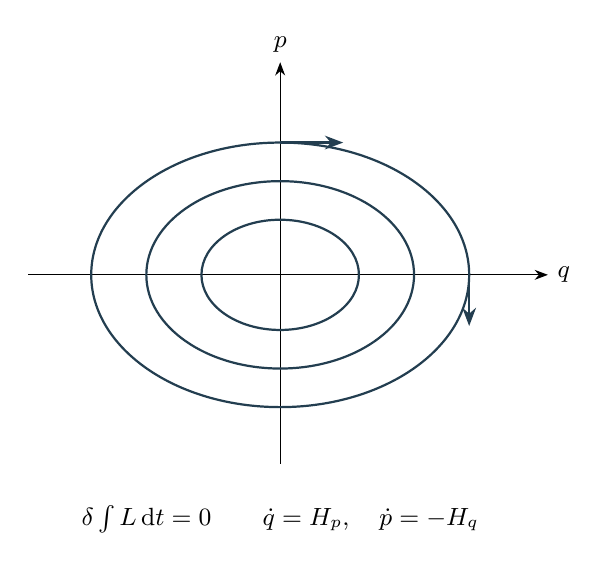
\begin{tikzpicture}[scale=1.0]
\draw[->](-3.2,0)--(3.4,0)node[right]{$q$};\draw[->](0,-2.4)--(0,2.7)node[above]{$p$};
\foreach \a in {1,1.7,2.4}{\pgfmathsetmacro{\b}{.7*\a}\draw[ink,thick](0,0)ellipse(\a cm and \b cm);}
\draw[force](2.4,0)--(2.4,-.65);\draw[force](0,1.68)--(.8,1.68);
\node[fill=white,inner sep=5pt]at(0,-3.1){$\delta\int L\,\dd t=0\qquad\dot q=H_p,\quad\dot p=-H_q$};
\end{tikzpicture}\vfill
{\normalsize 定义与证明\quad 完整例题\quad 图解推导\quad 训练题与解答\par}\vspace{10mm}\end{titlepage}
\pagenumbering{roman}
\section*{符号与基本约定}
分析力学把受约束的运动写成适合求解的方程。第一条线索从虚位移出发，通过理想约束消去未知反力，得到虚功原理和拉格朗日方程。第二条线索以作用量为对象，通过变分把运动方程、对称性与守恒律联系起来。第三条线索把广义速度换成广义动量，建立哈密顿正则方程，再用泊松括号、正则变换和哈密顿--雅可比方程研究运动。

本章先研究有限自由度系统，再把坐标推广为场函数。小振动、相空间和连续系统各自沿着上述线索展开。例题中的运动关系须在题目规定的约束有效范围内使用；单面接触、弹性绳、纯滚动均须额外检查反力、拉力或静摩擦条件。

除明确说明的推广外，质量为常数，约束完整且理想；参考系为惯性系。时间相关的坐标变换会改变广义能量与机械能之间的关系。一阶“驻值”条件都是一阶必要条件，稳定性或极小性需要二阶分析。量子、流体和相对论部分用于说明分析力学结构的延伸，并分别交代附加的物理假设。
\begin{center}\small
\begin{tabularx}{\linewidth}{@{}lX@{}}\toprule
符号&含义\\\midrule
$N,s,k$&质点数、自由度数、独立完整约束数\\
$q_i,\dot q_i,p_i$&广义坐标、广义速度、共轭动量\\
$Q_i,R_i$&主动力与约束力对应的广义力\\
$T,V,L=T-V$&动能、势能、拉格朗日函数\\
$\mathcal E=\sum_i p_i\dot q_i-L$&广义能量；勒让德变换后记为 $H$\\
$S,W$&哈密顿主函数与特性函数\\
$M,K$&小振动的质量矩阵与刚度矩阵\\
$\PB{f}{g}$&泊松括号，规定 $\PB{q_i}{p_j}=\delta_{ij}$\\
$\rho,\mathcal L$&相空间概率密度、拉格朗日密度（具体章节另注明质量密度）\\\bottomrule
\end{tabularx}\end{center}

\clearpage
\begingroup\fontsize{10}{12}\linespread{1}\selectfont\makeatletter
\renewcommand{\@pnumwidth}{2.2em}\renewcommand{\@tocrmarg}{3.2em}
\renewcommand*\l@section[2]{\addvspace{4pt}\@dottedtocline{1}{0em}{3.5em}{\bfseries #1}{\bfseries #2}}
\renewcommand*\l@subsection{\@dottedtocline{2}{1.5em}{4.5em}}
\makeatother\tableofcontents\endgroup\clearpage\pagenumbering{arabic}


\section{约束、自由度与广义坐标}\label{sec:constraints}
\subsection{约束方程及其分类}
约束是限制系统可能位置或速度的条件。约束方程描述这种限制，约束力则是保证限制得以实现的力；二者不能互相代替。例如一根长度为 $l$ 的刚性杆连接两点，其位置条件为 $|\vect r_2-\vect r_1|^2-l^2=0$，杆力仍由动力学求出。

不显含时间的约束称为定常约束，例如 $x^2+y^2=l^2$。显含时间的约束称为非定常约束，例如摆的悬点按已知规律 $a(t)$ 移动时，$(x-a(t))^2+y^2=l^2$。几何约束直接限制位置；运动约束包含速度。限制的方向也不同：刚性杆保持等式，是双面约束；绳只能阻止两端距离超过绳长，是单面约束。在绳绷紧的阶段可用等式，松弛后必须改用另一套运动方程。
\TeachingFigure{c5-diagram-01}{双面约束与单面约束的力学差别}

\OriginalFigure{c5-1-p002-fixed-pivot}{固定悬点的等长单摆}

\OriginalFigure{c5-1-p002-moving-pivot}{悬点以水平速度移动的等长单摆}

\OriginalFigure{c5-1-p003-rigid-pendulum}{刚杆对摆球施加双面长度约束}

\OriginalFigure{c5-1-p003-string-pendulum}{轻绳的张紧与松弛对应单面约束}
\subsection{完整约束与可积的运动约束}
能写成 $f_\alpha(\vect r_1,\ldots,\vect r_N,t)=0$ 的约束为完整约束。运动约束若可积分成这种位置关系，也属于完整约束。例如圆盘沿固定直线纯滚动，$\dot x-R\dot\varphi=0$，积分得 $x-R\varphi=C$。它使 $x$ 与 $\varphi$ 不能独立选取。

一般的线性速度约束写成
\[
\sum_j a_{\alpha j}(q,t)\dot q_j+a_{\alpha0}(q,t)=0.
\]
若对应的微分形式恰为某函数的全微分，或乘以非零积分因子后可化为全微分，则能积分。对已给定的全微分候选 $\sum_j a_j\dd q_j$，局部必要条件是 $\partial_k a_j=\partial_j a_k$；在单连通区域内该条件也是恰当微分的充分条件。一般 Pfaff 约束的可积性比逐项检查偏导更宽，不能把“没有立即找到全微分”当成非完整性的证明。


\example{沿曲线滚动的竖直圆盘}
\label{ex:c5-1}
\QuestionStatement{半径 $R$ 的竖直圆盘在水平面上纯滚动，可自由改变航向。盘心投影为 $(x,y)$，航向角为 $\theta$，自转角为 $\varphi$。写出无侧滑与无纵滑约束，证明它们不是与运动历史无关的位置约束；再讨论沿预定导轨滚动的情形。航向角从固定 $+x$ 方向逆时针计，$\varphi$ 的正向规定为沿航向向前滚动；只讨论盘保持竖直且接触未滑动的阶段。}{ex01}{例1的条件与模型}
\solution \Step{坐标、方向与模型关系}
结合题图\ref{fig:question-ex01}，解答图\ref{fig:solution-ex01}展示同一总滚动弧长、同一末航向对应的不同终点；位置必须沿航向变化的全过程积分。
 在本题模型中，盘面切向由航向角 $\theta$ 决定；沿路径累积的两分量会随航向变化，不能只按终态自转角计算位移。

\Step{方程与推导}
\[\dd x=R\cos\theta\,\dd\varphi,\qquad\dd y=R\sin\theta\,\dd\varphi.\]
\SolutionFigure{ex01}{例1的分析与计算过程}

若位置可仅由 $(\theta,\varphi)$ 决定，第一式要求 $x_\varphi=R\cos\theta$ 且 $x_\theta=0$。于是 $x_{\varphi\theta}=-R\sin\theta$，而 $x_{\theta\varphi}=0$，一般不相等。第二式同样矛盾。滚动后的位移依赖于方向改变的历史，不能把两式积分成与路径无关的两个位置约束。这是非完整约束的典型实例。
更一般地，只看无侧滑的一形式 $\alpha=\sin\theta\dd x-\cos\theta\dd y$。若存在非零积分因子 $g(x,y,\theta)$ 使 $g\alpha=\dd F$，则 $F_\theta=0$，混合偏导要求
\[
\partial_\theta(g\sin\theta)=0,\qquad
\partial_\theta(g\cos\theta)=0.
\]
展开后为 $g_\theta\sin\theta+g\cos\theta=0$ 和 $g_\theta\cos\theta-g\sin\theta=0$。第一式乘 $\cos\theta$、第二式乘 $\sin\theta$ 后相减，得 $g=0$，与非零积分因子矛盾。因而连这一个无侧滑约束也不能局部化为一个位置等式。这比只假定 $x(\theta,\varphi)$ 的检验更直接地排除了积分因子。若圆盘的轨迹已被固定导轨指定、航向由轨迹切线决定，则可用沿轨道的弧长 $s$，滚动关系 $s-R\varphi=C$ 是完整约束；不能仅凭轨迹弯曲就判为非完整。

\OriginalFigure{c5-1-p004-straight-rolling-disk}{圆盘沿直线纯滚动：向右平移与顺时针自转}

\OriginalFigure{c5-1-p028-steering-disk}{自由转向圆盘的航向$\theta$与平面轨迹；图中半径a对应正文R}
\subsection{自由度计数与独立性}
$N$ 个自由质点的位置需要 $3N$ 个笛卡儿坐标。若有 $k$ 个独立完整约束，且约束梯度的秩为 $k$，则局部自由度为
\begin{equation}s=3N-k.\label{eq:dof}\end{equation}
“独立”不可省略：同一约束重复写两遍，不会再减少自由度；机构的特殊位置可能使约束秩改变。平面问题先限定每个质点只有两个位置变量，再扣除独立约束。非完整约束限制可取速度，通常不使构形空间的维数减少相同数量。

广义坐标是描述构形所需的 $s$ 个局部独立变量 $q_1,\ldots,q_s$。它们可以是长度、角度或混合变量，量纲不必相同。所有位置应能写成
\[
\vect r_a=\vect r_a(q_1,\ldots,q_s,t),\qquad
\vect v_a=\sum_i\frac{\partial\vect r_a}{\partial q_i}\dot q_i+\frac{\partial\vect r_a}{\partial t}.
\]
坐标是构形的标记；完整运动状态还须给出广义速度或共轭动量。
\subsection{常见系统的坐标选择}

\example{单摆、球面质点、滚动圆盘与定点刚体}
\label{ex:c5-2}
\LongQuestionStatement{分别确定下列系统的局部自由度并选取广义坐标：竖直平面内长 $l$ 的刚杆单摆；半径 $R$ 的球面质点；沿固定直线纯滚动的圆盘；固定一点、可在三维空间转动的刚体。说明约束独立性和姿态坐标奇点的含义。各长度、半径均为正；直线滚动时自转角的正向与向前位移相容。这里的姿态参数描述材料刚体，不能把轴对称外形当作材料点不可区分。}{ex02}{例2的条件与模型}
\solution \Step{坐标、方向与模型关系}
结合题图\ref{fig:question-ex02}，解答图\ref{fig:solution-ex02}展示杆长约束消去的径向位移与球面上的两个切向位移；直线滚动约束连接平移和自转，定点刚体仍保留三个姿态自由度。
 在本题模型中，摆长、球半径与直线滚动约束各消去一个独立位置变量；定点刚体还保留三个姿态参数。


\SolutionFigure{ex02}{例2的分析与计算过程}
\Step{方程与推导}
单摆在竖直平面内运动，两个位置变量加一个杆长约束，$s=1$，可取 $\theta$。球面质点三个位置变量加一个半径约束，$s=2$，可取 $(\theta,\phi)$。沿直线滚动圆盘用 $(x,\varphi)$ 描述，滚动约束后 $s=1$，可取其中任一个。定点刚体的位置由姿态决定，$s=3$，可取欧拉角；其坐标表示在特殊姿态会出现奇点，奇点不意味着物理自由度减少。
\TeachingFigure{c5-diagram-03}{几种完整约束系统的广义坐标}

\Step{约束数的逐项计算} 单摆的位置为 $(x,y)$，约束 $x^2+y^2=l^2$ 在 $l>0$ 时梯度非零，故 $2-1=1$。球面在 $R>0$ 时同理为 $3-1=2$。直线滚动先以 $(x,\varphi)$ 描述，再施加 $x-R\varphi=C$，得到 $2-1=1$。三维刚体的自由构形原有三平移、三转动；固定一个材料点消去三平移，余下三转动。欧拉角在极点的退化是坐标映射秩降低，可以更换姿态坐标，并非物体失去某个转动。


\OriginalFigure{c5-1-p007-euler-angles}{定点刚体的三个欧拉角；角弧表示夹角，正方向按正文约定}
\example{螺旋线、平面定点运动与三维定点运动}
\label{ex:c5-3}
\LongQuestionStatement{质量 $m$ 的质点被限制在螺旋线 $x=a\cos u,y=a\sin u,z=bu$ 上，$a>0$，求自由度、弧长元及动能。另比较平面内定点刚体和三维定点刚体的自由度，说明轴对称外形是否可以省去材料自转角。螺旋参数 $u$ 为无量纲角，$b$ 为给定常量，量纲为长度；平面定点刚体仅允许在该固定平面内转动。}{ex03}{例3的条件与模型}
\solution \Step{坐标、方向与模型关系}
结合题图\ref{fig:question-ex03}，解答图\ref{fig:solution-ex03}展示螺旋线展开后的弧长三角形；同一参数增量同时产生水平圆周增量和竖直增量，二者平方相加得到动能系数。
 在本题模型中，螺旋线的轴向升高和水平绕转都由同一参数 $u$ 决定，弧长中两部分的平方相加。


\SolutionFigure{ex03}{例3的分析与计算过程}
\Step{方程与推导}
螺旋线由 $x=a\cos u,y=a\sin u,z=bu$ 给定，$a>0$。质点只能沿这条曲线运动，所以只有一个自由度。弧长微分是 $\dd s=\sqrt{a^2+b^2}\dd u$，既可取无量纲参数 $u$，也可取有长度量纲的 $s$。沿线动能分别为 $m(a^2+b^2)\dot u^2/2$ 与 $m\dot s^2/2$，两种坐标给同一运动。

刚体限制在平面内且固定一点时，任意姿态只需一个转角 $\gamma$；允许它在三维空间绕固定点转动时，需三个独立姿态参数，例如欧拉角 $(\phi,\theta,\psi)$。固定点减少平动自由度，但不把三维转动压成一个自由度。轴对称物体的外形虽可能不显示自转角，带标记的材料点仍由 $\psi$ 决定。

\Step{由参数得到弧长} 若定点刚体质心距支点为 $d$，在给定平面可写 $x_C=d\sin\gamma,y_C=-d\cos\gamma$。在 $d\cos\gamma\ne0$ 或 $d\sin\gamma\ne0$ 的局部范围分别可用 $x_C$ 或 $y_C$ 作坐标；转折处须换坐标，$d=0$ 时质心位置完全不能描述姿态。对三坐标求导，$\vect r_u=(-a\sin u,a\cos u,b)$，所以 $\vect r_u^2=a^2+b^2$。有向弧长坐标可取 $s=\sqrt{a^2+b^2}(u-u_0)$；实际弧长增量取 $\lvert\dd s\rvert$。这使 $m\dot s^2/2=m(a^2+b^2)\dot u^2/2$，并不产生额外自由度。


\OriginalFigure{c5-1-p007-helix}{约束在给定螺旋线上的质点}

\OriginalFigure{c5-1-p007-planar-fixed-body}{刚体在竖直平面内绕固定点O摆动；图中$\theta$对应正文$\gamma$}
\example{弹性阿特伍德系统与受驱动圆环}
\label{ex:c5-4}
\LongQuestionStatement{理想定滑轮两侧以不可伸长主绳连接重物，一侧重物下方再用可伸缩轻弹簧悬挂另一重物。选取主绳一侧向下位移 $y$ 和弹簧长度 $s$，判断自由度。另有圆环绕环上一点的固定竖直轴在水平面内按已知角度 $\alpha(t)$ 转动，滑珠可沿环移动：判断规定转动和自由转动时各有几个自由度。具体规定 $y$ 为连接弹簧一侧的上重物向下坐标，$s>0$；三个重物的位置均沿各自竖直运动线计量。圆环的“自由转动”仍绕同一固定轴，而非解除全部支承。}{ex04}{例4的条件与模型}
\solution \Step{坐标、方向与模型关系}
结合题图\ref{fig:question-ex04}，解答图\ref{fig:solution-ex04}展示主绳两侧互相制约的虚位移与弹簧下端的附加虚位移；弹簧长度并未被主绳固定，因此需要两个坐标。
 在本题模型中，主绳把两侧位移联系起来，却不固定下面弹簧的长度 $s$；驱动环的整体角 $\alpha(t)$ 已由外界规定。


\SolutionFigure{ex04}{例4的分析与计算过程}
\Step{方程与推导}
弹性阿特伍德系统中，主绳不可伸长，只消去两侧滑轮下端之间的一个长度变量；一侧弹簧可以伸缩，下端质点的位置仍独立。故可取一个主绳位移和一个弹簧长度，共两个自由度。圆环按规定角速度绕其圆周上的固定轴转动时，转角是已知的时间函数，不能再算作独立坐标；环上滑珠只需一个沿圆周角。若圆环的转速也由动力学决定而未规定，则还需加入它自己的转角。自由度判断依赖于装置的具体限制。

\Step{独立坐标及位置映射} 忽略绕轮部分的常长度，主绳给 $y_L+y_R=C$。取 $y=y_R$、弹簧长度 $s$，则三个重物的位置分别为 $C-y,y,y+s$；任意微小 $\delta y,\delta s$ 均可独立指定，故为两个自由度。驱动圆环的珠位置可写为 $\vect r=\mathsf R[\alpha(t)]\vect r_{\rm ring}(\theta)$，只有 $\theta$ 待求；若不规定 $\alpha$，则 $(\alpha,\theta)$ 均须参与动力学，得到两个自由度。这里自由转动仍保留固定轴，未解除圆环支承。

\OriginalFigure{c5-1-p007-elastic-atwood}{绳轮连接的三球系统；滑轮旁的a为滑轮半径，正文a为弹性绳自然长}

\OriginalFigure{c5-1-p007-driven-hoop}{圆环绕环上固定点O匀速转动，滑珠位置用相对角$\theta$描述}
\section{虚位移、广义力与虚功原理}\label{sec:virtual}
\subsection{等时虚位移与实位移}
虚位移是在同一时刻、满足约束的邻近构形之间的无限小差。它不要求系统真的按这条方向运动，不包含时间推进。在完整约束下
\begin{equation}
\delta\vect r_a=\sum_i\frac{\partial\vect r_a}{\partial q_i}\delta q_i,
\qquad \sum_a\nabla_a f_\alpha\cdot\delta\vect r_a=0.\label{eq:virtual}
\end{equation}
实位移则满足
\[
\dd\vect r_a=\sum_i\vect r_{a,q_i}\dd q_i+\vect r_{a,t}\dd t,
\qquad\sum_a\nabla_a f_\alpha\cdot\dd\vect r_a+f_{\alpha,t}\dd t=0.
\]
因此非定常约束下，两者连允许方向也可能不同。定常约束下允许方向相同，但真实位移由运动方程决定，虚位移仍可任意取为约束切空间中的方向。
\TeachingFigure{c5-diagram-05}{移动约束面上的虚位移与实位移}

\OriginalFigure{c5-1-p008-linkage-virtual}{曲柄连杆机构的两组许可虚位移}

\OriginalFigure{c5-1-p008-surface-virtual}{约束曲面上不同方向的切向虚位移}
\subsection{虚位移的直接计算}

\example{单摆与球面上的虚位移}
\label{ex:c5-5}
\LongQuestionStatement{分别求允许虚位移：（1）长 $l$ 的平面单摆，摆角 $\theta$ 从竖直向下量起；（2）半径 $R$ 的球面质点，采用极角 $\theta$ 和方位角 $\phi$。用图中的切向基矢表示结果，并说明与径向反力的关系。}{ex05}{例5的条件与模型}
\solution \Step{坐标、方向与模型关系}
结合题图\ref{fig:question-ex05}，解答图\ref{fig:solution-ex05}展示允许虚位移与约束径向正交；只有主动力沿切向的投影进入虚功和广义力，径向反力不能重复加入。
 在本题模型中，圆周切向对应单摆唯一变分方向；球面的两个切向箭头分别对应独立的极角、方位角变分。

\Step{方程与推导}
单摆以竖直向下为 $\theta=0$，$x=l\sin\theta,y=-l\cos\theta$，故
\[
\delta x=l\cos\theta\,\delta\theta,\quad\delta y=l\sin\theta\,\delta\theta,
\quad\delta\vect r=l\vect e_\theta\delta\theta.
\]
\SolutionFigure{ex05}{例5的分析与计算过程}

球面质点用通常球坐标，$\vect r=R\vect e_r$，则
\[
\delta\vect r=R\vect e_\theta\delta\theta+R\sin\theta\vect e_\phi\delta\phi.
\]
两者的虚位移均垂直于径向反力。球面的两个切向方向可以独立变化，不应把虚位移限定为实际轨迹的切线。

\Step{坐标偏导与法向正交} 单摆 $\vect r_\theta=l(\cos\theta,\sin\theta)$，与 $\vect r=l(\sin\theta,-\cos\theta)$ 点积为零。球面常规参数为 $R(\sin\theta\cos\phi,\sin\theta\sin\phi,\cos\theta)$；其两个偏导分别为 $R\vect e_\theta$、$R\sin\theta\vect e_\phi$，两者与 $\vect e_r$ 的点积均为零，因而法向反力对任何允许虚位移都不作功。展开成分量为 $\delta x=R\cos\theta\cos\phi\delta\theta-R\sin\theta\sin\phi\delta\phi$，$\delta y=R\cos\theta\sin\phi\delta\theta+R\sin\theta\cos\phi\delta\phi$，$\delta z=-R\sin\theta\delta\theta$。极点处方位角参数退化，球面切空间仍为二维。

\OriginalFigure{c5-1-p014-pendulum-displacement}{单摆的位矢与摆角$\theta$}
\subsection{虚功与广义力}
主动力的虚功是
\[
\delta W=\sum_a\vect F_a\cdot\delta\vect r_a
=\sum_i Q_i\delta q_i,
\qquad Q_i=\sum_a\vect F_a\cdot\frac{\partial\vect r_a}{\partial q_i}.
\]
$Q_i\delta q_i$ 的量纲总是能量。若 $q_i$ 是长度，$Q_i$ 量纲为力；若 $q_i$ 为角度，$Q_i$ 量纲为力矩。但它不必等于某一质点的受力或某一轴上的总力矩，具体含义由位置对坐标的导数决定。

保守力 $\vect F_a=-\nabla_aV$ 在等时变分下满足 $Q_i=-\partial_i V$。若存在未包含在势能中的力，将其广义力另外记为 $Q_i^{\rm nc}$。

\example{水平力对单摆的广义力}
\label{ex:c5-6}
\QuestionStatement{长 $l$、球质量 $m$ 的单摆受向右恒力 $F$ 和重力。摆角 $\theta$ 从竖直向下向右量起，求广义力与势能。令 $F=0$，比较轻绳和可推可拉刚杆在正立、倒立位置的平衡与稳定性。}{ex06}{例6的条件与模型}
\solution \Step{坐标、方向与模型关系}
结合题图\ref{fig:question-ex06}，解答图\ref{fig:solution-ex06}展示允许虚位移与约束径向正交；只有主动力沿切向的投影进入虚功和广义力，径向反力不能重复加入。
 在本题模型中，水平力沿 $+x$、重力沿 $-y$；两力分别与摆球切向位移投影相乘，产生正负不同的广义力。

\Step{方程与推导}
摆球受水平向右的力 $F$ 和重力 $mg$。直接用位移分量求得
\[
\delta W=(Fl\cos\theta-mgl\sin\theta)\delta\theta,
\qquad Q_\theta=Fl\cos\theta-mgl\sin\theta.
\]
\SolutionFigure{ex06}{例6的分析与计算过程}

等价地取 $V=-Fl\sin\theta-mgl\cos\theta$。这里 $Q_\theta$ 是相对悬点、沿正转角方向的合力矩。特别令 $F=0$，则 $\delta W=-mgl\sin\theta\,\delta\theta$，静力条件是 $\sin\theta=0$。轻绳的有效张紧平衡为 $\theta=0$；可推可拉的刚杆还允许 $\theta=\pi$，但倒立支不稳定。轻绳在倒立位置需要负张力，因而该形式驻值不能作为其真实平衡。

\Step{平衡与稳定分支} 对于 $F\ne0$，写 $V=-ml\sqrt{g^2+(F/m)^2}\cos(\theta-\theta_e)$，其中 $\tan\theta_e=F/(mg)$、$\cos\theta_e>0$。下垂分支 $V''(\theta_e)=l\sqrt{F^2+m^2g^2}>0$，稳定。$F=0$ 时 $V''(0)=mgl>0$、$V''(\pi)=-mgl<0$；静止径向平衡要求 $T=mg\cos\theta$，故倒立绳支的 $T=-mg$ 不可实现。
\subsection{理想约束及其适用范围}
若所有约束力对任意允许虚位移的总虚功为零，约束称为理想约束。光滑支承面的反力垂直切向位移；固定光滑铰链的受力点不移动；内部光滑铰链的共同铰点虽可移动，但两物体所受反力相反，合虚功抵消；刚性轻杆两端的力成对，其虚功和因杆长不变而为零。不可伸长的轻绳在绷紧并配合理想滑轮的条件下，也具有这样的抵消。

固定粗糙面上的纯滚动可以是理想约束：接触点瞬时速度为零，允许的接触虚位移也为零，静摩擦不作虚功。它仍会改变质心动量，并可在质心平动能与转动能之间转移能量。滑动摩擦一般不是理想约束力，须作为主动力计入。
\TeachingFigure{c5-diagram-06}{理想约束的零总虚功来自几何垂直、反力抵消或接触点不动}


\OriginalFigure{c5-1-p010-smooth-support}{光滑支承面的法向力与切向虚位移}

\OriginalFigure{c5-1-p010-ideal-hinge}{内铰链两侧反力相反，铰点虚位移相同}

\OriginalFigure{c5-1-p010-rolling-contact}{纯滚动接触点C处的法向力N与静摩擦F}
\subsection{虚功原理的证明与势能判据}
在定常、双面、理想约束下，静力平衡当且仅当
\begin{equation}\sum_a\vect F_a\cdot\delta\vect r_a=0
\quad\text{对任意允许虚位移成立},\qquad Q_i=0.\label{eq:vw}\end{equation}
必要性：把每个质点的平衡方程 $\vect F_a+\vect R_a=0$ 与虚位移点乘并求和，约束虚功消失。充分性：独立 $\delta q_i$ 的系数全部为零，主动力在构形空间的切向分量为零，剩余法向分量可由理想约束反力平衡。在已知单面约束上，反力还须满足可实现的符号条件。

保守系统平衡位置满足 $\delta V=0$，即势能驻值。局部严格极小值对应稳定平衡的常用充分条件；极大值通常不稳定。不能把所有平衡都写成“势能取极小值”。


\TeachingFigure{c5-diagram-07}{平衡位置与稳定性需分别判断}
\subsection{两根均匀铰接杆的静力平衡}


\example{端点水平力作用下的两杆}
\label{ex:c5-7}
\QuestionStatement{均匀杆 $OA,AB$ 长 $l_1,l_2$，重 $P_1,P_2$，在竖直平面内光滑铰接；$O$ 固定，$B$ 受向右恒力 $F$。两杆角 $\theta_1,\theta_2$ 均从竖直向下量起。用虚功法求稳定下垂平衡构形，并写出势能验证。}{ex07}{例7的条件与模型}
\solution \Step{坐标、方向与模型关系}
结合题图\ref{fig:question-ex07}，解答图\ref{fig:solution-ex07}展示两杆质心重力和端点外力；上杆转动会同时移动下杆及其质心，虚功系数必须包括这一部分。
 在本题模型中，两杆角互相独立；第二杆重心随铰点 $A$ 移动，因此第一角的重力系数还包含整根第二杆的重量。

\Step{方程与推导}
两个角独立。取 $X$ 向右、$Y$ 向上，先写出两个质心和受力端点的坐标：
\begin{align*}
X_{C_1}&=\frac{l_1}{2}\sin\theta_1,&Y_{C_1}&=-\frac{l_1}{2}\cos\theta_1,\\
X_{C_2}&=l_1\sin\theta_1+\frac{l_2}{2}\sin\theta_2,
&Y_{C_2}&=-l_1\cos\theta_1-\frac{l_2}{2}\cos\theta_2,\\
X_B&=l_1\sin\theta_1+l_2\sin\theta_2.
\end{align*}
\SolutionFigure{ex07}{例7的分析与计算过程}

第二杆的质心随第一杆的铰点移动，故第一角对应的重力项包含 $P_2$。铰链光滑，反力的总虚功抵消，主动力虚功为
\begin{align*}
\delta W&=-P_1\delta Y_{C_1}-P_2\delta Y_{C_2}+F\delta X_B\\
&=l_1\left[F\cos\theta_1-\left(\frac{P_1}{2}+P_2\right)\sin\theta_1\right]\delta\theta_1\\
&\quad+l_2\left(F\cos\theta_2-\frac{P_2}{2}\sin\theta_2\right)\delta\theta_2.
\end{align*}
两个允许角变分相互独立，因此两个系数分别为零。亦可把水平恒力纳入势能；两个质心和端点的坐标给出
\[
V=-\left(\frac{P_1}{2}+P_2\right)l_1\cos\theta_1
-\frac{P_2l_2}{2}\cos\theta_2
-F(l_1\sin\theta_1+l_2\sin\theta_2).
\]
所以
\[
\left(\frac{P_1}{2}+P_2\right)\sin\theta_1=F\cos\theta_1,
\qquad \frac{P_2}{2}\sin\theta_2=F\cos\theta_2.
\]
稳定的下垂分支满足 $\tan\theta_1=2F/(P_1+2P_2)$，$\tan\theta_2=2F/P_2$。若把角改从水平线向下量起，$\alpha=\pi/2-\theta_1,\beta=\pi/2-\theta_2$，则 $\tan\alpha=(P_1+2P_2)/(2F),\tan\beta=P_2/(2F)$。没有必要先求三个铰链反力；计算反力时再回到各杆的平衡方程。

\OriginalFigure{c5-1-p018-two-rods-static}{两铰接杆的静力构形：$\alpha$=$\pi$/2-$\theta_1$，$\beta$=$\pi$/2-$\theta_2$；图中x向下、y向右}
\subsection{三个机构点的虚位移与坐标奇点}

\example{等长连杆机构的三个位置映射}
\label{ex:c5-8}
\QuestionStatement{固定点 $O$ 与杆 $OA$ 长 $l$，点 $C$ 在杆上，$OC=CB=a$；$B$ 沿过 $O$ 的水平直线滑动。取 $OA$ 与水平线夹角 $\phi$，采用 $B$ 位于右侧的构形。写 $A,C,B$ 的位置和虚位移，并解释 $\phi=0$ 时用 $x_B$ 作坐标的局限。设 $0<a<l$，$|\phi|<\pi/2$；选择非重合的右侧滑块支，$x_B>0$，而非退化的 $B=O$ 支。}{ex08}{例8的条件与模型}
\solution \Step{坐标、方向与模型关系}
结合题图\ref{fig:question-ex08}，解答图\ref{fig:solution-ex08}展示同一角变分引起的三个点位移方向；$A,C$ 的虚位移分别垂直各自转臂，$B$ 不能再有独立竖向位移。
 在本题模型中，点 $A,C$ 的切向虚位移共用 $\delta\phi$；滑块 $B$ 只作水平位移，不能再赋予独立竖向变分。

\Step{方程与推导}
$O$ 固定，$OA=l$，$C$ 在 $OA$ 上，$OC=CB=a$，$B$ 沿过 $O$ 的水平线滑动；取 $OA$ 与水平夹角 $\phi$，采用右侧构形。位置为
\[
\vect r_A=l(\cos\phi,\sin\phi),\quad\vect r_C=a(\cos\phi,\sin\phi),\quad\vect r_B=(2a\cos\phi,0).
\]
\SolutionFigure{ex08}{例8的分析与计算过程}

因此 $\delta\vect r_A=l(-\sin\phi,\cos\phi)\delta\phi$，$\delta\vect r_C=a(-\sin\phi,\cos\phi)\delta\phi$，$\delta\vect r_B=(-2a\sin\phi,0)\delta\phi$。$B$ 只有水平虚位移，$A,C$ 的位移与各自转臂垂直。$\phi=0$ 时 $\delta x_B=0$，用 $x_B$ 替代 $\phi$ 的坐标映射此处失去局部可逆性。

\Step{约束微分与奇异位置} 连杆约束为 $(x_B-a\cos\phi)^2+a^2\sin^2\phi=a^2$。右支取 $x_B=2a\cos\phi$，与图中机构一致。局部反解需要 $\dd x_B/\dd\phi=-2a\sin\phi\ne0$；在 $\phi=0$，小角度改变只产生二阶滑块位移 $x_B=2a-a\phi^2+O(\phi^4)$，因此一阶速度不能唯一反推出角速度。

\OriginalFigure{c5-1-p029-three-point-linkage}{机构A、B、C三点的虚位移，OC=CB=a，OA=l}
\subsection{墙与棱边支承杆的平衡及稳定性}


\example{均匀杆跨过固定光滑棱边}
\label{ex:c5-9}
\QuestionStatement{长 $2l$、质量 $m$ 的均匀杆，下端 $A$ 靠在固定光滑竖直墙上，杆身跨过距墙水平距离 $d$ 的固定光滑棱边 $O$，$0<d<l$。杆向右上方伸出，与水平夹角 $\theta$。求平衡角、稳定性及两处反力，并说明接触点确在杆上。}{ex09}{例9的条件与模型}
\solution \Step{坐标、方向与模型关系}
结合题图\ref{fig:question-ex09}，解答图\ref{fig:solution-ex09}展示光滑墙面、光滑棱边的两种不同法向及质心重力；取矩和虚功时应使用实际支承几何，不能把两反力都画成竖直。
 在本题模型中，固定棱边 $O$ 限制杆与墙的交点高度；杆重心 $C$ 的高度随两种几何效应同时变化。

\Step{方程与推导}
固定 $O$ 高度为零，有 $AO=d/\cos\theta$，$y_A=-d\tan\theta$，$y_C=l\sin\theta-d\tan\theta$。重力虚功给出
\[
\delta W=-mg(l\cos\theta-d\sec^2\theta)\delta\theta=0,
\quad\cos^3\theta=\frac dl.
\]
\SolutionFigure{ex09}{例9的分析与计算过程}

但 $V''=-3mgl\sin\theta<0$，所以这是真实可行的不稳定静平衡，不能把静力条件一律称为势能极小。棱边法向力为 $N_O=mg/\cos\theta$，墙反力 $N_A=N_O\sin\theta$，均为正；这检验了两处单面接触的可实现性。$AO=l\cos^2\theta<l$，接触点位于杆中点之前，与构形一致。

\OriginalFigure{c5-1-p016-wall-edge-rod}{均匀杆AB跨过光滑棱边O，C为中点，杆长2l}
\subsection{直角折杆的平衡角}


\example{两段同线密度杆构成的刚性折杆}
\label{ex:c5-10}
\QuestionStatement{两根同线密度 $\sigma$ 的均匀细杆 $AB=a,BC=b$ 刚接成直角折杆，以 $A$ 光滑悬挂。取 $AB$ 向左偏离竖直向下角为 $\theta$，$BC$ 向右下方。求稳定平衡角，写出两段质心高度和总势能。给定 $a,b,\sigma>0$，忽略铰轴摩擦，重力加速度记为 $g$；两段杆的质量必须分别按实际杆长计算。}{ex10}{例10的条件与模型}
\solution \Step{坐标、方向与模型关系}
结合题图\ref{fig:question-ex10}，解答图\ref{fig:solution-ex10}展示直角折杆两段的质心和重力；两段质量分别为线密度乘杆长，不能对两个质心高度作简单平均。
 在本题模型中，两段质心位置分别按各自杆长和质量加权；铰点 $A$ 的反力不作虚功。

\Step{方程与推导}
两杆质心向下高度为 $y_D=(a/2)\cos\theta$，$y_E=a\cos\theta+(b/2)\sin\theta$。虚功为 $\sigma g[a\delta y_D+b\delta y_E]=0$，所以
\[
-\left(\frac{a^2}2+ab\right)\sin\theta+\frac{b^2}2\cos\theta=0,
\quad\tan\theta=\frac{b^2}{a^2+2ab}.
\]
\SolutionFigure{ex10}{例10的分析与计算过程}

重心法给出同式：整个重心的横坐标为上述左边除以 $a+b$，平衡时重心位于 $A$ 的正下方。在下垂分支势能取极小，因而稳定。

\Step{质心高度与总势能} 两段质心高度分别为 $y_{C_1}=-a\cos\theta/2$、$y_{C_2}=-a\cos\theta-b\sin\theta/2$，所以 $V=-\sigma g[(a^2/2+ab)\cos\theta+(b^2/2)\sin\theta]$。令 $V_\theta=0$ 得 $(a^2+2ab)\sin\theta=b^2\cos\theta$。在下垂分支 $V_{\theta\theta}=\sigma g\sqrt{(a^2/2+ab)^2+b^4/4}>0$，因此该支稳定。

\OriginalFigure{c5-1-p031-right-angle-rod}{直角折杆与两段质心D、E；图中$\theta_0$为平衡角}
\subsection{曲柄连杆的力关系}


\example{一个自由度的曲柄连杆机构}
\label{ex:c5-11}
\QuestionStatement{水平曲柄连杆机构中 $OA=r,AB=l$，$B$ 沿过 $O$ 的水平线滑动。曲柄向右上方与水平成 $\phi$，连杆向右下方成 $\psi$，满足 $r\sin\phi=l\sin\psi$。在 $A$ 处施沿 $\phi$ 增大方向的切向力 $F_A$，$B$ 处施向右力 $F_B$。忽略各杆重量，求静力平衡的力关系。设 $r,l>0$，在满足几何约束且 $\cos\psi\ne0$ 的同一连续装配支上计算。力的代数符号按上述箭头方向规定，不预先限定两外力必须同号。}{ex11}{例11的条件与模型}
\solution \Step{坐标、方向与模型关系}
结合题图\ref{fig:question-ex11}，解答图\ref{fig:solution-ex11}展示曲柄切向外力、滑块外力及相容虚位移；建立力关系时，应将滑块位移对曲柄角的导数完整代入。
 在本题模型中，曲柄的切向力与弧向虚位移同向；滑块位移受连杆长度约束，符号由右正方向确定。

\Step{方程与推导}
几何关系是 $r\sin\varphi=l\sin\psi$ 和 $x_B=r\cos\varphi+l\cos\psi$。等时变分给出
\[
l\cos\psi\,\delta\psi=r\cos\varphi\,\delta\varphi,
\quad \delta x_B=-r(\sin\varphi+\cos\varphi\tan\psi)\delta\varphi.
\]
\SolutionFigure{ex11}{例11的分析与计算过程}

$A$ 的切向位移为 $r\delta\varphi$，故
\[
\delta W=F_A r\delta\varphi+F_B\delta x_B=0,
\qquad F_A=F_B\frac{\sin(\varphi+\psi)}{\cos\psi}.
\]
所以 $F_B/F_A=\cos\psi/\sin(\varphi+\psi)$；转角和箭头方向均应按题设使用。死点附近须单独看几何极限，不能在 $\cos\psi=0$ 时直接除以它。

\OriginalFigure{c5-1-p032-crank-forces}{曲柄连杆的几何尺寸与主动力方向}

\OriginalFigure{c5-1-p033-crank-virtual}{曲柄连杆的许可虚转动与两作用点虚位移}
\section{拉格朗日乘数与约束反力}\label{sec:multipliers}
\subsection{受约束的极值问题}
用冗余坐标 $x_1,\ldots,x_n$，在 $k$ 个约束 $f_\alpha(x)=0$ 下求 $V(x)$ 的驻值。若约束梯度独立，存在乘数使
\[
\Phi=V-\sum_\alpha\lambda_\alpha f_\alpha,
\quad \partial_jV-\sum_\alpha\lambda_\alpha\partial_j f_\alpha=0,
\quad f_\alpha=0.
\]
乘数和坐标一同求解。约束函数乘以常数后，乘数反向缩放，因此乘数本身没有固定的力学意义；真正的约束广义力是 $R_j=\sum_\alpha\lambda_\alpha\partial_j f_\alpha$。

\example{抛物面上与平面、圆柱相交的极值}
\label{ex:c5-12}
\LongQuestionStatement{曲面为 $z=x^2+y^2$。分别在（1）平面 $x+y=1$；（2）圆柱 $(x-2)^2+y^2=1$ 的约束下，求高度 $z$ 的极值、位置和是否存在最大值。用拉格朗日乘数法并说明约束交线的几何含义。}{ex12}{例12的条件与模型}
\solution \Step{坐标、方向与模型关系}
结合题图\ref{fig:question-ex12}，解答图\ref{fig:solution-ex12}展示抛物面等高线与两类约束的平面投影；梯度平行对应等高线相切，直线约束无界而圆柱交线有界。
 在本题模型中，投影图中的直线和偏心圆是允许位置；沿约束交线改变位置时，驻值点的高度一阶变化为零。


\SolutionFigure{ex12}{例12的分析与计算过程}
\Step{方程与推导}
求 $z=x^2+y^2$ 在 $x+y=1$ 上的极值。取 $\Phi=x^2+y^2-\lambda(x+y-1)$，两偏导为零得 $2x=2y=\lambda$，所以 $x=y=1/2,z_{\min}=1/2$。也可消去 $y$，得 \mbox{$z=x^2+(1-x)^2=2(x-1/2)^2+1/2$}，直接确认它是全局最小；沿无限交线 $|x|\to\infty$ 时 $z\to\infty$，不存在全局最大值。

改成 $(x-2)^2+y^2=1$，则 $2x=2\lambda(x-2),2y=2\lambda y$。若 $y\ne0$，第二式要求 $\lambda=1$，与第一式矛盾。故 $y=0$，$x=1$ 或 $3$，相应 $z=1$ 或 $9$。圆上函数连续，两个驻值就是全局最小值与最大值。

\OriginalFigure{c5-1-p020-paraboloid-plane}{抛物面与平面相交形成的受约束曲线}

\OriginalFigure{c5-1-p020-paraboloid-cylinder}{抛物面与偏置圆柱面的交线}
\subsection{静力方程与反力恢复}
先用冗余坐标 $x_j$ 保留约束 $f_\alpha(x)=0$。在约束梯度独立、约束理想时，约束反力位于这些梯度的张成空间；用乘数写出反力之后，可以把原受限的变分等价改写为对 $x_j$ 与 $\lambda_\alpha$ 的独立变分：
\begin{align*}
0&=\delta W+\sum_\alpha\lambda_\alpha\delta f_\alpha
+\sum_\alpha f_\alpha\delta\lambda_\alpha\\
&=\sum_j\left(Q_j+\sum_\alpha\lambda_\alpha\frac{\partial f_\alpha}{\partial x_j}\right)\delta x_j
+\sum_\alpha f_\alpha\delta\lambda_\alpha.
\end{align*}
各 $\delta x_j$ 的系数给平衡方程，各 $\delta\lambda_\alpha$ 的系数恢复约束；不能在冗余坐标仍受限时先误称所有 $\delta x_j$ 独立。对一般主动力，乘数形式是
\[
Q_j+\sum_\alpha\lambda_\alpha\partial_j f_\alpha=0,
\qquad f_\alpha=0.
\]
若 $x_j$ 为笛卡儿分量，相应 $R_j$ 是力分量；若为角，$R_j$ 是广义力矩。不能把角坐标的乘数结果直接当成杆轴力。先由定义将轴力的虚功写成坐标的系数，再与 $R_j$ 比较。
\TeachingFigure{c5-diagram-14}{目标函数曲面的高度沿约束交线取驻值，两种几何约束给不同极值}

\subsection{三杆结构的三种求解方式}


\example{顶角为六十度的对称轻杆结构}
\label{ex:c5-13}
\QuestionStatement{轻杆 $AB,BC$ 各长 $2l$，构成顶角 $60^\circ$ 的对称结构；底端 $A,C$ 在同一光滑水平面上，顶点 $B$ 受竖直向下力 $P$。两杆中点 $D,E$ 由长 $l$ 的轻横杆连接。求横杆内力，规定拆去横杆后向外为正，分别用虚功、乘数和整体与单杆平衡说明其拉压性质。所有节点均为理想光滑铰接，三杆均可受拉或受压；内力的正负号与真实拉压性质须在解答中对应说明。}{ex13}{例13的条件与模型}
\solution \Step{坐标、方向与模型关系}
结合题图\ref{fig:question-ex13}，解答图\ref{fig:solution-ex13}展示拆开后的横杆拉力与整体外力；必须区分横杆对斜杆的力和斜杆对横杆的反作用力，才能判断乘数的拉压符号。
 在本题模型中，中点横杆长度是所选位移 $x$；将横杆拆去，向外的正试探力与顶点下降的虚功相联系。

\Step{方程与推导}
取 $x=DE$，则顶点高度 $y_B=\sqrt{4l^2-x^2}$，约束 $f=x-l=0$。主动力广义力为
\[
Q_x=-P\frac{\dd y_B}{\dd x}=P\frac{x}{y_B}.
\]
\SolutionFigure{ex13}{例13的分析与计算过程}

平衡方程 $Q_x+\lambda=0$ 给出 $x=l,y_B=\sqrt3l,\lambda=-P/\sqrt3$。以向外推两端为正，横杆轴力 $N=\lambda$，所以它实际承受大小 $P/\sqrt3$ 的拉力。

第二种方式取 $\theta=\tfrac12\angle ABC$。$y_B=2l\cos\theta$，$DE=2l\sin\theta$。约束 $f=2l\sin\theta-l=0$，平衡给出
\[
2Pl\sin\theta+2\lambda l\cos\theta=0,
\quad\theta=\frac\pi6,\quad\lambda=-\frac P{\sqrt3}.
\]
角坐标的约束广义力为 $R_\theta=2\lambda l\cos\theta$；而横杆对两端的虚功为 $2Nl\cos\theta\delta\theta$，比较系数才得到 $N=\lambda$。

第三种方式暂时拆除横杆，在 $D,E$ 施加大小为 $N$、指向外侧的力。虚功为
\[
-P\delta y_B+N\delta(x_E-x_D)=0
\Rightarrow 2l(P\sin\theta+N\cos\theta)\delta\theta=0.
\]
故 $N=-P\tan\theta=-P/\sqrt3$。三个办法使用相同的几何，差别在于约束力出现的方式。

\Step{整体与单杆的受力平衡} 整个结构的左右对称性给地面反力 $N_A=N_C=P/2$。再单独取左杆 $AB$，关于顶点 $B$ 取矩：地面反力的水平力臂为 $l$，横杆拉力 $T$ 在中点 $D$ 的竖直力臂为 $\sqrt3l/2$，故 $-Pl/2+T\sqrt3l/2=0$。于是拉力 $T=P/\sqrt3$。它对左杆中点指向内侧，与拆杆后假定向外的 $N$ 相反，因此 $N=-T=-P/\sqrt3$。仅取整体受力不能求内部横杆力，还须这条分杆力矩方程。

\OriginalFigure{c5-1-p024-three-rods-released}{解除横杆DE后的三杆结构；N向外为假定正向，负值表示横杆受拉}
\subsection{两球两绳的反力与平衡角}


\example{串接两球，各受水平力}
\label{ex:c5-14}
\QuestionStatement{两个质量均为 $m$ 的小球用两条长 $l$ 的轻绳串接悬于固定点 $O$。上球受向左恒力 $F_1$，下球受向右恒力 $F_2$。两绳角 $\theta_1,\theta_2$ 均从竖直向下向右计正。求平衡角及两绳张力，并建立笛卡儿乘数方程。}{ex14}{例14的条件与模型}
\solution \Step{坐标、方向与模型关系}
结合题图\ref{fig:question-ex14}，解答图\ref{fig:solution-ex14}展示两球各自的受力；同一条下绳对两球作用相反，不能将上球所受下绳拉力漏去。
 在本题模型中，下绳的拉力对两球方向相反；上绳承受两球总重，水平分量对应两外力的代数和。

\Step{方程与推导}
下球的平衡是 $T_2\sin\theta_2=F_2,T_2\cos\theta_2=mg$，故
\[
\tan\theta_2=\frac{F_2}{mg},\qquad T_2=\sqrt{F_2^2+m^2g^2}.
\]
\SolutionFigure{ex14}{例14的分析与计算过程}

上绳平衡两球合受力，所以 $T_1\sin\theta_1=F_2-F_1,T_1\cos\theta_1=2mg$，得到
\[
\tan\theta_1=\frac{F_2-F_1}{2mg},\qquad T_1=\sqrt{(F_2-F_1)^2+4m^2g^2}.
\]
上绳的倾斜方向由 $F_2-F_1$ 的符号决定。两球位置为 $x_1=l(F_2-F_1)/T_1,y_1=2lmg/T_1$，$x_2-x_1=lF_2/T_2,y_2-y_1=lmg/T_2$。势能方法给出角度，但拉力需进一步恢复。

用笛卡儿坐标取 $y$ 向下，约束
\[
f_1=x_1^2+y_1^2-l^2=0,\quad
f_2=(x_2-x_1)^2+(y_2-y_1)^2-l^2=0.
\]
此时四个笛卡儿坐标暂不消去。主动力的虚功为
\[
\delta W=-F_1\delta x_1+mg\delta y_1+F_2\delta x_2+mg\delta y_2.
\]
在 $\delta W+\lambda_1\delta f_1+\lambda_2\delta f_2=0$ 中，令四个独立虚位移的系数分别为零，得到
\begin{align*}
-F_1+2\lambda_1x_1+2\lambda_2(x_1-x_2)&=0,\\
mg+2\lambda_1y_1+2\lambda_2(y_1-y_2)&=0,\\
F_2+2\lambda_2(x_2-x_1)&=0,\\
mg+2\lambda_2(y_2-y_1)&=0.
\end{align*}
后两式先给出下绳向量
\[
x_2-x_1=-\frac{F_2}{2\lambda_2},\qquad
y_2-y_1=-\frac{mg}{2\lambda_2}.
\]
代入 $f_2=0$ 得 $4\lambda_2^2l^2=F_2^2+m^2g^2$。轻绳只能受拉，且下垂支满足 $y_2-y_1>0$，故取
\[
\lambda_2=-\frac{\sqrt{F_2^2+m^2g^2}}{2l}.
\]
将两个水平方程、两个竖直方程分别相加，消去下绳的内力，得到
\[
2\lambda_1x_1=F_1-F_2,\qquad
2\lambda_1y_1=-2mg.
\]
再代入 $f_1=0$，有
\[
4\lambda_1^2l^2=(F_2-F_1)^2+4m^2g^2,\qquad
\lambda_1=-\frac{\sqrt{(F_2-F_1)^2+4m^2g^2}}{2l}.
\]
于是 $x_1/y_1=\tan\theta_1$、$(x_2-x_1)/(y_2-y_1)=\tan\theta_2$，恢复前面的角度与坐标。下球约束力为 $\vect R_2=2\lambda_2(\vect r_2-\vect r_1)$，其方向指向上球；上球约束力为 $2\lambda_1\vect r_1-2\lambda_2(\vect r_2-\vect r_1)$。比较绳方向和力的大小，得到
\[
T_1=-2l\lambda_1,\qquad T_2=-2l\lambda_2.
\]
这里负乘数对应拉力，乘数的量纲为力除以长度；若把约束函数改写成另一种归一化形式，乘数数值也会改变，真实张力不变。

\OriginalFigure{c5-1-p034-two-balls-tensions}{串接两球的水平外力与两段绳张力}
\subsection{乘数形式的动力学推广}
笛卡儿坐标下完整理想约束的动力学方程为
\[
m_a\ddot{\vect r}_a=\vect F_a+\sum_\alpha\lambda_\alpha\nabla_a f_\alpha,
\quad f_\alpha(\vect r,t)=0.
\]
用冗余广义坐标则为
\[
\frac\dd{\dd t}\frac{\partial L}{\partial\dot q_i}-\frac{\partial L}{\partial q_i}
=Q_i^{\rm nc}+\sum_\alpha\lambda_\alpha\frac{\partial f_\alpha}{\partial q_i}.
\]
每个约束再求两次时间导数，可把加速度与乘数联立求解。若目标仅是轨道，采用独立坐标常更简便；若目标包括接触反力、拉力或分离时刻，保留乘数很有用。


\section{达朗贝尔原理与拉格朗日方程}\label{sec:lagrange}
\subsection{把动力学投影到允许位移上}
质点的牛顿方程为 $m_a\vect a_a=\vect F_a+\vect R_a$。将加速度项移到左边，并与同一时刻的虚位移相乘、对质点求和，理想约束力消失，得到
\begin{equation}
\sum_a(\vect F_a-m_a\vect a_a)\cdot\delta\vect r_a=0.\label{eq:dalembert}
\end{equation}
这是达朗贝尔--拉格朗日原理。$-m_a\vect a_a$ 称为惯性力，是把动力学写成虚功形式的数学安排，不是另一个真实相互作用力。它与静力虚功原理的区别在于加速度项不可省略。

代入 $\delta\vect r_a=\sum_i\vect r_{a,q_i}\delta q_i$，独立变分的系数为
\[
Q_i-\sum_a m_a\vect a_a\cdot\vect r_{a,q_i}=0.
\]
关键是把第二项用动能表示。这一步也保证最终方程与坐标的具体形状无关。
\subsection{惯性项化为动能导数的完整推导}
因为 $\vect v_a=\sum_j\vect r_{a,q_j}\dot q_j+\vect r_{a,t}$，有
\[
\frac{\partial\vect v_a}{\partial\dot q_i}=\vect r_{a,q_i},
\qquad\frac\dd{\dd t}\vect r_{a,q_i}=\frac{\partial\vect v_a}{\partial q_i}.
\]
第二个恒等式可逐项验证：左边是 $\sum_j\vect r_{a,q_iq_j}\dot q_j+\vect r_{a,q_it}$，右边是同一表达式。于是
\begin{align*}
\sum_a m_a\vect a_a\cdot\vect r_{a,q_i}
&=\frac\dd{\dd t}\sum_a m_a\vect v_a\cdot\vect r_{a,q_i}
-\sum_a m_a\vect v_a\cdot\frac\dd{\dd t}\vect r_{a,q_i}\\
&=\frac\dd{\dd t}\frac{\partial T}{\partial\dot q_i}
-\frac{\partial T}{\partial q_i},
\quad T=\frac12\sum_a m_a\vect v_a^2.
\end{align*}
这里坐标与时间的偏导需在位置映射足够光滑时交换。非定常的完整约束并不破坏这两个恒等式；它使动能出现广义速度的一次项和零次项。
\subsection{一般形式、保守形式与耗散力}
由达朗贝尔原理得到
\begin{equation}
\frac\dd{\dd t}\frac{\partial T}{\partial\dot q_i}-\frac{\partial T}{\partial q_i}=Q_i.
\label{eq:lag-T}
\end{equation}
若一部分主动力来自不依赖速度的势能 $V(q,t)$，定义 $L=T-V$，则
\begin{equation}
\frac\dd{\dd t}\frac{\partial L}{\partial\dot q_i}-\frac{\partial L}{\partial q_i}=Q_i^{\rm nc}.
\label{eq:lag-L}
\end{equation}
所有主动力保守时右边为零。$L$ 的自变量为 $(q,\dot q,t)$，但欧拉--拉格朗日方程一般包含 $\ddot q$，仍为二阶方程。

线性黏性阻尼可用瑞利耗散函数 $\mathcal R=\tfrac12\sum_{ij}c_{ij}\dot q_i\dot q_j$ 表示，$Q_i^{\rm nc}=-\partial\mathcal R/\partial\dot q_i$。例如 $L=m\dot x^2/2-kx^2/2$ 和 $\mathcal R=c\dot x^2/2$ 给出 $m\ddot x+c\dot x+kx=0$。滑动库仑摩擦需按速度方向分段，不能一律代入线性耗散函数。
\subsection{直角坐标与极坐标的一致性}

\example{有心力场中的平面质点}
\label{ex:c5-15}
\QuestionStatement{质量 $m$ 的质点在平面中心势 $V(r)$ 中运动，以 $(r,\phi)$ 为广义坐标。由位置和速度分解建立拉格朗日函数、径向与角向运动方程，并说明角动量积分与笛卡儿方程的等价关系。}{ex15}{例15的条件与模型}
\solution \Step{坐标、方向与模型关系}
结合题图\ref{fig:question-ex15}，解答图\ref{fig:solution-ex15}展示极坐标速度三角形；动能度量中的 $r^2$ 来自切向速度 $r\dot\phi$，其坐标导数产生径向方程中的向心项。
 在本题模型中，径向和横向速度互相垂直，横向分量中的半径因子是离心项和角动量积分的共同来源。

\Step{方程与推导}
取 $(r,\phi)$，$T=\tfrac m2(\dot r^2+r^2\dot\phi^2)$，$V=V(r)$。逐项求导得到
\[
m\ddot r-mr\dot\phi^2+V'(r)=0,
\qquad\frac\dd{\dd t}(mr^2\dot\phi)=0.
\]
\SolutionFigure{ex15}{例15的分析与计算过程}

第一式的 $-mr\dot\phi^2$ 来自动能对 $r$ 的导数，第二式给出角动量守恒。它们与牛顿方程的径向、横向分量完全一致。换成笛卡儿坐标则为 $m\ddot x=-V_x,m\ddot y=-V_y$。
\section{拉格朗日方程的完整应用}\label{sec:applications}
\subsection{滚动圆柱与悬挂物}


\example{圆柱顶端绕绳牵引}
\label{ex:c5-16}
\QuestionStatement{质量 $M$、半径 $R$ 的均匀圆柱在粗糙水平面纯滚动。轻绳从圆柱最高点沿水平方向引出，经理想定滑轮悬挂质量 $m$ 的重物，绳与圆柱不滑动。求重物和柱心加速度、绳张力、地面摩擦力及纯滚动所需条件。地面静摩擦系数记为 $\mu_s$，重力加速度为 $g$；定滑轮无转动惯量、轴承无摩擦，轻绳不可伸长，接触法向反力非负。}{ex16}{例16的条件与模型}
\solution \Step{坐标、方向与模型关系}
结合题图\ref{fig:question-ex16}，解答图\ref{fig:solution-ex16}展示圆柱及悬挂物的真实受力、圆柱转向与绳速关系；张力的作用点在柱顶，地面静摩擦可向右，不能凭运动方向预判它必向左。
 在本题模型中，最高点的绳速由柱心平动与圆柱自转同向叠加；地面接触点瞬时静止，静摩擦仍提供转动力矩。

\Step{方程与推导}
取吊物向下的位移 $y$。柱心向右位移 $x$，无滑动与顶点速度关系给出 $y=2x$，$\dot\varphi=\dot x/R$。圆柱动能是 $\tfrac12M\dot x^2+\tfrac12(\tfrac12MR^2)(\dot x/R)^2=\tfrac34M\dot x^2$，故
\[
L=\frac12\left(m+\frac{3M}{8}\right)\dot y^2+mgy,
\quad\left(m+\frac{3M}{8}\right)\ddot y=mg.
\]
\SolutionFigure{ex16}{例16的分析与计算过程}

于是
\[
a_y=\frac{8mg}{3M+8m},\quad a_C=\frac{4mg}{3M+8m},\quad
T=m(g-a_y)=\frac{3Mmg}{3M+8m}.
\]
也可用接触点 $A$ 的瞬时纯转动计算圆柱动能。由平行轴定理
\[
I_A=I_C+MR^2=\frac32MR^2,\qquad
T_{\text{柱}}=\frac12I_A\left(\frac{\dot y}{2R}\right)^2=\frac{3M}{16}\dot y^2.
\]
它与质心平动加质心转动的结果相同；两种方法任选其一，不能再把两种结果相加。由柱的平动 $Ma_C=T+f$，得 $f=T/3$，方向向右。转动方程按顺时针为正：$I_C\alpha=R(T-f)$，与 $a_C=R\alpha$ 一致。纯滚动要求 $f\le\mu_s Mg$；条件不满足时，上述单坐标解失效。

\OriginalFigure{c5-2-p010-top-string-cylinder}{圆柱顶部B绕绳牵引悬挂物，A为接触点；图中r对应正文R}
\subsection{两个有惯量的定轴滑轮}


\example{轻绳带动大小圆盘}
\label{ex:c5-17}
\QuestionStatement{定轴均匀大圆盘质量 $4m$、半径 $2r$，定轴小圆盘质量 $m$、半径 $r$。轻绳一端绕于大盘，经小盘悬挂质量 $m$ 的物体；绳均不滑动。物体由静止下降高度 $h$，求加速度、所需时间、两盘角速度及绳两段张力。两转轴固定且无摩擦，轻绳不可伸长；释放前重物和两盘均静止，忽略滑轮轴的能量损耗。}{ex17}{例17的条件与模型}
\solution \Step{坐标、方向与模型关系}
结合题图\ref{fig:question-ex17}，解答图\ref{fig:solution-ex17}展示同一绳速与两滑轮角速度的无滑动联系；轮轴固定并不意味着转动动能或两侧张力差为零。
 在本题模型中，两盘的接触绳速相同，角速度由各自半径决定；两转动惯量都须折算到同一重物速度。

\Step{方程与推导}
以向下位移 $y$ 为坐标，$\omega_1=\dot y/(2r),\omega_2=\dot y/r$。惯量 $I_1=8mr^2,I_2=mr^2/2$，故
\[
T=\frac12m\dot y^2+\frac12I_1\frac{\dot y^2}{4r^2}+\frac12I_2\frac{\dot y^2}{r^2}
=\frac{7m}{4}\dot y^2.
\]
\SolutionFigure{ex17}{例17的分析与计算过程}

$L=T+mgy$ 给出 $\ddot y=2g/7$。从静止出发 $h=gt^2/7$，因此
\[
t=\sqrt{\frac{7h}g},\qquad
\omega_1=\frac1r\sqrt{\frac{gh}{7}},\qquad\omega_2=\frac2r\sqrt{\frac{gh}{7}}.
\]
吊物一侧张力为 $5mg/7$，两轮之间张力为 $4mg/7$；小轮两侧张力不同才能使它转动。若两轮的质量分布不同，应重新给 $I_1,I_2$。

\OriginalFigure{c5-2-p011-two-pulleys}{轻绳联结两个定轴圆盘与悬挂物}
\subsection{弹簧摆的径向与横向方程}


\example{自然长不为零的二维弹簧摆}
\label{ex:c5-18}
\QuestionStatement{质量 $m$ 的球以自然长 $a$、劲度 $k$ 的轻弹簧悬挂，在竖直平面运动。以弹簧实际长度 $r>0$ 和从竖直向下量起的摆角 $\theta$ 为坐标。建立精确拉格朗日方程，说明弹簧伸长、径向惯性项与重力角向项。}{ex18}{例18的条件与模型}
\solution \Step{坐标、方向与模型关系}
结合题图\ref{fig:question-ex18}，解答图\ref{fig:solution-ex18}展示弹簧力、重力及随摆角变化的极坐标基矢；实际弹簧长度 $r$ 与伸长 $r-a$ 必须区分，径向方程还含角运动产生的惯性项。
 在本题模型中，弹簧实际长度 $r$ 和偏角 $\theta$ 均可独立变化；沿径向与切向投影时，重力分别带余弦和正弦因子。

\Step{方程与推导}
$L=m(\dot r^2+r^2\dot\theta^2)/2-k(r-a)^2/2+mgr\cos\theta$。逐个求偏导：
\begin{align*}
L_{\dot r}&=m\dot r,&L_r&=mr\dot\theta^2-k(r-a)+mg\cos\theta,\\
L_{\dot\theta}&=mr^2\dot\theta,&L_\theta&=-mgr\sin\theta.
\end{align*}
\SolutionFigure{ex18}{例18的分析与计算过程}

径向时间导数为 $m\ddot r$，角向时间导数为
\[
\frac{\dd}{\dd t}(mr^2\dot\theta)=mr^2\ddot\theta+2mr\dot r\dot\theta.
\]
最后的两倍项来自 $r^2$ 的乘积求导，并不表示另添一种外力。径向与角向方程为
\[
m\ddot r-mr\dot\theta^2+k(r-a)-mg\cos\theta=0,
\quad\frac\dd{\dd t}(mr^2\dot\theta)+mgr\sin\theta=0.
\]
第二式展开为 $r\ddot\theta+2\dot r\dot\theta+g\sin\theta=0$。不能因弹簧力沿半径就推断角动量守恒，重力仍有力矩。静平衡 $r_e=a+mg/k,\theta=0$；二次近似的径向与角向频率分别为 $\sqrt{k/m}$ 和 $\sqrt{g/r_e}$，在线性阶解耦，有限振幅通过原方程耦合。

\OriginalFigure{c5-2-p012-spring-pendulum}{弹簧摆的瞬时长度r与竖直角$\theta$}
\subsection{球在大球外侧滚动至首次滑动}


\example{接触反力与静摩擦失效角}
\label{ex:c5-19}
\QuestionStatement{均匀实心小球质量 $m$、半径 $r$，在固定半径 $R$ 的大球外侧从顶部静止极限经无穷小扰动开始向下纯滚动；接触静摩擦系数 $\mu_s$。令 $\rho=R+r$，球心偏离顶点的角为 $\theta$。求速度、法向反力、摩擦力和首次滑动角，并比较形式上的脱离角。精确顶点无扰动静止的情况另行说明。}{ex19}{例19的条件与模型}
\solution \Step{坐标、方向与模型关系}
结合题图\ref{fig:question-ex19}，解答图\ref{fig:solution-ex19}展示法向反力、重力与沿接触切线的静摩擦；先求所需摩擦，再与摩擦上限比较，不能直接把形式上的零反力角当作纯滚动可达到的状态。
 在本题模型中，法向反力作用在接触处并沿两球心连线；上坡静摩擦提供自转，必须先与摩擦上限比较。

\Step{方程与推导}
令 $d=R+r$，无滑动时 $r\omega_s=d\dot\theta$。实心球质心惯量是 $I_C=2mr^2/5$；接触瞬心的惯量为 $I_A=I_C+mr^2=7mr^2/5$。因此
\[
T=\frac12I_A\omega_s^2=\frac7{10}md^2\dot\theta^2.
\]
\SolutionFigure{ex19}{例19的分析与计算过程}

独立用质心法也有 $T=md^2\dot\theta^2/2+(I_C/2)(d\dot\theta/r)^2$，结果相同。势能 $V=mgd\cos\theta$，所以
\[
\ddot\theta=\frac{5g}{7d}\sin\theta,
\quad\dot\theta^2=\frac{10g}{7d}(1-\cos\theta).
\]
沿下坡切向 $md\ddot\theta=mg\sin\theta-f$，沿指向大球心的法向 $md\dot\theta^2=mg\cos\theta-N$，得
\[
f=\frac27mg\sin\theta,
\quad N=\frac{mg}{7}(17\cos\theta-10).
\]
若能保持滚动，离面角为 $\arccos(10/17)$；有限 $\mu_s$ 时静摩擦先达到 $f=\mu_s N$，故
\[
2\sin\theta_s=\mu_s(17\cos\theta_s-10),
\quad\theta_s=2\arctan\frac{\sqrt{4+189\mu_s^2}-2}{27\mu_s}.
\]
$\mu_s\to0$ 时 $\theta_s\to0$，$\mu_s\to\infty$ 时趋近离面角。首次滑动后滚动约束失效，必须分别求平动与转动，不能继续把这套能量分配应用到后续阶段。

\Step{顶部静止极限的含义} 若精确取 $\theta(0)=\dot\theta(0)=0$，运动方程的唯一解为始终静止，不能自行下滚。这里速度公式取从 $\theta_0>0$ 静止释放再令 $\theta_0\to0^+$ 的极限；有限 $\theta_0$ 时 $\dot\theta^2=10g(\cos\theta_0-\cos\theta)/(7d)$。因此题设中的无穷小扰动是选取运动支的极限约定，不是给精确静止顶点添加有限初速度。无摩擦极限 $\mu_s=0$ 应按极限读出首次滑动角零，不直接将其代入含 $1/\mu_s$ 的表达式。

\OriginalFigure{c5-2-p026-ball-on-sphere}{小球在大球外侧滚动，质心运动半径为R+r}
\subsection{滑块与单摆：保留全部非线性项}


\example{水平弹簧滑块悬挂单摆}
\label{ex:c5-20}
\QuestionStatement{质量 $m_1$ 的滑块在光滑水平轨道上，以劲度 $k$ 的弹簧连接固定端；滑块上悬挂长 $l$、球质量 $m_2$ 的轻杆单摆。滑块位移 $x$ 从弹簧自然长位置量起，摆角 $\phi$ 从竖直向下量起。求精确运动方程及平衡附近的二次拉格朗日函数和线性方程。}{ex20}{例20的条件与模型}
\solution \Step{坐标、方向与模型关系}
结合题图\ref{fig:question-ex20}，解答图\ref{fig:solution-ex20}展示摆球速度的两份来源及其非正交合成；对动能求导时必须保留随摆角变化的速度耦合，之后再检查交叉项的抵消。
 在本题模型中，摆球绝对速度是悬点平移与绕悬点运动的矢量和；两箭头的投影产生不能丢掉的动能交叉项。

\Step{方程与推导}
摆球的位置为 $(x+l\sin\phi,-l\cos\phi)$，所以
\[
v_2^2=(\dot x+l\dot\phi\cos\phi)^2+(l\dot\phi\sin\phi)^2
=\dot x^2+2l\dot x\dot\phi\cos\phi+l^2\dot\phi^2.
\]
\SolutionFigure{ex20}{例20的分析与计算过程}

从而
\[
L=\frac12(m_1+m_2)\dot x^2+m_2l\dot x\dot\phi\cos\phi
+\frac12m_2l^2\dot\phi^2-\frac12kx^2+m_2gl\cos\phi.
\]
对 $x$ 求导：$L_{\dot x}=(m_1+m_2)\dot x+m_2l\dot\phi\cos\phi$，$L_x=-kx$，于是
\begin{equation}
(m_1+m_2)\ddot x+m_2l(\ddot\phi\cos\phi-\dot\phi^2\sin\phi)+kx=0.\label{eq:cartpend-x}
\end{equation}
对 $\phi$ 求导时
\begin{align*}
\frac\dd{\dd t}L_{\dot\phi}
&=m_2l(\ddot x\cos\phi-\dot x\dot\phi\sin\phi)+m_2l^2\ddot\phi,\\
L_\phi&=-m_2l\dot x\dot\phi\sin\phi-m_2gl\sin\phi.
\end{align*}
两个 $\dot x\dot\phi$ 项恰好抵消，得到
\begin{equation}l\ddot\phi+\ddot x\cos\phi+g\sin\phi=0.\label{eq:cartpend-phi}\end{equation}
平衡位置 $(x,\phi)=(0,0)$。线性化得到 $(m_1+m_2)\ddot x+m_2l\ddot\phi+kx=0$ 和 $\ddot x+l\ddot\phi+g\phi=0$。也可先将 $L$ 保留到位移、速度的二次项再求方程，不能只在某一行局部删掉三角因子。以 $x/l,\phi$ 及相应无量纲速度同为 $O(\varepsilon)$ 计阶，有 $\cos\phi=1-\phi^2/2+O(\varepsilon^4)$。交叉动能 $\dot x\dot\phi$ 已是二阶，它乘以 $\cos\phi-1$ 的修正为四阶；重力势能却需要保留 $\phi^2$。去掉常数后
\[
L_2=\frac12(m_1+m_2)\dot x^2+m_2l\dot x\dot\phi
+\frac12m_2l^2\dot\phi^2-\frac12kx^2-\frac12m_2gl\phi^2.
\]
于是
\begin{align*}
(L_2)_{\dot x}&=(m_1+m_2)\dot x+m_2l\dot\phi,&(L_2)_x&=-kx,\\
(L_2)_{\dot\phi}&=m_2l\dot x+m_2l^2\dot\phi,&(L_2)_\phi&=-m_2gl\phi.
\end{align*}
逐项求时间导数，得到
\[
(m_1+m_2)\ddot x+m_2l\ddot\phi+kx=0,
\qquad \ddot x+l\ddot\phi+g\phi=0.
\]
这与精确方程在线性阶展开完全相同。运动方程保留一阶，拉格朗日函数应保留二阶；不能把二阶的交叉动能也删除。

\OriginalFigure{c5-2-p036-slider-pendulum}{弹簧滑块与单摆的速度合成}
\subsection{移动斜面上的弹簧物块}


\example{斜面与弹簧的二自由度运动}
\label{ex:c5-21}
\QuestionStatement{质量 $M$ 的斜面可在光滑水平地面平动，倾角 $\alpha$；质量 $m$ 的滑块在光滑斜面上，以劲度 $k$ 的弹簧连接坡顶。取斜面右移 $x$、滑块从相对平衡位置向坡上位移 $s$。求静伸长、速度合成、两条运动方程与相对振动频率。}{ex21}{例21的条件与模型}
\solution \Step{坐标、方向与模型关系}
结合题图\ref{fig:question-ex21}，解答图\ref{fig:solution-ex21}展示斜面平动速度与滑块沿坡上相对速度的合成；水平动量积分消去斜面位移后，会改变相对振动的有效惯性。
 在本题模型中，沿坡向上的 $\dot s$ 与斜面向右的 $\dot x$ 夹角为 $\alpha$，因此速度平方产生正的余弦交叉项。

\Step{方程与推导}
物块绝对速度为 $\dot x\vect e_x+\dot s(\cos\alpha\vect e_x+\sin\alpha\vect e_y)$，所以
\[
T=\tfrac12(M+m)\dot x^2+m\dot x\dot s\cos\alpha+\tfrac12m\dot s^2.
\]
\SolutionFigure{ex21}{例21的分析与计算过程}

平衡位置对应弹簧伸长 $\delta_s=mg\sin\alpha/k$。始终使用上坡坐标 $s$，物块上移 $s$ 时，弹簧伸长变为 $\delta_s-s$，重力势能增加 $mg\,s\sin\alpha$，所以
\[
V=\frac{k}{2}(\delta_s-s)^2+mg\,s\sin\alpha
=\frac{k}{2}s^2+\frac{k}{2}\delta_s^2.
\]
线性项因 $k\delta_s=mg\sin\alpha$ 相消。去掉不影响运动的常数，得到 $V=ks^2/2$，与上述动能中的上坡方向一致。

以上坡坐标为准，方程是
\[
(M+m)\ddot x+m\cos\alpha\ddot s=0,
\quad m\cos\alpha\ddot x+m\ddot s+ks=0.
\]
消去 $\ddot x$ 得
\[
\ddot s+\Omega^2s=0,\quad
\Omega^2=\frac{k(M+m)}{m(M+m\sin^2\alpha)},\quad
(M+m)\dot x+m\dot s\cos\alpha=C.
\]
$M\to\infty$ 时恢复固定斜面频率 $\sqrt{k/m}$。此题水平外力为零，最后一个循环积分恰等于真实水平动量。

\OriginalFigure{c5-2-p041-wedge-apparatus}{水平可动斜面上的弹簧物块}

\OriginalFigure{c5-2-p042-wedge-velocities}{移动斜面的速度分解；图中水平x与正文x反向，$x_r$=-s}
\subsection{行星齿轮机构}


\example{固定轮外侧纯滚动的行星轮}
\label{ex:c5-22}
\QuestionStatement{半径 $R$ 的固定轮与半径 $r$ 的行星轮外切纯滚动，在水平面内运动。连接两轮中心的均匀曲柄长 $R+r$、质量 $m_1$，行星轮质量 $m_2$、质心惯量 $I_2$；曲柄受恒力矩 $\mathcal M$。以曲柄转角 $\phi$ 求行星轮的绝对、相对自转角速度和角加速度。}{ex22}{例22的条件与模型}
\solution \Step{坐标、方向与模型关系}
结合题图\ref{fig:question-ex22}，解答图\ref{fig:solution-ex22}展示行星轮接触点的速度相消；绝对自转与相对曲柄的自转不同，必须先减去曲柄角速度再谈相对转数。
 在本题模型中，接触点固定不动，把行星轮的公转速度与绝对自转联系；相对曲柄自转须再减去曲柄转速。

\Step{方程与推导}
取曲柄角 $\phi$，令正转向沿图示力偶方向。轮心速度 $v_A=(R+r)\dot\phi$；接触点相对轮心的转动速度沿相反切向，所以不滑动条件为
\[
0=v_{\text{接触}}=(R+r)\dot\phi-r\omega_2,
\qquad \omega_2=\frac{R+r}{r}\dot\phi.
\]
\SolutionFigure{ex22}{例22的分析与计算过程}

这是绝对自转；相对曲柄的自转为 $\omega_{2,\rm rel}=\omega_2-\dot\phi=R\dot\phi/r$。惯性系动能必须使用绝对量。曲柄与行星轮的动能逐项为
\begin{align*}
T_{\text{柄}}&=\frac12\frac{m_1(R+r)^2}{3}\dot\phi^2,\\
T_{\text{轮,平}}&=\frac12m_2(R+r)^2\dot\phi^2,\\
T_{\text{轮,转}}&=\frac12I_2\left(\frac{R+r}{r}\dot\phi\right)^2.
\end{align*}
将三项相加，得到
\[
T=\frac12\left[\frac{m_1}3+m_2+\frac{I_2}{r^2}\right](R+r)^2\dot\phi^2,
\quad Q_\phi=\mathcal M.
\]
于是 $\ddot\phi=\mathcal M/[(R+r)^2(m_1/3+m_2+I_2/r^2)]$。均匀圆盘 $I_2=m_2r^2/2$，分母为 $(R+r)^2(m_1/3+3m_2/2)$。不能把轮相对曲柄的自转角速率当成绝对角速率计算动能。

\Step{行星轮自转角加速度} 固定轮接触点不动，速度关系给绝对角速度 $\omega_s=(R+r)\dot\phi/r$，因此绝对自转角加速度为 $(R+r)\ddot\phi/r$；相对曲柄的角加速度为 $R\ddot\phi/r$。将求得的曲柄 $\ddot\phi$ 乘入即可，不能把相对角加速度直接用于行星轮的质心转动动能。

\OriginalFigure{c5-2-p031-planet-gear}{外啮合行星轮的公转与自转；M对应正文力偶矩$\mathcal M$，$\omega_A$对应绝对自转$\omega_2$}
\subsection{两根均匀杆的动能与广义力}

\example{把铰接双杆的静力问题推广到动力学}
\label{ex:c5-23}
\QuestionStatement{均匀杆 $OA,AB$ 长 $l_1,l_2$、质量 $m_1,m_2$，在竖直平面光滑铰接，$O$ 固定，$B$ 受向右恒力 $F$。两杆角 $\theta_1,\theta_2$ 从竖直向下量起。建立精确的两条动力学方程，并在零速度、零加速度下恢复静力平衡式。}{ex23}{例23的条件与模型}
\solution \Step{坐标、方向与模型关系}
结合题图\ref{fig:question-ex23}，解答图\ref{fig:solution-ex23}展示第二杆质心速度的首尾合成；动能中的耦合项来自两份速度的内积，并携带两杆夹角的余弦。
 在本题模型中，两杆重心和铰点 $A$ 的速度共同进入动能；两角的差决定交叉项，端点水平力仍按其虚位移求广义力。

\Step{方程与推导}
记两杆重量 $P_1=m_1g,P_2=m_2g$。两个杆的质心惯量均为 $I_{C_i}=m_il_i^2/12$。第一杆质心的平动与转动相加给
\[
T_1=\frac12m_1\frac{l_1^2}{4}\dot\theta_1^2
+\frac12\frac{m_1l_1^2}{12}\dot\theta_1^2
=\frac{m_1l_1^2}{6}\dot\theta_1^2.
\]
\SolutionFigure{ex23}{例23的分析与计算过程}

第二杆质心速度的分量为
\begin{align*}
\dot X_{C_2}&=l_1\dot\theta_1\cos\theta_1+\frac{l_2}{2}\dot\theta_2\cos\theta_2,\\
\dot Y_{C_2}&=l_1\dot\theta_1\sin\theta_1+\frac{l_2}{2}\dot\theta_2\sin\theta_2.
\end{align*}
平方相加，并使用两角差的余弦公式，得
\[
v_{C_2}^2=l_1^2\dot\theta_1^2+\frac{l_2^2}{4}\dot\theta_2^2
+l_1l_2\dot\theta_1\dot\theta_2\cos(\theta_1-\theta_2).
\]
故 $T_2=m_2v_{C_2}^2/2+m_2l_2^2\dot\theta_2^2/24$。第二杆纯二次角速度项的系数是 $m_2l_2^2(1/8+1/24)=m_2l_2^2/6$，交叉项来自其质心平动。将质心平动与每根杆的质心转动相加，得到
\begin{align*}
T={}&\frac12\left(\frac{m_1}3+m_2\right)l_1^2\dot\theta_1^2
+\frac{m_2l_2^2}{6}\dot\theta_2^2\\
&+\frac12m_2l_1l_2\dot\theta_1\dot\theta_2\cos(\theta_1-\theta_2).
\end{align*}
重力势能为 $V_g=-(P_1/2+P_2)l_1\cos\theta_1-(P_2l_2/2)\cos\theta_2$。端点水平力的广义力是 $Q_1=Fl_1\cos\theta_1,Q_2=Fl_2\cos\theta_2$。可用 $L=T-V_g$ 配合 $Q_i$，或将 $-Fx_B$ 纳入势能。若暂不引入势能，所有主动力的虚功则为
\begin{align*}
\delta W&=-P_1\delta Y_{C_1}-P_2\delta Y_{C_2}+F\delta X_B\\
&=\left[Fl_1\cos\theta_1-\left(\frac{m_1}{2}+m_2\right)gl_1\sin\theta_1\right]\delta\theta_1\\
&\quad+\left[Fl_2\cos\theta_2-\frac{m_2gl_2}{2}\sin\theta_2\right]\delta\theta_2.
\end{align*}
这两个系数是包含重力的 $Q_i^{\rm all}$，应配 $T$ 的拉格朗日方程。上文仅含水平力的 $Q_i$ 配 $L=T-V_g$；两种记账一致，不能再重复加一遍重力。

记 $A=(m_1/3+m_2)l_1^2$、$B=m_2l_2^2/3$、$C=m_2l_1l_2/2$、$\Delta=\theta_1-\theta_2$。逐项求导后方程为
\begin{align*}
A\ddot\theta_1+C\ddot\theta_2\cos\Delta+C\dot\theta_2^2\sin\Delta
+(P_1/2+P_2)l_1\sin\theta_1&=Fl_1\cos\theta_1,\\
B\ddot\theta_2+C\ddot\theta_1\cos\Delta-C\dot\theta_1^2\sin\Delta
+(P_2l_2/2)\sin\theta_2&=Fl_2\cos\theta_2.
\end{align*}
令所有速度、加速度为零，恰好回到虚功平衡方程。这给动能交叉项及广义力一个直接检验。

\addtocontents{toc}{\protect\clearpage}

\OriginalFigure{c5-2-p035-two-rods-dynamic}{铰接双杆的竖直角$\theta_1$、$\theta_2$；图中x向下、y向右}
\section{循环积分、广义能量与受约束运动}\label{sec:integrals}
\subsection{循环坐标及其守恒量}
共轭动量定义为 $p_i=\partial L/\partial\dot q_i$。若 $L$ 不显含 $q_j$ 且 $Q_j^{\rm nc}=0$，则 $\dot p_j=0$。$q_j$ 称为循环坐标，$p_j=C_j$ 称为循环积分。没有速度相关势时 $p_i=T_{\dot q_i}$；存在电磁耦合时共轭动量与机械动量不同。

\example{自由粒子、有心力场与球形碗}
\label{ex:c5-24}
\LongQuestionStatement{分别找出循环坐标及守恒动量：（1）质量 $m$ 的三维自由质点；（2）平面中心势 $V(r)$ 中的质点；（3）光滑球形碗内的质点，碗半径 $a$，极角 $\theta$ 从最低点径向量起，方位角为 $\phi$。为第三个模型写出拉格朗日函数和方位角积分。三个模型中的质点质量均取 $m$，碗内重力加速度为均匀常量 $g$；球面坐标只在所用局部坐标图内讨论。}{ex24}{例24的条件与模型}
\solution \Step{坐标、方向与模型关系}
结合题图\ref{fig:question-ex24}，解答图\ref{fig:solution-ex24}展示球形碗中的方位虚位移与重力；方位角变化不改动势能，因而对应动量守恒，极角变化则同时改变高度和动能度量。
 在本题模型中，碗面上纬向速度为 $a\sin\theta\dot\phi$；绕竖直轴的对称性使方位角不显含于拉格朗日函数。

\Step{方程与推导}
自由粒子 $L=m(\dot x^2+\dot y^2+\dot z^2)/2$，三个坐标都是循环坐标。中心力的极角 $\phi$ 为循环坐标，$p_\phi=mr^2\dot\phi$ 守恒。球形碗半径 $a$，以碗底为 $\theta=0$，则
\[
L=\frac12ma^2(\dot\theta^2+\sin^2\theta\dot\phi^2)-mga(1-\cos\theta),
\quad p_\phi=ma^2\sin^2\theta\dot\phi=C.
\]
\SolutionFigure{ex24}{例24的分析与计算过程}

最后一个守恒量是竖直轴角动量；$p_\theta$ 不守恒。旋转对称性与循环坐标是同一物理结构在所选坐标中的表现。
\TeachingFigure{c5-diagram-25}{球形碗中的轴对称运动与循环积分}

\Step{三个模型的循环动量} 自由质点取 $L=m(\dot x^2+\dot y^2+\dot z^2)/2$，三个坐标均不出现，故 $p_x=m\dot x,p_y=m\dot y,p_z=m\dot z$ 分别恒定。中心势仅不依赖方位角，极坐标径向 $r$ 一般不是循环坐标；$p_\phi=mr^2\dot\phi$ 为绕势心角动量。碗面模型的重力选择竖直方向，保留的对称性只保证绕竖直轴角动量守恒。
\subsection{能量积分的逐项推导}
沿运动轨道
\[
\frac{\dd L}{\dd t}=\sum_i(L_{q_i}\dot q_i+L_{\dot q_i}\ddot q_i)+L_t.
\]
记 $p_i=L_{\dot q_i}$。先按乘积法则计算 $\mathcal E=\sum_i\dot q_ip_i-L$ 的导数：
\begin{align*}
\frac{\dd\mathcal E}{\dd t}
&=\sum_i(\ddot q_ip_i+\dot q_i\dot p_i)
-\sum_i(L_{q_i}\dot q_i+p_i\ddot q_i)-L_t\\
&=\sum_i\dot q_i(\dot p_i-L_{q_i})-L_t.
\end{align*}
含非保守广义力时，拉格朗日方程是 $\dot p_i-L_{q_i}=Q_i^{\rm nc}$。逐项代入即得
\begin{equation}
\frac{\dd\mathcal E}{\dd t}=-\frac{\partial L}{\partial t}+\sum_iQ_i^{\rm nc}\dot q_i.
\label{eq:energy-rate}
\end{equation}
无非保守广义力且 $L_t=0$ 时，$\mathcal E$ 守恒。非定常约束本身不保证 $L_t=0$；保守主动力本身也不保证机械能守恒，因为运动约束可以作实际功。

若 $T=T_2+T_1+T_0$，下标表示对广义速度的齐次次数，且 $V$ 不依赖速度，欧拉齐次定理给出 $\sum_i\dot q_iT_{\dot q_i}=2T_2+T_1$。于是
\[
\mathcal E=T_2-T_0+V,\qquad E_{\rm mech}=T_2+T_1+T_0+V.
\]
定常自然坐标下 $T_1=T_0=0$，二者相同。广义能量与真实机械能应分别辨认。
\subsection{匀速转动直管中的小球}

\example{水平直管的离管速度与时间}
\label{ex:c5-25}
\QuestionStatement{长 $l$ 的光滑水平直管以一端为固定轴，按常角速率 $\omega>0$ 转动。质量 $m$ 的小球初始距轴 $a$，$0<a<l$，相对管初速为零。求离管时间、离管相对和绝对速度；给出 $l=2a$ 的结果，并求管对球的横向反力及驱动功率。}{ex25}{例25的条件与模型}
\solution \Step{坐标、方向与模型关系}
结合题图\ref{fig:question-ex25}，解答图\ref{fig:solution-ex25}展示横向反力与相对、牵连速度的几何关系；管内自由滑动时反力的相对功率为零，但维持转速的装置仍向珠子传递能量。
 在本题模型中，管的方向随规定角速率转动，径向相对速度与横向牵连速度互相垂直；离管条件是 $r=l$。

\Step{方程与推导}
在惯性系中极角满足 $\phi=\omega t$，径向坐标 $r$ 唯一。$L=m(\dot r^2+\omega^2r^2)/2$，故 $\ddot r=\omega^2r$。应用初值
\[
r=a\cosh\omega t,\quad\dot r=a\omega\sinh\omega t,
\quad \mathcal E=\frac m2(\dot r^2-\omega^2r^2)=-\frac m2\omega^2a^2.
\]
\SolutionFigure{ex25}{例25的分析与计算过程}

离管时
\[
t_*=\frac1\omega\operatorname{arcosh}\frac la,
\qquad v'_* =\omega\sqrt{l^2-a^2},\qquad v_* =\omega\sqrt{2l^2-a^2}.
\]
特别地，管长 $l=2a$ 时，$v'_*=\sqrt3\omega a$，$v_*=\sqrt7\omega a$，$t_*=\ln(2+\sqrt3)/\omega$。管壁横向反力为 $N=2m\omega\dot r$，功率为 $N\omega r=2m\omega^2r\dot r=\dot E_{\rm mech}$。因此守恒的 $\mathcal E$ 不能代替机械能。

\OriginalFigure{c5-2-p019-rotating-tube}{匀速转动的水平直管，初始球距轴a，管长2a}

\OriginalFigure{c5-5-p015-rotating-tube}{光滑直管绕O以角速度$\omega$旋转；原图初始半径a、管长2a}
\subsection{竖直转管与水平双球}

\example{竖直平面内的匀速转管}
\label{ex:c5-26}
\QuestionStatement{光滑直管在竖直平面绕固定端按常角速率 $\omega>0$ 转动，初始水平，管的有向径向与向右水平线夹角为 $\omega t$。质量 $m$ 的球沿管坐标为 $r$，初值 $r(0)=a,\dot r(0)=v_0$。求径向运动及广义能量变化率，说明解适用的管长和运动支条件。管从轴端伸出的一侧长度记为 $l$，初值满足 $0<a<l$；在本题物理管段内只有 $0<r(t)<l$ 的解支可继续沿用。}{ex26}{例26的条件与模型}
\solution \Step{坐标、方向与模型关系}
结合题图\ref{fig:question-ex26}，解答图\ref{fig:solution-ex26}展示竖直转管内重力沿管的时变投影；不能将水平转管的无重力径向方程直接用于这一模型。
 在本题模型中，径向正方向沿管，重力在该方向的投影随时间变为 $-mg\sin\omega t$，势能显含时间。

\Step{方程与推导}
管绕固定点在竖直平面匀速转动，初始管水平，角 $\phi=\omega t$ 从水平向上量。$r(0)=a,\dot r(0)=v_0$，高度 $y=r\sin\omega t$，故
\[
L=\frac m2(\dot r^2+\omega^2r^2)-mgr\sin\omega t,
\quad\ddot r-\omega^2r=-g\sin\omega t.
\]
\SolutionFigure{ex26}{例26的分析与计算过程}

特解为 $g\sin\omega t/(2\omega^2)$。通解 $c_1e^{\omega t}+c_2e^{-\omega t}+c_3\sin\omega t$，$c_3=g/(2\omega^2)$；初值给 $c_1+c_2=a,\omega(c_1-c_2+c_3)=v_0$，因此
\[
r=a\cosh\omega t+\left(\frac{v_0}\omega-\frac g{2\omega^2}\right)\sinh\omega t+\frac g{2\omega^2}\sin\omega t.
\]
此时 $L$ 显含时间，$\mathcal E$ 不守恒；按式\eqref{eq:energy-rate}有 $\dot{\mathcal E}=mgr\omega\cos\omega t$。解应在球未离管且相应管内位置允许的时间内使用。

\example{旋转水平管中的弹性绳双球}
\label{ex:c5-27}
\QuestionStatement{水平光滑直管绕固定点以角速率 $\omega$ 转动，管内两球质量 $m_1,m_2$，以自然长 $a$、劲度 $k$ 的弹性绳连接。两球沿管有向坐标 $x_1<x_2$。用质心坐标 $X$ 和长度 $s=x_2-x_1$ 分离方程，求相对伸缩模式的稳定条件；重点解 $k=2\mu\omega^2$，$\mu=m_1m_2/(m_1+m_2)$，包括 $s(0)=a,\dot s(0)=0$ 的情况。弹性绳无质量且只能受拉：$s>a$ 时张力为 $k(s-a)$，$s\le a$ 时张力为零。所得张紧支解须与这一分段力律核对。}{ex27}{例27的条件与模型}
\solution \Step{坐标、方向与模型关系}
结合题图\ref{fig:question-ex27}，解答图\ref{fig:solution-ex27}展示两球的成对内力、质心位置和相对长度；弹性绳仅在张紧支上服从伸长力律，松弛后须改用零拉力。
 在本题模型中，质心坐标描述整体离轴运动，弹性绳长描述两球相对运动；固定转速产生的二次项分别进入两者。

\Step{方程与推导}
两球质量 $m_1,m_2$，在水平光滑直管中，由自然长 $a$、劲度 $k$ 的弹性连接相连。管绕固定点 $O$ 的竖直轴以规定的匀角速率 $\omega$ 转动。沿管取有符号坐标 $x_1,x_2$，并取球的顺序为 $x_2>x_1$。记 $M=m_1+m_2,\mu=m_1m_2/M$，轴向质心坐标 $X$，间距 $s>0$。两球绝对速度各有沿管与垂直管的两个分量，所以
\[
T=\frac12m_1(\dot x_1^2+\omega^2x_1^2)+\frac12m_2(\dot x_2^2+\omega^2x_2^2).
\]
\SolutionFigure{ex27}{例27的分析与计算过程}

由 $MX=m_1x_1+m_2x_2$、$s=x_2-x_1$ 解出
\[
x_1=X-\frac{m_2}{M}s,\qquad x_2=X+\frac{m_1}{M}s.
\]
展开平方后，交叉项 $Xs$ 与 $\dot X\dot s$ 的系数均为零，并且
\[
m_1x_1^2+m_2x_2^2=MX^2+\mu s^2,
\quad m_1\dot x_1^2+m_2\dot x_2^2=M\dot X^2+\mu\dot s^2.
\]
由两体速度分解得到
\[
L=\frac M2(\dot X^2+\omega^2X^2)+\frac\mu2(\dot s^2+\omega^2s^2)-\frac k2(s-a)^2.
\]
所以 $\ddot X-\omega^2X=0$，$\mu\ddot s+(k-\mu\omega^2)s-ka=0$。若 $k>\mu\omega^2$，$s_e=ka/(k-\mu\omega^2)$，频率为 $\nu=\sqrt{k/\mu-\omega^2}$；若 $k=\mu\omega^2$ 为恒加速度，若更小则出现指数增长。题设 $k=2\mu\omega^2$ 时 $s_e=2a,\nu=\omega$，一般初值给出 $s=2a+(s_0-2a)\cos\omega t+(\dot s_0/\omega)\sin\omega t$，$X=X_0\cosh\omega t+(\dot X_0/\omega)\sinh\omega t$。另取 $s(0)=a,\dot s(0)=0$ 得 $s=2a-a\cos\omega t$。若连接物只能受拉，解仅在 $s\ge a$ 的绷紧阶段有效。

\OriginalFigure{c5-2-p025-tube-two-balls}{旋转水平管中两球的有符号轴向坐标$x_1$、$x_2$}
\subsection{转动圆环上的滑珠}


\example{水平圆环绕环上一点旋转}
\label{ex:c5-28}
\QuestionStatement{半径 $a$ 的光滑水平圆环绕环上一点 $O$ 的固定竖直轴以角速率 $\omega$ 转动。质量 $m$ 的滑珠以相对环心角 $\theta$ 定位，$\theta=0$ 为距 $O$ 最远处。建立位置、绝对速度和拉格朗日方程，求平衡附近频率及广义能量积分。}{ex28}{例28的条件与模型}
\solution \Step{坐标、方向与模型关系}
结合题图\ref{fig:question-ex28}，解答图\ref{fig:solution-ex28}展示固定轴点到珠子、环心到珠子的两种半径及对应速度；牵连转动和相对圆周运动的转心不同。
 在本题模型中，转轴在环上一点 $O$，不能把它当成环心；环心的牵连速度与珠的相对速度在绝对动能中耦合。

\Step{方程与推导}
以随环转动的基矢 $\vect e_1,\vect e_2$，珠的位置为 $a(1+\cos\theta)\vect e_1+a\sin\theta\vect e_2$。利用 $\dot{\vect e}_1=\omega\vect e_2$、$\dot{\vect e}_2=-\omega\vect e_1$，有
\[
\vect v=a[-(\dot\theta+\omega)\sin\theta\,\vect e_1
+((\dot\theta+\omega)\cos\theta+\omega)\vect e_2].
\]
\SolutionFigure{ex28}{例28的分析与计算过程}

平方展开：
\begin{align*}
v^2/a^2&=(\dot\theta+\omega)^2+2\omega(\dot\theta+\omega)\cos\theta+\omega^2\\
&=\dot\theta^2+2\omega\dot\theta(1+\cos\theta)+2\omega^2(1+\cos\theta).
\end{align*}
另用速度合成的几何法：$\vect v=\vect v'+\vect v_t$，$\vect v_t=\vect\omega\times\vect r$。图示 $-\pi<\theta<\pi$ 支上，$OM=2a\cos(\theta/2)$，相对有向切速为 $a\dot\theta$，牵连速为 $2a\omega\cos(\theta/2)$，两切向单位矢量夹角的余弦为 $\cos(\theta/2)$。故
\[
v^2=a^2\dot\theta^2+4a^2\omega^2\cos^2\frac\theta2
+4a^2\omega\dot\theta\cos^2\frac\theta2.
\]
用 $2\cos^2(\theta/2)=1+\cos\theta$，即回到上式。有向点积形式允许 $\dot\theta<0$；不能把交叉项一概当成两个正速率的乘积。水平光滑约束使重力势能为常数，因而求导并平方得到
\[
L=\frac{ma^2}2\left[\dot\theta^2+2\omega\dot\theta(1+\cos\theta)+2\omega^2(1+\cos\theta)\right].
\]
逐项求导得到
\begin{align*}
L_{\dot\theta}&=ma^2[\dot\theta+\omega(1+\cos\theta)],\\
\frac{\dd}{\dd t}L_{\dot\theta}&=ma^2(\ddot\theta-\omega\dot\theta\sin\theta),\\
L_\theta&=-ma^2(\omega\dot\theta+\omega^2)\sin\theta.
\end{align*}
相减时 $-\omega\dot\theta\sin\theta$ 与 $+\omega\dot\theta\sin\theta$ 抵消，故
\[
\ddot\theta+\omega^2\sin\theta=0.
\]
虽约束在惯性系中运动，$L$ 在此坐标中不显含时间，所以 $\mathcal E=ma^2\dot\theta^2/2-ma^2\omega^2(1+\cos\theta)$ 守恒。稳定位置是远端 $\theta=0$；小振动频率 $\omega$。

\OriginalFigure{c5-2-p020-hoop-moving-axes}{转动圆环上的滑珠与固定、随环坐标轴}
\subsection{带弹性绳的三球系统}


\example{绳轮系统的简谐运动和两段张力}
\label{ex:c5-29}
\QuestionStatement{不可伸长主绳跨过理想定滑轮，两侧上端质量分别为 $m,2m$；质量 $m$ 的上球下方以弹性绳连接另一质量 $m$ 的球。弹性绳自然长 $a$、劲度 $k=mg/a$，初始自然长且全系统静止。设上球向下坐标 $y$、弹性绳长 $s$。求各球运动、周期及主绳、弹性绳张力。}{ex29}{例29的条件与模型}
\solution \Step{坐标、方向与模型关系}
结合题图\ref{fig:question-ex29}，解答图\ref{fig:solution-ex29}展示三个重物的联动位移和弹性绳的独立长度；先用主绳约束消去一坐标，再检查弹性绳拉力及主绳张力的可实现性。
 在本题模型中，主绳让质量 $2m$ 与上球反向运动，下球还增加相对长度 $s$；消去循环速度后有效质量为 $3m/4$。

\Step{方程与推导}
设上方质量 $m$ 的球向下坐标为 $y$，弹性绳长为 $s$；另一球向上移动 $y$，下球向下坐标为 $y+s$。总动能
\[
T=\tfrac12m\dot y^2+\tfrac12(2m)\dot y^2+\tfrac12m(\dot y+\dot s)^2
=2m\dot y^2+m\dot y\dot s+\tfrac12m\dot s^2.
\]
\SolutionFigure{ex29}{例29的分析与计算过程}

重力势能中的 $y$ 项抵消，$V=\tfrac12k(s-a)^2-mgs$。因此 $y$ 为循环坐标，$p_y=4m\dot y+m\dot s=0$，即 $\dot y=-\dot s/4$。对 $s$ 的方程为 $m(\ddot y+\ddot s)+k(s-a)-mg=0$，所以
\[
\frac34m\ddot s+k(s-a)-mg=0,
\qquad \Omega^2=\frac{4k}{3m}=\frac{4g}{3a}.
\]
应用初值，$s=2a-a\cos\Omega t$，周期 $\tau=\pi\sqrt{3a/g}$。弹性绳张力
\[
T'=k(s-a)=mg(1-\cos\Omega t).
\]
$2m$ 球向下加速度为 $-\ddot y=\ddot s/4$，故不伸长绳张力 $T=2mg-\tfrac12m\ddot s=2mg-\tfrac23mg\cos\Omega t$。它始终为正；弹性绳在 $\cos\Omega t=1$ 时达到零张力而不要求负拉力。$y(t)-y(0)=-(s-a)/4$ 同时给出另外两球的运动。
\subsection{桌面与悬球：两个第一积分的组合}


\example{轻绳穿过桌面光滑小孔}
\label{ex:c5-30}
\QuestionStatement{两质量均为 $m$ 的小球以长 $l$ 的轻绳连接，一球在光滑水平桌面运动，绳穿桌面光滑小孔，另一球悬于孔下。桌面球初始离孔 $a$、径向速度零、切向速度 $\sqrt{9ga/2}$。求径向运动积分和转折半径，说明绳长须满足的条件。}{ex30}{例30的条件与模型}
\solution \Step{坐标、方向与模型关系}
结合题图\ref{fig:question-ex30}，解答图\ref{fig:solution-ex30}展示角动量固定后的径向有效势及两个转折点；圆周动能不能在转折点处一起设为零，悬球高度还要求 $r<l$。
 在本题模型中，孔下球的位移为 $l-r$，两球都贡献径向动能；桌面球的切向运动由绕孔角动量守恒决定。

\Step{方程与推导}
$T=m\dot r^2+mr^2\dot\theta^2/2$，$V=-mg(l-r)$。循环积分 $r^2\dot\theta=h$，其中 $h^2=9ga^3/2$。除去常数势能，能量给出
\[
\dot r^2+\frac{h^2}{2r^2}+gr=\frac{13}{4}ga.
\]
\SolutionFigure{ex30}{例30的分析与计算过程}

转折点 $\dot r=0$，置 $u=r/a$ 得 $4u^3-13u^2+9=0=(u-1)(4u^2-9u-9)$。两个正根是
\[
r_{\min}=a,\qquad r_{\max}=3a.
\]
另一根为 $-3a/4$，无物理意义。径向方程 $2\ddot r=h^2/r^3-g$ 给出初始加速度 $7g/4>0$，故初始点确为最小半径。要求 $3a<l$，否则悬球先到孔口，模型边界提前终止。

\OriginalFigure{c5-2-p027-table-hole-balls}{穿孔轻绳联结桌上球A与悬球B}
\subsection{自由双球与滚轮小车的循环积分}

\example{自由平面双球的最大伸长}
\label{ex:c5-31}
\QuestionStatement{水平光滑平面上两球质量均为 $m$，以自然长 $a$、劲度 $k$ 的轻弹簧连接。初始弹簧沿 $+y$，自然长；下球静止，上球沿向右上方 $45^\circ$、速率 $v$ 运动。若弹簧最大长度为 $4a$，求 $v$，分开处理质心、径向和绕质心转动的能量。弹簧可拉伸也可压缩，始终保持连接，忽略碰撞与耗散；最大长度处只已知相对径向速度为零，不能预设各球完全静止。}{ex31}{例31的条件与模型}
\solution \Step{坐标、方向与模型关系}
结合题图\ref{fig:question-ex31}，解答图\ref{fig:solution-ex31}展示质心两侧的相对运动及最大伸长时仍存在的切向速度；质心平动能与相对转动能均须从总能量中分开。
 在本题模型中，初态相对速度有径向和横向两分量；在最大伸长处仅径向速度为零，绕质心转动动能仍须保留。

\Step{方程与推导}
取质心坐标 $(x_C,y_C)$ 和从下球指向上球的相对位矢 $(r\sin\theta,r\cos\theta)$，$\theta$ 从 $+y$ 朝 $+x$ 量起，共四个自由度。总质量为 $2m$、约化质量 $\mu=m/2$，拉格朗日函数为
\[
L=m(\dot x_C^2+\dot y_C^2)+\frac m4(\dot r^2+r^2\dot\theta^2)-\frac k2(r-a)^2.
\]
\SolutionFigure{ex31}{例31的分析与计算过程}

$x_C,y_C,\theta$ 都是循环坐标，所以
\[
2m\dot x_C=c_x,\qquad 2m\dot y_C=c_y,\qquad
\frac m2r^2\dot\theta=J.
\]
初值得 $\dot x_C=\dot y_C=v/(2\sqrt2)$、$r^2\dot\theta=av/\sqrt2$，质心速率为 $v/2$。相对初速度为 $v$，径向与横向分量均为 $v/\sqrt2$，相对角动量 $J=\mu av/\sqrt2$。总初能为 $mv^2/2$，质心动能为 $mv^2/4$。最大间距时径向速度为零，故
\[
\frac{mv^2}2=\frac{mv^2}4+\frac{J^2}{2\mu(4a)^2}+\frac{k(3a)^2}2
=\frac{mv^2}4+\frac{mv^2}{128}+\frac92ka^2.
\]
解得 $v^2=576ka^2/(31m)$。径向有效势 $J^2/(2\mu r^2)+k(r-a)^2/2$ 在大 $r$ 增长，因此该转折点为最大值。初速度的径向分量为正，先向外运动。


\OriginalFigure{c5-2-p029-free-two-balls}{自由双球的初态：上球速度与水平成45$^\circ$}
\example{滚轮小车上弹簧物块的第一积分}
\label{ex:c5-32}
\QuestionStatement{忽略车架质量，两车轮各质量 $m_1$、半径 $r$、质心惯量 $I$，在地面纯滚动。车上质量 $m_2$ 的物块沿水平光滑导轨运动，以劲度 $k$ 的轻弹簧连接车架。取车架位移 $x$、物块相对自然长位移 $u$，求循环积分、能量及相对频率，并比较循环动量与真实水平动量。轮轴理想，轮地静摩擦足以维持无滑动，忽略滚动阻力；物块的绝对速度由车架平动和相对运动合成。}{ex32}{例32的条件与模型}
\solution \Step{坐标、方向与模型关系}
结合题图\ref{fig:question-ex32}，解答图\ref{fig:solution-ex32}展示车轮转动、车架平动与车上物块的速度关系；滚动约束产生的有效惯性会进入循环动量，不能将该动量直接等同于真实水平动量。
 在本题模型中，两轮转动由无滑动条件与车架速度联系；循环积分含转动折算项，地面摩擦可改变真实水平动量。

\Step{方程与推导}
车架质量忽略，两轮各质量 $m_1$、半径 $r$、惯量 $I$，在地面纯滚动，轮轴摩擦忽略。车上质量 $m_2$ 的物块沿水平光滑导轨运动，以劲度 $k$ 的轻弹簧连接车架。相对位移 $u$ 从弹簧处于自然长的构形量起，因此 $u$ 就是弹簧的有向伸长。取车架位移 $x$。定义 $A=2m_1+2I/r^2$，则
\[
L=\frac12A\dot x^2+\frac12m_2(\dot x+\dot u)^2-\frac12ku^2.
\]
\SolutionFigure{ex32}{例32的分析与计算过程}

$x$ 循环，$p_x=(A+m_2)\dot x+m_2\dot u=C$；广义能量等于 $T+V$ 且守恒。真实水平动量是 $P=(2m_1+m_2)\dot x+m_2\dot u$，少了轮转动项，所以一般不守恒。地面静摩擦对系统施加水平冲量，同时不作功；这两个事实并不矛盾。均匀圆盘轮有 $A=3m_1$。消去 $\ddot x$ 得 $\ddot u+k(A+m_2)u/(Am_2)=0$。

\Step{消去循环速度} 由 $\dot x=(C-m_2\dot u)/(A+m_2)$ 得 $\ddot x=-m_2\ddot u/(A+m_2)$。物块方程为 $m_2(\ddot x+\ddot u)+ku=0$，故相对有效质量 $\mu_*=Am_2/(A+m_2)$。于是 $u=u_0\cos\Omega t+\dot u_0\sin\Omega t/\Omega$，$\Omega^2=k/\mu_*$；车架由 $x=x_0+Ct/(A+m_2)-m_2[u(t)-u_0]/(A+m_2)$ 恢复。该线性漂移常数来自循环积分，不能直接用真实水平动量替代。

\OriginalFigure{c5-2-p043-rolling-cart}{两轮纯滚小车与弹簧物块；图中$x_r$对应正文相对坐标u}
\section{变分法与几何极值问题}\label{sec:variation}
\subsection{函数、泛函与变分}
函数 $f(x)$ 以数为自变量；泛函 $I[y]=\int_a^bF(x,y,y')\dd x$ 以整个函数 $y(x)$ 为输入。对某一点的 $y$ 作变化不能代表整条曲线的变化。令 $y_\varepsilon(x)=y(x)+\varepsilon\eta(x)$，$\eta$ 是任意足够光滑的试验函数，固定端点时 $\eta(a)=\eta(b)=0$。一阶变分定义为
\[
\delta I=\left.\frac\dd{\dd\varepsilon}I[y_\varepsilon]\right|_{\varepsilon=0}\varepsilon,
\qquad\delta y=\varepsilon\eta,\quad\delta y'=\frac\dd{\dd x}\delta y.
\]
求驻值是使一阶变分对所有允许的 $\eta$ 为零。它与普通函数驻点的一阶导数条件类似，是必要条件，不能仅凭 $\delta I=0$ 断言得到全局最小值。
\TeachingFigure{c5-diagram-32}{变分改变整条函数曲线，固定两端}

\OriginalFigure{c5-3-p004-function-variation}{固定端点函数y(x)及其变分y+$\delta$y}
\subsection{欧拉方程与边界项}
将变分带入积分：
\begin{align*}
\delta I&=\int_a^b(F_y\delta y+F_{y'}\delta y')\dd x\\
&=\left[F_{y'}\delta y\right]_a^b
+\int_a^b\left(F_y-\frac\dd{\dd x}F_{y'}\right)\delta y\dd x.
\end{align*}
固定端点使边界项为零。变分基本引理说明，连续函数若与所有端点为零的试验函数的积分都为零，该函数必处处为零。因此
\begin{equation}\frac\dd{\dd x}F_{y'}-F_y=0.\label{eq:euler-var}\end{equation}
若端点的 $y$ 可以自由变化，边界项不能丢弃，需给出相应自然边界条件 $F_{y'}=0$ 或端点所受外力的条件。多个函数 $y_i$ 则各有一条欧拉方程。
\subsection{两个常用第一积分}
若 $F_y=0$，则 $F_{y'}=C$。若 $F$ 不显含 $x$，利用链式法则
\[
\frac\dd{\dd x}(F-y'F_{y'})=F_x+y'(F_y-\tfrac\dd{\dd x}F_{y'})=0,
\]
得到贝尔特拉米恒等式 $F-y'F_{y'}=C$。它与力学中的循环动量和能量积分同源。积分约束 $\int_a^bG(x,y,y')\dd x=C_0$ 可通过乘数把被积函数改成 $F+\lambda G$，$\lambda$ 由整体约束决定。
\subsection{最速降线：完整参数解}


\example{从静止出发的重力下降轨道}
\label{ex:c5-33}
\QuestionStatement{取 $y$ 竖直向下，固定两点 $A=(0,0),B=(b,h)$，$b,h>0$。质点由 $A$ 静止沿无摩擦曲线滑到 $B$。求最短时间曲线的泛函、欧拉方程、摆线参数式及时间，说明起点零速度和经过最低点后的分支。}{ex33}{例33的条件与模型}
\solution \Step{坐标、方向与模型关系}
结合题图\ref{fig:question-ex33}，解答图\ref{fig:solution-ex33}展示摆线从尖点下滑并经过最低点后的允许分支；起点竖直切线与零初速相容，不能无条件只取最低点以前的一段。
 在本题模型中，沿轨道下降获得的速度取决于深度 $y$；弧长元和速度之比决定时间泛函，最低点后须连续改变斜率支。

\Step{方程与推导}
能量给出 $v=\sqrt{2gy}$，弧长为 $\dd s=\sqrt{1+y'^2}\dd x$，所以
\[
t[y]=\frac1{\sqrt{2g}}\int_0^b\sqrt{\frac{1+y'^2}{y}}\dd x.
\]
\SolutionFigure{ex33}{例33的分析与计算过程}

取 $F=\sqrt{(1+y'^2)/y}$，在 $y>0$ 的内部区间直接代入欧拉方程，起点 $y=0$ 按参数极限处理。两个偏导为
\[
F_y=-\frac{\sqrt{1+y'^2}}{2y^{3/2}},\qquad
F_{y'}=\frac{y'}{\sqrt y\sqrt{1+y'^2}}.
\]
求导、通分后，$F_y-\dd F_{y'}/\dd x=0$ 化为
\[
\frac1y+\frac{2y''}{1+y'^2}=0.
\]
两边乘以 $y'$，得到
\[
\frac{\dd}{\dd x}\{\ln y+\ln(1+y'^2)\}=0,
\qquad y(1+y'^2)=2a>0.
\]
这里没有除以 $y'$，因而下降和回升之间 $y'=0$ 的最低点可以连续通过。贝尔特拉米捷径给出 $1/\sqrt{y(1+y'^2)}=C$，得到同一第一积分。令 $y=a(1-\cos u)$，则
\[
\frac{\dd y}{\dd x}=\cot\frac u2,
\quad\frac{\dd x}{\dd u}=a(1-\cos u),
\quad x=a(u-\sin u),\quad y=a(1-\cos u).
\]
这是一段摆线。$a,u_B$ 由 $b=a(u_B-\sin u_B),h=a(1-\cos u_B)$ 决定。$\dd s=2a\sin(u/2)\dd u$，速度 $v=2\sqrt{ga}\sin(u/2)$，故 $t_B=\sqrt{a/g}\,u_B$。起点 $y=0$ 处速度为零、斜率无限，但时间积分有限；计算应由 $u>0$ 的极限解释。选择无反折、无多余回转的可行摆线支 $0<u_B<2\pi$。若 $u_B>\pi$，曲线先下降到 $y=2a$，再回升到终点；此时 $y'=\cot(u/2)$ 已变负。不能把下降阶段的 $\dd x=\sqrt{y/(2a-y)}\,\dd y$ 正根公式不加区分地延伸到回升段，参数式则覆盖两段。

\OriginalFigure{c5-3-p003-brachistochrone-paths}{固定端点A、B之间的候选下降轨道}

\OriginalFigure{c5-3-p010-cycloid-family}{摆线族；图中纵坐标向上为正，与正文下落坐标互为相反数}
\subsection{悬链线：固定链长的约束不可漏}


\example{均匀柔链的静力形状}
\label{ex:c5-34}
\QuestionStatement{均匀不可伸长柔链线密度 $\sigma$，两端位置固定，总长 $l$，重力加速度 $g$，取 $y$ 向上。以势能变分求链形及张力。另在两支点等高、水平距离 $d$ 时，写出决定链形参数的长度方程和存在条件。}{ex34}{例34的条件与模型}
\solution \Step{坐标、方向与模型关系}
结合题图\ref{fig:question-ex34}，解答图\ref{fig:solution-ex34}展示一段悬链的水平张力、端点切向张力和链段重量；长度约束的乘数决定链形参数，不能只变分重力势能而漏去总长条件。
 在本题模型中，链元两端张力的水平分量相同，长度乘数决定高度平移；最低点两侧以双曲余弦统一表示。

\Step{方程与推导}
势能 $V=\sigma g\int y\sqrt{1+y'^2}\dd x$；长度约束 $\int\sqrt{1+y'^2}\dd x=l$。因此变分对象是
\[
\int(\sigma gy+\lambda)\sqrt{1+y'^2}\dd x.
\]
\SolutionFigure{ex34}{例34的分析与计算过程}

在有效链支上取 $Y>0$。先以 $Y=y+\lambda/(\sigma g)$ 吸收固定长度乘数；去掉整体常因子后，被积函数为 $Y\sqrt{1+Y'^2}$。直接代欧拉方程可得
\[
\sqrt{1+Y'^2}-\frac{\dd}{\dd x}\left(\frac{YY'}{\sqrt{1+Y'^2}}\right)=0,
\qquad 1+Y'^2-YY''=0.
\]
乘 $2Y'/[Y(1+Y'^2)]$，化为
\[
\frac{\dd}{\dd x}\{2\ln Y-\ln(1+Y'^2)\}=0,
\qquad \frac{Y}{\sqrt{1+Y'^2}}=a>0.
\]
同样，不显含 $x$ 的第一积分直接给出 $(\sigma gy+\lambda)/\sqrt{1+y'^2}=H$，其中 $H=\sigma ga>0$ 是水平张力。取最低点横坐标 $x_0$，有
\[
Y'^2=\frac{Y^2}{a^2}-1,
\qquad x-x_0=\pm a\int_a^Y\frac{\dd U}{\sqrt{U^2-a^2}}
=\pm a\operatorname{arcosh}\frac Ya.
\]
右支取正号，左支取负号。由于 $\cosh$ 为偶函数，两支合并并恢复高度原点后，得到
\[
y=a\cosh\frac{x-x_0}{a}+y_0.
\]
两端等高、间隔 $d$ 时，以支点中线为 $x=0$，取 $x_0=0$。由 $y'=\sinh(x/a)$ 得 $\sqrt{1+y'^2}=\cosh(x/a)$，因此
\[
l=\int_{-d/2}^{d/2}\cosh\frac xa\,\dd x=2a\sinh\frac d{2a}.
\]
给定 $l>d$ 后由此方程求正数 $a$，再由端高求 $y_0$。$l=d$ 只能取无限张力的平直极限；$l<d$ 没有可行链形。水平张力 $H=\sigma ga$，局部总张力 $T=H\sqrt{1+y'^2}=\sigma ga\cosh[(x-x_0)/a]$。小垂度时 $\cosh z\simeq1+z^2/2$，链形近似抛物线；一般形状是双曲余弦曲线。

\OriginalFigure{c5-3-p010-catenary-family}{同一对端点间不同参数的悬链线族}
\subsection{最小旋转曲面、测地线与等周问题}

\example{两圆环之间的最小旋转曲面}
\label{ex:c5-35}
\QuestionStatement{两个同轴固定圆环位于 $x=0,d$，半径分别为 $R_A,R_B$。正母线 $r=y(x)>0$ 绕 $x$ 轴形成连接曲面。求面积泛函、驻值母线和参数边界方程；在 $R_A=R_B=R$ 时，求驻值连接面存在的间距条件，并区分驻值和稳定最小面积。}{ex35}{例35的条件与模型}
\solution \Step{坐标、方向与模型关系}
结合题图\ref{fig:question-ex35}，解答图\ref{fig:solution-ex35}展示相同圆环边界对应的两支悬链母线；边界方程的根数与曲面存在性有关，而稳定性还需要二阶变分。
 在本题模型中，母线高度 $y$ 是旋转半径，直接乘入窄环带面积；两端圆环给两个参数边界条件，半径不能任意平移。

\Step{方程与推导}
母线 $r=y(x)>0$ 绕 $x$ 轴旋转。两固定端环位于 $x=0,d$，半径分别为 $R_A,R_B$，即 $y(0)=R_A,y(d)=R_B$，不要求两环等半径。一个窄环带的面积为 $\dd A=2\pi y\,\dd s=2\pi y\sqrt{1+y'^2}\dd x$，故
\[
A=2\pi\int_0^d y\sqrt{1+y'^2}\dd x.
\]
\SolutionFigure{ex35}{例35的分析与计算过程}

贝尔特拉米恒等式给出 $y/\sqrt{1+y'^2}=a$，与前题移过高度原点后的微分方程相同。因此 $y=a\cosh[(x-x_0)/a]$，旋转后为悬链面；在这道题里 $y$ 是实际半径，不能另加任意竖直平移常数。两个参数由
\[
R_A=a\cosh\frac{x_0}{a},\qquad
R_B=a\cosh\frac{d-x_0}{a}
\]
确定。边界方程可能有多解或无解，需继续检查稳定性。

等半径 $R$ 的两环间距 $d$ 时，$R=a\cosh(d/2a)$。令 $u=d/(2a)$，有 $d/(2R)=u/\cosh u$。右边有最大值，条件为 $u\tanh u=1$，所以间距过大时没有连接两环的这种驻值面；出现两支时还须检查二阶稳定性与其他允许曲面的面积，不能把任一驻值支都称为全局最小。悬链面不是双曲面，也不能仅由这一模型认定工程冷却塔的最优外形。

\Step{面积变分和等半径边界} 省去常数 $2\pi$，$F=y\sqrt{1+y'^2}$，$F-y'F_{y'}=y/\sqrt{1+y'^2}=a$，从而 $y'^2=y^2/a^2-1$。积分得 $x-x_0=\pm a\operatorname{arcosh}(y/a)$。等半径时对称支有 $x_0=d/2$。函数 $f(u)=u/\cosh u$ 的导数为 $(1-u\tanh u)/\cosh u$，故唯一极大值由 $u\tanh u=1$ 给出，数值约 $u_*=1.19968$、$d/R\le 2u_*/\cosh u_*\simeq1.32549$。等号处两驻值支合并；此为连接悬链面存在条件，不能单凭它断言全局面积最小。


\OriginalFigure{c5-3-p009-surface-boundaries}{绕x轴旋转的曲面：两端半径a、b与轴向间距d}

\OriginalFigure{c5-3-p010-revolution-mesh}{旋转曲面的网格示意；母线方程以正文悬链线为准}
\example{球面测地线与等周曲线}
\label{ex:c5-36}
\LongQuestionStatement{完成两个变分问题：（1）球面半径 $R$，连接两个不同且非对径的固定点，求最短曲线并区分较短、较长大圆弧；（2）平面简单闭曲线周长为 $l$，用法向变分求最大围面积的形状和面积。}{ex36}{例36的条件与模型}
\solution \Step{坐标、方向与模型关系}
结合题图\ref{fig:question-ex36}，解答图\ref{fig:solution-ex36}展示球面曲线与等周曲线的两种几何变分；前者得到通过球心的平面，后者由独立法向变分要求曲率恒定。
 在本题模型中，球面上的固定过心平面截出大圆；平面闭曲线的外法向变分使面积与周长的一阶变化通过曲率相联系。


\SolutionFigure{ex36}{例36的分析与计算过程}
\Step{方程与推导}
球面弧长泛函为 $\ell=R\int\sqrt{\dot\theta^2+\sin^2\theta\dot\phi^2}\dd u$；以弧长作参数后，欧拉方程给出大圆。两点不对径且不重合时，较短大圆弧给局部和全局最短连接；较长大圆弧也是驻值路径却非最短。

等周问题固定周长求最大面积。闭曲线的法向小变形 $\eta(s)$ 使 $\delta A=\int\eta\dd s$、$\delta\ell=\int\kappa\eta\dd s$（法向符号一致选取）。$\delta(A-\lambda\ell)=0$ 对任意 $\eta$ 成立，得到常曲率 $\kappa=1/\lambda$，闭合平面解为圆。周长 $l$ 对应最大面积 $l^2/(4\pi)$。这两个例子说明同一变分计算可以研究路程、时间、势能或面积。

\Step{球面方程与等周条件} 球面取能量型弧长参数泛函 $I=\frac{R^2}{2}\int(\dot\theta^2+\sin^2\theta\dot\phi^2)\dd s$，附速度恒定参数化，欧拉方程为 $\ddot\theta-\sin\theta\cos\theta\dot\phi^2=0$ 和 $\ddot\phi+2\cot\theta\dot\theta\dot\phi=0$。等价的空间方程加速度沿半径，故 $\dd(\vect r\times\dot{\vect r})/\dd s=0$，轨道位于过球心平面。对于简单闭平面曲线，选外法向且以凸圆曲率为正，$\delta\ell=\int\kappa\eta\dd s$、$\delta A=\int\eta\dd s$。任意 $\eta$ 给 $1-\lambda\kappa=0$，故驻值形状为圆。$R_c=l/(2\pi)$ 给 $A=\pi R_c^2=l^2/(4\pi)$；其全局最大性由等周不等式 $4\pi A\le l^2$ 确认，变分本身只给驻值必要条件。
\subsection{费马原理、反射与折射}

\example{平面界面上的折射定律}
\label{ex:c5-37}
\QuestionStatement{两均匀介质折射率 $n_1,n_2$，平直界面两侧固定点的横坐标 $x_A,x_B$、法向距离 $h_1,h_2$。以界面交点横坐标 $x$ 为变量，从驻传播时间求折射定律；再用受几何约束的折射角变分与界面波相位匹配分别推导。取界面为 $y=0$，$A=(x_A,h_1)$、$B=(x_B,-h_2)$，$h_1,h_2,n_1,n_2>0$。两介质静止，几何光学适用，折射角和入射角均从界面法线量起。}{ex37}{例37的条件与模型}
\solution \Step{坐标、方向与模型关系}
结合题图\ref{fig:question-ex37}，解答图\ref{fig:solution-ex37}展示界面交点的切向变分和分段光路；两段路程对同一交点位移的导数符号相反，驻传播时间给出切向相位匹配。
 在本题模型中，两条光路在界面交点连接，两个角都从法线量起；改变交点会同时改变两段长度，不能各自独立取极值。

\Step{方程与推导}
光在折射率分别为 $n_1,n_2$ 的均匀介质中连接两个固定点。光速 $v_i=c/n_i$，界面上的交点横坐标为 $x$，两端到界面的距离为 $h_1,h_2$，横坐标为 $x_A,x_B$。传播时间
\[
t(x)=\frac{n_1}c\sqrt{(x-x_A)^2+h_1^2}+\frac{n_2}c\sqrt{(x_B-x)^2+h_2^2}.
\]
\SolutionFigure{ex37}{例37的分析与计算过程}

直接对交点坐标求导，有
\[
ct'(x)=n_1\frac{x-x_A}{\sqrt{(x-x_A)^2+h_1^2}}
-n_2\frac{x_B-x}{\sqrt{(x_B-x)^2+h_2^2}}
=n_1\sin\theta_1-n_2\sin\theta_2.
\]
故 $t'(x)=0$ 给出 $n_1\sin\theta_1=n_2\sin\theta_2$，角从界面法线量起。

也可以直接以两个折射角作变分。考虑交点位于两端水平投影之间的构形，固定水平距离 $D=x_B-x_A$ 满足
\[
D=h_1\tan\theta_1+h_2\tan\theta_2.
\]
两段光路长为 $h_1\sec\theta_1$、$h_2\sec\theta_2$，所以
\[
ct=n_1h_1\sec\theta_1+n_2h_2\sec\theta_2.
\]
固定端点要求 $\delta D=0$，给出两个角变分之间的关系
\[
h_1\sec^2\theta_1\,\delta\theta_1+
h_2\sec^2\theta_2\,\delta\theta_2=0.
\]
将 $\delta\theta_2=-h_1\sec^2\theta_1\,\delta\theta_1/(h_2\sec^2\theta_2)$ 代入时间变分，
\begin{align*}
c\delta t
&=n_1h_1\sec\theta_1\tan\theta_1\,\delta\theta_1
+n_2h_2\sec\theta_2\tan\theta_2\,\delta\theta_2\\
&=h_1\sec^2\theta_1
\bigl(n_1\sin\theta_1-n_2\sin\theta_2\bigr)\delta\theta_1.
\end{align*}
独立的 $\delta\theta_1$ 系数必须为零，因而得到同一折射定律。此处两个角不能被当作独立变量分别令时间偏导为零，因为它们受固定 $D$ 的几何约束。反射时两段在同一介质，类似计算给出入射角等于反射角。一般介质中费马原理写为 $\delta\int n\dd s=0$，准确含义是光程驻值，复杂光学系统不保证所有光线都使传播时间全局最短。

波在静止界面上频率不变，$\lambda=v/f$，所以介质内光速较低时波长也较短。把光当作受经典势力作用的牛顿粒子并用机械动量推折射，会遇到与波速关系不一致的物理解释；驻光程与波相位提供更适合的联系。

这一联系也可直接由平面界面的相位匹配推导。对两个均匀、各向同性介质中的传播平面波，界面上的相位含 $\vect k_{i,\parallel}\cdot\vect r_\parallel-\Omega_i t$。边界条件在任意切向位置和时刻都成立，故
\[
\Omega_1=\Omega_2=\Omega,\qquad \vect k_{1,\parallel}=\vect k_{2,\parallel}.
\]
又因相速 $v_i=c/n_i$，有 $k_i=\Omega/v_i=n_i\Omega/c$。角从界面法线量起，于是
\[
k_1\sin\theta_1=k_2\sin\theta_2
\quad\Longrightarrow\quad n_1\sin\theta_1=n_2\sin\theta_2.
\]
界面沿切向的平移对称对应切向波矢连续；不需要赋予介质中的光一个固定质量经典微粒的机械势能。

\OriginalFigure{c5-3-p011-particle-refraction}{势阶微粒模型中的动量分解（历史模型示意，不能作为介质光速的经典解释）}

\OriginalFigure{c5-3-p013-fermat-refraction}{两介质界面上的折射光路；图中$d_1$、$d_2$对应正文$h_1$、$h_2$}
\section{哈密顿原理与运动方程}\label{sec:action}
\subsection{作用量与固定端点变分}
作用量定义为 $S[q]=\int_{t_1}^{t_2}L(q,\dot q,t)\dd t$，量纲是能量乘时间。给定两个时刻以及两端构形，真实运动使 $\delta S=0$。取等时变分 $\delta t=0$，$\delta q_i(t_1)=\delta q_i(t_2)=0$，计算
\begin{align*}
\delta S&=\int\sum_i(L_{q_i}\delta q_i+L_{\dot q_i}\delta\dot q_i)\dd t\\
&=\left[\sum_i p_i\delta q_i\right]_{t_1}^{t_2}
+\int\sum_i\left(L_{q_i}-\dot p_i\right)\delta q_i\dd t.
\end{align*}
边界项为零，独立变分与基本引理给出全部拉格朗日方程。哈密顿原理与达朗贝尔原理提供两条不同推导路线，但对相同模型给出相同运动。

\OriginalFigure{c5-3-p014-action-path-family}{固定两个时空端点的候选构形路径}

\OriginalFigure{c5-3-p020-action-variation}{固定端点的等时路径变分q与q+$\delta$q}
\subsection{驻作用量与“最小”的限制}

\example{自由粒子的驻作用量}
\label{ex:c5-38}
\QuestionStatement{一维自由粒子 $L=m\dot x^2/2$，固定时间端点 $(t_1,x_1),(t_2,x_2)$，$t_2>t_1$。求真实轨道并证明它使作用量最小。另对角频率 $\omega$ 的谐振子，取端点为零的正弦扰动，讨论作用量二阶变化随时间间隔的符号。谐振子也取质量 $m>0$，势能为 $m\omega^2x^2/2$，$\omega>0$；二阶分析使用同样固定的时间端点及满足两端为零的允许扰动。}{ex38}{例38的条件与模型}
\solution \Step{坐标、方向与模型关系}
结合题图\ref{fig:question-ex38}，解答图\ref{fig:solution-ex38}展示固定端点的路径扰动与振子二次变分的符号变化；一阶驻值并不能替代对时间间隔及二阶形式的判断。
 在本题模型中，扰动曲线与直线轨道具有相同两端点，分部积分的端点差因此为零；剩余平方积分判定本例最小性。

\Step{方程与推导}
固定 $x(t_1)=x_1,x(t_2)=x_2$，$L=m\dot x^2/2$。真实解是直线 $x_*(t)=x_1+(x_2-x_1)(t-t_1)/(t_2-t_1)$。令 $x=x_*+\eta$，端点 $\eta=0$，则交叉项积分为 $m\dot x_*[\eta]_{t_1}^{t_2}=0$，所以
\[
S[x]-S[x_*]=\frac m2\int\dot\eta^2\dd t\ge0.
\]
\SolutionFigure{ex38}{例38的分析与计算过程}

此例确为最小。谐振子的二阶变化则为 $\tfrac m2\int(\dot\eta^2-\omega^2\eta^2)\dd t$，取 $\eta=A\sin[\pi(t-t_1)/\tau]$ 后符号取决于 $\pi^2/\tau^2-\omega^2$。当时间间隔 $\tau>\pi/\omega$ 时可以为负，因此一般应称驻作用量原理。
\subsection{非保守力与拉格朗日--达朗贝尔形式}
对于给定的非保守广义力，正确的变分陈述是
\[
\delta\int_{t_1}^{t_2}L\dd t+\int_{t_1}^{t_2}\sum_iQ_i^{\rm nc}\delta q_i\dd t=0.
\]
分部积分后得到式\eqref{eq:lag-L}。附加的虚功积分一般不等于某一个普通作用量的变分，所以不能无条件把含耗散力系统也写成 $\delta S=0$。若全部主动力均由势能给出，附加项已纳入 $L$，就恢复通常的哈密顿原理。
\subsection{转动圆环方程的直接变分推导}

\example{不先写拉格朗日方程而求圆环滑珠运动}
\label{ex:c5-39}
\QuestionStatement{半径 $a$ 的光滑水平圆环绕环上一固定点以角速率 $\omega$ 转动，滑珠质量 $m$，相对角 $\theta=0$ 在距轴最远点。已知 $L=\frac{ma^2}{2}[\dot\theta^2+2\omega\dot\theta(1+\cos\theta)+2\omega^2(1+\cos\theta)]$。不先套用欧拉方程，直接展开固定端点的作用量变分，求运动方程并保留分部积分边界项。}{ex39}{例39的条件与模型}
\solution \Step{坐标、方向与模型关系}
结合题图\ref{fig:question-ex39}，解答图\ref{fig:solution-ex39}展示固定时间端点的真实路径与允许变分路径；变分作用在整条函数曲线上，端点角变分为零，而路径内部可以独立改变。
 在本题模型中，滑珠的相对角沿环心定义；固定两时刻的位置使角变分端点为零，速度变分须先分部积分再消项。

\Step{方程与推导}
取前述圆环的 $L$，这一次直接计算作用量变分，不先套运动方程。令 $A=\dot\theta+\omega(1+\cos\theta)$，则
\[
\frac{\delta L}{ma^2}=A\delta\dot\theta-\omega(\omega+\dot\theta)\sin\theta\,\delta\theta,
\qquad \dot A=\ddot\theta-\omega\dot\theta\sin\theta.
\]
\SolutionFigure{ex39}{例39的分析与计算过程}

等时变分有 $\delta\dot\theta=\dd(\delta\theta)/\dd t$。含 $\delta\dot\theta$ 的项按分部积分写全为
\[
A\delta\dot\theta=\frac{\dd}{\dd t}(A\delta\theta)-\dot A\delta\theta.
\]
所以
\begin{align*}
\delta S&=ma^2[A\delta\theta]_{t_1}^{t_2}\\
&\quad-ma^2\int_{t_1}^{t_2}
[\ddot\theta-\omega\dot\theta\sin\theta+\omega(\omega+\dot\theta)\sin\theta]
\delta\theta\,\dd t.
\end{align*}
两项 $\omega\dot\theta\sin\theta$ 相消；固定端点 $\delta\theta(t_1)=\delta\theta(t_2)=0$ 使显示出来的边界项为零。因此得到
\[
\delta S=-ma^2\int_{t_1}^{t_2}(\ddot\theta+\omega^2\sin\theta)\delta\theta\dd t.
\]
任意 $\delta\theta$ 的系数为零，再次给出 $\ddot\theta+\omega^2\sin\theta=0$。含 $\omega\dot\theta\cos\theta$ 的项为 $\omega\dd(\sin\theta)/\dd t$，在常 $\omega$ 下只改变边界，不改变运动方程。
\subsection{拉格朗日函数的非唯一性}
若 $\widetilde L=L+\dd F(q,t)/\dd t$，作用量增加 $F(q_2,t_2)-F(q_1,t_1)$。固定端点变分下这部分为零，所以两者给出相同运动方程。共轭动量却变为 $\widetilde p_i=p_i+F_{q_i}$，广义能量变为 $\widetilde{\mathcal E}=\mathcal E-F_t$。因此拉格朗日函数相同与运动方程相同是不同层次的陈述；以后正则变换的母函数正是利用这种边界结构。
\subsection{拉格朗日陀螺的第一积分与欧拉方程}
\TeachingFigure{c5-diagram-37}{定点轴对称刚体的欧拉角分别描述进动、章动和自转}


\example{轴对称重陀螺的三个积分}
\label{ex:c5-40}
\QuestionStatement{轴对称重刚体质量 $m$，固定支点 $O$，质心在本体对称轴上距 $O$ 为 $l$。关于 $O$ 的主惯量为 $I_1=I_2=I,I_3$。采用欧拉角 $(\phi,\theta,\psi)$，$\theta$ 从竖直向上量起。求两个循环动量、能量和章动有效势，并由虚转动说明一般定点刚体的欧拉方程。$\phi$ 为绕空间竖直轴的进动角，$\psi$ 为绕本体对称轴的自转角；使用 $0<\theta<\pi$ 的局部欧拉角坐标，$g$ 为均匀重力加速度。}{ex40}{例40的条件与模型}
\solution \Step{坐标、方向与模型关系}
结合题图\ref{fig:question-ex40}，解答图\ref{fig:solution-ex40}展示固定循环动量后的一维章动有效势；能量线与势的交点确定转折角，临界切触对应特殊定态或分离运动。
 在本题模型中，竖直轴进动与本体轴自转是两个不同的对称方向；本体轴角速度为 $\dot\psi+\dot\phi\cos\theta$。

\Step{方程与推导}
质量为 $m$ 的轴对称重刚体绕固定支点 $O$ 运动；质心在本体对称轴正方向上，距 $O$ 为 $l$。主惯量 $I_1=I_2=I,I_3$ 均关于支点 $O$。欧拉角为 $\phi,\theta,\psi$，$\theta$ 从向上竖直量起。其拉格朗日函数为
\[
L=\frac I2(\dot\theta^2+\dot\phi^2\sin^2\theta)
+\frac{I_3}2(\dot\psi+\dot\phi\cos\theta)^2-mgl\cos\theta.
\]
\SolutionFigure{ex40}{例40的分析与计算过程}

$\psi,\phi$ 均为循环坐标，得到
\[
p_\psi=I_3(\dot\psi+\dot\phi\cos\theta)=c_3,
\quad p_\phi=I\dot\phi\sin^2\theta+c_3\cos\theta=c_z.
\]
广义能量等于机械能。消去两个角速度，得到
\[
\frac I2\dot\theta^2+\frac{(c_z-c_3\cos\theta)^2}{2I\sin^2\theta}
+\frac{c_3^2}{2I_3}+mgl\cos\theta=E.
\]
章动等价于一维有效势运动，进动由 $\dot\phi=(c_z-c_3\cos\theta)/(I\sin^2\theta)$ 恢复，$\dot\psi=c_3/I_3-\dot\phi\cos\theta$。其中 $c_3=I_3\omega_3$ 是本体对称轴角动量，$\omega_3=\dot\psi+\dot\phi\cos\theta$ 为常量；通常不是 $\dot\psi$ 本身恒定。$c_z$ 为固定铅垂轴角动量。以上除法限于 $\sin\theta\ne0$，极点应以有限动能条件或不奇异的局部坐标单独分析。

一般定点刚体取本体主轴，$T=\sum_iI_i\omega_i^2/2$。空间虚转角在本体分量中记为 $\vect\eta$，速度变化为 $\delta\vect\omega=\dot{\vect\eta}+\vect\omega\times\vect\eta$。将 $\delta T$ 积分分部并加入外力矩虚功，得到
\[
\dot{\vect L}_{\rm body}+\vect\omega\times\vect L=\vect M,
\quad I_1\dot\omega_1+(I_3-I_2)\omega_2\omega_3=M_1
\]
及指标循环的另外两式。也可沿欧拉角作链式推导：
\[
\omega_1=\dot\phi\sin\theta\sin\psi+\dot\theta\cos\psi,\quad
\omega_2=\dot\phi\sin\theta\cos\psi-\dot\theta\sin\psi,\quad
\omega_3=\dot\phi\cos\theta+\dot\psi.
\]
于是 $\partial_{\dot\psi}\omega_{1,2}=0,\partial_{\dot\psi}\omega_3=1$，$\partial_\psi\omega_1=\omega_2,\partial_\psi\omega_2=-\omega_1,\partial_\psi\omega_3=0$。所以 $T_{\dot\psi}=I_3\omega_3$、$T_\psi=(I_1-I_2)\omega_1\omega_2$，$\psi$ 的拉格朗日方程直接给 $I_3\dot\omega_3+(I_2-I_1)\omega_1\omega_2=M_3$；其余两式在下一节用独立虚转动同时推出。这说明欧拉动力学方程同样能从变分或拉格朗日理论建立；本体角速度是欧拉角导数的线性组合，不能直接把 $\omega_i$ 当作三个独立坐标的时间导数。
\subsection{以允许虚转动推导三个欧拉方程}
为了同时建立三个本体分量方程，引入无限小允许转动矢量 $\vect\eta(t)$，两端为零。对固定惯性系中的旋转作变分后，以本体系分量表达，其角速度变化是
\[
\delta\vect\omega=\dot{\vect\eta}+\vect\omega\times\vect\eta.
\]
它不是三个独立欧拉角导数的简单变化，交叉项来自本体基矢的旋转。令本体角动量 $\vect J=I\vect\omega$，主轴惯量矩阵 $I=\operatorname{diag}(I_1,I_2,I_3)$。动能变分与力矩虚功为
\[
\delta T=\vect J\cdot\dot{\vect\eta}+\vect J\cdot(\vect\omega\times\vect\eta),
\qquad \delta W=\vect M\cdot\vect\eta.
\]
把第一项按时间分部积分，边界项为零；用标量三重积将第二项写成 $-(\vect\omega\times\vect J)\cdot\vect\eta$。拉格朗日--达朗贝尔原理遂给
\[
\int[-\dot{\vect J}-\vect\omega\times\vect J+\vect M]\cdot\vect\eta\dd t=0.
\]
三个本体分量的 $\eta_i$ 独立，得到
\begin{align*}
I_1\dot\omega_1+(I_3-I_2)\omega_2\omega_3&=M_1,\\
I_2\dot\omega_2+(I_1-I_3)\omega_3\omega_1&=M_2,\\
I_3\dot\omega_3+(I_2-I_1)\omega_1\omega_2&=M_3.
\end{align*}
这三个式子同时成立，无需把单一欧拉角方程机械轮换。对轴对称重陀螺，$I_1=I_2$ 且重力绕对称轴的力矩为零，第三式立即给 $I_3\omega_3$ 守恒，与 $p_\psi$ 一致。


\section{小振动与简正模式}\label{sec:oscillations}
\subsection{单自由度的二次近似}
定常保守系统 $L=a(q)\dot q^2/2-V(q)$，平衡位置 $q_0$ 满足 $V'(q_0)=0$。令 $\eta=q-q_0$，位移和速度均为同一小量阶，则
\[
V=V(q_0)+\tfrac12V''(q_0)\eta^2+O(\eta^3),
\quad T=\tfrac12a(q_0)\dot\eta^2+O(\eta\dot\eta^2).
\]
二次拉格朗日函数为 $L_2=a_0\dot\eta^2/2-k\eta^2/2$，$a_0=a(q_0)>0,k=V''(q_0)$。$k>0$ 时
\[
\ddot\eta+\omega^2\eta=0,\quad\omega^2=k/a_0,
\quad\eta=\eta_0\cos\omega t+\frac{\dot\eta_0}{\omega}\sin\omega t.
\]
$k<0$ 对应指数偏离，$k=0$ 时二次势能失效，必须保留更高阶项；例如 $V=cq^4$ 在原点可稳定，却没有非零线性小振动频率。因此“所有平衡附近都是谐振子”必须限定为非退化稳定平衡。拉格朗日函数保留二次项，对应方程保留一次项。
\subsection{球在圆柱内表面滚动}


\example{均匀实心球的微振动}
\label{ex:c5-41}
\QuestionStatement{质量 $m$、半径 $r$ 的均匀实心球，在水平轴固定、内半径 $R>r$ 的圆柱内表面无滑动滚动，球心限制在垂直截面。球心偏离最低点的角为 $\theta$。分别用质心分解和接触点瞬心法建立动能，求精确方程、小振动周期及接触和静摩擦条件。}{ex41}{例41的条件与模型}
\solution \Step{坐标、方向与模型关系}
结合题图\ref{fig:question-ex41}，解答图\ref{fig:solution-ex41}展示法向反力、重力与沿接触切线的静摩擦；先求所需摩擦，再与摩擦上限比较，不能直接把形式上的零反力角当作纯滚动可达到的状态。
 在本题模型中，圆柱内滚动的球心轨道半径是 $R-r$，接触点 $A$ 瞬时静止，球心平动与球自转可合为绕 $A$ 的动能。

\Step{方程与推导}
球心轨道半径 $d=R-r$，速度 $v=d\dot\theta$，球的绝对自转速率 $\omega_s=v/r$。质心惯量 $I_C=2mr^2/5$，所以
\[
T=\frac12mv^2+\frac12I_C\omega_s^2=\frac7{10}md^2\dot\theta^2,
\quad V=mgd(1-\cos\theta).
\]
\SolutionFigure{ex41}{例41的分析与计算过程}

精确方程 $(7/5)d\ddot\theta+g\sin\theta=0$。小振幅下
\[
\omega_0^2=\frac{5g}{7(R-r)},\qquad\tau=2\pi\sqrt{\frac{7(R-r)}{5g}}.
\]
比光滑滑动质点的周期更长，因为部分动能用于球的自转。接触与摩擦条件为 $N=mg\cos\theta+md\dot\theta^2\ge0$、$|f|=(2/7)mg|\sin\theta|\le\mu_sN$。若从振幅 $A<\pi/2$ 的转折点释放，该点至少要求 $\mu_s\ge(2/7)|\tan A|$。纯滚动要求接触静摩擦足够，不能仅用“粗糙”二字保证任何振幅都满足。

\Step{接触点瞬心法与欧拉偏导} 球与固定柱面接触处 $A$ 瞬时速度为零，因此 $I_A=I_C+mr^2=7mr^2/5$，$T=I_A\omega_s^2/2$。无滑动给速率关系 $r|\omega_s|=(R-r)|\dot\theta|$，从而与质心分解得到同一 $T$。令 $d=R-r$，有 $L_{\dot\theta}=7md^2\dot\theta/5$，$\dd L_{\dot\theta}/\dd t=7md^2\ddot\theta/5$，$L_\theta=-mgd\sin\theta$。相减得到 $\ddot\theta+5g\sin\theta/(7d)=0$。这里是用瞬心表示瞬时动能；不需要把运动接触点当作固定支点直接套用角动量定理。

\OriginalFigure{c5-4-p005-ball-inner-roll}{均匀实心球在固定圆柱内表面纯滚动；O为圆柱轴心，$O'$为球心，A为接触点}
\subsection{半圆柱的摇摆}


\example{均匀半圆柱在水平面纯滚动}
\label{ex:c5-42}
\QuestionStatement{半径 $r$、质量 $m$ 的均匀半圆柱以弧面在水平面纯滚动，圆心 $O$ 到质心 $C$ 的距离为 $d=4r/(3\pi)$。取 $OC$ 偏离竖直向下角为 $\theta$。求质心惯量、接触点瞬时惯量、精确方程及小振动频率和周期。}{ex42}{例42的条件与模型}
\solution \Step{坐标、方向与模型关系}
结合题图\ref{fig:question-ex42}，解答图\ref{fig:solution-ex42}展示圆心、偏置质心和接触点构成的三角形；接触点到质心距离随摆角改变，因此精确动力学不能直接套用固定惯量单摆。
 在本题模型中，圆心保持离地高度 $r$，偏心质心随 $\theta$ 升降；接触点到质心的距离决定瞬时惯量。

\Step{方程与推导}
对半圆面积积分可得 $I_O=mr^2/2$，所以 $I_C=mr^2/2-md^2$。瞬时接触点 $A$ 到质心距离满足
\[
AC^2=r^2+d^2-2rd\cos\theta,
\quad I_A=I_C+mAC^2=\frac32mr^2-2mrd\cos\theta.
\]
\SolutionFigure{ex42}{例42的分析与计算过程}

因刚体角速度为 $\dot\theta$，$T=I_A\dot\theta^2/2$，$V=mg(r-d\cos\theta)$。二次近似
\[
L_2=\frac12m\left(\frac32r^2-2rd\right)\dot\theta^2-\frac12mgd\theta^2,
\quad\omega_0^2=\frac{gd}{\frac32r^2-2rd}.
\]
代入 $d=4r/(3\pi)$ 可进一步得到
\[
\omega_0^2=\frac{8g}{r(9\pi-16)},\qquad
\tau=2\pi\sqrt{\frac{r(9\pi-16)}{8g}}.
\]
精确方程还含 $mrd\sin\theta\dot\theta^2$；它是三阶小量，因此线性方程中可以消去。平行轴定理必须用相应质量分布的 $I_O$，不能套整圆柱的质量数值而重复加质心偏移。

\Step{非线性方程的完整形式} 写 $A(\theta)=m(3r^2/2-2rd\cos\theta)$，有 $L=A(\theta)\dot\theta^2/2-mg(r-d\cos\theta)$。两项偏导为 $\dd L_{\dot\theta}/\dd t=A\ddot\theta+A'\dot\theta^2$ 与 $L_\theta=A'\dot\theta^2/2-mgd\sin\theta$，$A'=2mrd\sin\theta$。故精确式为 $A\ddot\theta+mrd\sin\theta\dot\theta^2+mgd\sin\theta=0$。在小振幅下角和角速度同为一次小量，第二项三阶，$A(\theta)-A(0)$ 二阶；保留一阶后得到文中频率。该模型限于弧面接触支，振幅不可越过平面截面的边缘。

\OriginalFigure{c5-4-p006-half-cylinder}{半圆柱摇摆的圆心O、质心C和瞬时接触点A；OC=d=4r/(3$\pi$)}
\subsection{多自由度的质量矩阵与刚度矩阵}
以稳定平衡为原点，广义坐标偏移向量为 $\vect\eta$。定常自然系统的二次形式
\[
T_2=\frac12\dot{\vect\eta}^{\mathsf T}M\dot{\vect\eta},\qquad
V_2=\frac12\vect\eta^{\mathsf T}K\vect\eta,
\quad M_{ij}=T_{\dot q_i\dot q_j}|_0,\quad K_{ij}=V_{q_iq_j}|_0.
\]
$M,K$ 为实对称矩阵，独立正常坐标下 $M$ 正定；严格二次稳定要求 $K$ 正定。方程为 $M\ddot{\vect\eta}+K\vect\eta=0$。

为检查二次型的系数，按分量求导：
\[
\frac{\partial L_2}{\partial\dot\eta_i}=\sum_jM_{ij}\dot\eta_j,
\qquad\frac{\partial L_2}{\partial\eta_i}=-\sum_jK_{ij}\eta_j.
\]
以动能为例，两次求和中的 $M_{ij}\dot\eta_j/2$ 与 $M_{ji}\dot\eta_j/2$ 相加；正因为 $M$ 对称才得到一个完整系数，而不是再留 $1/2$。势能同理，且因 $L=T-V$ 带负号。时间微分后，Euler方程逐分量就是 $\sum_j(M_{ij}\ddot\eta_j+K_{ij}\eta_j)=0$。若动能有不可消去的一次速度项，例如旋转系的陀螺项，还会出现反对称速度矩阵；以下普通简正模式理论限于上述自然系统。
\subsection{久期方程、正交性与简正坐标}
令 $\vect\eta=\vect a\cos(\omega t+\delta)$，则 $(K-\omega^2M)\vect a=0$。非零解存在的条件为
\begin{equation}\det(K-\omega^2M)=0.\label{eq:secular}\end{equation}

为了说明所有模式可以组成完整基，利用正定 $M$ 的唯一正定平方根，令
\[
B=M^{-1/2}KM^{-1/2},\qquad B^{\mathsf T}=B.
\]
实对称矩阵有一组普通正交归一向量 $u_\alpha$，满足 $Bu_\alpha=\omega_\alpha^2u_\alpha$、$u_\alpha^{\mathsf T}u_\beta=\delta_{\alpha\beta}$。定义 $a_\alpha=M^{-1/2}u_\alpha$，就有
\[
Ka_\alpha=\omega_\alpha^2Ma_\alpha,
\qquad a_\alpha^{\mathsf T}Ma_\beta=\delta_{\alpha\beta}.
\]
若 $U$ 以各 $u_\alpha$ 为列，$G=M^{-1/2}U$，则
\[
G^{\mathsf T}MG=I,\qquad
G^{\mathsf T}KG=\operatorname{diag}(\omega_1^2,\ldots,\omega_s^2),\qquad
G^{-1}=G^{\mathsf T}M.
\]
因此 $\eta=GQ$ 同时将两二次型对角化。$K$ 正定时所有 $\omega_\alpha^2>0$；半正定允许零频模；负特征值对应线性不稳定。即使频率重根，实对称矩阵在该特征子空间仍有足够多正交向量，可转成 $M$ 正交基，并不是缺少模式。
对两个不同本征值，分别将本征方程左乘另一向量转置并相减，得到
\[
(\omega_\alpha^2-\omega_\beta^2)\vect a_\beta^{\mathsf T}M\vect a_\alpha=0.
\]
因此不同模式在 $M$ 内积下正交。取 $\vect a_\alpha^{\mathsf T}M\vect a_\beta=\delta_{\alpha\beta}$，令 $\vect\eta=\sum_\alpha\vect a_\alpha Q_\alpha$，即 $Q_\alpha=\vect a_\alpha^{\mathsf T}M\vect\eta$，则
\[
L_2=\frac12\sum_\alpha(\dot Q_\alpha^2-\omega_\alpha^2Q_\alpha^2),
\quad Q_\alpha=A_\alpha\cos\omega_\alpha t+B_\alpha\sin\omega_\alpha t.
\]
$A_\alpha=\vect a_\alpha^{\mathsf T}M\vect\eta(0)$，$B_\alpha=\vect a_\alpha^{\mathsf T}M\dot{\vect\eta}(0)/\omega_\alpha$。零频模式应改用 $Q=A+Bt$。简正坐标与位移振幅向量不是同一个对象，后者是变换矩阵的列。

求振幅比时可用矩阵 $K-\omega^2M$ 的伴随矩阵：在秩为 $s-1$ 时，其任一非零列为零空间向量。写成余子式时注意转置位置；重根或更低秩时伴随矩阵可能全部为零，必须直接求零空间，不能机械使用第一行的余子式。

其依据是 $R\operatorname{adj}R=(\det R)I$，这里 $R=K-\omega^2M$。久期根上 $\det R=0$，故伴随矩阵的每一列都满足 $Ra=0$。以三自由度矩阵为例，记
\[
R=\begin{pmatrix}a_1&b_1&c_1\\a_2&b_2&c_2\\a_3&b_3&c_3\end{pmatrix}.
\]
第一行的三个代数余子式组成伴随矩阵的第一列：
\[
a=\begin{pmatrix}
b_2c_3-c_2b_3\\c_2a_3-a_2c_3\\a_2b_3-b_2a_3
\end{pmatrix}.
\]
将 $R$ 的第二、第三行各与 $a$ 点乘，展开后各项相消；第一行点乘则恰为 $\det R=0$。于是这个非零 $a$ 给出本征振幅比。若此列为零而秩仍为2，可换另一非零列；若秩小于2，则所有二阶余子式都为零，必须直接求零空间。余子式确定的是一个方向，最后还要质量归一化，或用具体初值确定整体振幅。
\subsection{两滑块与三弹簧的模式}

\example{对称与反对称振动、拍频}
\label{ex:c5-43}
\LongQuestionStatement{光滑水平轨道上两滑块质量均为 $m$，两外侧弹簧劲度 $k$，中间弹簧劲度 $k'$。位移 $x_1,x_2$ 从平衡位置量起。求两简正频率、振幅比及归一化坐标；对 $x_1(0)=A,x_2(0)=0$、初速均零，求完整运动并解释弱耦合拍频。设 $m,k>0$、$k^{\prime}\ge0$；“弱耦合”专指 $0<k^{\prime}\ll k$。振幅比按同一向右正坐标计算，不预先把两块位移设成同号。}{ex43}{例43的条件与模型}
\solution \Step{坐标、方向与模型关系}
结合题图\ref{fig:question-ex43}，解答图\ref{fig:solution-ex43}展示两种独立振型的位移方向；同相时中间弹簧不发生一阶形变，反相时该弹簧对回复力的贡献加倍。
 在本题模型中，同相位移不改变中间弹簧长度，反相位移加倍改变它的长度；和差方向正好将两种能量同时对角化。

\Step{方程与推导}
两质量均为 $m$ 的滑块，外侧弹簧劲度均 $k$，中间弹簧劲度 $k'$，平衡偏移为 $x_1,x_2$。$V=k(x_1^2+x_2^2)/2+k'(x_2-x_1)^2/2$，方程为
\[
m\ddot x_1+(k+k')x_1-k'x_2=0,
\quad m\ddot x_2+(k+k')x_2-k'x_1=0.
\]
\SolutionFigure{ex43}{例43的分析与计算过程}

定义 $Q_+=(x_1+x_2)/\sqrt2,Q_-=(x_1-x_2)/\sqrt2$，得到 $\omega_+^2=k/m$、$\omega_-^2=(k+2k')/m$。同相模式不拉伸中间弹簧；反相模式拉伸它。 三根弹簧劲度相同，即 $k'=k$ 时，两个频率分别为 $\sqrt{k/m}$ 与 $\sqrt{3k/m}$。

和差坐标的解耦可以直接逐项验证。两式相加与相减，分别得到
\[
m(\ddot x_1+\ddot x_2)+k(x_1+x_2)=0,
\qquad m(\ddot x_1-\ddot x_2)+(k+2k')(x_1-x_2)=0.
\]
除以 $\sqrt2$ 后，就是 $m\ddot Q_++kQ_+=0$、$m\ddot Q_-+(k+2k')Q_-=0$。逆变换为
\[
x_1=\frac{Q_++Q_-}{\sqrt2},\qquad x_2=\frac{Q_+-Q_-}{\sqrt2}.
\]
两个滑块的动能本来是 $T_2=m(\dot x_1^2+\dot x_2^2)/2$。代入逆变换，交叉项在两平方的和中抵消；又有 $x_2-x_1=-\sqrt2 Q_-$，所以
\[
T_2=\frac m2(\dot Q_+^2+\dot Q_-^2),\qquad
V_2=\frac k2Q_+^2+\frac{k+2k'}2Q_-^2.
\]
这不仅将运动方程解耦，也同时将动能和势能对角化。每个模式分别有能量
\[
E_+=\frac m2\dot Q_+^2+\frac k2Q_+^2,\qquad
E_-=\frac m2\dot Q_-^2+\frac{k+2k'}2Q_-^2,
\]
且 $\dot E_\pm=\dot Q_\pm[m\ddot Q_\pm+m\omega_\pm^2Q_\pm]=0$。当 $k'=k$ 时，第二模的势能系数正是 $3k/2$。

还可直接使用久期行列式，完整求出频率和振幅比。令 $x_j=A_j\cos(\omega t+\delta)$，$\lambda=\omega^2$，代入两条原方程：
\[
\begin{pmatrix}k+k'-m\lambda&-k'\\-k'&k+k'-m\lambda\end{pmatrix}
\begin{pmatrix}A_1\\A_2\end{pmatrix}=0.
\]
非零振幅要求
\[
(k+k'-m\lambda)^2-k'^2
=(k-m\lambda)(k+2k'-m\lambda)=0.
\]
在 $k'>0$ 时，将第一根 $\lambda=k/m$ 代回第一行，得到 $k'(A_1-A_2)=0$，所以 $A_2=A_1$；将第二根 $\lambda=(k+2k')/m$ 代回，得到 $-k'(A_1+A_2)=0$，所以 $A_2=-A_1$。对应模态向量可分别取 $(1,1)/\sqrt2$、$(1,-1)/\sqrt2$，与和差坐标法一致。若 $k'=0$，两个频率退化相等，两个独立滑块不再由耦合选定唯一的同相或反相基。

若 $x_1(0)=A,x_2(0)=0$，初速均零，则
\[
x_1=\frac A2(\cos\omega_+t+\cos\omega_-t),\quad
x_2=\frac A2(\cos\omega_+t-\cos\omega_-t).
\]
$x_1=A\cos[(\omega_-+\omega_+)t/2]\cos[(\omega_--\omega_+)t/2]$，$x_2=A\sin[(\omega_-+\omega_+)t/2]\sin[(\omega_--\omega_+)t/2]$。弱耦合时快振动包络缓慢改变，能量在两块间往返转移；模式本身的能量分别恒定。

\OriginalFigure{c5-4-p009-three-springs}{三根同劲度弹簧连接两个等质量滑块；原图$x_1$、$x_2$为位置，正文$x_1$、$x_2$为平衡位置偏移}

\OriginalFigure{c5-4-p011-three-spring-animation}{三弹簧两质点动画的共同初始外形；同相、反相和叠加运动的方向由模态关系确定}
\subsection{滑块单摆的频率、振幅比与初值}

\example{等质量滑块单摆的两个简正频率}
\label{ex:c5-44}
\LongQuestionStatement{质量均为 $m$ 的滑块和摆球构成水平弹簧滑块摆：弹簧劲度 $k$，摆长 $l$，摆角 $\theta$ 从竖直向下量起。求小振动的矩阵、两频率、振幅比及初速均零、$x(0)=x_0,\theta(0)=\theta_0$ 的解。再求滑块左右各有一根劲度 $k$ 的弹簧时的结果。}{ex44}{例44的条件与模型}
\solution \Step{坐标、方向与模型关系}
结合题图\ref{fig:question-ex44}，解答图\ref{fig:solution-ex44}展示两条简正方向在原坐标平面内的位置；不能先假定滑块和摆球等幅，模式幅度比需由质量矩阵与刚度矩阵共同确定。
 在本题模型中，滑块位移与摆球转角的混合惯性来自悬点移动；两侧弹簧的变式只把刚度 $k$ 替换为 $2k$。

\Step{方程与推导}
前述滑块单摆令 $m_1=m_2=m$。用 $(x,\theta)$，质量矩阵和刚度矩阵为
\[
M=m\begin{pmatrix}2&l\\l&l^2\end{pmatrix},\quad
K=\begin{pmatrix}k&0\\0&mgl\end{pmatrix}.
\]
\SolutionFigure{ex44}{例44的分析与计算过程}

令 $\omega_s^2=k/m,\omega_p^2=g/l$，记 $\lambda=\omega^2$。从 $K-\lambda M$ 的各元素开始计算，先写
\[
\det\begin{pmatrix}
k-2m\lambda&-ml\lambda\\-ml\lambda&mgl-ml^2\lambda
\end{pmatrix}=0.
\]
展开行列式后，除以非零常数 $m^2l^2$，得到
\[
(\omega_s^2-2\lambda)(\omega_p^2-\lambda)-\lambda^2=0.
\]
其中两对角元的乘积产生 $2\lambda^2$，交叉元乘积再减去 $\lambda^2$，所以最终二次项的系数为1。展开后，久期方程化为
\[
\lambda^2-(\omega_s^2+2\omega_p^2)\lambda+\omega_s^2\omega_p^2=0,
\quad \lambda=\omega^2.
\]
故
\[
\lambda_\pm=\frac{\omega_s^2+2\omega_p^2\pm\sqrt{\omega_s^4+4\omega_p^4}}2.
\]
用第二个方程 $(g-l\lambda)\Theta-\lambda X=0$，可取振幅向量 $(X,l\Theta)=(b_\pm,1)l$，$b_\pm=(\omega_p^2-\lambda_\pm)/\lambda_\pm$。于是
\[
\theta=C_+\cos\omega_+t+C_-\cos\omega_-t,
\quad x=l(b_+C_+\cos\omega_+t+b_-C_-\cos\omega_-t)
\]
为初速均零时的通解。若 $x(0)=x_0,\theta(0)=\theta_0$，

把 $t=0$ 代入两个余弦展开，初始位移要求
\[
\begin{pmatrix}1&1\\b_+&b_-\end{pmatrix}
\begin{pmatrix}C_+\\C_-\end{pmatrix}
=\begin{pmatrix}\theta_0\\x_0/l\end{pmatrix}.
\]
也就是 $C_++C_-=\theta_0$、$b_+C_++b_-C_-=x_0/l$。第二式减去第一式的 $b_-$ 倍，得到 $(b_+-b_-)C_+=x_0/l-b_-\theta_0$；再以第一式反解 $C_-$，便得到下面的两个系数。$k>0$、$g>0$ 时两根不同，$b_+\ne b_-$，反解有效。\par 解得
\[
C_+=\frac{x_0/l-b_-\theta_0}{b_+-b_-},\qquad
C_-=\frac{b_+\theta_0-x_0/l}{b_+-b_-}.
\]
若左右各装一根劲度 $k$ 的弹簧，有效刚度变为 $2k$，应把 $\omega_s^2$ 换成 $2k/m$，其余计算相同。一般 $m_1,m_2$ 的久期方程为 $m_1l^2\lambda^2-[kl^2+(m_1+m_2)gl]\lambda+kg l=0$。
对于“滑块起初位于弹簧平衡位置、摆角为 $\theta_0$、两者静止释放”的初值，$x_0=0$，故
\[
C_+=-\frac{b_-}{b_+-b_-}\theta_0,\qquad
C_-=\frac{b_+}{b_+-b_-}\theta_0.
\]
将它们代回可写成直接展示初值的形式
\begin{align*}
\theta(t)&=\frac{\theta_0}{b_+-b_-}
[-b_-\cos\omega_+t+b_+\cos\omega_-t],\\
x(t)&=\frac{l\theta_0b_+b_-}{b_+-b_-}
[\cos\omega_-t-\cos\omega_+t].
\end{align*}
$t=0$ 时两余弦相等，滑块位移恰为零；求导后两初速亦为零。这类一般释放同时激发两个模式，摆球不会只以某一个本征频率运动。

双弹簧模型除合成刚度外不改变质量矩阵。其两个频率明确为
\[
\lambda_\pm=\omega_p^2+\frac{k}{m}
\pm\sqrt{\omega_p^4+\left(\frac{k}{m}\right)^2}.
\]
振幅比与初值系数仍应使用这两个新根，不能只在最终频率前乘一个 $\sqrt2$。
\TeachingFigure{c5-diagram-41}{两侧各一根弹簧时回复力为 $-2kx$}

\OriginalFigure{c5-4-p018-slider-pendulum-velocity}{滑块A的平移速度与摆球B相对A的切向速度合成为$v_B$；原图$\phi$对应小振动正文$\theta$}

\OriginalFigure{c5-4-p020-slider-release-frame}{弹簧滑块与单摆从偏斜姿态释放的动画代表帧}

\OriginalFigure{c5-4-p021-double-spring-pendulum}{滑块两侧各装一根劲度k的弹簧，平移合成刚度为2k}
\subsection{双单摆的非正交原坐标与简正坐标}

\example{两个相同单摆串接的平面小振动}
\label{ex:c5-45}
\LongQuestionStatement{固定支点下串接两根长 $l$ 的轻杆，两个端球质量均为 $m$，在竖直平面内小振动。两杆绝对角 $\theta_1,\theta_2$ 从竖直向下量起。求二次动能和势能、频率、振幅比、解耦坐标，并按任意四个小振动初值写出通解。}{ex45}{例45的条件与模型}
\solution \Step{坐标、方向与模型关系}
结合题图\ref{fig:question-ex45}，解答图\ref{fig:solution-ex45}展示双摆两种简正模式的角位移方向；原角坐标不按欧氏内积正交，必须用动能所给质量内积作解耦。
 在本题模型中，两杆角均是相对竖直的绝对角；慢模式同相、快模式反相，下球振幅由耦合矩阵给出而非任意指定。

\Step{方程与推导}
两质量均为 $m$、两长度均为 $l$ 的轻杆双摆，从竖直向下量角 $\theta_1,\theta_2$。二次形式为
\[
T_2=\frac{ml^2}2(2\dot\theta_1^2+\dot\theta_2^2+2\dot\theta_1\dot\theta_2),
\quad V_2=\frac{mgl}2(2\theta_1^2+\theta_2^2).
\]
\SolutionFigure{ex45}{例45的分析与计算过程}

方程是 $2\ddot\theta_1+\ddot\theta_2+2(g/l)\theta_1=0$，$\ddot\theta_1+\ddot\theta_2+(g/l)\theta_2=0$。记 $\gamma=g/l$，令 $\theta_j=\Theta_j\cos(\omega t+\delta)$、$\lambda=\omega^2$，则振幅满足
\[
\begin{pmatrix}2\gamma-2\lambda&-\lambda\\-\lambda&\gamma-\lambda\end{pmatrix}
\begin{pmatrix}\Theta_1\\\Theta_2\end{pmatrix}=0.
\]
久期行列式逐项展开为
\[
(2\gamma-2\lambda)(\gamma-\lambda)-\lambda^2
=\lambda^2-4\gamma\lambda+2\gamma^2=0.
\]
因而 $\lambda=2\gamma\pm\sqrt2\gamma$。第一行再给 $\Theta_2/\Theta_1=(2\gamma-2\lambda)/\lambda$；分别代入两根，得到
\[
\omega_\pm^2=(2\pm\sqrt2)\frac gl,
\quad \frac{\Theta_2}{\Theta_1}=\mp\sqrt2.
\]
定义 $u_+=\theta_1-\theta_2/\sqrt2$、$u_-=\theta_1+\theta_2/\sqrt2$，反解 $\theta_1=(u_++u_-)/2$、$\theta_2=(u_--u_+)/\sqrt2$。代回二次形式，交叉项同时消失：
\[
T_2=\frac{ml^2}2\left[\left(1-\frac1{\sqrt2}\right)\dot u_+^2+
\left(1+\frac1{\sqrt2}\right)\dot u_-^2\right],\quad
V_2=\frac{mgl}2(u_+^2+u_-^2).
\]
因此 $\ddot u_\pm+\omega_\pm^2u_\pm=0$。若四个初值是 $\theta_1(0)=a_1,\theta_2(0)=a_2,\dot\theta_1(0)=v_1,\dot\theta_2(0)=v_2$，完整解明确为
\begin{align*}
u_+(t)&=\left(a_1-\frac{a_2}{\sqrt2}\right)\cos\omega_+t+
\frac{v_1-v_2/\sqrt2}{\omega_+}\sin\omega_+t,\\
u_-(t)&=\left(a_1+\frac{a_2}{\sqrt2}\right)\cos\omega_-t+
\frac{v_1+v_2/\sqrt2}{\omega_-}\sin\omega_-t,\\
\theta_1(t)&=\frac{u_+(t)+u_-(t)}2,\qquad
\theta_2(t)=\frac{u_-(t)-u_+(t)}{\sqrt2}.
\end{align*}
快模式两摆反相，慢模式同相。这里质量内积正交，原角分量的普通点积不必为零。

\OriginalFigure{c5-4-p024-double-pendulum}{两根等长轻杆串接的双单摆；$\theta_1$、$\theta_2$分别从各自竖直向下方向量起}
\section{勒让德变换与哈密顿正则方程}\label{sec:hamilton}
\subsection{从导数到新自变量}
考虑函数 $f(x,y)$，以 $u=f_x$ 代替 $x$。若 $f_{xx}\ne0$，可局部反解 $x=x(u,y)$，定义 $g(u,y)=ux-f(x,y)$。微分
\[
\dd g=x\dd u+u\dd x-f_x\dd x-f_y\dd y=x\dd u-f_y\dd y.
\]
原来的导数变量 $u$ 成为独立变量，原变量 $x$ 变成 $g_u$。这不是单纯把 $f$ 改写为复合函数，而是同时换函数与自变量。

\example{二次函数的勒让德变换}
\label{ex:c5-46}
\QuestionStatement{函数 $f(x)=ax^2/2$，$a\ne0$。以 $u=f'(x)$ 定义勒让德变换 $g(u)=ux-f(x)$。完成反解、变换和逆导数验证，比较 $a>0$ 与 $a<0$ 的凸性及局部变换与凸共轭的区别。}{ex46}{例46的条件与模型}
\solution \Step{坐标、方向与模型关系}
结合题图\ref{fig:question-ex46}，解答图\ref{fig:solution-ex46}展示原函数的切线与纵截距；勒让德变换改用切线斜率标记同一信息，凹函数仍可局部反解，但不能因此当作凸共轭。
 在本题模型中，抛物线切线的斜率是新变量 $u$，纵截距为 $-g(u)$；变换先解斜率关系，再计算截距。


\SolutionFigure{ex46}{例46的分析与计算过程}
\Step{方程与推导}
$f(x)=ax^2/2$，$a\ne0$，$u=ax$。反解 $x=u/a$，故 $g=u^2/(2a)$，$g_u=u/a=x$。$a>0$ 时函数凸，对应变换可全局实现；一般非凸函数可能出现多支；本题 $a<0$ 的特殊二次函数仍可唯一反解，凸共轭另见下文。

\Step{反变换与凸共轭的区别} 由 $u=ax$ 得 $\dd g/\dd u=u/a=x$，再作 $ux-g(u)=u^2/(2a)=f(x)$，逆导数关系成立。$a\ne0$ 保证代数勒让德变换局部且全局可反解。若 $a<0$，$f$ 为凹函数，驻值 $ux-f(x)$ 是关于 $x$ 的最小值；凸分析定义的 $\sup_x[ux-f(x)]$ 此时为 $+\infty$。因此这里的代数变换不能与要求凸性的有限凸共轭混称。
\subsection{力学变换的正则性条件}
定义 $p_i=L_{\dot q_i}$。若速度 Hessian $A_{ij}=L_{\dot q_i\dot q_j}$ 可逆，便能反解 $\dot q_i=v_i(q,p,t)$，定义
\begin{equation}H(q,p,t)=\sum_i p_i v_i-L(q,v,t).\label{eq:Hdef}\end{equation}
求导前必须先说明 $v$ 已按新变量表示。奇异拉格朗日函数，如含规范冗余的场论，不能直接使用这个普通反解程序，需要附加约束理论。

沿解利用 $L_{q_i}=\dot p_i$，完整微分为
\[
\dd H=\sum_i(\dot q_i\dd p_i-\dot p_i\dd q_i)-L_t\dd t.
\]
与 $H$ 作为 $(q,p,t)$ 的函数微分比较，得到
\begin{equation}\dot q_i=H_{p_i},\qquad\dot p_i=-H_{q_i},\qquad H_t=-L_t.\label{eq:canonical}\end{equation}
最后一个偏导在两边分别保持各自自变量固定，并在勒让德对应关系下比较。$s$ 个二阶方程换成 $2s$ 个一阶方程，信息量并未减少。
\subsection{相空间作用量的直接推导}
将作用量写成 $S=\int(\sum_i p_i\dot q_i-H)\dd t$。这里 $q,p$ 独立变分，固定 $q$ 的端点，不要求固定 $p$。分部积分后
\[
\delta S=\left[\sum_i p_i\delta q_i\right]_{t_1}^{t_2}
+\int\sum_i[(\dot q_i-H_{p_i})\delta p_i-(\dot p_i+H_{q_i})\delta q_i]\dd t.
\]
边界项为零，各变分独立，直接得到两组正则方程。拉格朗日作用量把速度视为位置的导数，相空间作用量把动量视为独立路径变量；两者通过可逆勒让德变换等价。
\TeachingFigure{c5-diagram-43}{拉格朗日与哈密顿描述包含相同初始状态信息}
\subsection{自由粒子、势场与极坐标正则方程}

\example{一维自由粒子与势场质点}
\label{ex:c5-47}
\QuestionStatement{质量 $m$ 的一维质点有 $L=m\dot x^2/2-V(x)$。求共轭动量、哈密顿函数和正则方程，消去动量恢复牛顿方程；在 $V=0$、初值 $(x_0,p_0)$ 下写出完整轨道。}{ex47}{例47的条件与模型}
\solution \Step{坐标、方向与模型关系}
结合题图\ref{fig:question-ex47}，解答图\ref{fig:solution-ex47}展示相点处哈密顿向量场的水平、竖直分量；消去动量就是沿同一相流恢复位置的二阶运动方程。
 在本题模型中，位置 $x$ 与动量 $p$ 共同指定初态，势能曲线的局部斜率决定力的负方向。


\SolutionFigure{ex47}{例47的分析与计算过程}
\Step{方程与推导}
$L=m\dot x^2/2-V(x)$，$p=m\dot x$，所以 $H=p^2/(2m)+V(x)$。正则方程 $\dot x=p/m,\dot p=-V'(x)$ 消去 $p$ 得 $m\ddot x=-V'(x)$。自由粒子 $V=0$ 时 $p=p_0,x=x_0+p_0t/m$。

\Step{从速度到动量逐项求导} $L_{\dot x}=m\dot x$ 可唯一反解为 $\dot x=p/m$。将其代入 $p\dot x-L$，得到 $p^2/m-p^2/(2m)+V=p^2/(2m)+V$。再求 $H_p=p/m$、$H_x=V'$，所以 $\dot p=-V'$；因质量恒定，$m\ddot x=\dot p$。初值的两个积分常数分别是 $p_0$ 和 $x_0$，自由粒子的速度不必为零。

\example{中心力的哈密顿函数}
\label{ex:c5-48}
\QuestionStatement{质量 $m$ 的平面质点处于中心势 $V(r)$。以 $(r,\phi)$ 及其共轭动量建立哈密顿函数和四条正则方程，说明径向动量与角动量的量纲，并消元恢复极坐标二阶方程。}{ex48}{例48的条件与模型}
\solution \Step{坐标、方向与模型关系}
结合题图\ref{fig:question-ex48}，解答图\ref{fig:solution-ex48}展示极坐标速度三角形；动能度量中的 $r^2$ 来自切向速度 $r\dot\phi$，其坐标导数产生径向方程中的向心项。
 在本题模型中，径向动量对应径向速度，方位角动量对应横向转动；对哈密顿函数按固定动量求径向偏导才能得到离心项。

\Step{方程与推导}
平面极坐标动量为 $p_r=m\dot r,p_\phi=mr^2\dot\phi$。反解后
\[
H=\frac{p_r^2}{2m}+\frac{p_\phi^2}{2mr^2}+V(r),
\quad\dot r=\frac{p_r}m,\quad\dot\phi=\frac{p_\phi}{mr^2},
\]
\SolutionFigure{ex48}{例48的分析与计算过程}

\[
\dot p_r=\frac{p_\phi^2}{mr^3}-V'(r),\qquad\dot p_\phi=0.
\]
$p_r$ 为径向机械动量，$p_\phi$ 为角动量，量纲不同。消去 $p_r,p_\phi$ 即恢复极坐标拉格朗日方程。

\Step{恢复两个二阶方程} 对 $p_r=m\dot r$ 求导，代入第一动量方程，得 $m\ddot r=mr\dot\phi^2-V'(r)$。对 $p_\phi=mr^2\dot\phi$ 求导，得 $m(2r\dot r\dot\phi+r^2\ddot\phi)=0$。两式分别对应图中的径向与横向，交叉惯性项来自极坐标基矢随方位角改变。

\example{球形碗的四个正则方程}
\label{ex:c5-49}
\QuestionStatement{质量 $m$ 的质点在半径 $a$ 的固定光滑球形碗内运动，受重力。极角 $\theta$ 从最低点径向量起，方位角为 $\phi$。求共轭动量、哈密顿函数及四条正则方程，说明坐标极点的处理。}{ex49}{例49的条件与模型}
\solution \Step{坐标、方向与模型关系}
结合题图\ref{fig:question-ex49}，解答图\ref{fig:solution-ex49}展示球形碗中的方位虚位移与重力；方位角变化不改动势能，因而对应动量守恒，极角变化则同时改变高度和动能度量。
 在本题模型中，纬圈半径 $a\sin\theta$ 使方位角动量系数随极角变化；正则偏导须保留此几何因子。

\Step{方程与推导}
$p_\theta=ma^2\dot\theta,p_\phi=ma^2\sin^2\theta\dot\phi$，
\[
H=\frac{p_\theta^2}{2ma^2}+\frac{p_\phi^2}{2ma^2\sin^2\theta}+mga(1-\cos\theta).
\]
\SolutionFigure{ex49}{例49的分析与计算过程}

因此 $\dot\theta=p_\theta/(ma^2)$，$\dot\phi=p_\phi/(ma^2\sin^2\theta)$，$\dot p_\phi=0$，以及
\[
\dot p_\theta=\frac{p_\phi^2\cos\theta}{ma^2\sin^3\theta}-mga\sin\theta.
\]
在坐标极点 $\sin\theta=0$ 附近，应使用不奇异的局部坐标或直接分析有限动能条件，不能把坐标分母理解成真实无限力。

\Step{勒让德变换与势能符号} 球面速度平方为 $a^2\dot\theta^2+a^2\sin^2\theta\dot\phi^2$，取碗底势能为零，则 $V=mga(1-\cos\theta)$。在 $\sin\theta\ne0$ 的坐标片内，反解两个角速度后 $H=p_\theta\dot\theta+p_\phi\dot\phi-L=T+V$。对离心项求导时用 $\dd(\sin^{-2}\theta)/\dd\theta=-2\cos\theta/\sin^3\theta$，再加正则方程外侧负号，得到正的离心角向项；重力项则为负。
\subsection{哈密顿函数与机械能的区别}
由正则方程，$\dd H/\dd t=H_t$。$H_t=0$ 时哈密顿函数守恒；它是否等于机械能，仍取决于坐标和动能形式。前述水平匀速转管有
\[
p=m\dot r,\qquad H=\frac{p^2}{2m}-\frac12m\omega^2r^2,
\quad E_{\rm mech}=\frac{p^2}{2m}+\frac12m\omega^2r^2.
\]
所以 $H$ 守恒而 $E_{\rm mech}$ 增长。一般 $L=\tfrac12\dot q^{\mathsf T}A\dot q+b^{\mathsf T}\dot q+T_0-V$ 时
\[
p=A\dot q+b,
\quad H=\frac12(p-b)^{\mathsf T}A^{-1}(p-b)-T_0+V.
\]
这个矩阵表达也适用于有速度一次项的系统。不能省去 $b$ 而简单写成 $p^{\mathsf T}A^{-1}p/2+V$。
\subsection{耦合系统的哈密顿函数}

\example{滑块单摆的精确反解}
\label{ex:c5-50}
\QuestionStatement{质量 $m_1$ 的水平滑块以劲度 $k$ 的弹簧接固定端，并悬挂长 $l$、质量 $m_2$ 的单摆。位移为 $x$，摆角 $\phi$ 从竖直向下量起。求精确速度矩阵、动量反解、哈密顿函数和正则方程，并联系小振动近似。}{ex50}{例50的条件与模型}
\solution \Step{坐标、方向与模型关系}
结合题图\ref{fig:question-ex50}，解答图\ref{fig:solution-ex50}展示摆球速度的两份来源及其非正交合成；对动能求导时必须保留随摆角变化的速度耦合，之后再检查交叉项的抵消。
 在本题模型中，悬点的平移与摆的转动形成对称速度矩阵；正行列式允许在任意角度唯一反解两个速度。

\Step{方程与推导}
前述系统的速度矩阵为
\[
A=\begin{pmatrix}m_1+m_2&m_2l\cos\phi\\m_2l\cos\phi&m_2l^2\end{pmatrix},
\quad D=m_1+m_2\sin^2\phi>0.
\]
\SolutionFigure{ex50}{例50的分析与计算过程}

动量 $p_x=(m_1+m_2)\dot x+m_2l\dot\phi\cos\phi$、$p_\phi=m_2l\dot x\cos\phi+m_2l^2\dot\phi$，反解
\[
\dot x=\frac{p_x-(\cos\phi/l)p_\phi}{D},\quad
\dot\phi=\frac{(m_1+m_2)p_\phi-m_2l\cos\phi\,p_x}{m_2l^2D}.
\]
所以
\[
H=\frac{m_2l^2p_x^2-2m_2l\cos\phi\,p_xp_\phi+(m_1+m_2)p_\phi^2}{2m_2l^2D}
+\frac12kx^2-m_2gl\cos\phi.
\]
$\dot x=H_{p_x},\dot\phi=H_{p_\phi},\dot p_x=-kx$，$\dot p_\phi=-H_\phi$。求最后一式时须同时求分子中的 $\cos\phi$ 与分母 $D$ 的导数。用二次小振动近似时先令 $A=A(0)$、$V=V_2$，得到 $H_2=\tfrac12p^{\mathsf T}M^{-1}p+\tfrac12q^{\mathsf T}Kq$，正则方程合成 $M\ddot q+Kq=0$。

\Step{最后一条正则方程的显式表达} 记 $A_1=p_x-p_\phi\cos\phi/l$、$B_1=(m_1+m_2)p_\phi-m_2l\cos\phi\,p_x$。由 $\dot p_\phi=L_\phi=-m_2l\dot x\dot\phi\sin\phi-m_2gl\sin\phi$，代入两个速度反解，得到 $\dot p_\phi=-A_1B_1\sin\phi/(lD^2)-m_2gl\sin\phi$。这与对 $H$ 的分子、分母同时求导相同，给出了四条全部显式的一阶方程。

\example{等质量模型的四个精确正则方程}
\label{ex:c5-51}
\QuestionStatement{水平弹簧滑块摆中滑块、摆球质量均为 $m$，弹簧劲度 $k$，摆长 $l$，坐标 $(x,\phi)$。不作小角近似，完成速度的勒让德反解和四条精确正则方程；再给出二次哈密顿函数并消元恢复线性方程。}{ex51}{例51的条件与模型}
\solution \Step{坐标、方向与模型关系}
结合题图\ref{fig:question-ex51}，解答图\ref{fig:solution-ex51}展示摆球速度的两份来源及其非正交合成；对动能求导时必须保留随摆角变化的速度耦合，之后再检查交叉项的抵消。
 在本题模型中，等质量并不消除交叉惯性；动能二次齐次性提供勒让德变换的半系数，但角度依赖仍留在分母中。

\Step{方程与推导}
令 $m_1=m_2=m$，重新记 $D_0=1+\sin^2\phi$。动量和速度的关系为
\[
p_x=m(2\dot x+l\dot\phi\cos\phi),\qquad
p_\phi=ml(l\dot\phi+\dot x\cos\phi).
\]
\SolutionFigure{ex51}{例51的分析与计算过程}



这里约束定常，且 $T$ 是两个广义速度的二次齐次函数。Euler齐次定理给
\[
p_x\dot x+p_\phi\dot\phi=2T,
\qquad H=p_x\dot x+p_\phi\dot\phi-(T-V)
=\frac12(p_x\dot x+p_\phi\dot\phi)+V.
\]
所以不必将两条速度反解分别代入 $T$ 的三个平方、交叉项再相减。将前述反解取等质量特例，有
\[
\frac12(p_x\dot x+p_\phi\dot\phi)
=\frac{p_x(lp_x-p_\phi\cos\phi)}{2mlD_0}
+\frac{p_\phi(2p_\phi-lp_x\cos\phi)}{2ml^2D_0}.
\]
第一项的分子、分母同乘 $l$ 后，两项合并，两个交叉项共同给 $-2lp_xp_\phi\cos\phi$；再加 $V=kx^2/2-mgl\cos\phi$，就得到下式的精确 $H$。这一 $1/2$ 来自二次齐次性，不能移用于含一次速度项或速度相关势的任意系统。
两式消元所得哈密顿函数为
\[
H=\frac{l^2p_x^2-2lp_xp_\phi\cos\phi+2p_\phi^2}{2ml^2D_0}
+\frac{kx^2}{2}-mgl\cos\phi.
\]
依次对两个动量和两个坐标求偏导，得到
\begin{align*}
\dot x&=\frac{lp_x-p_\phi\cos\phi}{mlD_0},\\
\dot\phi&=\frac{2p_\phi-lp_x\cos\phi}{ml^2D_0},\\
\dot p_x&=-kx,\\
\dot p_\phi&=-\frac{(lp_x-p_\phi\cos\phi)(2p_\phi-lp_x\cos\phi)\sin\phi}{ml^2D_0^2}
-mgl\sin\phi.
\end{align*}
最后一式也可由 $\dot p_\phi=L_\phi=-ml\dot x\dot\phi\sin\phi-mgl\sin\phi$ 得到，代入前两式正好一致。这提供了对非线性分母求导的直接检验。

在平衡附近将坐标、动量同时视为一次小量，去掉不影响运动的常数，才有
\[
H_2=\frac{l^2p_x^2-2lp_xp_\phi+2p_\phi^2}{2ml^2}
+\frac{kx^2}{2}+\frac{mgl\phi^2}{2}.
\]
由它得到 $\dot x=p_x/m-p_\phi/(ml)$、$\dot\phi=2p_\phi/(ml^2)-p_x/(ml)$、$\dot p_x=-kx$、$\dot p_\phi=-mgl\phi$。对前两式再求一次时间导数并消去动量，即恢复 $2\ddot x+l\ddot\phi+(k/m)x=0$、$\ddot x+l\ddot\phi+g\phi=0$。精确系统与线性近似的关系因而可以逐项追踪。
\subsection{谐振子与库仑力场}

\example{单自由度线性振子的正则解}
\label{ex:c5-52}
\QuestionStatement{一维谐振子 $H=p^2/(2m)+m\omega^2q^2/2$，$m,\omega>0$，初值 $q(0)=q_0,p(0)=p_0$。从正则方程求 $q(t),p(t)$ 和相轨迹，证明解中能量等于初始能量。}{ex52}{例52的条件与模型}
\solution \Step{坐标、方向与模型关系}
结合题图\ref{fig:question-ex52}，解答图\ref{fig:solution-ex52}展示通过初始相点的能量椭圆及其流向；初始位置、动量共同确定椭圆大小和相位，不能只用初始位移确定振幅。
 在本题模型中，相椭圆右端的力沿负动量方向，因而轨道顺时针；初始位置和动量分别决定余弦、正弦系数。

\Step{方程与推导}
$H=p^2/(2m)+m\omega^2q^2/2$，正则方程给出
\[
q=q_0\cos\omega t+\frac{p_0}{m\omega}\sin\omega t,
\quad p=p_0\cos\omega t-m\omega q_0\sin\omega t.
\]
\SolutionFigure{ex52}{例52的分析与计算过程}

代回 $H$，正弦余弦交叉项抵消，能量保持 $p_0^2/(2m)+m\omega^2q_0^2/2$。

\Step{以初值确定积分常数} 第一条正则式求导后代第二条得 $\ddot q=-\omega^2q$。写 $q=C\cos\omega t+D\sin\omega t$，初始位置给 $C=q_0$，初始速度 $p_0/m$ 给 $D=p_0/(m\omega)$。再按 $p=m\dot q$ 求动量。代入能量，两平方中的交叉项分别为 $\pm q_0p_0\omega\sin\omega t\cos\omega t$，相消；$\sin^2+\cos^2=1$ 留下初始能量。

\example{固定核库仑场中电子的经典运动}
\label{ex:c5-53}
\QuestionStatement{电子质量 $m$，固定核电荷 $Ze$，经典库仑势 $V=-\kappa/r$，$\kappa=Ze^2/(4\pi\varepsilon_0)$。以球坐标建立哈密顿函数和六条正则方程，逐一消去动量恢复三个二阶方程；求角动量积分并说明经典轨道的适用范围。}{ex53}{例53的条件与模型}
\solution \Step{坐标、方向与模型关系}
结合题图\ref{fig:question-ex53}，解答图\ref{fig:solution-ex53}展示中心吸引力、位置矢量与轨道角动量的几何关系；三维球坐标正则方程描述的是同一固定平面轨道，不能把坐标极点误认为物理奇点。
 在本题模型中，径向吸引力沿核与电子连线，绕核力矩为零；球坐标的速度尺度产生两个角动量项。

\Step{方程与推导}
电子质量 $m$，核电荷 $Ze$ 固定，$\kappa=Ze^2/(4\pi\varepsilon_0)$。取球坐标
\[
H=\frac1{2m}\left(p_r^2+\frac{p_\theta^2}{r^2}+\frac{p_\phi^2}{r^2\sin^2\theta}\right)-\frac\kappa r.
\]
\SolutionFigure{ex53}{例53的分析与计算过程}

六个正则方程为
\begin{align*}
\dot r&=p_r/m,&\dot p_r&=\frac{p_\theta^2+p_\phi^2/\sin^2\theta}{mr^3}-\frac\kappa{r^2},\\
\dot\theta&=\frac{p_\theta}{mr^2},&\dot p_\theta&=\frac{p_\phi^2\cos\theta}{mr^2\sin^3\theta},\\
\dot\phi&=\frac{p_\phi}{mr^2\sin^2\theta},&\dot p_\phi&=0.
\end{align*}
下面逐一消去动量，检查三条二阶方程。前三个坐标方程反解为
\[
p_r=m\dot r,\qquad p_\theta=mr^2\dot\theta,\qquad
p_\phi=mr^2\sin^2\theta\,\dot\phi.
\]
代入 $\dot p_r$ 方程，得到
\[
m\ddot r=mr(\dot\theta^2+\sin^2\theta\,\dot\phi^2)-\frac{\kappa}{r^2}.
\]
对 $p_\theta$ 使用乘积法则，再代入 $\dot p_\theta$：
\[
m(2r\dot r\dot\theta+r^2\ddot\theta)
=mr^2\sin\theta\cos\theta\,\dot\phi^2.
\]
最后由 $\dot p_\phi=0$，
\[
m\bigl(2r\dot r\sin^2\theta\,\dot\phi
+2r^2\sin\theta\cos\theta\,\dot\theta\dot\phi
+r^2\sin^2\theta\,\ddot\phi\bigr)=0.
\]
在 $r>0$、$\sin\theta\ne0$ 的球坐标片内，整理成
\begin{align*}
\ddot r-r(\dot\theta^2+\sin^2\theta\,\dot\phi^2)&=-\frac{\kappa}{mr^2},\\
\ddot\theta+\frac{2\dot r}{r}\dot\theta-\sin\theta\cos\theta\,\dot\phi^2&=0,\\
\ddot\phi+\frac{2\dot r}{r}\dot\phi+2\cot\theta\,\dot\theta\dot\phi&=0.
\end{align*}
与 $L=m[\dot r^2+r^2\dot\theta^2+r^2\sin^2\theta\,\dot\phi^2]/2+\kappa/r$ 的拉格朗日方程逐项一致：径向的势能导数给 $-\kappa/r^2$，极角的速度耦合给 $\sin\theta\cos\theta$，方位角的循环性给 $p_\phi$ 守恒。坐标轴上的奇点应换坐标处理，不能由除以 $\sin\theta$ 断言真实轨道奇异。

总角动量平方 $J^2=p_\theta^2+p_\phi^2/\sin^2\theta$ 也守恒。选轨道平面后恢复开普勒问题，$E<0$ 且 $J\ne0$ 的非碰撞束缚轨道为椭圆。此为经典固定核模型，不提供原子能级和电子辐射的量子说明。
\subsection{热力学中的同一变换结构}
内能的自然变量为 $U(S,V,N)$，$\dd U=T\dd S-P\dd V+\mu\dd N$。换温度为变量定义自由能 $F=U-TS$，$\dd F=-S\dd T-P\dd V+\mu\dd N$；换压强为变量定义焓 $\mathcal H=U+PV$，$\dd\mathcal H=T\dd S+V\dd P+\mu\dd N$；两者同时更换定义 $G=U-TS+PV$，$\dd G=-S\dd T+V\dd P+\mu\dd N$。正负号由原微分中变量共轭项决定，不应把力学的 $H=p\dot q-L$ 机械照搬到所有领域。

\addtocontents{toc}{\protect\clearpage}
\section{泊松括号与运动积分}\label{sec:poisson}
\subsection{时间演化的统一写法}
对 $f(q,p,t)$ 使用链式法则与正则方程，得到
\[
\frac{\dd f}{\dd t}=f_t+\sum_i(f_{q_i}H_{p_i}-f_{p_i}H_{q_i}).
\]
定义
\begin{equation}\PB{f}{g}=\sum_i\left(\frac{\partial f}{\partial q_i}\frac{\partial g}{\partial p_i}-\frac{\partial f}{\partial p_i}\frac{\partial g}{\partial q_i}\right),
\quad\frac{\dd f}{\dd t}=f_t+\PB fH.\label{eq:PB}\end{equation}
不显含时间的 $f$ 守恒当且仅当 $\PB fH=0$；显含时间的运动积分须满足 $f_t+\PB fH=0$。例如自由粒子 $f=x-pt/m$ 是运动积分，虽然其与 $H$ 的括号不是零。
\subsection{基本括号与矩阵表示}
直接由定义得到
\[
\PB{q_i}{q_j}=0,\qquad\PB{p_i}{p_j}=0,\qquad\PB{q_i}{p_j}=\delta_{ij}.
\]
令 $z=(q_1,\ldots,q_s,p_1,\ldots,p_s)^{\mathsf T}$，
\[
J=\begin{pmatrix}0&I\\-I&0\end{pmatrix},\quad
\PB fg=(\nabla f)^{\mathsf T}J\nabla g,\quad\dot z=J\nabla H.
\]
位置和动量在统一形式中按同一规则演化；两条正则方程的相反符号仍包含在 $J$ 内，不能说符号差别被取消。
\subsection{代数性质与雅可比恒等式}
泊松括号线性、反对称，并满足乘积法则
\[
\PB f{gh}=g\PB fh+h\PB fg,
\quad\PB f{\PB gh}+\PB g{\PB hf}+\PB h{\PB fg}=0.
\]
最后是雅可比恒等式。验证时展开所有一阶、二阶偏导，含二阶导数的项由混合偏导对称和 $J$ 的反对称成对抵消。这个性质使以哈密顿量产生的演化同时保持泊松代数。

这个抵消可以明确展示。固定 $t$，用 $f_a=\partial_af$、$g_{ab}=\partial_a\partial_bg$ 等缩记，并对重复指标求和。因为正则矩阵 $J$ 为常数，
\[
\{f,\{g,h\}\}=J^{ab}J^{cd}f_a(g_{cb}h_d+g_c h_{db}).
\]
加上 $f,g,h$ 的两个循环式，共有六项。含 $h$ 二阶偏导的两项是
\[
J^{ab}J^{cd}f_ag_c h_{db}
+J^{ab}J^{cd}g_a h_{cb}f_d.
\]
第二项重命名求和指标后为 $J^{cd}J^{ba}g_c h_{bd}f_a$；利用 $J^{ba}=-J^{ab}$ 与 $h_{bd}=h_{db}$，它恰好是第一项的负数。含 $f$、$g$ 二阶偏导的各两项按同样的循环规则抵消，故总和为零，Jacobi恒等式得到证明。乘积法则则由 $(gh)_{q_i}=g_{q_i}h+gh_{q_i}$、$(gh)_{p_i}=g_{p_i}h+gh_{p_i}$代入定义后分组即得；反对称性和常系数线性性可逐项从定义读出。这里的常数 $J$ 条件很重要，一般相点相关 $\Pi$ 还要检查其自身的Jacobi条件。

常数 $c$ 的所有相空间偏导均为零，因此 $\PB f c=0$。显含时间的函数还满足
\[
\frac{\partial}{\partial t}\PB f g=\PB{f_t}{g}+\PB f{g_t}.
\]
这一式子来自在固定 $q,p$ 处对每项 $f_{q_i}g_{p_i}-f_{p_i}g_{q_i}$ 求时间偏导，并交换混合偏导的次序；不能把这个偏导直接当作沿轨道的全导数。

\example{计算简单括号与角动量括号}
\label{ex:c5-54}
\QuestionStatement{按约定 $\{q,p\}=1$，计算 $\{q^2,p^2\}$ 和 $\{qp,H\}$，其中 $H=p^2/(2m)+m\omega^2q^2/2$。再由 $L_x=yp_z-zp_y,L_y=zp_x-xp_z$ 逐项求 $\{L_x,L_y\}$，推广到三维分量及多质点总角动量。}{ex54}{例54的条件与模型}
\solution \Step{坐标、方向与模型关系}
结合题图\ref{fig:question-ex54}，解答图\ref{fig:solution-ex54}展示泊松括号生成的坐标伸长、动量压缩；它们是相点的两个相容变化分量，而不是可以分别随意改变的两种独立动力学。
 在本题模型中，角动量三个分量依次绕三条坐标轴定义；泊松括号逐坐标相乘相减，交换两项会改变结果符号。

\Step{方程与推导}
单自由度 $\PB{q^2}{p^2}=4qp$，$\PB{qp}{H}=p^2/m-m\omega^2q^2$。三维角动量 $L_x=yp_z-zp_y,L_y=zp_x-xp_z$，展开得
\[
\PB{L_x}{L_y}=xp_y-yp_x=L_z,
\quad\PB{L_i}{L_j}=\epsilon_{ijk}L_k.
\]
\SolutionFigure{ex54}{例54的分析与计算过程}

多质点系统各质点括号相加，交叉质点括号为零，因此总角动量满足同一代数。

把角动量计算的每个坐标贡献写出，可以检查符号。按 $(x,y,z)$ 排列，两角动量的偏导分别为
\[
\nabla_{\vect r}L_x=(0,p_z,-p_y),\quad
\nabla_{\vect p}L_x=(0,-z,y),
\]
\[
\nabla_{\vect r}L_y=(-p_z,0,p_x),\quad
\nabla_{\vect p}L_y=(z,0,-x).
\]
于是
\begin{align*}
\PB{L_x}{L_y}
&=\nabla_{\vect r}L_x\cdot\nabla_{\vect p}L_y
-\nabla_{\vect p}L_x\cdot\nabla_{\vect r}L_y\\
&=(0\cdot z+p_z\cdot0+(-p_y)(-x))
-(0(-p_z)+(-z)\cdot0+y p_x)\\
&=xp_y-yp_x=L_z.
\end{align*}
循环置换 $x,y,z$ 得其余两式；交换括号两项则变号。

\Step{单自由度括号逐项展开} 有 $(q^2)_q=2q,(p^2)_p=2p$，另两偏导为零，故 $\{q^2,p^2\}=4qp$。对 $qp$，位置偏导为 $p$、动量偏导为 $q$，所以 $\{qp,H\}=p(p/m)-q(m\omega^2q)$。三维计算则对三个独立正则对逐项求和，不能把空间叉积本身当作泊松括号的定义。
\subsection{泊松定理及其证明}
若 $f,g$ 都是运动积分，则 $\PB fg$ 也是运动积分。定义沿轨道导数 $D=\partial_t+\{\,\cdot\,,H\}$。用雅可比恒等式与时间偏导的乘积规则有
\[
D\PB fg=\PB{Df}{g}+\PB f{Dg}.
\]
两项为零即得结论，允许 $f,g$ 显含时间。新括号可能恒为零、恒为常数或为旧积分的函数，因此泊松定理不保证找到一个函数独立的新守恒量。

将上面的演化恒等式展开证明。先按显式时间偏导与轨道变化分别写成
\[
\frac{\dd}{\dd t}\PB f g
=\PB{f_t}{g}+\PB f{g_t}+\PB{\PB f g}{H}.
\]
雅可比恒等式给出
\[
\PB{\PB f g}{H}+\PB{\PB g H}{f}+\PB{\PB H f}{g}=0.
\]
用反对称性整理后，末项变为
\[
\PB{\PB f g}{H}=\PB{\PB f H}{g}+\PB f{\PB g H}.
\]
代回并利用线性，
\[
\frac{\dd}{\dd t}\PB f g
=\PB{f_t+\PB f H}{g}+\PB f{g_t+\PB g H}
=\PB{Df}{g}+\PB f{Dg}.
\]
若 $Df=Dg=0$，新括号的全导数即为零；这里并不要求 $f_t$、$g_t$ 分别为零。

\example{两个角动量分量守恒推出第三个}
\label{ex:c5-55}
\QuestionStatement{自治系统中角动量分量 $L_x,L_y$ 无显含时间且守恒。由泊松括号和 Jacobi 恒等式证明 $L_z$ 守恒。另说明当 $q_j$ 循环时，计算 $\{p_j,H\}$ 是否必然产生新的独立运动积分。}{ex55}{例55的条件与模型}
\solution \Step{坐标、方向与模型关系}
结合题图\ref{fig:question-ex55}，解答图\ref{fig:solution-ex55}展示三个转动生成元的闭合关系；若前两个与哈密顿函数的括号为零，Jacobi 恒等式把这一性质传递到第三个生成元。
 在本题模型中，两项已知守恒量通过括号生成第三方向的旋转量，Jacobi 恒等式把该括号的时间导数拆成两个零项。


\SolutionFigure{ex55}{例55的分析与计算过程}
\Step{方程与推导}
若隔离质点组的 $L_x,L_y$ 守恒，则由 $\PB{L_x}{L_y}=L_z$ 与泊松定理知 $L_z$ 守恒。与之相反，若已知 $H,p_j$ 守恒且 $q_j$ 循环，$\PB{p_j}{H}=0$，并不能靠这次运算再得到新的运动积分。

\Step{以 Jacobi 恒等式求时间导数} 无显含时间时 $\dot L_x=\{L_x,H\}=0$，$\dot L_y=\{L_y,H\}=0$。由 Jacobi 恒等式及反对称性，$\{\{L_x,L_y\},H\}=\{\{L_x,H\},L_y\}+\{L_x,\{L_y,H\}\}=0$，再用 $\{L_x,L_y\}=L_z$ 即得 $\dot L_z=0$。而循环坐标给 $\{p_j,H\}=-H_{q_j}=0$，其输出为恒零函数，与已有积分函数独立性不同，不增加初值常数。
\subsection{分离系统的局部能量积分}
若 $H=H_1(q_1,p_1)+\cdots+H_s(q_s,p_s)$，不同分量的变量不重叠，故 $\PB{H_i}{H_j}=0$，每个 $H_i$ 都守恒。三维直角谐振子各方向能量是实例。中心力问题则有 $J^2$ 与轴角动量守恒，虽然完整哈密顿函数含 $J^2/r^2$，不是简单直角分量能量之和；需要适合坐标的分离结构。
更一般地，若 $f=f(q_1,\ldots,q_m,p_1,\ldots,p_m)$ 不显含时间，且
\[
H=h(f,q_{m+1},\ldots,q_s,p_{m+1},\ldots,p_s,t),
\]
那么这组变量在 $H$ 中只通过 $f$ 出现。链式求导给
\[
\{f,H\}=h_f\sum_{i=1}^m(f_{q_i}f_{p_i}-f_{p_i}f_{q_i})=0.
\]
所以 $f$ 守恒，即使 $h$ 显含时间也成立。这同时包括可加分离与某组变量通过非线性组合进入 $H$ 的情形。关键是该组变量没有通过其他入口再次出现，且 $f_t=0$；若 $f$ 自身显含时间，还须加上 $f_t$ 才能判断守恒。

\subsection{经典涨落与量子不确定关系的区别}

\example{泊松括号不产生普适的经典不确定下限}
\label{ex:c5-56}
\QuestionStatement{判断命题：只要经典正则变量满足 $\{q,p\}=1$，其标准差乘积就有一个与状态、能量及平均区间无关的严格正下限。分别用单相点系综、谐振子整周期平均和自由粒子有限时间平均构造反例，明确每种平均的定义。}{ex56}{例56的条件与模型}
\solution \Step{坐标、方向与模型关系}
结合题图\ref{fig:question-ex56}，解答图\ref{fig:solution-ex56}展示越来越集中的经典相空间初态；这些圆分别代表不同统计状态，并非把同一个哈密顿相区压缩，故与刘维尔定理不矛盾。
 在本题模型中，经典相点和任意小椭圆都可作为状态；相椭圆面积随振幅缩小，而基本泊松括号不随轨道大小改变。

\Step{方程与推导}
经典相点允许同时给定任意精确的 $q,p$。取分布 $\rho=\delta(q-q_0)\delta(p-p_0)$，则 $\Delta q=\Delta p=0$，但 $\PB qp=1$。所以仅凭泊松括号非零，不能推出普适正下限。

即使用谐振子的整周期时间平均，$q=A\cos\omega t,p=-m\omega A\sin\omega t$，有 $\Delta q\Delta p=m\omega A^2/2=E/\omega$。让 $A\to0$，乘积任意小而基本括号仍为1。时间平均、系综平均和量子态期望是不同的统计对象；任何经典尺度相关不等式都要另外说明分布、时间区间和能量条件。
还有一个无需极限的时间平均反例。自由粒子 $p=p_0,q=q_0+p_0t/m$，在区间 $0\le t\le\tau$ 上平均，$\overline p=p_0$，$\overline q=q_0+p_0\tau/(2m)$。于是
\[
\Delta p=0,\qquad
(\Delta q)^2=\frac1\tau\int_0^\tau\left[\frac{p_0}{m}\left(t-\frac\tau2\right)\right]^2\dd t
=\frac{p_0^2\tau^2}{12m^2}.
\]
\SolutionFigure{ex56}{例56的分析与计算过程}

仍有 $\{q,p\}=1$，而 $\Delta q\Delta p=0$。任何只用经典泊松括号作右端的普适正下限都被这个反例直接否定。

\Step{被检验命题及平均的定义} 这里待证伪的命题，是存在与所选经典状态无关的 $c_*>0$，使所有正则状态都满足 $\Delta q\Delta p\ge c_*$。系综平均定义为 $\langle f\rangle=\int f\rho\dd q\dd p$，方差为 $\langle f^2\rangle-\langle f\rangle^2$；时间平均另定义为 $\overline f=\tau^{-1}\int_0^\tau f(t)\dd t$，不可混用。谐振子整周期内 $\overline q=\overline p=0$、$\overline{q^2}=A^2/2$、$\overline{p^2}=m^2\omega^2A^2/2$，故乘积为 $m\omega A^2/2$。基本括号等于无量纲的1，标准差乘积有作用量量纲；没有额外作用量尺度时，二者也不能直接组成一个普适有量纲正下界。
\subsection{非正则变量、修正括号与相空间测度}
在任意变量 $\xi^a$ 中，可把动力学写成 $\dot\xi^a=\Pi^{ab}\partial_bH$，括号 $\{f,g\}=\partial_af\,\Pi^{ab}\partial_bg$。$\Pi$ 应反对称并满足雅可比条件。若可逆，其逆给出辛二形式。普通正则变量把它化为常数矩阵 $J$，非正则变量不能继续照抄基本括号。

半经典电子波包中，动量空间 Berry 曲率使作用量含额外的几何一形式，导致位置分量之间出现非零括号。

以下作为非正则相空间的选读例证，只推导单波包的括号与测度。采用电荷并入外场、$\hbar=1$ 的自然单位约定，令 $\vect B=\nabla_x\times\vect A$、$\vect\Omega=\nabla_p\times\vect a$，一阶作用量为
\[
S=\int\bigl[(\vect p+\vect A)\cdot\dot{\vect x}
-\vect a(\vect p)\cdot\dot{\vect p}-H(\vect x,\vect p)\bigr]\dd t.
\]
按 $\xi=(x_1,x_2,x_3,p_1,p_2,p_3)$ 排列，记一形式的系数为 $\alpha_a$，$F_{ab}=\partial_a\alpha_b-\partial_b\alpha_a$。Euler方程是 $F_{ab}\dot\xi^b=\partial_aH$。定义 $E_{B,ij}=\epsilon_{ijk}B_k$、$E_{\Omega,ij}=\epsilon_{ijk}\Omega_k$，逐块求导即得
\[
F=\begin{pmatrix}E_B&-I\\I&-E_\Omega\end{pmatrix}.
\]
令 $D=1+\vect B\cdot\vect\Omega\ne0$，逆矩阵为
\[
\Pi=F^{-1}=\frac1D
\begin{pmatrix}
-E_\Omega&I+\vect B\vect\Omega^{\mathsf T}\\
-I-\vect\Omega\vect B^{\mathsf T}&E_B
\end{pmatrix}.
\]
可用 $E_BE_\Omega=\vect\Omega\vect B^{\mathsf T}-(\vect B\cdot\vect\Omega)I$、$E_B\vect B=0$及 $E_\Omega\vect\Omega=0$，逐块相乘检查 $F\Pi=I$。于是 $\dot\xi=\Pi\nabla H$，三组坐标括号必须一起读自同一 $\Pi$；当 $B=\Omega=0$ 时 $F=-J$、$\Pi=J$，恢复本章的 $\{x_i,p_j\}=\delta_{ij}$。

测度也由同一个矩阵给出。利用分块行列式与秩一行列式公式，
\[
\det F=\det(I-E_BE_\Omega)
=\det(DI-\vect\Omega\vect B^{\mathsf T})
=D^3\left(1-\frac{\vect B\cdot\vect\Omega}{D}\right)=D^2.
\]
故正的局部相体积为 $\sqrt{\det F}\,\dd^6\xi=|D|\,\dd^3x\dd^3p$。若 $D>0$ 可去绝对值，若 $D=0$ 则逆矩阵不存在，应另处理简并结构。在无奇点的局部区域，$\nabla_x\cdot\vect B=0$、$\nabla_p\cdot\vect\Omega=0$对应二形式闭合；Berry单极奇点需要先排除出局部坐标片，再讨论通量。这里没有把准粒子占据数算符的对易子当作单粒子泊松括号。采用电荷并入外场、$\hbar=1$ 的一套约定，可写
\[
\{x_i,x_j\}=-\frac{\epsilon_{ijk}\Omega_k}{D},\quad
\{x_i,p_j\}=\frac{\delta_{ij}+B_i\Omega_j}{D},\quad
\{p_i,p_j\}=\frac{\epsilon_{ijk}B_k}{D},\qquad D=1+\vect B\cdot\vect\Omega,
\]
这里沿用 $\dot f=\{f,H\}$、$\{x_i,p_j\}\to\delta_{ij}$ 的括号约定。位置括号与动量括号前的符号相反；三组式子必须由同一个辛结构得到，不能独立选取正负号。相空间的自然正体积元同步改为 $|D|\,\dd^3x\dd^3p$（弱场且 $D>0$ 时即为 $D\,\dd^3x\dd^3p$），不能只改方程而保留普通测度。在 $D\ne0$、曲率无奇点的局部区域，仍有对应的哈密顿结构；动量空间的奇点通量可能引出额外的粒子数源项。这一例说明泊松结构和刘维尔测度需共同定义。\footnote{进阶材料：D. T. Son 与 N. Yamamoto，\href{https://arxiv.org/abs/1203.2697}{Berry Curvature, Triangle Anomalies, and the Chiral Magnetic Effect in Fermi Liquids}，Phys. Rev. Lett. 109, 181602 (2012)。本段只讨论其非正则相空间结构。}


\section{正则变换与母函数}\label{sec:transform}
\subsection{保持动力学结构的变量变换}
正则变换 $(q,p)\mapsto(Q,P)$ 是局部可逆、保持辛结构的变量变换。新变量满足 $\dot Q_i=K_{P_i},\dot P_i=-K_{Q_i}$，其中新哈密顿函数记为 $K$。时间无关变换下 $K$ 就是原 $H$ 用新变量改写；时间相关变换还包含额外项。

在局部正则坐标中可通过作用量一形式表达
\begin{equation}
\sum_i p_i\dd q_i-H\dd t
=\sum_iP_i\dd Q_i-K\dd t+\dd F.\label{eq:oneform}
\end{equation}
两个作用量只差端点函数，因此给出相同的正则方程。把变量换成新的符号并不能自动保证正则性；放大位置时，动量必须相应变化。

将一形式关系沿任意可变的相空间路径积分，得到
\[
S_{\rm old}=\int_{t_1}^{t_2}\left(\sum_i p_i\dot q_i-H\right)\dd t
=S_{\rm new}+F(t_2)-F(t_1),
\]
\[
S_{\rm new}=\int_{t_1}^{t_2}\left(\sum_iP_i\dot Q_i-K\right)\dd t.
\]
因此 $\delta S_{\rm old}=\delta S_{\rm new}+[\delta F]_{t_1}^{t_2}$。为了比较内部运动方程，可取在端点为零的相空间变分，或只在开区间内改变路径，使 $\delta F$ 的端点项为零。对新作用量按分部积分，
\[
\delta S_{\rm new}
=\left[\sum_iP_i\delta Q_i\right]_{t_1}^{t_2}
+\int_{t_1}^{t_2}\sum_i
\bigl[(\dot Q_i-K_{P_i})\delta P_i
+(-\dot P_i-K_{Q_i})\delta Q_i\bigr]\dd t.
\]
在内部，$\delta Q_i,\delta P_i$ 独立，故驻作用量条件恰好给 $\dot Q_i=K_{P_i}$、$\dot P_i=-K_{Q_i}$。这说明母函数边界项保持的是内部正则运动方程；若讨论非固定端点的实际边值问题，仍须保留 $[\delta F]$ 和 $[P_i\delta Q_i]$，并相应转换端点条件。
\subsection{四类母函数及其符号}
第一类 $F_1(q,Q,t)$：比较式\eqref{eq:oneform}中独立微分，得到
\[
p_i=(F_1)_{q_i},\qquad P_i=-(F_1)_{Q_i},\qquad K=H+(F_1)_t.
\]
作勒让德变换 $F_2=F_1+\sum_iP_iQ_i$，以 $(q,P)$ 为独立变量，得到 $p_i=(F_2)_{q_i},Q_i=(F_2)_{P_i}$。其余两类为 $F_3=F_1-\sum_ip_iq_i$ 和 $F_4=F_1-\sum_ip_iq_i+\sum_iP_iQ_i$。
\begin{center}\small
\begin{tabular}{@{}llll@{}}\toprule
母函数&自变量&旧变量关系&新变量关系\\\midrule
$F_1$&$q,Q,t$&$p=F_{1,q}$&$P=-F_{1,Q}$\\
$F_2$&$q,P,t$&$p=F_{2,q}$&$Q=F_{2,P}$\\
$F_3$&$p,Q,t$&$q=-F_{3,p}$&$P=-F_{3,Q}$\\
$F_4$&$p,P,t$&$q=-F_{4,p}$&$Q=F_{4,P}$\\\bottomrule
\end{tabular}\end{center}
逐一求微分可以看清四种符号的来源：
\begin{align*}
\dd F_1&=\sum_i(p_i\dd q_i-P_i\dd Q_i)+(K-H)\dd t,\\
\dd F_2&=\sum_i(p_i\dd q_i+Q_i\dd P_i)+(K-H)\dd t,\\
\dd F_3&=\sum_i(-q_i\dd p_i-P_i\dd Q_i)+(K-H)\dd t,\\
\dd F_4&=\sum_i(-q_i\dd p_i+Q_i\dd P_i)+(K-H)\dd t.
\end{align*}
例如 $\dd F_3=\dd F_1-\dd\sum_i p_iq_i$，$p_i\dd q_i$ 两项抵消，剩下 $-q_i\dd p_i$；$F_4$ 又加回 $\dd\sum_iP_iQ_i$，因此旧、新坐标都成为动量导数的系数。这些相同的一形式恒等式保证各类变换的正则结构。

四类都有 $K=H+F_t$。在所用那一类变量之间可反解时，母函数才是良好的局部表示；例如恒等变换很适合 $F_2=\sum_iq_iP_i$，却不一定适合 $F_1$。
\subsection{泊松括号与辛矩阵判据}
正则变换等价于新变量满足 $\{Q_i,Q_j\}=0,\{P_i,P_j\}=0,\{Q_i,P_j\}=\delta_{ij}$，括号仍按旧变量计算。令雅可比矩阵 $A=\partial(Q,P)/\partial(q,p)$，则 $AJA^{\mathsf T}=J$。局部可逆时也等价于 $A^{\mathsf T}JA=J$，推出 $\det A=1$（连续辛变换的定向），但体积保持本身在多自由度时不足以保证正则性。

\example{缩放、位置动量交换与对数坐标}
\label{ex:c5-57}
\QuestionStatement{分别判断并求适用母函数：（1）$Q=aq,P=p/a$，$a\ne0$；（2）$Q=p,P=-q$；（3）$Q=p,P=q$；（4）$q>0$ 时 $Q=\ln q,P=qp$。对第四种变换，将 $H=p^2/(2m)+V(q)$ 写为新变量函数，并说明其定义域。}{ex57}{例57的条件与模型}
\solution \Step{坐标、方向与模型关系}
结合题图\ref{fig:question-ex57}，解答图\ref{fig:solution-ex57}展示四种变量映射对相区边界及定向的作用；正则性不仅要比较面积大小，还要保持辛形式的定向，并检查对数坐标定义域。
 在本题模型中，正则缩放一方向伸长、另一方向压缩，保存有向相面积；对数坐标仅覆盖 $q>0$ 的半平面。


\SolutionFigure{ex57}{例57的分析与计算过程}
\Step{方程与推导}
$Q=aq,P=p/a$，$a\ne0$，括号为1；母函数 $F_2=aqP$。交换 $Q=p,P=-q$ 同样正则，可用 $F_1=qQ$。若只换 $Q=p,P=q$，括号为 $-1$，不是此约定下的正则变换。

取 $q>0$，$Q=\ln q,P=qp$，则 $\{Q,P\}=(1/q)q=1$，母函数 $F_2=P\ln q$。若 $H=p^2/(2m)+V(q)$，新函数 $K=P^2e^{-2Q}/(2m)+V(e^Q)$。变换正则并不保证函数更易求解；选择要由问题的对称性决定。

\Step{各变换的偏导与母函数} 缩放给 $Q_q=a,P_p=1/a,Q_p=P_q=0$，括号为1；$F_2=aqP$ 给 $p=aP,Q=aq$。交换带负号时 $Q_p=1,P_q=-1$，括号为 $0-1(-1)=1$，$F_1=qQ$ 给 $p=Q,P=-q$。去掉负号后括号为 $-1$，不符合正则约定。对数变换的 $F_2=P\ln q$ 给 $p=P/q,Q=\ln q$，反解为 $q=e^Q,p=Pe^{-Q}$，再代原 $H$ 即得新函数。

\example{新坐标是作用量的新变量次序}
\label{ex:c5-58}
\QuestionStatement{给定尺度常数 $\kappa>0$，局部变量关系为 $q=\sqrt{2Q/\kappa}\cos P,p=\sqrt{2\kappa Q}\sin P$，$Q>0$。将 $Q$ 作为新坐标、$P$ 作为新动量，分别用全微分和泊松括号证明正则性，交代量纲、角度分支及原点。}{ex58}{例58的条件与模型}
\solution \Step{坐标、方向与模型关系}
结合题图\ref{fig:question-ex58}，解答图\ref{fig:solution-ex58}展示旧变量环扇区与新坐标--动量矩形；径向平方变量和方位变量共同保持辛面积，原点及跨越角度支切线处须另选坐标。
 在本题模型中，椭圆半径平方标记新坐标 $Q$，其绕行角为新动量 $P$；原点没有唯一角度，必须在局部角支工作。

\Step{方程与推导}
给定量纲为动量除以长度的尺度常数 $\kappa>0$，在 $Q>0$ 的局部区域定义
\[
q=\sqrt{\frac{2Q}{\kappa}}\cos P,\qquad
p=\sqrt{2\kappa Q}\sin P.
\]
\SolutionFigure{ex58}{例58的分析与计算过程}

这里 $Q$ 是新坐标、$P$ 是新动量；不要把它们与后文“角为坐标、作用量为动量”的命名互换。对 $q$ 求微分后，有
\[
p\dd q=\sin P\cos P\dd Q-2Q\sin^2P\dd P.
\]
又因为
\[
\dd[Q(\sin P\cos P-P)]
=(\sin P\cos P-P)\dd Q-2Q\sin^2P\dd P,
\]
所以 $p\dd q-P\dd Q$ 恰为全微分。变换局部正则。直接验证也可用
\[
Q=\frac12\left(\kappa q^2+\frac{p^2}{\kappa}\right),\qquad
P=\operatorname{atan2}(p/\kappa,q).
\]
在固定角分支内 $Q_q=\kappa q,Q_p=p/\kappa$，$P_q=-p/(\kappa q^2+p^2/\kappa)$、$P_p=q/(\kappa q^2+p^2/\kappa)$，从而 $\{Q,P\}=1$。新坐标 $Q$ 有作用量量纲，$P$ 无量纲，二者的乘积仍有作用量量纲。原点 $Q=0$ 的角未定义，不能把局部正则性延伸到那里。
\subsection{时间相关变换的附加哈密顿项}

\example{以指定速度平移的坐标}
\label{ex:c5-59}
\QuestionStatement{由第二类母函数 $F_2(q,P,t)=(q-a(t))P$，建立沿指定轨迹平移的正则坐标。求 $Q,P,K$；对自由粒子求新正则方程并恢复相对速度，说明 $\partial F_2/\partial t$ 的作用。}{ex59}{例59的条件与模型}
\solution \Step{坐标、方向与模型关系}
结合题图\ref{fig:question-ex59}，解答图\ref{fig:solution-ex59}展示移动坐标原点、相对位置和两种速度；时间相关母函数的偏导项正是恢复相对速度所需的附加哈密顿项。
 在本题模型中，移动原点的速度必须从绝对速度扣除；母函数的显含时间项正是这项相对运动修正。


\SolutionFigure{ex59}{例59的分析与计算过程}
\Step{方程与推导}
取 $F_2=(q-a(t))P$，则 $p=P,Q=q-a(t)$，$K=H(Q+a,P,t)-\dot a P$。对自由粒子，$K=P^2/(2m)-\dot aP$，故 $\dot Q=P/m-\dot a,\dot P=0$，正确包含坐标轴的运动。漏掉 $F_t$ 会把相对速度误写成绝对速度。

\Step{新旧方程与初态} 对自由粒子，$\dot Q=K_P=P/m-\dot a$、$\dot P=-K_Q=0$。故 $P=p_0$，$Q=Q_0+p_0t/m-[a(t)-a(0)]$；加回 $a(t)$ 得原绝对轨道 $q=q_0+p_0t/m$。若只将 $q=Q+a(t)$ 代入 $H$ 而漏掉 $-\dot aP$，新坐标速度就不再等于这条轨道相对移动原点的速度。
\subsection{谐振子的作用量--角变量}

\example{用正则变换解二维谐振子}
\label{ex:c5-60}
\QuestionStatement{二维非耦合谐振子 $H=\sum_{i=1}^2[p_i^2/(2m)+m\omega_i^2q_i^2/2]$，$\omega_i>0$。用母函数 $F_1=\frac12\sum_i m\omega_iq_i^2\cot Q_i$ 构造作用量和角变量，求新哈密顿函数、运动和任意初值解，并以相轨道面积说明作用量归一化。}{ex60}{例60的条件与模型}
\solution \Step{坐标、方向与模型关系}
结合题图\ref{fig:question-ex60}，解答图\ref{fig:solution-ex60}展示振子相椭圆与作用量--角变量中的匀速直线；闭合相区面积除以 $2\pi$ 给出作用量，两独立方向分别演化。
 在本题模型中，每条相椭圆由作用量 $P_i$ 标记，角变量沿轨道匀速增长；面积积分的归一化给出 $P_i=E_i/\omega_i$。

\Step{方程与推导}
$H=\sum_{i=1}^2[p_i^2/(2m)+m\omega_i^2q_i^2/2]$。每个方向取第一类母函数
\[
F_1(q,Q)=\frac12\sum_i m\omega_iq_i^2\cot Q_i.
\]
\SolutionFigure{ex60}{例60的分析与计算过程}

因此 $p_i=m\omega_iq_i\cot Q_i$，$P_i=\tfrac12m\omega_iq_i^2\csc^2Q_i$，即
\[
q_i=\sqrt{\frac{2P_i}{m\omega_i}}\sin Q_i,
\qquad p_i=\sqrt{2m\omega_iP_i}\cos Q_i.
\]
代入 $H$ 得 $K=\sum_i\omega_iP_i$。所以 $\dot P_i=0,\dot Q_i=\omega_i$，$Q_i=\omega_it+\delta_i$，解即为各方向独立谐振动。$P_i=E_i/\omega_i$ 具有作用量量纲，亦等于 $(2\pi)^{-1}\oint p_i\dd q_i$。

逐项代入可以看出简化哈密顿量的原因。对每个方向，
\[
\frac{p_i^2}{2m}+\frac{m\omega_i^2q_i^2}{2}
=\frac{m\omega_i^2q_i^2}{2}(\cot^2Q_i+1)
=\frac{m\omega_i^2q_i^2}{2}\csc^2Q_i
=\omega_iP_i.
\]
这里使用 $\cot^2Q_i+1=\csc^2Q_i$，而非忽略原势能项。用三角形式亦得 $E_i=\omega_iP_i(\cos^2Q_i+\sin^2Q_i)$。沿哈密顿流方向走完一周，
\[
\oint p_i\,\dd q_i
=\int_0^{2\pi}2P_i\cos^2Q_i\,\dd Q_i=2\pi P_i,
\]
从而确认作用量定义与 $P_i=E_i/\omega_i$ 的归一化一致。


若指定原相变量的四个初值 $q_i(0)=q_{i0}$、$p_i(0)=p_{i0}$，$i=1,2$，每个方向的能量和作用量常数由
\[
E_i=\frac{p_{i0}^2}{2m}+\frac12m\omega_i^2q_{i0}^2,
\qquad P_i=\frac{E_i}{\omega_i}
\]
直接决定。对于 $P_i>0$，同时利用初始位置与初始动量以确定象限，取
\[
Q_{i0}=\operatorname{atan2}(m\omega_iq_{i0},p_{i0}),
\qquad Q_i(t)=\omega_it+Q_{i0}.
\]
这里角从 $p$ 正轴沿哈密顿流方向量起；单用 $\arctan(m\omega_iq_{i0}/p_{i0})$ 会丢象限，在 $p_{i0}=0$ 时也需另外选支。将 $P_i,Q_i(t)$ 代入反变换，并展开正弦和余弦，得到
\begin{align*}
q_i(t)&=q_{i0}\cos\omega_it+\frac{p_{i0}}{m\omega_i}\sin\omega_it,\\
p_i(t)&=p_{i0}\cos\omega_it-m\omega_iq_{i0}\sin\omega_it.
\end{align*}
这与直接解正则方程相同，但新变量将能量常数和相位演化分开了。$P_i=0$ 时只能有 $q_{i0}=p_{i0}=0$，该方向保持静止而无需指定相位。
母函数的 $\cot Q_i$ 在某些相位奇异，但物理轨道并不奇异，分支之间可换另一局部母函数。$P_i=0$ 时振幅为零，角变量不再可唯一辨认。
\subsection{无限小变换与生成元}
若 $G(q,p)$ 为生成元，令 $\delta q_i=\varepsilon G_{p_i},\delta p_i=-\varepsilon G_{q_i}$，则任意函数 $\delta f=\varepsilon\{f,G\}$。例如 $G=p_x$ 产生 $x$ 平移，$G=L_z$ 产生绕 $z$ 轴转动，$G=H$ 产生时间演化。若 $\{G,H\}=0$ 且 $G$ 不显含时间，变换是动力学的对称性，$G$ 同时守恒。这为诺特定理提供相空间视角。

\section{哈密顿--雅可比方程与变量分离}\label{sec:HJ}
\subsection{把新哈密顿函数化为零}
选择第二类母函数 $S(q,P,t)$，要求新哈密顿函数 $K=0$。由于 $p_i=S_{q_i}$，正则条件给出
\begin{equation}
\frac{\partial S}{\partial t}+H\left(q,\frac{\partial S}{\partial q},t\right)=0.\label{eq:HJ}
\end{equation}
这就是哈密顿--雅可比方程。若找到含 $s$ 个独立参数 $\alpha_i$ 的完全积分 $S(q,\alpha,t)$，并满足 $\det(S_{q_i\alpha_j})\ne0$，则新正则动量 $P_i=\alpha_i$ 与坐标 $Q_i=\beta_i$ 均为常数。
\[
p_i=S_{q_i},\qquad\beta_i=S_{\alpha_i}.
\]
第二组关系反解 $q(t)$，第一组再给出 $p(t)$。不能只得到一个特殊偏微分方程解就声称获得全部轨道；参数独立性是完整解所需条件。
\subsection{主函数、作用量与常数的计数}
沿轨道，$\dd S/\dd t=\sum_iS_{q_i}\dot q_i+S_t=\sum_i p_i\dot q_i-H=L$，所以主函数与经典作用量相关。作用量依赖两个端点，主函数通过一组积分常数表示一族轨道，两者需结合具体边界条件理解。

若 $H_t=0$，可取 $S=W(q,\alpha)-E(\alpha)t$，特性函数满足 $H(q,W_q)=E$。可把 $E$ 选为其中一个独立 $\alpha$，或把 $E$ 写成 $s$ 个分离常数的函数；不能把 $E$ 与这 $s$ 个常数全部再视为独立。$S$ 的任意加法常数不影响 $p$ 和轨道，不额外增加动力学初始数据。
\subsection{线性动量哈密顿函数的完整解}

\example{\texorpdfstring{$H=p+aq^2$}{H=p+aq²}}
\label{ex:c5-61}
\QuestionStatement{抽象正则模型 $H(q,p)=p+aq^2$，常数 $a$ 给定，单位约定使两项相容。用哈密顿--雅可比方程求完全积分及轨道；再用正则方程验证，并用初值 $(q_0,p_0)$ 表示常数。}{ex61}{例61的条件与模型}
\solution \Step{坐标、方向与模型关系}
结合题图\ref{fig:question-ex61}，解答图\ref{fig:solution-ex61}展示能量面投影为抛物线，且横向速度恒定；主函数中的能量参数和时间平移参数共同定位这条轨道上的初始相点。
 在本题模型中，能量水平线在相平面中是抛物线，$\dot q=1$ 规定沿横轴向右；参数导数给时间原点常数。

\Step{方程与推导}
常数 $a$ 给定，$H$ 不显含时间。令 $S=-Et+W(q,E)$，则 $W_q+aq^2=E$，积分得
\[
W=Eq-\frac a3q^3,
\quad S=E(q-t)-\frac a3q^3.
\]
\SolutionFigure{ex61}{例61的分析与计算过程}

$\beta=S_E=q-t$，所以 $q=t+\beta$，$p=S_q=E-a(t+\beta)^2$。直接验证 $\dot q=1$、$\dot p=-2aq$。$a$ 的量纲须使 $aq^2$ 与 $p$、$H$ 在所给模型的单位约定下相容；该抽象例不必解释为普通质量质点的机械能。

\Step{由初值识别完全积分参数} 在 $t=0$，$\beta=q_0$，$E=p_0+aq_0^2$，所以 $q=q_0+t$、$p=p_0+aq_0^2-a(q_0+t)^2$。对 $S$ 的混合导数 $S_{qE}=1$，能量参数独立，完全积分在该抽象模型内不退化。
\subsection{直角坐标分离与二维谐振子}

\subsubsection*{从一般平面势到三维各向同性模型}
平面自然系统的原始方程是
\[
H=\frac{p_x^2+p_y^2}{2m}+V(x,y),\qquad
S_t+\frac{S_x^2+S_y^2}{2m}+V(x,y)=0.
\]
写出该方程并不保证任意 $V$ 都可以在直角坐标中分离。若自治哈密顿函数确为 $H=\sum_{i=1}^s f_i(q_i,p_i)$，则取
\[
S=\sum_i W_i(q_i;\alpha_i)-Et,
\qquad f_i(q_i,W_i')=\alpha_i,\qquad E=\sum_i\alpha_i.
\]
每个 $W_i$ 都由对应的一维动量积分构造；$s$ 个 $\alpha_i$ 已经包含总能量，不能再独立增加一个 $E$。若直接令 $W=\prod_iW_i$，则 $\partial_iW=W_i'\prod_{j\ne i}W_j$ 一般含其他坐标，不能在这个加性 $H$ 中普遍实现分离。波函数 $\psi=\prod_i\psi_i$ 经指数形式对应作用函数的加性结构，是另一回事。

三维各向同性谐振子是一项独立模型：$m>0,k>0$，$\omega=\sqrt{k/m}$，
\[
H=\sum_{i=1}^3\left(\frac{p_i^2}{2m}+\frac k2q_i^2\right),\quad
S=\sum_{i=1}^3\int^{q_i}\!\pm\sqrt{2mE_i-mk\xi^2}\,\dd\xi
-(E_1+E_2+E_3)t.
\]
这里 $E_i\ge0$，三个 $S_{E_i}=\beta_i$ 在连续选择动量分支后给出
\[
q_i=\sqrt{\frac{2E_i}{k}}\sin[\omega(t+\beta_i)],\qquad
p_i=\sqrt{2mE_i}\cos[\omega(t+\beta_i)].
\]
三个频率相等不使三个初相相等；初始各坐标的能量和相位仍独立。$E_i=0$ 时对应坐标恒为零，该坐标的相位没有独立意义。下面再对频率可不同的二维模型逐步求解。


\example{分别积分两个振动方向}
\label{ex:c5-62}
\LongQuestionStatement{二维谐振子 $H=p_x^2/(2m)+m\omega_x^2x^2/2+p_y^2/(2m)+m\omega_y^2y^2/2$。用哈密顿--雅可比方程分离两个方向，求特性函数的积分与显式形式、参数导数和轨道，说明转折点处的动量及反三角函数分支。}{ex62}{例62的条件与模型}
\solution \Step{坐标、方向与模型关系}
结合题图\ref{fig:question-ex62}，解答图\ref{fig:solution-ex62}展示分离后各坐标的动量支及转折点；图中闭合支仅示意有界情形，实际允许区间由各平方根非负条件和初值决定。
 在本题模型中，两个振动方向各有独立能量和相位；坐标的转折点对应动量为零，根式积分须按运动方向换支。

\Step{方程与推导}
$H=[p_x^2/(2m)+m\omega_x^2x^2/2]+[p_y^2/(2m)+m\omega_y^2y^2/2]$。设 $W=W_x(x,E_x)+W_y(y,E_y)$、$E=E_x+E_y$，则
\[
W_x=\int^x\sqrt{2mE_x-m^2\omega_x^2u^2}\dd u,
\quad W_y=\int^y\sqrt{2mE_y-m^2\omega_y^2v^2}\dd v.
\]
\SolutionFigure{ex62}{例62的分析与计算过程}

各积分在所选动量符号支上使用。令 $A_x=\sqrt{2E_x/(m\omega_x^2)}$，有
\[
W_x=\frac{m\omega_x}2\left[x\sqrt{A_x^2-x^2}+A_x^2\arcsin\frac{x}{A_x}\right].
\]
主函数 $S=W_x+W_y-(E_x+E_y)t$。求参数导数得到 $\beta_x=\omega_x^{-1}\arcsin(x/A_x)-t$，$\beta_y=\omega_y^{-1}\arcsin(y/A_y)-t$，因此
\[
x=A_x\sin[\omega_x(t+\beta_x)],\quad y=A_y\sin[\omega_y(t+\beta_y)].
\]
越过转折点时正负根及反三角函数分支相应衔接，不能用单个主值反正弦覆盖整周期。由 $p_x=S_x$ 得 $p_x=m\omega_xA_x\cos[\omega_x(t+\beta_x)]$，能量分别为 $E_x,E_y$。
\subsection{循环坐标与中心力分离}

\example{平面中心力的一般积分表达}
\label{ex:c5-63}
\QuestionStatement{平面中心势的哈密顿函数为 $H=p_r^2/(2m)+p_\phi^2/(2mr^2)+V(r)$。取能量 $E$、角动量 $J$ 为分离参数，求主函数、径向时间及轨道的求积表达式，并说明径向转折点与初值常数的选取。}{ex63}{例63的条件与模型}
\solution \Step{坐标、方向与模型关系}
结合题图\ref{fig:question-ex63}，解答图\ref{fig:solution-ex63}展示角动量固定后的径向允许区间；径向时间和方位变化沿同一动量支积分，在转折处换支后才能拼接完整轨道。
 在本题模型中，径向运动由有效势限制，方位角由同一常量 $J$ 控制；主函数对两个参数求导分别恢复时间和轨道。

\Step{方程与推导}
$H=p_r^2/(2m)+p_\phi^2/(2mr^2)+V(r)$，设 $W=J\phi+W_r(r;E,J)$，得到
\[
W_r=\int^r\sqrt{2m[E-V(u)]-\frac{J^2}{u^2}}\dd u.
\]
\SolutionFigure{ex63}{例63的分析与计算过程}

$S=J\phi+W_r-Et$。两个参数导数给出
\[
t+\beta_E=\int^r\frac{m\dd u}{\sqrt{2m[E-V(u)]-J^2/u^2}},
\]
\[
\phi-\beta_J=\int^r\frac{J\dd u/u^2}{\sqrt{2m[E-V(u)]-J^2/u^2}}.
\]
前者给径向时间，后者给轨道。根号为零处是转折点，积分仍需按每段径向运动的符号使用。这一结果与能量、角动量积分相同，但由主函数统一组织。
\subsection{球坐标中的可分离势与三个常数}
正交球坐标的哈密顿函数为
\[
H=\frac1{2m}\left(p_r^2+\frac{p_\theta^2}{r^2}+\frac{p_\phi^2}{r^2\sin^2\theta}\right)+V(r,\theta,\phi).
\]
若势能具有 $V=V_r(r)+V_\theta(\theta)/r^2+V_\phi(\phi)/(r^2\sin^2\theta)$，可令 $W=W_r+W_\theta+W_\phi$。分离方程为
\begin{align*}
(W_\phi')^2+2mV_\phi&=c_\phi,\\
(W_\theta')^2+2mV_\theta+\frac{c_\phi}{\sin^2\theta}&=c_\theta,\\
(W_r')^2+2mV_r+\frac{c_\theta}{r^2}&=2mE.
\end{align*}
每式取平方根积分，主函数为三积分之和减 $Et$。中心势 $V_r$ 情形，$c_\theta=J^2,c_\phi=L_z^2$，若要同时记录 $L_z$ 的正负，应直接用带符号 $L_z$ 作为参数。坐标选择决定了哪些对称方向可分离。
\subsection{轴对称球坐标势的完整求积}

\example{径向势与极角势的叠加}
\label{ex:c5-64}
\QuestionStatement{质量 $m$ 的质点处于球坐标势 $V=a(r)+b(\theta)/r^2$，不依赖方位角 $\phi$。用 $E,J=p_\phi,\alpha$ 分离哈密顿--雅可比方程，求各动量、主函数及三个参数导数。说明 $b\ne0$ 时分离常数与总角动量的关系。}{ex64}{例64的条件与模型}
\solution \Step{坐标、方向与模型关系}
结合题图\ref{fig:question-ex64}，解答图\ref{fig:solution-ex64}展示分离后各坐标的动量支及转折点；图中闭合支仅示意有界情形，实际允许区间由各平方根非负条件和初值决定。
 在本题模型中，方位角仍是循环方向，但极角势使完整旋转对称性失去；角向分离常数作为径向有效势的系数。

\Step{方程与推导}
质量 $m$ 的质点在势 $V=a(r)+b(\theta)/r^2$ 中运动。$a$ 有能量量纲，$b$ 有能量乘长度平方量纲；势不依赖方位角 $\phi$，所以 $J=p_\phi$ 为有向常数。设 $S=-Et+J\phi+W_r(r)+W_\theta(\theta)$，方程为
\[
\frac{(W_r')^2}{2m}+a(r)+\frac1{r^2}\left[
\frac{(W_\theta')^2}{2m}+\frac{J^2}{2m\sin^2\theta}+b(\theta)\right]=E.
\]
\SolutionFigure{ex64}{例64的分析与计算过程}

方括号只依赖 $\theta$，其余只依赖 $r$，故置方括号等于 $\alpha$。分离成
\[
p_\theta^2=2m[\alpha-b(\theta)]-\frac{J^2}{\sin^2\theta},\qquad
p_r^2=2m[E-a(r)-\alpha/r^2].
\]
在各运动支上为平方根选择与实际速度相同的符号，写成
\[
S=-Et+J\phi+\int^r p_r(u;E,\alpha)\dd u
+\int^\theta p_\theta(v;J,\alpha)\dd v.
\]
三个参数导数给出三个位置关系：
\begin{align*}
t+\beta_E&=\int^r\frac{m}{p_r}\dd r,\\
\beta_\alpha&=\int^\theta\frac{m}{p_\theta}\dd\theta-
\int^r\frac{m}{r^2p_r}\dd r,\\
\phi-\beta_J&=\int^\theta\frac{J}{\sin^2\theta\,p_\theta}\dd\theta.
\end{align*}
第一式决定径向时间；代入第二式决定极角，再由第三式求方位角。$E,\alpha,J$ 和三个 $\beta$ 共六个常数，对应三自由度的一般初值。只有 $b=0$ 时 $\alpha=L^2/(2m)$；极角势破坏完整旋转对称性时不能继续称 $2m\alpha$ 为总角动量平方。非零 $J$ 使极轴附近的离心项发散，坐标域与平方根的实数区间需同时满足。
\subsection{三维抛物坐标中的分离}

\example{旋转抛物面坐标与轴对称势}
\label{ex:c5-65}
\QuestionStatement{定义旋转抛物面坐标 $z=(\xi-\eta)/2,\rho=\sqrt{\xi\eta},x=\rho\cos\vartheta,y=\rho\sin\vartheta$，$\xi,\eta>0$。质量 $m$ 的质点处于 $V=[a(\xi)+b(\eta)]/(\xi+\eta)$。求线元、动量、哈密顿函数、分离方程和恢复轨道的三个求积关系。}{ex65}{例65的条件与模型}
\solution \Step{坐标、方向与模型关系}
结合题图\ref{fig:question-ex65}，解答图\ref{fig:solution-ex65}展示抛物坐标在子午面中的正交网格；线元的尺度因子分别来自两族曲线切线长度，不能把坐标增量直接当作欧氏位移。
 在本题模型中，两族子午抛物线正交，旋转得到轴对称坐标面；先由线元得到尺度，再把能量方程乘以 $\xi+\eta$ 分离。

\Step{方程与推导}
用柱坐标 $(\rho,\vartheta,z)$，定义
\[
z=\frac{\xi-\eta}{2},\quad \rho=\sqrt{\xi\eta},\quad
x=\rho\cos\vartheta,\quad y=\rho\sin\vartheta,
\qquad \xi,\eta>0.
\]
\SolutionFigure{ex65}{例65的分析与计算过程}

$\xi,\eta$ 均有长度量纲。固定一个变量的曲面是绕 $z$ 轴旋转的抛物面；$\vartheta$ 是方位角。计算 $\dd z$ 与 $\dd\rho$ 后交叉项抵消，得到
\[
\dd s^2=\frac{\xi+\eta}{4\xi}\dd\xi^2+
\frac{\xi+\eta}{4\eta}\dd\eta^2+\xi\eta\dd\vartheta^2.
\]
由动能 $T=m\dot s^2/2$ 计算共轭动量，反解速度，再做勒让德变换。若势为 $V=[a(\xi)+b(\eta)]/(\xi+\eta)$，则
\[
H=\frac{2(\xi p_\xi^2+\eta p_\eta^2)}{m(\xi+\eta)}+
\frac{p_\vartheta^2}{2m\xi\eta}+
\frac{a(\xi)+b(\eta)}{\xi+\eta}.
\]
令 $p_\vartheta=J$，$S=-Et+J\vartheta+W_\xi+W_\eta$，将 $H=E$ 乘 $\xi+\eta$，并使用 $(\xi+\eta)/(\xi\eta)=1/\xi+1/\eta$，得到
\begin{align*}
\frac{2\xi p_\xi^2}{m}+\frac{J^2}{2m\xi}+a(\xi)-E\xi&=\alpha,\\
\frac{2\eta p_\eta^2}{m}+\frac{J^2}{2m\eta}+b(\eta)-E\eta&=-\alpha.
\end{align*}
于是
\begin{align*}
p_\xi&=\pm\sqrt{\frac{m[\alpha+E\xi-a(\xi)]}{2\xi}-\frac{J^2}{4\xi^2}},\\
p_\eta&=\pm\sqrt{\frac{m[-\alpha+E\eta-b(\eta)]}{2\eta}-\frac{J^2}{4\eta^2}},\\
S&=-Et+J\vartheta+\int^\xi p_\xi\dd\xi+\int^\eta p_\eta\dd\eta.
\end{align*}
这里 $a,b,\alpha$ 的量纲是能量乘长度，与球坐标分离常数的量纲不同。对根号函数求参数偏导即可恢复轨道：
\begin{align*}
t+\beta_E&=\int^\xi\frac{m}{4p_\xi}\dd\xi+
\int^\eta\frac{m}{4p_\eta}\dd\eta,\\
\beta_\alpha&=\int^\xi\frac{m}{4\xi p_\xi}\dd\xi-
\int^\eta\frac{m}{4\eta p_\eta}\dd\eta,\\
\vartheta-\beta_J&=\int^\xi\frac{J}{4\xi^2p_\xi}\dd\xi+
\int^\eta\frac{J}{4\eta^2p_\eta}\dd\eta.
\end{align*}
积分表达中的 $p_\xi,p_\eta$ 是已选好的有向平方根。方位角的分离不意味着两条子午坐标运动独立于 $J$，因为离心项仍进入两根式。

\OriginalFigure{c5-7-p016-parabolic-grid}{三维旋转抛物坐标的两族正交子午曲线}
\subsection{长旋转椭球坐标中的分离}

\example{共焦椭球面与双曲面组成的坐标}
\label{ex:c5-66}
\LongQuestionStatement{长旋转椭球坐标为 $z=\sigma\xi\eta,\rho=\sigma\sqrt{(\xi^2-1)(1-\eta^2)}$，$\sigma>0,\xi>1,-1<\eta<1$，方位角 $\vartheta$。质量 $m$ 的质点处于 $V=[a(\xi)+b(\eta)]/(\xi^2-\eta^2)$。求尺度因子、哈密顿函数、分离动量、主函数及参数求积关系。}{ex66}{例66的条件与模型}
\solution \Step{坐标、方向与模型关系}
结合题图\ref{fig:question-ex66}，解答图\ref{fig:solution-ex66}展示长旋转椭球坐标的共焦子午网格；曲面正交性决定各动量平方项的尺度因子，焦点及轴上须检查坐标退化。
 在本题模型中，椭圆与双曲线共用焦点 $z=\pm\sigma$；焦距决定所有尺度因子的长度量纲，能量项在两分离式中符号不同。

\Step{方程与推导}
取焦距参数 $\sigma>0$，定义
\[
z=\sigma\xi\eta,\qquad
\rho=\sigma\sqrt{(\xi^2-1)(1-\eta^2)},\qquad
\xi>1,\quad -1<\eta<1.
\]
\SolutionFigure{ex66}{例66的分析与计算过程}

仍以 $\vartheta$ 为方位角。两焦点在 $z=\pm\sigma$；$\xi=\text{常数}$ 是长旋转椭球面，$\eta=\text{常数}$ 是双曲面。直接微分得到
\[
h_\xi^2=\frac{\sigma^2(\xi^2-\eta^2)}{\xi^2-1},\qquad
h_\eta^2=\frac{\sigma^2(\xi^2-\eta^2)}{1-\eta^2},\qquad
h_\vartheta^2=\sigma^2(\xi^2-1)(1-\eta^2).
\]
对正交坐标，$p_i=mh_i^2\dot q_i$，因此动能的哈密顿形式是 $\sum p_i^2/(2mh_i^2)$。利用
\[
\frac{\xi^2-\eta^2}{(\xi^2-1)(1-\eta^2)}=
\frac1{\xi^2-1}+\frac1{1-\eta^2},
\]
若 $V=[a(\xi)+b(\eta)]/(\xi^2-\eta^2)$，哈密顿函数可写成
\begin{align*}
H={}&\frac{(\xi^2-1)p_\xi^2+(1-\eta^2)p_\eta^2}{2m\sigma^2(\xi^2-\eta^2)}\\
&+\frac{p_\vartheta^2}{2m\sigma^2(\xi^2-\eta^2)}
\left(\frac1{\xi^2-1}+\frac1{1-\eta^2}\right)
+\frac{a(\xi)+b(\eta)}{\xi^2-\eta^2}.
\end{align*}
置 $p_\vartheta=J$，分离主函数后将 $H=E$ 乘 $\xi^2-\eta^2$。两组方程是
\begin{align*}
\frac{(\xi^2-1)p_\xi^2}{2m\sigma^2}+
\frac{J^2}{2m\sigma^2(\xi^2-1)}+a(\xi)-E\xi^2&=\alpha,\\
\frac{(1-\eta^2)p_\eta^2}{2m\sigma^2}+
\frac{J^2}{2m\sigma^2(1-\eta^2)}+b(\eta)+E\eta^2&=-\alpha.
\end{align*}
注意两式的能量项符号不同。解出有向动量：
\begin{align*}
p_\xi&=\pm\sqrt{\frac{2m\sigma^2[\alpha-a(\xi)+E\xi^2]}{\xi^2-1}
-\frac{J^2}{(\xi^2-1)^2}},\\
p_\eta&=\pm\sqrt{\frac{2m\sigma^2[-\alpha-b(\eta)-E\eta^2]}{1-\eta^2}
-\frac{J^2}{(1-\eta^2)^2}}.
\end{align*}
主函数仍为 $S=-Et+J\vartheta+\int p_\xi\dd\xi+\int p_\eta\dd\eta$。参数导数给
\begin{align*}
t+\beta_E={}&\int^\xi\frac{m\sigma^2\xi^2}{(\xi^2-1)p_\xi}\dd\xi
-\int^\eta\frac{m\sigma^2\eta^2}{(1-\eta^2)p_\eta}\dd\eta,\\
\beta_\alpha={}&\int^\xi\frac{m\sigma^2}{(\xi^2-1)p_\xi}\dd\xi
-\int^\eta\frac{m\sigma^2}{(1-\eta^2)p_\eta}\dd\eta,\\
\vartheta-\beta_J={}&\int^\xi\frac{J}{(\xi^2-1)^2p_\xi}\dd\xi
+\int^\eta\frac{J}{(1-\eta^2)^2p_\eta}\dd\eta.
\end{align*}
$\xi,\eta$ 无量纲，$a,b,\alpha$ 是能量，$J$ 是角动量。因此角动量项中的 $\sigma^2$ 不能省略。轴线、两焦点之间的线段以及转折位置要用适当的坐标分片或动量分支描述。

\OriginalFigure{c5-7-p016-prolate-grid}{共焦椭圆与双曲线组成的长旋转椭球坐标网格；图中参数对应 $\xi=\cosh\mu,\eta=\cos\nu$，竖轴为 $z$}
\subsection{和式之比的哈密顿函数}

\example{分母也可依赖共轭动量的分离问题}
\label{ex:c5-67}
\QuestionStatement{自治系统 $H=F/G$，$F=\sum_i f_i(q_i,p_i),G=\sum_i g_i(q_i,p_i)\ne0$，每项只涉及一对变量，$g_i$ 可含动量。分离哈密顿--雅可比方程，求完整参数和时间求积式；用混合导数行列式给出局部完全积分的非退化条件。}{ex67}{例67的条件与模型}
\solution \Step{坐标、方向与模型关系}
结合题图\ref{fig:question-ex67}，解答图\ref{fig:solution-ex67}展示分离后各坐标的动量支及转折点；图中闭合支仅示意有界情形，实际允许区间由各平方根非负条件和初值决定。
 在本题模型中，每条分离曲线只涉及一对变量，分离常数之和受约束；能量与其余独立常数共同构成完全积分参数。

\Step{方程与推导}
考虑自治系统
\[
H(q,p)=\frac{F}{G},\qquad
F=\sum_{i=1}^s f_i(q_i,p_i),\qquad
G=\sum_{i=1}^s g_i(q_i,p_i)\ne0.
\]
\SolutionFigure{ex67}{例67的分析与计算过程}

每一项只涉及一对正则变量，但 $g_i$ 可以依赖动量。设 $S=-Et+\sum_iW_i(q_i)$。$H=E$ 等价于
\[
\sum_i[f_i(q_i,W_i')-Eg_i(q_i,W_i')]=0.
\]
各坐标独立，故每项必须为一个分离常数：
\[
f_i(q_i,p_i)-Eg_i(q_i,p_i)=\alpha_i,\qquad
\sum_i\alpha_i=0.
\]
在 $D_i=f_{i,p_i}-Eg_{i,p_i}\ne0$ 的局部支上解出 $p_i(q_i;E,\alpha_i)$，积分得 $W_i=\int p_i\dd q_i$。$W_i$ 必须保留对 $E$ 的依赖；将它只写成 $W_i(q_i,\alpha_i)$ 会漏掉时间方程。

取 $E,\alpha_1,\ldots,\alpha_{s-1}$ 为独立参数，$\alpha_s=-\sum_{j<s}\alpha_j$。由隐式微分
\[
\left.\frac{\partial p_i}{\partial E}\right|_{\alpha_i}=\frac{g_i}{D_i},\qquad
\left.\frac{\partial p_i}{\partial\alpha_i}\right|_E=\frac1{D_i},
\]
得到完整求积关系
\[
t+\beta_E=\sum_i\int^{q_i}\frac{g_i}{D_i}\dd q_i,
\qquad
\beta_j=\int^{q_j}\frac{\dd q_j}{D_j}-\int^{q_s}\frac{\dd q_s}{D_s},\quad j<s.
\]
还可检查完全积分的非退化性。矩阵 $\partial p_i/\partial(E,\alpha_1,\ldots,\alpha_{s-1})$ 的首列是 $g_i/D_i$；其余各列在对应行是 $1/D_i$、在最后一行是 $-1/D_s$。先从各行提出 $1/D_i$，再把前 $s-1$ 行加到最后一行，行列式成为
\[
\det(S_{q_i\gamma_j})=\pm\frac{\sum_i g_i}{\prod_iD_i}
=\pm\frac{G}{\prod_iD_i}\ne0,
\qquad \gamma=(E,\alpha_1,\ldots,\alpha_{s-1}).
\]
因此所用的分母非零与隐式反解条件也恰好保证参数独立。
$s$ 个 $\beta$ 与 $s$ 个独立分离参数给出一般运动。$D_i=0$ 时不能沿用这一反解，需检查转折与分支；$G=0$ 则已超出所定义哈密顿函数的有效域。此例的分母允许依赖动量，因而比位置势的可分离形式更一般。
\subsection{更一般的分离结构与求解步骤}
若哈密顿--雅可比方程可整理成 $F_i(q_i,W_i')=\alpha_i$，则每一项为常数，常数间由总能量关系联结。对循环坐标直接有 $W_i'=p_i$，主函数中出现线性项 $p_iq_i$。若 $H$ 对一组互不重叠的变量可写为 $H=\mathcal F(H_1,\ldots,H_s)$，这些 $H_i$ 的括号两两为零且与 $H$ 为零，提供分离常数。

\subsubsection*{一对变量的组合为何给出第一积分}
设只有一对正则变量 $(q_i,p_i)$ 通过组合 $\varphi(q_i,p_i)$ 进入哈密顿函数，其余变量和时间可以独立出现：
\[
H=\widetilde H(q_{\ne i},p_{\ne i},t;\varphi(q_i,p_i)),
\qquad \partial_t\varphi=0.
\]
复合函数的偏导为 $H_{q_i}=\widetilde H_{\varphi}\varphi_{q_i}$、$H_{p_i}=\widetilde H_{\varphi}\varphi_{p_i}$，故
\begin{align*}
\frac{\dd\varphi}{\dd t}
&=\varphi_{q_i}\dot q_i+\varphi_{p_i}\dot p_i
=\varphi_{q_i}H_{p_i}-\varphi_{p_i}H_{q_i}\\
&=\widetilde H_{\varphi}
(\varphi_{q_i}\varphi_{p_i}-\varphi_{p_i}\varphi_{q_i})=0.
\end{align*}
其他正则对在 $\PB{\varphi}{H}$ 中没有贡献，所以这也是 $\PB{\varphi}{H}=0$ 的逐项证明。即使 $H$ 显含 $t$、能量不守恒，$\varphi=\alpha$ 仍是第一积分；关键是 $\varphi$ 本身无显含时间。

在 $\varphi_{p_i}\ne0$ 的局部支上，隐函数定理允许从 $\varphi(q_i,p_i)=\alpha$ 解出 $p_i=p_i(q_i;\alpha)$，再取
\[
S_i(q_i;\alpha)=\int^{q_i}p_i(\xi;\alpha)\dd\xi,
\qquad
S=S_i+S_{\rm rem}(q_{\ne i},t;\alpha,\ldots).
\]
代入原 HJ 方程后得到真正的降阶方程
\[
\partial_t S_{\rm rem}
+\widetilde H\left(q_{\ne i},\partial_{q_{\ne i}}S_{\rm rem},t;\alpha\right)=0.
\]
若剩余方程再次具有这样的组合，就继续分离；每次所得常数必须保持函数独立，最终还要检验完全积分的混合导数行列式。$\varphi_{p_i}=0$ 的转向点不能继续机械使用同一隐函数支。循环坐标正是 $\varphi=p_i$ 的特例，给出 $S_i=\alpha q_i$。一组互不重叠的多变量块也可以同样处理，但得到的是分块降阶，不必立即成为逐坐标的一维求积。




\section{相空间、系综与刘维尔定理}\label{sec:liouville}
\subsection{状态、相轨迹与维数}
$s$ 个自由度的系统以 $(q,p)$ 的 $2s$ 个数决定状态，构成相空间。相点描述整个系统的状态，沿哈密顿方程形成相轨迹。无约束的 $N$ 个空间质点具有 $6N$ 维相空间。物理空间中的一条轨迹只显示位置，不能区分同处一位置但速度不同的状态。

\example{谐振子与阻尼振子的相轨迹}
\label{ex:c5-68}
\LongQuestionStatement{比较两系统在 $(q,p)$ 平面的运动：（1）$H=p^2/(2m)+m\omega^2q^2/2$；（2）$\dot q=p/m,\dot p=-m\omega_0^2q-2\gamma p$，$0<\gamma<\omega_0$。求轨迹方向、欠阻尼位置与动量，计算相流散度及物质相区面积随时间的变化。}{ex68}{例68的条件与模型}
\solution \Step{坐标、方向与模型关系}
结合题图\ref{fig:question-ex68}，解答图\ref{fig:solution-ex68}展示保守闭轨和欠阻尼螺旋的不同相流；刘维尔面积守恒适用于哈密顿流，耗散系统的负散度会使随流相区收缩。
 在本题模型中，无阻尼相椭圆闭合，欠阻尼轨道向内螺旋；相区缩小由流场散度决定，不能将其归入保守哈密顿流。

\Step{方程与推导}
无阻尼振子 $H=p^2/(2m)+m\omega^2q^2/2=E$，轨道为椭圆，按 $\dot q=p/m$ 判断方向。在 $(q,p)$ 平面右端 $p=0$，$\dot p<0$，因此相点顺时针绕行。

黏性阻尼振子满足 $\dot q=p/m,\dot p=-m\omega_0^2q-2\gamma p$。欠阻尼时 $q=Ae^{-\gamma t}\cos(\omega_dt+\delta)$，$p=m\dot q$，$\omega_d^2=\omega_0^2-\gamma^2$。相轨迹向原点螺旋，原点为吸引子。阻尼系统的相流散度 $-2\gamma$，相面积缩小，与哈密顿系统的刘维尔定理条件不同。

上述向内螺旋要求 $\gamma>0$ 且 $\omega_0^2>\gamma^2$。对位移逐项求导，得到
\[
p=-mAe^{-\gamma t}
[\gamma\cos(\omega_dt+\delta)+\omega_d\sin(\omega_dt+\delta)].
\]
\SolutionFigure{ex68}{例68的分析与计算过程}

它包含包络变化项，不能只把无阻尼动量乘一个指数。流映射的行列式满足 $\dot J=-2\gamma J$、$J(0)=1$，故任意初始物质相区的面积为
\[
\mathcal A(t)=e^{-2\gamma t}\mathcal A(0).
\]
临界阻尼和过阻尼采用另一组解，不再使用实频率 $\omega_d$ 的正弦式。

\OriginalFigure{c5-8-p002-oscillator-phase}{无阻尼谐振子的封闭相椭圆与欠阻尼振子的吸引螺旋}
\subsection{非对称势阱与分离轨道}

\example{指数乘四次多项式的势能}
\label{ex:c5-69}
\QuestionStatement{量纲吸收后的势为 $V(x)=e^{-x}(x^4-2x^2)$，$H=p^2/(2m)+V(x)$。求所有平衡位置与类型，按能量划分周期、分离和散射轨道；给出全势相图的方向、周期求积式及鞍点附近时间的发散性质。不能将 $x\le3$ 的局部图当作全局图。定义域为整个实轴 $x\in\mathbb R$，$m>0$；量纲已通过固定尺度吸收，仍须讨论右侧远处势垒及 $x\to+\infty$ 的行为。}{ex69}{例69的条件与模型}
\solution \Step{坐标、方向与模型关系}
结合题图\ref{fig:question-ex69}，解答图\ref{fig:solution-ex69}展示包含远处势垒和无穷远渐近的全局势曲线；局部双阱图会漏掉右侧鞍点及其分离、散射轨道。
 在本题模型中，势能曲线与能量线的交点给径向转折位置；图中远处正势垒必须保留，才能区分跨阱闭轨和向右逃逸。

\Step{方程与推导}
采用量纲已吸收的变量，势 $V(x)=e^{-x}(x^4-2x^2)$，$H=p^2/(2m)+V(x)$。给定能量的相轨迹满足 $p=\pm\sqrt{2m[E-V(x)]}$，只能画在 $E\ge V(x)$ 的区域。

$V'(x)=-e^{-x}x(x^3-4x^2-2x+4)$。驻点约为 $x=-1.103,0,0.854,4.249$。前两侧的负能量极小值形成两个不对称势阱；$x=0$ 是高度零的局部极大，$x\simeq4.249$ 是更高的右侧势垒。极小位置在相平面对应中心，极大位置对应鞍点。

低于零的能量可在左阱或右阱形成分开的闭合轨道；$E=0$ 的轨道经原点鞍点，是连接或分隔轨道的分离曲线。在零与右侧势垒之间，有跨两阱的闭合分支，也有与其不连通的右侧逃逸分支。超过右势垒，右侧可逃向无穷。因为 $V(x)\to0^+$ 当 $x\to+\infty$，不能把所有高能相曲线都封闭成环。鞍点附近运动时间可发散，分离轨道不是普通有限周期振动。
\begin{center}\small
\begin{tabularx}{\linewidth}{@{}lX@{}}\toprule
能量范围&相轨迹的类型\\\midrule
$V_{\rm L}<E<V_{\rm R}$&只有左阱中的周期轨道\\
$V_{\rm R}<E<0$&左右阱各有一族不连通的周期轨道\\
$E=0$&经过原点鞍点的两条同宿边界，趋近鞍点需无限时间\\
$0<E<V_{\rm B}$&跨双阱的周期轨道，以及外势垒右侧的反射散射分支\\
$E=V_{\rm B}$&右侧鞍点的左同宿分支与通往无穷远的分支\\
$E>V_{\rm B}$&越过外势垒的无界散射，只有左侧转折\\\bottomrule
\end{tabularx}\end{center}
这里 $V_{\rm L}\simeq-2.87182$、$V_{\rm R}\simeq-0.394517$、$V_{\rm B}\simeq4.13847$。在阱底能量，周期轨道退化为静止相点；低于左阱底时没有可达的经典状态。

\subsubsection*{从方程判断类型和运动时间}
在任意驻点 $x_*$ 附近，令 $x=x_*+\delta x$、$p=\delta p$，线性化为
\[
\frac\dd{\dd t}\begin{pmatrix}\delta x\\\delta p\end{pmatrix}
=\begin{pmatrix}0&1/m\\-V''(x_*)&0\end{pmatrix}
\begin{pmatrix}\delta x\\\delta p\end{pmatrix},\qquad
\lambda^2=-\frac{V''(x_*)}{m}.
\]
\SolutionFigure{ex69}{例69的分析与计算过程}

极小点产生频率 $\sqrt{V''(x_*)/m}$ 的中心，极大点产生指数率 $\sqrt{-V''(x_*)/m}$ 的鞍点。在一个有两个简单转向点 $x_a<x_b$ 的束缚分支上，$\dot x=p/m$ 给出完整周期
\[
T(E)=\sqrt{2m}\int_{x_a}^{x_b}\frac{\dd x}{\sqrt{E-V(x)}}.
\]
设鞍点势能 $V_s$，$V(x)=V_s-\kappa(x-x_s)^2/2+\cdots$，$\kappa>0$。在 $E=V_s$ 的分离支上，
\[
|\dd t|\simeq\sqrt{\frac m\kappa}\,
\frac{|\dd x|}{|x-x_s|},
\]
积分对数发散，因此非静止分离轨道仅在无限时间趋近鞍点。不能把相图上相接的线段理解成有限时间通过鞍点。

全部边界还包括：$E=V_{\rm L}$ 仅有左中心静止相点；$E=V_{\rm R}$ 则同时有左井周期轨道和右中心静止相点。$E=0$ 的左右同宿环之间共享原点鞍点，但轨道不能在有限时间从一环换到另一环。给定初值先计算 $E=p_0^2/(2m)+V(x_0)$，再由 $(x_0,p_0)$ 选连通分支；仅给能量无法区分左右阱或内外支。上半平面 $p>0$ 向右，下半平面向左。

\TeachingFigure{c5-diagram-50}{全势的相轨迹：实线分离曲线区分周期运动与散射运动（$m=1$）}

\OriginalFigure{c5-8-p003-potential-local}{非对称双势阱势能 $V(x)=e^{-x}(x^4-2x^2)$ 的局部图；仅展示 $x\le3$ 的局部，完整外势垒见后文全势图}

\OriginalFigure{c5-8-p003-phase-local}{非对称双势阱的局部相轨迹与原点鞍点；仅展示 $x\le3$ 的局部，完整外势垒见后文全势图}
\subsection{系综、密度与统计初态}
宏观约束通常只给能量、温度、压强等少量信息，并不能确定 $6N$ 个微观初始数值。用大量符合宏观条件的系统副本组成系综，每个副本由一个相点表示。概率密度 $\rho(z,t)$ 满足 $\int\rho\dd\Gamma=1$，$\dd\Gamma=\prod_i\dd q_i\dd p_i$。每个代表点按同一哈密顿方程运动，概率密度则由这些相点的整体运动决定。

“所有代表点等概率”是指定系综中的额外统计假设，并非由哈密顿方程本身推出。微正则、正则系综的权重和约束不同。连续密度是在体积元上的概率，不能给单个连续相点赋一个非零且处处相同的概率。
\subsection{相流连续方程与零散度证明}
代表点数守恒给出连续方程
\[
\partial_t\rho+\sum_i[\partial_{q_i}(\rho\dot q_i)+\partial_{p_i}(\rho\dot p_i)]=0.
\]
哈密顿相流的散度为
\[
\nabla_z\cdot\dot z=\sum_i(H_{p_iq_i}-H_{q_ip_i})=0.
\]
因而
\begin{equation}\partial_t\rho+\PB\rho H=0,
\qquad\frac{\dd\rho}{\dd t}=0.\label{eq:liouville}\end{equation}
这是刘维尔方程及随流密度不变形式。$\partial_t\rho$ 是固定相空间位置处的变化，$\dd\rho/\dd t$ 是跟随代表点的变化；前者一般不为零，后者为零不表示分布图像静止。

\subsubsection*{连续方程中的各项怎样抵消}
对固定相空间区域 $\Omega$，代表点守恒先写为
\[
\frac{\dd}{\dd t}\int_\Omega\rho\dd\Gamma
=-\int_{\partial\Omega}\rho\,\dot z\cdot\vect n\dd\Sigma.
\]
散度定理和区域任意性给出前面的局部连续方程。把每个乘积导数展开，并代入 $\dot q_i=H_{p_i}$、$\dot p_i=-H_{q_i}$，有
\begin{align*}
0={}&\rho_t+\sum_i\left[\rho_{q_i}H_{p_i}-\rho_{p_i}H_{q_i}\right]
+\rho\sum_i\left[H_{p_iq_i}-H_{q_ip_i}\right].
\end{align*}
若 $H$ 在正则坐标内至少二阶连续可微，混合偏导逐对相等，最后一组项为零。另一方面，沿相点轨道的复合函数导数是
\[
\frac{\dd}{\dd t}\rho(z(t),t)
=\rho_t+\sum_i(\rho_{q_i}\dot q_i+\rho_{p_i}\dot p_i)
=\rho_t+\PB{\rho}{H}=0.
\]
一个证明同时给出随流密度不变和相流零散度，但不要求 $\rho$ 在区域内均匀；换成非正则坐标后也不能未经变换测度就使用普通欧氏体积。

\subsection{相体积守恒与雅可比证明}
初始小体积随流映到 $z(t)$，流映射雅可比 $A(t)=\partial z(t)/\partial z(0)$ 满足 $\dot A=(\partial\dot z/\partial z)A$。行列式导数为
\[
\frac\dd{\dd t}\ln\det A=\operatorname{tr}(\partial\dot z/\partial z)=0.
\]
初始 $\det A=1$，所以始终为1，任意随流区域的相体积保持不变。区域可以拉长、折叠和剪切，密度和体积保持不要求形状不变。即使 $H$ 显含时间，正则哈密顿相流的散度仍为零，因此定理不要求能量守恒。

具体地，两个邻近初态之差满足线性化方程
\[
\begin{pmatrix}\delta\dot q\\\delta\dot p\end{pmatrix}
=M(t)\begin{pmatrix}\delta q\\\delta p\end{pmatrix},\qquad
M=\begin{pmatrix}H_{pq}&H_{pp}\\-H_{qq}&-H_{qp}\end{pmatrix},
\qquad \operatorname{tr}M=0.
\]
因此 $\dot A=MA$。对初始为单位阵的可逆流映射，Jacobi 公式逐步给出
\[
\frac\dd{\dd t}\det A
=(\det A)\operatorname{tr}(A^{-1}\dot A)
=(\det A)\operatorname{tr}(A^{-1}MA)
=(\det A)\operatorname{tr}M=0.
\]
这里利用迹在相似变换下不变。区域体积关系是
$\int_{\Phi_t(\Omega_0)}\dd\Gamma
=\int_{\Omega_0}\det A\dd\Gamma_0$。
概率守恒进一步给出
$\rho(\Phi_t(z_0),t)\det A=\rho(z_0,0)$，故 $\det A=1$ 时恢复第一种证明的随流密度结论。

\TeachingFigure{c5-diagram-51}{刘维尔定理保相体积，不要求形状固定}


\OriginalFigure{c5-8-p010-ducks-video-still}{水面游禽视频静帧：相流和流体变形的直观类比；类比图用于说明随流区域，面积守恒由正文雅可比推导}
\example{谐振子扇形区域面积}
\label{ex:c5-70}
\QuestionStatement{谐振子 $H=p^2/(2m)+m\omega^2q^2/2$。求由 $0\le A\le A_0,\theta_1\le\theta\le\theta_2$，$q=A\cos\theta,p=-m\omega A\sin\theta$ 定义的相区面积及演化，规定 $0\le\theta_2-\theta_1\le2\pi$，按不重复覆盖的扇区计算。另完整积分第一象限椭圆区 $q^2/a^2+p^2/b^2\le1$，$b=m\omega a$，证明流映射保面积。}{ex70}{例70的条件与模型}
\solution \Step{坐标、方向与模型关系}
结合题图\ref{fig:question-ex70}，解答图\ref{fig:solution-ex70}展示缩放相平面中的扇区随振子流作顺时针转动；沿流密度和面积保持不变，固定相点处的密度却可能随扇区经过而改变。
 在本题模型中，第一象限椭圆扇区随哈密顿流顺时针移动，角宽与半径范围保持，面积应按雅可比积分而非外接矩形估计。

\Step{方程与推导}
用 $q=A\cos\theta,p=-m\omega A\sin\theta$，从 $(A,\theta)$ 到 $(q,p)$ 的雅可比绝对值为 $m\omega A$。初态区域 $0\le A\le A_0,\theta_1\le\theta\le\theta_2$ 的面积
\[
\mathcal A=\int_0^{A_0}\int_{\theta_1}^{\theta_2}m\omega A\dd\theta\dd A
=\frac12m\omega A_0^2(\theta_2-\theta_1).
\]
\SolutionFigure{ex70}{例70的分析与计算过程}

演化使 $\theta\mapsto\theta+\omega t$，角宽不变，因此面积不变。第一象限中的扇形也是同一计算的特例；物理角度与缩放相坐标角度应区分。

\subsubsection*{第一象限椭圆初区的完整积分}
取 $a>0,b=m\omega a$，初态物质区为
\[
\Omega_0=\left\{(q,p):\frac{q^2}{a^2}+\frac{p^2}{b^2}\le1,\ q\ge0,\ p\ge0\right\}.
\]
为清楚记录这个初区的方向，另用 $q=\lambda a\cos\vartheta$、$p=\lambda b\sin\vartheta$，$0\le\lambda\le1$，$0\le\vartheta_0\le\pi/2$。其雅可比矩阵及行列式是
\[
\frac{\partial(q,p)}{\partial(\lambda,\vartheta)}
=\begin{pmatrix}a\cos\vartheta&-\lambda a\sin\vartheta\\
b\sin\vartheta&\lambda b\cos\vartheta\end{pmatrix},
\qquad J=ab\lambda.
\]
Hamilton 方程要求 $\dot\vartheta=-\omega$，所以 $\vartheta(t)=\vartheta_0-\omega t$；扇区沿顺时针方向转动。面积分别为
\begin{align*}
\mathcal A_0&=\int_0^1\!ab\lambda\dd\lambda
\int_0^{\pi/2}\!\dd\vartheta=\frac{\pi ab}{4},\\
\mathcal A_t&=\int_0^1\!ab\lambda\dd\lambda
\int_{-\omega t}^{\pi/2-\omega t}\!\dd\vartheta
=\frac{\pi ab}{4}.
\end{align*}
角区间跨越 $2\pi$ 时按展开角积分，或拆成不重叠扇区。若沿用前面 $p=-m\omega A\sin\theta$ 的约定，同一第一象限初区应取 $-\pi/2\le\theta_0\le0$，再令 $\theta=\theta_0+\omega t$；两种记号完全一致。内部点的振幅是 $\lambda a$，并非所有点都取外沿振幅 $a$。

还可从精确流矩阵直接验证：
\[
\begin{pmatrix}q(t)\\p(t)\end{pmatrix}
=\begin{pmatrix}\cos\omega t&\sin\omega t/(m\omega)\\
-m\omega\sin\omega t&\cos\omega t\end{pmatrix}
\begin{pmatrix}q_0\\p_0\end{pmatrix},\qquad \det=1.
\]
这是对一个具体物质区的几何检验；一般 $2s$ 维区域的证明仍由相流和雅可比论证给出。

\OriginalFigure{c5-8-p008-sector}{第一象限四分之一椭圆初始相区}

\OriginalFigure{c5-8-p008-annular-sector}{第一象限椭圆环扇形初始相区}

\OriginalFigure{c5-8-p008-disk}{偏离原点的圆盘初始相区}

\OriginalFigure{c5-8-p008-material-domain}{随相流从 D 变为 $g^tD$ 的物质区域示意}
\subsection{平衡分布、单粒子分布与时间平均}

定态分布满足 $\partial_t\rho=0$，在刘维尔方程中还须满足 $\PB{\rho}{H}=0$。对自治 $H$，若选择无显含时间且与 $H$ 泊松对易的积分 $I_a(q,p)$，则可构造 $\rho=F(H,I_1,\ldots)$ 的定态解，归一化与非负性另需检查。该方程单独不保证热平衡，也不保证唯一分布；遍历性与系综假设是进一步确定统计分布的条件。

显含时间的第一积分只能保证随流不变。例如自由粒子 $H=p^2/(2m)$ 的 $G=q-pt/m$ 满足 $G_t+\PB{G}{H}=0$。取 $a,b>0$、$C=\sqrt{ab}/\pi$，
\[
\rho(q,p,t)=C\exp[-a(q-pt/m)^2-bp^2]
\]
可归一化并满足 $\dd\rho/\dd t=0$，但固定相点处
\[
\partial_t\rho=\frac{2ap}{m}(q-pt/m)\rho
\]
一般不为零。对非自治 $H$，即使 $F$ 无显含时间，$F(H)$ 的固定点时间导数也含 $F'(H)H_t$，不能直接称为定态解。

自治一维谐振子的 $E>0$ 轨道是连通闭合椭圆。在能量和周期角变量中，刘维尔方程为 $\rho_t+\omega\rho_\theta=0$；定态时 $\rho_\theta=0$，所以每条能量椭圆上的密度为 $f(E)$。多自由度非遍历系统可以依赖更多积分，不能由这个例子推广成所有体系都只依赖总能量。


近独立粒子可用六维单粒子分布 $f(\vect x,\vect p,t)$；一般相互作用体系的完整分布仍在 $6N$ 维，单粒子边缘分布会与二粒子相关联结。玻尔兹曼权重 $f\propto e^{-\beta(\varepsilon-\mu)}$、玻色平均占据数 $[e^{\beta(\varepsilon-\mu)}-1]^{-1}$、费米平均占据数 $[e^{\beta(\varepsilon-\mu)}+1]^{-1}$ 分别还需要经典稀薄极限或量子统计条件，后两者不是仅由经典刘维尔方程推出的概率密度。

若完整分布 $\rho_N$ 采用概率归一化 $\int\rho_N\dd\Gamma_N=1$，指定一个粒子的边缘分布为
\[
\rho_1(z_1,t)=\int\rho_N(z_1,\ldots,z_N,t)
\prod_{a=2}^N\dd z_a,\qquad \int\rho_1\dd z_1=1.
\]
同种粒子的数分布则可记 $f_1=N\rho_1$，满足 $\int f_1\dd z_1=N$。边缘分布在有相互作用时仍有定义；只是一般无法用独立单粒子方程闭合。即使 $H=\sum_a h_a$，完整分布的因子化还需相应初态无相关性，不能仅由无相互作用推出。

上面的热统计参数是 $\beta=1/(k_{\rm B}T)$，$T$ 为绝对温度，$k_{\rm B}$ 为玻尔兹曼常数，$\mu$ 为化学势；若采用 $k_{\rm B}=1$ 的单位必须明确说明。玻色与费米式是单粒子量子态的平均占据数，还需相应统计、自旋和态计数条件；除特殊体系外，玻色式的 $\mu$ 不能任意删去。


时间平均 $\overline A=\lim_{\tau\to\infty}\tau^{-1}\int_0^\tau A(z(t))\dd t$ 与系综平均 $\langle A\rangle=\int A\rho\dd\Gamma$ 并不自动相等。周期谐振子只能在一个能量轨道上运行；完整相空间中的任意分布并不因此被遍历。等价需要明确不变测度和相应遍历条件。

有限时间平均还可写成轨道经验测度的平均：
\[
\overline A_\tau=\frac1\tau\int_0^\tau A(z(t))\dd t
=\int A(z)\rho_\tau(z)\dd\Gamma,\qquad
\rho_\tau(z)=\frac1\tau\int_0^\tau\delta(z-z(t))\dd t.
\]
这是对同一条轨道取样的恒等式，并不把 $\rho_\tau$ 变成任意指定的平衡系综。将积分近似成等间隔求和，$\overline A_\tau=\lim_{N\to\infty}N^{-1}\sum_{j=1}^N A(z(j\tau/N))$，$N\to\infty$ 只是在固定 $\tau$ 下加密取样；它与 $\tau\to\infty$ 的长期极限不同。
\subsection{辛积分与长期数值行为}

\example{显式欧拉法与辛欧拉法的区别}
\label{ex:c5-71}
\QuestionStatement{对谐振子 $\dot q=p/m,\dot p=-m\omega^2q$，比较步长 $h>0$ 的显式欧拉法和先动量、后位置的辛欧拉法。求两更新矩阵、行列式、能量性质；证明辛欧拉法的修正二次不变量并确定其正定稳定条件。}{ex71}{例71的条件与模型}
\solution \Step{坐标、方向与模型关系}
结合题图\ref{fig:question-ex71}，解答图\ref{fig:solution-ex71}展示单位相区在两种离散更新下的像；行列式体现单步面积变化，但面积守恒本身仍不足以保证数值稳定。
 在本题模型中，两个更新顺序给出不同的平面线性映射；先动量后位置相当于两次剪切，能保存有向相面积。

\Step{方程与推导}
对谐振子 $\dot q=p/m,\dot p=-m\omega^2q$，普通显式欧拉法同时用旧值更新：$q_{n+1}=q_n+hp_n/m$、$p_{n+1}=p_n-hm\omega^2q_n$。它的矩阵行列式为 $1+h^2\omega^2>1$，每步扩张相面积；直接代入能量也得 $H_{n+1}=(1+h^2\omega^2)H_n$，误差长期持续增长。

辛欧拉法先更新动量、再用新动量更新位置：
\[
p_{n+1}=p_n-hm\omega^2q_n,\qquad
q_{n+1}=q_n+\frac hm p_{n+1}.
\]
\SolutionFigure{ex71}{例71的分析与计算过程}

矩阵为
\[
A_h=\begin{pmatrix}1-h^2\omega^2&h/m\\-hm\omega^2&1\end{pmatrix},
\qquad A_h^{\mathsf T}JA_h=J.
\]
它保存辛结构。还可逐项验证保存一个修正的二次函数
\[
H_h=\frac{p^2}{2m}+\frac12m\omega^2q^2-\frac12h\omega^2qp.
\]
在 $0<h\omega<2$ 时这个二次型正定，故数值轨道和实际能量保持有界；实际 $H$ 一般仍逐步波动，不是每一步完全不变。若步长太大，正定性与稳定性失效。辛结构的长期优点要与模型、方法和步长条件结合分析，不能把它当作任意数值误差都很小的保证。

\Step{修正不变量与稳定区间} 令 $B=\begin{pmatrix}m\omega^2&-h\omega^2/2\\-h\omega^2/2&1/m\end{pmatrix}$，则 $H_h=\frac12(q,p)B(q,p)^{\mathsf T}$。直接矩阵乘法给 $A_h^{\mathsf T}BA_h=B$，故此量逐步严格保持。$B$ 的首主子式为 $m\omega^2>0$，行列式为 $\omega^2(1-h^2\omega^2/4)$；因此 $0<h\omega<2$ 时正定。更新特征根满足 $\lambda^2-(2-h^2\omega^2)\lambda+1=0$，同一区间内在单位圆上；临界端点通常有 Jordan 线性增长，不能纳入稳定区间。
\section{经典力学与量子理论的联系}\label{sec:quantum}
\subsection{作用函数与物质波相位}

先看自由粒子或常势的单一平面波：
\[
\psi=Ae^{i(\vect k\cdot\vect x-\omega t)},\qquad
S=\hbar(\vect k\cdot\vect x-\omega t),\qquad
\vect p=\hbar\vect k,\quad E=\hbar\omega.
\]
在一致选择复对数的局部支上，$\ln(\psi/A)=iS/\hbar$，即 $S=-i\hbar\ln(\psi/A)$。若 $A$ 为常数，可把其对数吸收为加法常数；空间项 $\hbar\vect k\cdot\vect x$ 只有在固定位置并吸收入常数后才可省略。对变化势或变化振幅，应采用局部相位和振幅的分解，单一全空间平面波一般不是本征态。

经典主函数满足 $S_t+(\nabla S)^2/(2m)+V=0$。物质波的局部相位可写成 $\psi=Ae^{iS/\hbar}$，$\vect p=\nabla S,E=-S_t$ 与平面波的德布罗意关系相容。这是一种理论对应，量子理论仍需引入态空间、概率解释和叠加原理；不能由经典方程单靠换函数就逻辑推出全部量子力学。

\OriginalFigure{c5-8-p013-theory-domains}{二十世纪初经典力学向相对论与量子力学拓展的尺度示意}
\subsection{定态薛定谔方程的变分形式}
给定实势 $V$ 和归一化波函数，考虑能量泛函
\[
\mathcal E[\psi]=\int\left(\frac{\hbar^2}{2m}|\nabla\psi|^2+V|\psi|^2\right)\dd^3x,
\qquad\int|\psi|^2\dd^3x=1.
\]
以 $E$ 为乘数，对 $\psi^*$ 独立变分并在边界令变分为零：
\[
\delta(\mathcal E-E\|\psi\|^2)=\int\left[-\frac{\hbar^2}{2m}\nabla^2\psi+V\psi-E\psi\right]\delta\psi^*\dd^3x=0.
\]
得到 $[-\hbar^2\nabla^2/(2m)+V]\psi=E\psi$。这个推导是在选择量子能量泛函之后进行的，不是由经典哈密顿--雅可比方程唯一确定该泛函。定态能量的各本征值是驻值；基态在相应条件下为最低能量。
\subsection{对数代换与变分构造的区别}
一个有启发性的代换是对局部非零实函数 $\psi$ 令 $W=K\ln\psi$，其中 $K$ 有作用量量纲。在自然系统的定态哈密顿--雅可比方程中，这给出
\[
\frac{K^2}{2m}(\nabla\psi)^2+(V-E)\psi^2=0.
\]
它仍是关于 $\psi$ 的一阶非线性方程，不是薛定谔方程。如果进一步把左边的两个平方项放进泛函
\[
I[\psi]=\int\left[\frac{K^2}{2m}(\nabla\psi)^2+(V-E)\psi^2\right]\dd^3x,
\]
再要求该泛函驻值，分部积分才产生二阶线性方程
\[
-\frac{K^2}{2m}\nabla^2\psi+V\psi=E\psi.
\]
“代换后逐点满足一个等式”与“选取一个积分泛函再令它驻值”是两次不同的理论操作。取实 $K=\hbar$ 可给出量子能量泛函中的系数；若同时改用相位代换 $W=-i\hbar\ln\psi$，则 $K^2=-\hbar^2$，动能项符号改变，不能把这两条路线的中间式拼接成同一个证明。振幅、边界条件和复波函数的变分都必须分别处理。

对历史形式中的实函数，在非零局部支应严格写 $\ln|\psi|$，或限定 $\psi>0$。固定 $K,E,V$ 后，对 $I$ 的实际变分为
\begin{align*}
\delta I
&=\int_\Omega\left[\frac{K^2}{m}\nabla\psi\cdot\nabla\delta\psi
+2(V-E)\psi\delta\psi\right]\dd^3x\\
&=\int_\Omega\left[-\frac{K^2}{m}\nabla^2\psi
+2(V-E)\psi\right]\delta\psi\dd^3x
+\frac{K^2}{m}\int_{\partial\Omega}\delta\psi\,\partial_n\psi\dd\Sigma.
\end{align*}
固定边界波函数使 $\delta\psi=0$；在无穷域使用充分衰减条件，或采用能使边界配对消失的自伴边界条件。体项系数为零再除以2，才得到前面的二阶方程。

现代复函数独立变分 $\psi^*$ 时，分部积分对应的边界项是
\[
\frac{\hbar^2}{2m}\int_{\partial\Omega}
\delta\psi^*\,\partial_n\psi\dd\Sigma.
\]
归一化约束使 $E$ 成为乘数。对氢原子若采用 SI 势，应写 $V=-e^2/(4\pi\varepsilon_0r)$；两体相对运动用约化质量，不能把省略了电磁常数的历史单位式直接移到 SI 段落。

\subsection{氢原子的束缚能级与光谱系列}

\example{库仑势的量子能级}
\label{ex:c5-72}
\QuestionStatement{电子--质子非相对论相对运动的约化质量为 $\mu$，势 $V=-\kappa/r$，$\kappa=e^2/(4\pi\varepsilon_0)$。从定态薛定谔方程的径向正则、可归一化条件推导氢原子能级，列量子数及基态尺度，再由能级差求各谱线系列及电离限。忽略精细结构、外场及自旋相关能量；径向波函数在原点正则，且三维波函数在全空间可归一化。}{ex72}{例72的条件与模型}
\solution \Step{坐标、方向与模型关系}
结合题图\ref{fig:question-ex72}，解答图\ref{fig:solution-ex72}展示满足原点正则和远处衰减的两种径向函数；只有合适的离散参数才能同时满足两端条件，函数节点并非经典转折点。
 在本题模型中，负能级在电离限下逐渐密集；原点正则和远处衰减共同限制径向级数，使能量由连续值变为离散值。

\Step{方程与推导}
电子与质子的相对运动用约化质量 $\mu=m_em_p/(m_e+m_p)$ 描述。非相对论、忽略精细结构与外场的势为 $V=-\kappa/r$，$\kappa=e^2/(4\pi\varepsilon_0)$。令 $\psi=R_l(r)Y_{lm}(\theta,\phi)$，球谐函数的角本征值为 $l(l+1)$，径向函数 $u=rR_l$ 满足
\[
u''+\left[\frac{2\mu}{\hbar^2}\left(E+\frac\kappa r\right)-\frac{l(l+1)}{r^2}\right]u=0.
\]
\SolutionFigure{ex72}{例72的分析与计算过程}

束缚态 $E<0$，取 $\chi=\sqrt{-2\mu E}/\hbar$、$\rho=2\chi r$，以原点的正则行为与远处的衰减行为写 $u=\rho^{l+1}e^{-\rho/2}F(\rho)$。代入后得到
\[
\rho F''+(2l+2-\rho)F'+
\left[\frac{\mu\kappa}{\hbar^2\chi}-l-1\right]F=0.
\]
满足两端可归一化条件的解要求级数在非负整数 $n_r$ 处截断，故 $\mu\kappa/(\hbar^2\chi)=n_r+l+1=n$，$n=1,2,\ldots$。能量是
\[
E_n=-\frac{\mu\kappa^2}{2\hbar^2n^2}=-\frac{E_R}{n^2},
\qquad E_R=\frac{\mu\kappa^2}{2\hbar^2}.
\]
每个 $n$ 允许 $l=0,\ldots,n-1$，磁量子数为 $-l,\ldots,l$；这里的理想库仑模型使同一 $n$ 的不同 $l$ 能量简并。基态尺度 $a_0=\hbar^2/(\mu\kappa)$，波函数正比于 $e^{-r/a_0}$。这套离散能级来自量子边界条件，经典库仑椭圆轨道的能量本身仍可连续取值。

从 $n_u$ 跃迁到较低 $n_l$，能量差决定光子频率与波长：
\[
h\nu=E_R\left(\frac1{n_l^2}-\frac1{n_u^2}\right),\qquad
\frac1\lambda=R_H\left(\frac1{n_l^2}-\frac1{n_u^2}\right),\qquad
R_H=\frac{E_R}{hc}.
\]
固定末态 $n_l$，改变初态 $n_u$，即得到一组光谱线。$n_l=1,2,3$ 分别为莱曼、巴耳末、帕邢系列；继续为布拉开、普丰德、汉弗莱系列。趋近电离限 $n_u\to\infty$ 时各系列谱线密集，波长下限为 $n_l^2/R_H$。实际谱线的强度和允许跃迁还需量子选择定则，能级差只能确定可能的频率位置。
\TeachingFigure{c5-diagram-52}{库仑束缚能级及不同末态的跃迁系列}

\TeachingFigure{c5-diagram-53}{六个氢光谱系列的谱线位置；横轴取波长的对数，线高不表示强度}

\Step{径向级数为何必须截断} 记 $\nu=\mu\kappa/(\hbar^2\chi)$，令 $F=\sum_{j\ge0}c_j\rho^j$。比较 $\rho^j$ 系数得 $(j+1)(j+2l+2)c_{j+1}+(\nu-l-1-j)c_j=0$。若不截断，正则级数的一般大 $\rho$ 行为含 $e^\rho$，使 $u=\rho^{l+1}e^{-\rho/2}F$ 发散；正则且可归一化的支必须在 $j=n_r$ 令分子为零，即 $\nu=l+1+n_r$。于是 $\chi=\mu\kappa/(\hbar^2n)$，再由 $E=-\hbar^2\chi^2/(2\mu)$ 得离散能级。这里边界条件是 $u(0)=0$ 及 $\int_0^\infty|u|^2\dd r<\infty$。

\OriginalFigure{c5-8-p018-hydrogen-spectrum}{氢原子从紫外到红外的光谱线与各系列 $\alpha$ 线}

\OriginalFigure{c5-8-p018-hydrogen-series}{氢原子 Lyman、Balmer、Paschen 系列的跃迁波长示意}
\subsection{半经典极限的实部与虚部}

设 $A,S$ 都为实函数，且局部 $A\ne0$，令 $\psi=Ae^{iS/\hbar}$。先逐项求导，而不直接删去振幅项：
\begin{align*}
\partial_t\psi&=e^{iS/\hbar}\left(A_t+\frac{i}{\hbar}AS_t\right),\\
\nabla^2\psi&=e^{iS/\hbar}\left[\nabla^2 A
+\frac{2i}{\hbar}\nabla A\cdot\nabla S
+\frac{i}{\hbar}A\nabla^2S
-\frac{A}{\hbar^2}(\nabla S)^2\right].
\end{align*}
代入 $i\hbar\psi_t=-\hbar^2\nabla^2\psi/(2m)+V\psi$，虚部先给
\[
A_t+\frac1m\nabla A\cdot\nabla S
+\frac{A}{2m}\nabla^2S=0.
\]
乘以 $2A$ 并用乘积法则，才化为概率连续方程。实部除以 $A$ 后产生量子振幅项；只有该项相对经典项可忽略时，才得到近似的经典 HJ 方程。下面的实部和连续方程记录这两步的结果。

将 $\psi=Ae^{iS/\hbar}$ 代入含时薛定谔方程 $i\hbar\psi_t=-(\hbar^2/2m)\nabla^2\psi+V\psi$，分开实虚部，得到
\[
S_t+\frac{(\nabla S)^2}{2m}+V-\frac{\hbar^2}{2m}\frac{\nabla^2A}{A}=0,
\]
\[
\partial_t(A^2)+\nabla\cdot\left(A^2\frac{\nabla S}{m}\right)=0.
\]
当振幅变化的尺度足够大，使最后的 $\hbar^2$ 项可忽略，第一式回到经典哈密顿--雅可比方程。节点、转折点和焦散附近该近似可能失效；这也是 WKB 方法需要连接条件的原因。第二式是概率流守恒，显示相位和振幅要一起求解。
\subsection{泊松括号与对易子的对应范围}
海森堡绘景中算符演化为 $\dot{\widehat A}=\partial_t\widehat A+[\widehat A,\widehat H]/(i\hbar)$，基本对易关系为 $[\widehat q_i,\widehat p_j]=i\hbar\delta_{ij}$。经典对应为 $\dot A=A_t+\{A,H\}$，$\{q_i,p_j\}=\delta_{ij}$。

对易子与泊松括号都线性、反对称并满足雅可比恒等式，但量子算符乘法不交换，任意函数的量子化还有排序问题。$[\widehat f,\widehat g]/(i\hbar)\leftrightarrow\{f,g\}$ 是适当半经典条件下的对应关系，不是任意复杂函数的精确一一替换。
\begin{center}\small
\begin{tabularx}{\linewidth}{@{}lXX@{}}\toprule
对象&经典&量子\\\midrule
状态&相点或经典概率密度&态矢、波函数或密度算符\\
观测量&相空间函数&自伴算符\\
动力学&哈密顿方程、泊松括号&薛定谔方程或算符方程\\
统计平均&指定系综或时间平均&按给定量子态的期望\\
基本代数&$\{q_i,p_j\}=\delta_{ij}$&$[\widehat q_i,\widehat p_j]=i\hbar\delta_{ij}$\\\bottomrule
\end{tabularx}\end{center}

\example{量子不确定关系的独立证明}
\label{ex:c5-73}
\LongQuestionStatement{归一化态 $|\psi\rangle$ 中，自伴算符 $\widehat A,\widehat B$ 的二阶矩及所需乘积期望存在。以柯西--施瓦茨不等式推导标准差的对易子下界，并应用于位置与动量。说明该证明与经典泊松括号反例采用的统计结构有何不同。}{ex73}{例73的条件与模型}
\solution \Step{坐标、方向与模型关系}
结合题图\ref{fig:question-ex73}，解答图\ref{fig:solution-ex73}展示最小不确定高斯态的位置、动量分布；一般不等式的来源是态空间的复内积结构，不能用经典相点统计直接替换。
 在本题模型中，位置、动量分布的宽度是同一量子态的二阶矩；它们通过态向量内积和不可交换算符联系。

\Step{方程与推导}
归一化态 $|\psi\rangle$ 中，设两个自伴算符 $\widehat A,\widehat B$ 的相关二阶矩存在。取 $|f\rangle=(\widehat A-\langle A\rangle)|\psi\rangle$、$|g\rangle=(\widehat B-\langle B\rangle)|\psi\rangle$。柯西--施瓦茨不等式给
\[
(\Delta A)^2(\Delta B)^2=\langle f|f\rangle\langle g|g\rangle
\ge|\langle f|g\rangle|^2
\ge|\operatorname{Im}\langle f|g\rangle|^2.
\]
\SolutionFigure{ex73}{例73的分析与计算过程}

自伴性使 $2i\operatorname{Im}\langle f|g\rangle=\langle[\widehat A,\widehat B]\rangle$，故
\[
\Delta A\Delta B\ge\frac12\left|\langle[\widehat A,\widehat B]\rangle\right|.
\]
对 $[\widehat x,\widehat p]=i\hbar$，得到 $\Delta x\Delta p\ge\hbar/2$。这是量子态空间内积和算符代数的共同结果；经典轨道时间平均没有同一套非交换算符结构，因此不能直接把对易子换成泊松括号并宣称同样的不等式成立。
\subsection{路径积分与干涉的物理图像}

\subsubsection*{传播核的时间切片定义}
对一维非相对论自然系统，取 $T=t_b-t_a>0$、$\epsilon=T/N$，$q_0=q_a,q_N=q_b$。在通常的时间切片极限和适当振荡积分规定下，传播核写成
\begin{align*}
K(q_b,t_b;q_a,t_a)
={}&\lim_{N\to\infty}\left(\frac{m}{2\pi i\hbar\epsilon}\right)^{N/2}
\int\prod_{j=1}^{N-1}\dd q_j\\
&\times\exp\!\left\{\frac{i}{\hbar}\sum_{j=0}^{N-1}
\left[\frac{m(q_{j+1}-q_j)^2}{2\epsilon}
-\epsilon V\!\left(\frac{q_{j+1}+q_j}{2}\right)\right]\right\}.
\end{align*}
端点固定，积分变量是每个中间时刻的位置；前面的归一化因子与短时自由传播核一起构成测度，不能把 $\mathcal Dq$ 当成没有定义的普通有限维体积元。合适的势和边界条件还须保证对应传播算符有定义。

自由粒子可逐次做高斯积分，得到
\[
K_0=\sqrt{\frac{m}{2\pi i\hbar T}}
\exp\!\left[\frac{im(q_b-q_a)^2}{2\hbar T}\right].
\]
其 $|K_0|^2=m/(2\pi\hbar T)$ 在整条位置轴上不是归一化概率，这直接说明传播核要先作用于归一化初态波包，再用末态概率密度计算实际探测概率。

传播振幅形式上写为
\[
K(q_b,t_b;q_a,t_a)=\int_{q_a}^{q_b}\mathcal Dq\,\exp\left(\frac{i}{\hbar}S[q]\right).
\]
所有路径贡献的是带相位的振幅，须先相加再取模平方，不能把每条路径单独当成互斥事件并相加概率。经典路径附近一阶作用量变化为零，邻近路径相位变化较慢；远离驻值路径的振幅在半经典极限中发生快速振荡抵消，从而出现经典运动。
\TeachingFigure{c5-diagram-54}{路径积分中的相位叠加与经典驻值路径}

\OriginalFigure{c5-8-p020-fixed-endpoint-paths}{固定端点 A、B 之间的经典驻值路径与其他路径}
\subsection{双缝示意与概率密度}

\example{两个通道的干涉}
\label{ex:c5-74}
\QuestionStatement{双缝到屏上同一点的复振幅为 $\psi_1,\psi_2$。求总强度与干涉项，并讨论等模振幅、相位差和路径信息。另区分位置概率密度 $|\psi|^2$ 与传播子 $K$，写出传播子对初态的作用。两束相干、同频且偏振相容，$\psi_1,\psi_2$ 已包含传播相位；若路径信息使两路径与可区分探测态关联，须同时考虑该关联的影响。}{ex74}{例74的条件与模型}
\solution \Step{坐标、方向与模型关系}
结合题图\ref{fig:question-ex74}，解答图\ref{fig:solution-ex74}展示复平面中的振幅首尾合成与相位差；干涉交叉项来自两个复振幅的内积，概率密度与传播核承担不同作用。
 在本题模型中，两条路径在同一屏点叠加复振幅，路径差改变相位差；交叉项不能在叠加前当作两独立概率相加。


\SolutionFigure{ex74}{例74的分析与计算过程}
\Step{方程与推导}
两缝到屏上同一点的振幅为 $\psi_1,\psi_2$，总强度正比于 $|\psi_1+\psi_2|^2=|\psi_1|^2+|\psi_2|^2+2\operatorname{Re}(\psi_1^*\psi_2)$。若两振幅模相同，$I\propto4|\psi_1|^2\cos^2(\Delta\phi/2)$，相位差与路径差、波长相关。加入能分辨路径的测量会改变对应态与交叉项，不能沿用未测量时的同一振幅表达式。

$|\psi(x,t)|^2$ 是位置概率密度；传播子 $K$ 则把初始波函数映射到末态，$\psi(x,t)=\int K(x,t;x_0,t_0)\psi(x_0,t_0)\dd x_0$。连续位置本征态需要归一化或波包处理，不能把任意 $|K|^2$ 不加条件称为两个精确相点之间的普通概率。
\addtocontents{toc}{\protect\clearpage}

\Step{路径差与相位差} 在两通道相干、初始相位相同的简单几何中，$\Delta\phi=2\pi\Delta\ell/\lambda$。若缝间距 $d$、远场观察方向与中轴夹角 $\alpha$，则 $\Delta\ell\simeq d\sin\alpha$。同相位置 $d\sin\alpha=j\lambda$ 得极大，相差 $(j+1/2)\lambda$ 得极小。路径积分的一般相位因子应写 $e^{iS/\hbar}$，作用量除以 $\hbar$ 后才无量纲；源课件若省略该尺度，不能直接沿用其指数。

\OriginalFigure{c5-8-p021-double-slit}{双缝、不同路径的振幅叠加与屏上干涉强度}
\section{连续系统与场的欧拉--拉格朗日方程}\label{sec:fields}
\subsection{从离散坐标到场函数}
将弦分成间距 $\Delta x$ 的小段，每段的横向位移 $u_j(t)$ 是广义坐标。令段数趋于无穷，$u_j$ 变为场函数 $u(x,t)$，$x$ 是标记位置的连续参数。系统仍在每个时刻由整条位移函数决定构形，只是独立变量有无穷多个。

若相邻段的弹性势能为 $\mathcal T(u_{j+1}-u_j)^2/(2\Delta x)$，质量为 $\rho_l\Delta x$，则
\[
L=\sum_j\left[\frac12\rho_l\Delta x\,\dot u_j^2-\frac{\mathcal T}{2\Delta x}(u_{j+1}-u_j)^2\right]
\longrightarrow\int\left(\frac12\rho_lu_t^2-\frac12\mathcal T u_x^2\right)\dd x.
\]
被积函数 $\mathcal L$ 是拉格朗日密度，量纲为能量除以空间体积（弦为除以长度）。作用量 $S=\int\dd t\int\mathcal L\dd^dx$。一个场值相当于一个连续标记的广义坐标，时间和空间导数都进入密度。
\TeachingFigure{c5-diagram-56}{离散位移坐标在连续极限中变为场}
\subsection{空间和时间的分部积分}
设 $\mathcal L(u,u_t,u_{x_i},x,t)$。变分
\[
\delta S=\int\dd t\dd^dx\left[\mathcal L_u\delta u+\mathcal L_{u_t}\partial_t\delta u+\sum_i\mathcal L_{u_{x_i}}\partial_i\delta u\right].
\]
分别在时间、空间分部积分，完整变分是
\[
\delta S=\int\dd t\dd^dx\left[\mathcal L_u-\partial_t\mathcal L_{u_t}-\sum_i\partial_i\mathcal L_{u_{x_i}}\right]\delta u+B.
\]
这里边界项的完整表达为
\begin{align*}
B={}&\left[\int_\Omega\mathcal L_{u_t}\delta u\dd^dx\right]_{t_1}^{t_2}
+\int_{t_1}^{t_2}\!\dd t\int_{\partial\Omega}
\sum_i\mathcal L_{u_{x_i}}n_i\delta u\dd\Sigma.
\end{align*}
固定初末场值只消去第一项，空间边界仍须另作规定；自由边界上 $\delta u$ 任意，给出 $\sum_i\mathcal L_{u_{x_i}}n_i=0$。若边界附有端点质量、表面能或外力，必须把相应作用量或虚功一同纳入。固定初末场值和固定空间边界位移使 $B=0$，体项为零的结果是

\begin{equation}\partial_t\frac{\partial\mathcal L}{\partial u_t}
+\sum_i\partial_i\frac{\partial\mathcal L}{\partial u_{x_i}}-\frac{\partial\mathcal L}{\partial u}=0.\label{eq:field-EL}\end{equation}
多个场 $u_a$ 各有一条方程。自由边界时空间边界项给出自然边界条件，不能直接抛弃。
\subsection{绷紧弦的波动方程与边界条件}

\example{定端弦的小横振动}
\label{ex:c5-75}
\QuestionStatement{长 $l$ 的均匀柔弦线密度 $\rho_l>0$、预张力 $\mathcal T>0$，两端固定，横向位移 $u(x,t)$、斜率小。由弦元伸长建立拉格朗日密度和边界项，求波速、振型及满足初形 $f(x)$、初速度 $g(x)$ 的一般解，并给自由端和非均匀参数的推广。}{ex75}{例75的条件与模型}
\solution \Step{坐标、方向与模型关系}
结合题图\ref{fig:question-ex75}，解答图\ref{fig:solution-ex75}展示弦元两端沿切线的张力及其竖直分量差；势能来自斜率平方，边界项则区分固定端位移条件和自由端斜率条件。
 在本题模型中，两端位移为零选择正弦振型，内部曲率通过张力给横向加速度；初形和初速度各确定一组时间系数。

\Step{方程与推导}
弦长 $l$，线密度 $\rho_l$，张力 $\mathcal T$，横向位移 $u(x,t)$，假定斜率 $|u_x|\ll1$。弦元长 $\dd s=\sqrt{1+u_x^2}\dd x\simeq(1+u_x^2/2)\dd x$，伸长作功给势能密度 $\mathcal T u_x^2/2$。因此
\[
\mathcal L=\frac12\rho_lu_t^2-\frac12\mathcal T u_x^2,
\quad\rho_lu_{tt}-\mathcal T u_{xx}=0,
\quad c=\sqrt{\mathcal T/\rho_l}.
\]
\SolutionFigure{ex75}{例75的分析与计算过程}

固定两端 $u(0,t)=u(l,t)=0$，模式 $u_n=A_n\sin(n\pi x/l)\cos(\omega_nt+\delta_n)$，$\omega_n=n\pi c/l$。一般初形 $u(x,0)=f(x)$ 和初速度 $u_t(x,0)=g(x)$ 由正弦级数决定：
\[
A_n^{(c)}=\frac2l\int_0^lf(x)\sin\frac{n\pi x}{l}\dd x,
\quad A_n^{(s)}=\frac2{l\omega_n}\int_0^lg(x)\sin\frac{n\pi x}{l}\dd x.
\]
无限长弦可写 $u=F(x-ct)+G(x+ct)$。自由端由边界项 $\mathcal T u_x\delta u$ 得 $u_x=0$；带端点质量或外力时边界条件应包括对应的惯性或力。

定端弦的一般初值解实际由上述两组系数组成
\[
u(x,t)=\sum_{n=1}^{\infty}
\left[A_n^{(c)}\cos\omega_nt+A_n^{(s)}\sin\omega_nt\right]
\sin\frac{n\pi x}{l}.
\]
初形和初速度需与 $f(0)=f(l)=g(0)=g(l)=0$ 的端点条件相容；更高正则性还需相应兼容条件。各模式的相位式和这组正余弦系数是同一解的两种写法。

这里假定 $\rho_l>0$、$\mathcal T>0$ 均为常量，弦柔软、忽略弯曲刚度及阻尼，横向斜率小，并以已有的均匀张力为基准；若纵向伸缩不能忽略，应建立耦合模型。时间边界项为 $[\int\rho_lu_t\delta u\dd x]_{t_1}^{t_2}$，空间项的有向表达为 $-\mathcal T[u_x\delta u]_{0}^{l}$，两端外法向已包含在差值中。若线密度和预张力随位置变化，正确线性方程应为
\[
\rho_l(x)u_{tt}-\partial_x[\mathcal T(x)u_x]=0,
\]
不能继续以常波速形式 $u_{tt}=c^2u_{xx}$ 代替。

\Step{场欧拉方程的偏导} $\mathcal L_u=0$、$\mathcal L_{u_t}=\rho_lu_t$、$\mathcal L_{u_x}=-\mathcal T u_x$，故场方程 $\mathcal L_u-\partial_t\mathcal L_{u_t}-\partial_x\mathcal L_{u_x}=0$ 为 $-\rho_lu_{tt}+\mathcal T u_{xx}=0$。分离 $u=X(x)T(t)$ 得 $X''+k^2X=0$，固定左端使余弦系数为零，固定右端使 $\sin kl=0$，即 $k=n\pi/l$。再将初形、初速度分别投影到正交正弦基，得到文中两组系数。

\OriginalFigure{c5-9-p005-string}{绷紧弦的 A、B 标记与横向偏移示意}

\OriginalFigure{c5-9-p008-string-modes}{定端弦从 n=1 到 n=10 的十个横振动模式}
\subsection{弦的能量、能流与动量的含义}
能量密度 $\mathcal H=\rho_lu_t^2/2+\mathcal T u_x^2/2$。利用波动方程
\[
\partial_t\mathcal H=\partial_x(\mathcal T u_tu_x),
\quad\partial_t\mathcal H+\partial_xJ_E=0,
\quad J_E=-\mathcal T u_tu_x.
\]
对定端弦积分，边界 $u_t=0$，总能量守恒。行波 $u=A\cos(kx-\omega t)$，$\omega=ck$，平均能量密度为 $\langle\mathcal H\rangle=\rho_lA^2\omega^2/2$，平均能流为 $c\langle\mathcal H\rangle$。

平移对称的连续波模型还有沿弦的正则动量密度 $\mathcal P=-\rho_lu_tu_x$，右行波平均为 $\langle\mathcal H\rangle/c$。这是波的平移生成元或赝动量；弦材本身的横向机械动量密度是 $\rho_lu_t$。在固定端横振模型中，不能把沿弦正则动量直接解释为弦材质点的纵向运动，也不能把单个经典模式的能量不加幅度条件说成只由波长决定。固定幅度时平均能量才正比于 $k^2$。

\example{驻波能量与波长的精确关系}
\label{ex:c5-76}
\QuestionStatement{定端均匀弦长 $l$、质量 $M=\rho_ll$，单模 $u=A\sin(k_nx)\cos(\omega_nt+\delta)$，$k_n=n\pi/l,\omega_n=ck_n$。求动能、势能和总能量关于波长 $\lambda_n=2l/n$ 的关系；分别求沿弦正则动量和弦材横向机械动量，说明端点反力的作用。}{ex76}{例76的条件与模型}
\solution \Step{坐标、方向与模型关系}
结合题图\ref{fig:question-ex76}，解答图\ref{fig:solution-ex76}展示驻波位移极值与平衡形状时的两种状态；前者动能为零、后者弹性势能为零，各弦元速度的正负还决定机械横向动量。
 在本题模型中，振型节点固定，位移与速度的时间相位相差四分之一周期；空间平方积分使动能和势能系数完全相同。

\Step{方程与推导}
取一条长度 $l$、总质量 $M=\rho_ll$ 的定端弦，单模为 \[u=A\sin(k_nx)\cos(\omega_nt+\delta).,\]
\SolutionFigure{ex76}{例76的分析与计算过程}
$k_n=n\pi/l$，$\omega_n=ck_n$。将空间积分 $\int_0^l\sin^2k_nx\dd x=\int_0^l\cos^2k_nx\dd x=l/2$ 代入，得到
\[
T=\frac14MA^2\omega_n^2\sin^2(\omega_nt+\delta),\qquad
V=\frac14MA^2\omega_n^2\cos^2(\omega_nt+\delta).
\]
因此 $E_n=MA^2\omega_n^2/4$。用驻波波长 $\lambda_n=2l/n$，明确写成
\[
E_n=\frac{\pi^2Mc^2A^2}{\lambda_n^2}.
\]
波速平方与振幅平方都是必要因子。若改变波长时振幅也改变，就不能继续用固定幅度的 $E_n\propto\lambda_n^{-2}$ 结论。该驻波由等幅左右行波叠加，沿弦总正则动量
\[
P=-\rho_l\int_0^lu_tu_x\dd x=0,
\]
因为积分中的 $\sin k_nx\cos k_nx$ 在完整弦长上为零；左右行波的相反动量抵消。经典驻波不因此具有一个非零、正比于波长倒数的总动量。

若考察弦材横向机械动量，同一模式反而给出
\begin{align*}
P_y&=\int_0^l\rho_lu_t\dd x
=-\rho_lA\omega_n\sin(\omega_nt+\delta)
\frac{1-(-1)^n}{k_n}\\
&=-\rho_lAc[1-(-1)^n]\sin(\omega_nt+\delta).
\end{align*}
偶数模式为零，奇数模式一般不为零且随时间变化。其变化由端点横向外力决定：
\[
\dot P_y=\mathcal T[u_x(l,t)-u_x(0,t)].
\]
固定端可以供给反力，因此横向机械动量不必守恒。这一结果既不等于沿弦的正则动量，也不能据此给经典驻波赋予量子式 $p=h/\lambda$。
\subsection{绷紧膜的二维振动}

\subsubsection*{两条切向量怎样给出面积势能}
以未变形膜面 $(x,y)$ 为材料标记，位形为 $\vect r=(x,y,u(x,y,t))$，因此
\[
\vect r_x=(1,0,u_x),\qquad\vect r_y=(0,1,u_y),
\qquad\vect r_x\times\vect r_y=(-u_x,-u_y,1).
\]
平面面积 $\dd x\dd y$ 变为
\[
\dd\Sigma=|\vect r_x\times\vect r_y|\dd x\dd y
=\sqrt{1+u_x^2+u_y^2}\dd x\dd y.
\]
均匀各向同性预张力 $\mathcal T_s$ 的势能增量为
$\dd V=\mathcal T_s(\dd\Sigma-\dd x\dd y)$，动能增量为
$\dd T=\rho_su_t^2\dd x\dd y/2$。
小斜率 $u_x^2+u_y^2\ll1$ 使势能二次化。这里 $\rho_s>0$ 的单位为质量/面积，$\mathcal T_s>0$ 的单位为力/长度；它不是弦的张力 $\mathcal T$（单位为力）。忽略膜的弯曲刚度、阻尼及与纵向形变的耦合，$\rho_s,\mathcal T_s$ 取常量。

对二次膜作用量逐项变分，得到
\begin{align*}
\delta S={}&\int\dd t\int_\Omega
(-\rho_su_{tt}+\mathcal T_s\nabla_\perp^2u)\delta u\dd x\dd y\\
&+\left[\int_\Omega\rho_su_t\delta u\dd x\dd y\right]_{t_1}^{t_2}
-\mathcal T_s\int\dd t\int_{\partial\Omega}\partial_nu\,\delta u\dd s.
\end{align*}
固定边缘采用 $u=0$，自由边缘的无附加边界作用量近似给 $\partial_nu=0$；两者不可混用。下面把得到的波动方程写出，并给不同边界形状下的模式。


\example{均匀鼓膜}
\label{ex:c5-77}
\QuestionStatement{均匀薄膜面密度 $\rho_s$、面张力 $\mathcal T_s$，横向位移 $u(x,y,t)$、斜率小。由面积增量求拉格朗日密度和波动方程，再求矩形定边膜的频率，并写圆形定边膜的径向方程及本征值条件。矩形膜的范围取 $0<x<a,0<y<b$，$a,b>0$，四条边位移均为零。圆膜作为另一个模型，半径记为 $a$，要求原点正则且圆周位移为零。}{ex77}{例77的条件与模型}
\solution \Step{坐标、方向与模型关系}
结合题图\ref{fig:question-ex77}，解答图\ref{fig:solution-ex77}展示矩形膜和圆膜的代表性节点线；固定边要求位移为零，分离角阶与径向贝塞尔零点共同选择圆膜频率。
 在本题模型中，矩形膜两组固定边分别选择一个正弦因子；面元斜率的两个方向同时贡献弹性势能。

\Step{方程与推导}
面质量密度 $\rho_s$，均匀面张力 $\mathcal T_s$（单位长度上的拉力），小横向位移 $u(x,y,t)$。面积元变化 $\sqrt{1+u_x^2+u_y^2}-1\simeq(u_x^2+u_y^2)/2$，故
\[
\mathcal L=\frac12\rho_su_t^2-\frac12\mathcal T_s(u_x^2+u_y^2),
\quad u_{tt}=c^2(u_{xx}+u_{yy}),\quad c^2=\mathcal T_s/\rho_s.
\]
\SolutionFigure{ex77}{例77的分析与计算过程}

矩形定边膜 $0<x<a,0<y<b$ 的模式为 $\sin(n\pi x/a)\sin(m\pi y/b)$，频率 $\omega_{nm}=\pi c\sqrt{n^2/a^2+m^2/b^2}$。圆膜半径 $a$，拉普拉斯算符应写为 $u_{rr}+u_r/r+u_{\phi\phi}/r^2$，径向函数为相应贝塞尔函数，定边条件选择其零点。圆膜频率一般不是整数倍关系。

\Step{圆膜的贝塞尔本征条件} 取 $u=R(r)e^{i\ell\phi}e^{-i\omega t}$，单值性给整数 $\ell$。径向方程为 $r^2R''+rR'+[(\omega r/c)^2-\ell^2]R=0$，在原点有限的支为 $J_{|\ell|}(\omega r/c)$。定边半径 $a$ 要求 $J_{|\ell|}(\omega a/c)=0$。若其第 $s$ 个正零点记 $j_{|\ell|,s}$，则 $\omega_{\ell s}=cj_{|\ell|,s}/a$；正负角阶给简并的正弦、余弦角分布。

\OriginalFigure{c5-9-p009-drum}{圆形鼓膜的横向形变与径向、环向网格}
\subsection{弹性体、声波与表面波}

\example{各向同性弹性体的纵横波}
\label{ex:c5-78}
\LongQuestionStatement{均匀各向同性弹性体体密度 $\rho_m$、拉梅系数 $\lambda,\mu$，小位移场 $\vect u$，小应变 $\epsilon_{ij}=(\partial_i u_j+\partial_j u_i)/2$。由动能和应变能密度建立场方程，并以平面波分解求纵波、横波速度及材料条件。设 $\rho_m>0$，无体力与耗散；材料条件应分别检查体积形变与剪切形变的能量正定性，不能只检查一个传播方向。}{ex78}{例78的条件与模型}
\solution \Step{坐标、方向与模型关系}
结合题图\ref{fig:question-ex78}，解答图\ref{fig:solution-ex78}展示位移平行、垂直波矢的两类弹性波；两种投影分别选出体积压缩和剪切响应，材料稳定条件不能只看一个波速为实数。
 在本题模型中，纵向位移平行传播方向，横向位移与其垂直；只有纵向分量贡献体积压缩，故两波速不同。

\Step{方程与推导}
位移场 $\vect u(\vect x,t)$，体密度 $\rho_m$，小应变 $\epsilon_{ij}=(\partial_i u_j+\partial_j u_i)/2$，拉梅系数 $\lambda,\mu$。取
\[
\mathcal L=\frac12\rho_m\dot{\vect u}^{\,2}-\frac\lambda2(\nabla\cdot\vect u)^2-\mu\epsilon_{ij}\epsilon_{ij}.
\]
\SolutionFigure{ex78}{例78的分析与计算过程}

场方程给出 $\rho_m\vect u_{tt}=(\lambda+\mu)\nabla(\nabla\cdot\vect u)+\mu\nabla^2\vect u$。纵向平面波频率满足 $\omega^2=(\lambda+2\mu)k^2/\rho_m$，横向波满足 $\omega^2=\mu k^2/\rho_m$。常数、各向同性、小应变是该简单方程的条件。

\Step{应力变分与纵横投影} 应变能密度 $U=\lambda(\epsilon_{kk})^2/2+\mu\epsilon_{ij}\epsilon_{ij}$ 给 $\sigma_{ij}=\lambda\epsilon_{kk}\delta_{ij}+2\mu\epsilon_{ij}$。空间分部积分得 $\rho_m\ddot u_i=\partial_j\sigma_{ij}$，常系数时化为文中式。令 $\vect u=\vect a e^{i(\vect k\cdot\vect x-\omega t)}$，得到 $\rho_m\omega^2\vect a=\mu k^2\vect a+(\lambda+\mu)\vect k(\vect k\cdot\vect a)$。平行与垂直 $\vect k$ 投影分别给两种波速。稳定各向同性材料通常要求 $\mu>0$、体积模量 $\lambda+2\mu/3>0$，并有 $\rho_m>0$。

\example{声波的线性化}
\label{ex:c5-79}
\QuestionStatement{均匀静止、无黏流体平衡密度 $\rho_0$，小扰动 $\delta\rho,\vect v,\delta P$，绝热状态关系 $\delta P=c_s^2\delta\rho$。线性化质量与动量方程，消去速度求声波方程，说明波速、无旋速度势及近似的适用条件。}{ex79}{例79的条件与模型}
\solution \Step{坐标、方向与模型关系}
结合题图\ref{fig:question-ex79}，解答图\ref{fig:solution-ex79}展示流体元受到的压强差与其速度、密度变化；质量连续方程和动量方程必须联立，声速还来自绝热本构关系。
 在本题模型中，压缩区与稀疏区交替，压强梯度驱动流速；对连续方程求时间导数后可用动量方程消去速度。


\SolutionFigure{ex79}{例79的分析与计算过程}
\Step{方程与推导}
静止均匀流体中 $\rho=\rho_0+\delta\rho$，压强变化 $\delta P=c_s^2\delta\rho$，忽略二次项。连续方程 $\delta\rho_t+\rho_0\nabla\cdot\vect v=0$，欧拉方程 $\rho_0\vect v_t=-\nabla\delta P$。对第一式再求时间导数，代入第二式得到 $\delta\rho_{tt}-c_s^2\nabla^2\delta\rho=0$。$c_s^2=(\partial P/\partial\rho)_s$ 取决于绝热状态方程。无旋流 $\vect v=\nabla\phi$ 可用对应的二次场作用量表示；它与弦波有相同的波动结构而不同的物理变量。

\Step{消元的具体步骤} 线性连续方程再求时间导数，得 $\delta\rho_{tt}+\rho_0\nabla\cdot\vect v_t=0$。动量式给 $\nabla\cdot\vect v_t=-\nabla^2\delta P/\rho_0$，代入后 $\delta\rho_{tt}-\nabla^2\delta P=0$。均匀平衡下 $c_s$ 是常量，使用绝热状态方程便得波动方程。忽略项包括 $\delta\rho\,\vect v$ 和 $\vect v\cdot\nabla\vect v$；扰动须相对平衡量小，若黏性、热传导或背景流重要，应加入相应线性项。

\example{理想流体表面重力波与热扩散的区别}
\label{ex:c5-80}
\QuestionStatement{深度 $h$ 的无黏、不可压、无旋流体，平衡自由面 $z=0$、底面 $z=-h$。速度势 $\phi$、小表面位移 $\eta$ 满足底面无穿透及线性运动学、动力学条件。求重力波色散关系、深浅水极限；再比较均匀介质热扩散方程的时间结构和温差平方的衰减。重力加速度为 $g$，忽略表面张力。热扩散另取常量质量密度 $\rho_m>0$、比热 $c_v>0$、热导率 $\kappa>0$，无热源，并在固定有限区域采用周期或绝热边界；$\overline T$ 表示守恒的空间平均温度。}{ex80}{例80的条件与模型}
\solution \Step{坐标、方向与模型关系}
结合题图\ref{fig:question-ex80}，解答图\ref{fig:solution-ex80}展示水层底面及线性自由面的不同边界条件；两表面条件消元后给出重力波色散，扩散则只有一阶时间衰减而非这类振荡。
 在本题模型中，底面无穿透选取双曲余弦的深度分布；自由面上的垂向流速与压力条件把表面位移联系到速度势。


\SolutionFigure{ex80}{例80的分析与计算过程}
\Step{方程与推导}
无黏、不可压、无旋流体取速度势 $\phi$，内部 $\nabla^2\phi=0$。静水深 $h$，平面自由表面位移 $\eta$，底面 $\phi_z=0$，线性自由表面条件 $\eta_t=\phi_z$、$\phi_t+g\eta=0$。平面波 ansatz 给出 $\omega^2=gk\tanh(kh)$；深水为 $gk$，浅水为 $ghk^2$。该波不同于无色散弦波。

热传导以 $c_v\rho_m T_t=\kappa\nabla^2T$ 描述，是一阶时间、二阶空间的耗散扩散过程。它不能仅把普通保守场的 $T-V$ 代入上述二阶动力学形式就得到；须加入耗散、输运定律或扩大变量体系。分析力学提供结构工具，但每个领域的本构关系仍是独立的物理输入。

\Step{自由面两条件与扩散模态} 取 $\phi=B\cosh k(z+h)e^{i(kx-\omega t)}$、$\eta=\eta_0e^{i(kx-\omega t)}$。底面导数自动为零；表面给 $-i\omega\eta_0=kB\sinh kh$、$-i\omega B\cosh kh+g\eta_0=0$。消去 $B,\eta_0$ 得 $\omega^2\cosh kh=gk\sinh kh$。$kh\gg1$ 时 $\tanh kh\to1$，$kh\ll1$ 时 $\tanh kh\simeq kh$。热扩散令 $T_k(t)e^{i\vect k\cdot\vect x}$，则 $\dot T_k=-Dk^2T_k$、$D=\kappa/(\rho_mc_v)>0$，解为指数衰减；它没有成对的正负实频率振荡模态。在绝热或周期边界下，温差平方积分满足 $\frac\dd{\dd t}\int(T-\overline T)^2/2=-D\int|\nabla T|^2\le0$。
\subsection{电磁场作用量与麦克斯韦方程}

\example{以势为场变量推导两条有源方程}
\label{ex:c5-81}
\QuestionStatement{以 $\vect E=-\nabla\phi-\partial_t\vect A,\vect B=\nabla\times\vect A$ 为定义，取电磁拉格朗日密度 $\mathcal L=\varepsilon_0E^2/2-B^2/(2\mu_0)-\rho_e\phi+\vect j\cdot\vect A$。分别变分两势并写出体项、边界项，恢复四条麦克斯韦方程；讨论规范变换、源连续方程与场能流。源 $\rho_e,\vect j$ 给定且足够光滑。先完整保留分部积分的边界项，仅在提取体场方程时令边界势变分为零或选用紧支撑变分。}{ex81}{例81的条件与模型}
\solution \Step{坐标、方向与模型关系}
结合题图\ref{fig:question-ex81}，解答图\ref{fig:solution-ex81}展示场作用量的体区域、边界及外法向；对标势、矢势分别分部积分后，边界项的处理与体场方程是两项不同要求。
 在本题模型中，电场和磁场先由两个势定义，另外两条无源方程成为恒等式；独立势变分给出有源方程和相应边界项。

\Step{方程与推导}
采用 SI 单位，$\vect E=-\nabla\phi-\partial_t\vect A$，$\vect B=\nabla\times\vect A$，固定外部电荷、流密度满足 $\rho_e{}_t+\nabla\cdot\vect j=0$。拉格朗日密度为
\[
\mathcal L_{\rm EM}=\frac{\varepsilon_0}2\vect E^2-\frac1{2\mu_0}\vect B^2-\rho_e\phi+\vect j\cdot\vect A.
\]
\SolutionFigure{ex81}{例81的分析与计算过程}

先取时空边界上的变分为零。变分 $\phi$：$\delta\vect E=-\nabla\delta\phi$，所以 $\delta S=\int(\varepsilon_0\nabla\cdot\vect E-\rho_e)\delta\phi\dd^3x\dd t$，得到 $\nabla\cdot\vect E=\rho_e/\varepsilon_0$。

再变分 $\vect A$，有 $\delta\vect E=-\partial_t\delta\vect A$、$\delta\vect B=\nabla\times\delta\vect A$，分部积分后
\[
\delta S=\int\left(\varepsilon_0\partial_t\vect E-\frac1{\mu_0}\nabla\times\vect B+\vect j\right)\cdot\delta\vect A\dd^3x\dd t.
\]
故 $\nabla\times\vect B=\mu_0\vect j+\mu_0\varepsilon_0\partial_t\vect E$。另外两条 $\nabla\cdot\vect B=0$、$\nabla\times\vect E=-\partial_t\vect B$ 已由势定义的恒等式保证。

电磁能量密度是 $\varepsilon_0E^2/2+B^2/(2\mu_0)$，磁场项与拉格朗日密度中的符号不同。这一符号由场作用量的结构决定，不能把电磁场简单看成一颗质点并把总场能当作其 $L$。$\phi$ 没有独立时间导数，速度 Hessian 奇异，反映规范约束。

\subsubsection*{电磁变分中的体项与边界项}
对标量势，尚未分部积分的表达是
\[
\delta_\phi S=\int\dd t\int_\Omega
[-\varepsilon_0\vect E\cdot\nabla\delta\phi-\rho_e\delta\phi]\dd^3x.
\]
空间分部积分给前面的 Gauss 体项及
$B_\phi=-\varepsilon_0\int\dd t\int_{\partial\Omega}
(\vect E\cdot\vect n)\delta\phi\dd\Sigma$。
对矢量势，则从
\[
\delta_A S=\int\dd t\dd^3x
\left[-\varepsilon_0\vect E\cdot\partial_t\delta\vect A
-\frac1{\mu_0}\vect B\cdot(\nabla\times\delta\vect A)
+\vect j\cdot\delta\vect A\right]
\]
出发。时间分部积分与恒等式
$\nabla\cdot(\delta\vect A\times\vect B)
=\vect B\cdot\nabla\times\delta\vect A
-\delta\vect A\cdot\nabla\times\vect B$
给出安培体项以及
\begin{align*}
B_A={}&-\varepsilon_0\left[\int_\Omega\vect E\cdot\delta\vect A\dd^3x\right]_{t_1}^{t_2}\\
&-\frac1{\mu_0}\int\dd t\int_{\partial\Omega}
\vect n\cdot(\delta\vect A\times\vect B)\dd\Sigma.
\end{align*}
固定变分或适当衰减条件消去这些边界项；否则应研究相应边界条件。

规范变换 $\vect A\mapsto\vect A+\nabla\chi$、$\phi\mapsto\phi-\partial_t\chi$ 保持 $\vect E,\vect B$ 不变。源耦合的变化为
\begin{align*}
\delta\mathcal L_{\rm source}
&=\rho_e\partial_t\chi+\vect j\cdot\nabla\chi\\
&=\partial_t(\rho_e\chi)+\nabla\cdot(\vect j\chi)
-\chi(\partial_t\rho_e+\nabla\cdot\vect j).
\end{align*}
故电荷连续方程使作用量只改变边界项，说明规范相容性与源守恒的联系。若把外源作为给定量，场自身与源交换能量，
\[
\partial_t\left(\frac{\varepsilon_0E^2}{2}+\frac{B^2}{2\mu_0}\right)
+\nabla\cdot\frac{\vect E\times\vect B}{\mu_0}
=-\vect j\cdot\vect E;
\]
总系统的能量守恒还须包含物质能量及边界流。
\subsection{场的共轭动量与约束哈密顿形式}
对场 $u_a$ 定义共轭动量密度 $\Pi_a=\partial\mathcal L/\partial u_{a,t}$。若能反解所有速度，哈密顿密度为 $\mathcal H=\sum_a\Pi_au_{a,t}-\mathcal L$，总哈密顿函数是空间积分。对泛函 $H[u,\Pi]$，正则方程使用泛函导数：
\[
u_{a,t}(\vect x)=\frac{\delta H}{\delta\Pi_a(\vect x)},\qquad
\Pi_{a,t}(\vect x)=-\frac{\delta H}{\delta u_a(\vect x)}.
\]
例如弦场 $\Pi=\rho_lu_t$，
\[
H=\int_0^l\left(\frac{\Pi^2}{2\rho_l}+\frac{\mathcal T}{2}u_x^2\right)\dd x.
\]
第一式给 $u_t=\Pi/\rho_l$。第二式中的空间导数项需分部积分：$\delta H=\int\mathcal T u_x\delta u_x\dd x=-\int\mathcal T u_{xx}\delta u\dd x$ 加边界项，故 $\Pi_t=\mathcal T u_{xx}$。两式合成波动方程；泛函导数不会把 $u_x$ 当成一个独立坐标而遗漏分部积分。

电磁场则是奇异系统。由 $\vect E=-\nabla\phi-\vect A_t$，动量密度是
\[
\vect\Pi_A=\frac{\partial\mathcal L}{\partial\vect A_t}=-\varepsilon_0\vect E,
\qquad \Pi_\phi=0,\qquad
\vect A_t=\frac{\vect\Pi_A}{\varepsilon_0}-\nabla\phi.
\]
$\Pi_\phi=0$ 是一个主约束，不能反解 $\phi_t$。对可反解的 $\vect A_t$ 做部分勒让德变换，得到
\[
\mathcal H=\frac{\Pi_A^2}{2\varepsilon_0}+\frac{B^2}{2\mu_0}
-\vect\Pi_A\cdot\nabla\phi+\rho_e\phi-\vect j\cdot\vect A.
\]
把第三项在空间积分中分部积分后，忽略已经明确为零的边界项，$\phi$ 所乘的系数为 $\nabla\cdot\vect\Pi_A+\rho_e$。其变分给
\[
\nabla\cdot\vect\Pi_A+\rho_e=0
\quad\Longleftrightarrow\quad
\nabla\cdot\vect E=\rho_e/\varepsilon_0.
\]
这正是高斯约束。对矢势和它的动量作正则变分，则
\[
\vect A_t=\frac{\vect\Pi_A}{\varepsilon_0}-\nabla\phi,
\qquad
\vect\Pi_{A,t}=-\frac1{\mu_0}\nabla\times\vect B+\vect j.
\]
代入 $\vect\Pi_A=-\varepsilon_0\vect E$，恢复安培--麦克斯韦方程。约束与电荷连续方程相容；$\phi$ 是保证约束成立的变量，而非具有普通独立惯性项的第四个振子。无源场在约束满足后，总哈密顿量的体积项退化为正的电磁场能，相关表面项仍应按实际边界处理。

\subsection{四维记号与指标约定}
设 $x^\mu=(ct,x,y,z)$，平直时空度规 $\eta_{\mu\nu}=\operatorname{diag}(1,-1,-1,-1)$。上指标为逆变分量，下指标 $a_\mu=\eta_{\mu\nu}a^\nu$；点积 $a\cdot b=\eta_{\mu\nu}a^\mu b^\nu$。重复的一上一下指标求和。导数 $\partial_\mu=(c^{-1}\partial_t,\nabla)$，$\partial^\mu=(c^{-1}\partial_t,-\nabla)$。

令 $A^\mu=(\phi/c,\vect A)$，$j^\mu=(c\rho_e,\vect j)$，$F_{\mu\nu}=\partial_\mu A_\nu-\partial_\nu A_\mu$。场作用量密度可写为
\[
\mathcal L=-\frac1{4\mu_0}F_{\mu\nu}F^{\mu\nu}-j^\mu A_\mu,
\quad F_{\mu\nu}F^{\mu\nu}=2(B^2-E^2/c^2).
\]
对 $A_\nu$ 变分得到 $\partial_\mu F^{\mu\nu}=\mu_0j^\nu$；反对称张量的 Bianchi 恒等式给出无源两式。这是前述三维表达的紧凑写法，正负号随度规约定联动，不能在同一推导中混用两套度规。

\subsubsection*{完整矩阵及其三维分量核对}
按本节既定的 $+---$ 度规，$A_\mu=(\phi/c,-\vect A)$，故
\[
F^{0i}=-E_i/c,\qquad F_{0i}=E_i/c,
\qquad F^{ij}=F_{ij}=-\epsilon_{ijk}B_k.
\]
上指标矩阵的行列顺序均为 $(0,1,2,3)$：
\[
(F^{\mu\nu})=
\begin{pmatrix}
0&-E_x/c&-E_y/c&-E_z/c\\
E_x/c&0&-B_z&B_y\\
E_y/c&B_z&0&-B_x\\
E_z/c&-B_y&B_x&0
\end{pmatrix}.
\]
时间--空间分量降指标改变符号，空间--空间分量不改变，因此
\[
F_{\mu\nu}F^{\mu\nu}
=2\sum_iF_{0i}F^{0i}+2\sum_{i<j}F_{ij}F^{ij}
=2(B^2-E^2/c^2),\qquad
j^\mu A_\mu=\rho_e\phi-\vect j\cdot\vect A.
\]
因 $x^0=ct$、$\dd^4x=c\dd t\dd^3x$，若 $\mathcal L$ 仍取 SI 能量/体积量纲，作用量应为
\[
S=\frac1c\int\mathcal L\dd^4x,
\]
而不是省去 $1/c$ 后仍声称同一 SI 作用量。

将 $A_\nu$ 作为独立变量，$\delta F_{\mu\nu}=\partial_\mu\delta A_\nu-\partial_\nu\delta A_\mu$，利用反对称性得到
\begin{align*}
\delta\mathcal L
&=-\frac1{2\mu_0}F^{\mu\nu}\delta F_{\mu\nu}-j^\nu\delta A_\nu\\
&=-\frac1{\mu_0}F^{\mu\nu}\partial_\mu\delta A_\nu-j^\nu\delta A_\nu.
\end{align*}
所以 $\partial\mathcal L/\partial(\partial_\mu A_\nu)=-F^{\mu\nu}/\mu_0$，分部积分后体项为
$[(\partial_\mu F^{\mu\nu})/\mu_0-j^\nu]\delta A_\nu$，给出有源四方程。
\begin{align*}
\nu=0:\quad &\frac1c\nabla\cdot\vect E=\mu_0c\rho_e
\quad\Longrightarrow\quad\nabla\cdot\vect E=\rho_e/\varepsilon_0,\\
\nu=i:\quad &\partial_jF^{ji}+\partial_0F^{0i}
=(\nabla\times\vect B)_i-\frac1{c^2}\partial_tE_i
=\mu_0j_i.
\end{align*}
这里 $j_i$ 在最后的三维式仅表示欧氏第 $i$ 分量，而四维源为 $j^i$；有 $\mu_0\varepsilon_0=c^{-2}$。例如 $i=1$ 明确是
$\partial_y B_z-\partial_z B_y-c^{-2}\partial_tE_x=\mu_0j_x$，其余两式循环置换。

恒等式 $\partial_\lambda F_{\mu\nu}+\partial_\mu F_{\nu\lambda}+\partial_\nu F_{\lambda\mu}=0$ 中，$(\lambda,\mu,\nu)=(1,2,3)$ 给 $\nabla\cdot\vect B=0$，$(0,i,j)$ 给 $\nabla\times\vect E=-\partial_t\vect B$。四维压缩记号与四条三维 Maxwell 方程因此逐分量完全一致。



\section{连续对称性、守恒流与流体动力学}\label{sec:noether}
\subsection{有限自由度的诺特恒等式}
设无穷小变化 $t\mapsto t+\varepsilon\tau$、$q_i\mapsto q_i+\varepsilon\xi_i$，固定时间点的路径变化为 $\delta_0q_i=\varepsilon(\xi_i-\dot q_i\tau)$。若作用量密度的变化为全导数 $\delta(L\dd t)=\varepsilon\dd B$，诺特守恒量为
\begin{equation}C=\sum_i p_i\xi_i-\mathcal E\tau-B.\label{eq:noether-finite}\end{equation}
证明时先在固定时间处对路径变分，$\delta_0\dot q_i=\dd(\delta_0q_i)/\dd t$。乘积法则给
\[
\delta_0L=\sum_i(L_{q_i}-\dot p_i)\delta_0q_i+
\frac\dd{\dd t}\sum_ip_i\delta_0q_i.
\]
总时间变化还使 $L\dd t$ 增加 $\dd(L\delta t)$。代入 $\delta t=\varepsilon\tau$ 和 $\delta_0q_i=\varepsilon(\xi_i-\dot q_i\tau)$，整理为
\[
\frac{\delta(L\dd t)}{\varepsilon}=
\left[\sum_i(L_{q_i}-\dot p_i)(\xi_i-\dot q_i\tau)
+\frac\dd{\dd t}\left(\sum_ip_i\xi_i-\mathcal E\tau\right)\right]\dd t.
\]
在运动方程成立时，第一项消失。对称性假设使左边为 $\dd B$，于是 $\dd C/\dd t=0$。严格不变取 $B=0$，允许相差全导数则保留 $B$；时间平移的能量项是测度变化与路径变化共同给出的。


\example{平移、转动与时间平移}
\label{ex:c5-82}
\QuestionStatement{有限自由度自治系统采用诺特量 $\mathcal J=\sum_i p_i\xi_i-\mathcal E\tau$（无额外边界函数）。分别对空间平移、无穷小转动、时间平移写出生成变量和守恒量，说明约束及外场对相应对称性的要求。}{ex82}{例82的条件与模型}
\solution \Step{坐标、方向与模型关系}
结合题图\ref{fig:question-ex82}，解答图\ref{fig:solution-ex82}展示三类连续变换的几何作用及其生成方向；相应守恒量成立前，必须检查约束和外场也具有同一对称性。
 在本题模型中，平移箭头指定线动量方向，绕轴转动指定角动量分量，时间平移对应能量；对称方向须被约束和外场共同保留。


\SolutionFigure{ex82}{例82的分析与计算过程}
\Step{方程与推导}
空间平移 $\xi=\vect a,\tau=0$ 给出动量沿 $\vect a$ 的分量；空间转动 $\xi=\vect\alpha\times\vect r$ 给出 $\vect\alpha\cdot(\vect r\times\vect p)$；时间平移 $\xi=0,\tau=1$ 给出 $-\mathcal E$。守恒量乘非零常数仍守恒，整体负号不改变结论。约束若破坏相应对称性，不能仍使用该方向的机械动量守恒。

\Step{逐项代入诺特量} 平移取 $\vect\xi=\vect a,\tau=0$，得到 $\mathcal J=\vect a\cdot\vect p$；若三方向任意，三个动量分量均守恒。转动取 $\vect\xi=\vect\alpha\times\vect r$，用混合积恒等式得 $\mathcal J=\vect\alpha\cdot(\vect r\times\vect p)$。时间平移取 $\vect\xi=0,\tau=1$，得到 $-\mathcal E$。多质点情形对所有质点求和。若固定支承、外场或边界只保留某一轴对称，只能推出相应分量，不能从自由空间的形式直接推断所有方向的守恒。
\subsection{场的变分恒等式与诺特流}
设场 $\varphi_a(x)$，定义 $\pi_a^\mu=\partial\mathcal L/\partial(\partial_\mu\varphi_a)$。固定时空点的场变分满足
\[
\delta_0\mathcal L=\sum_a\left(\mathcal L_{\varphi_a}-\partial_\mu\pi_a^\mu\right)\delta_0\varphi_a
+\partial_\mu\left(\sum_a\pi_a^\mu\delta_0\varphi_a\right).
\]
若只作内部连续变换，$\delta_0\varphi_a=\varepsilon\Delta_a$，且 $\delta\mathcal L=\varepsilon\partial_\mu B^\mu$，则在场方程成立时
\[
j^\mu=\sum_a\pi_a^\mu\Delta_a-B^\mu,
\qquad\partial_\mu j^\mu=0.
\]
这个式子给出局部守恒流。用 $x^0=t$ 的非相对论写法，$j^0$ 是密度、$\vect j$ 是流；若 $x^0=ct$ 则需相应的 $c$ 因子。
当坐标也作变化 $x^\mu\mapsto x^\mu+\varepsilon\xi^\mu$，而场随变换的总变化记为 $\varepsilon\Delta_a$，固定时空点处的变化为
\[
\delta_0\varphi_a/\varepsilon=\Delta_a-\xi^\nu\partial_\nu\varphi_a.
\]
积分体积元同时有雅可比变化，故对称性条件应写
\[
\delta_0\mathcal L/\varepsilon+\partial_\mu(\mathcal L\xi^\mu)=\partial_\mu B^\mu.
\]
把变分恒等式代入，再令场方程成立，得到一般诺特流
\[
j^\mu=\sum_a\pi_a^\mu(\Delta_a-\xi^\nu\partial_\nu\varphi_a)
+\mathcal L\xi^\mu-B^\mu,\qquad \partial_\mu j^\mu=0.
\]
内部相位变换取 $\xi^\mu=0$，而时空平移取常数 $\xi^\mu$、$\Delta_a=0$。它们是同一个恒等式的两个特例；混用总场变化与固定点变化，会漏掉能量--动量张量中的 $\mathcal L$ 项。

\subsection{从局部守恒到全局守恒}
空间区域 $\Omega$ 内的守恒荷 $Q=\int_\Omega j^0\dd^3x$，满足
\[
\frac{\dd Q}{\dd t}=-\int_{\partial\Omega}\vect j\cdot\vect n\dd S.
\]
边界无通量、周期边界或无穷远通量充分衰减时，$Q$ 才守恒。不能因为“边界在无穷远”就自动丢掉所有流；辐射问题可以通过远方球面传出能量。固定有限区域的荷变化与局部守恒并不矛盾，差别在于是否包含边界通量。
\TeachingFigure{c5-diagram-60}{局部守恒与区域内总量守恒的边界条件}
\subsection{整体相位对称性与电荷流}

\example{复标量场的连续相位变换}
\label{ex:c5-83}
\QuestionStatement{取 $c=\hbar=1$、度规 $\eta=\operatorname{diag}(1,-1,-1,-1)$，复标量场密度 $\mathcal L=\partial_\mu\phi^*\partial^\mu\phi-m^2\phi^*\phi$。由整体连续相位变换求诺特流，并用两条场方程直接证明局部守恒，区分整体和局域相位变换。}{ex83}{例83的条件与模型}
\solution \Step{坐标、方向与模型关系}
结合题图\ref{fig:question-ex83}，解答图\ref{fig:solution-ex83}展示复场与共轭场的反向整体转相；两种独立变分贡献组成同一守恒流，局域相位变换会引入额外导数项。
 在本题模型中，复场在复平面上整体转相位，模长不变；对场及共轭场分别求导得到同一守恒流的两部分。

\Step{方程与推导}
采用 $c=\hbar=1$，$\mathcal L=\partial_\mu\phi^*\partial^\mu\phi-m^2\phi^*\phi$。整体相位变化 $\phi\mapsto e^{i\varepsilon}\phi,\phi^*\mapsto e^{-i\varepsilon}\phi^*$，$\Delta\phi=i\phi,\Delta\phi^*=-i\phi^*$。诺特流
\[
j^\mu=i(\phi\partial^\mu\phi^*-\phi^*\partial^\mu\phi).
\]
\SolutionFigure{ex83}{例83的分析与计算过程}

用场方程 $(\Box+m^2)\phi=0$ 及其共轭直接求 $\partial_\mu j^\mu$，交叉一阶导数抵消，剩余 $i(\phi\Box\phi^*-\phi^*\Box\phi)=0$，再次验证守恒。

整体相位对称性产生这一守恒荷。局域相位变换 $\varepsilon=\varepsilon(x)$ 需引入规范场、协变导数等结构；局域规范冗余对应更强的恒等式和约束，不能与一个独立的全局物理对称性混为一谈。

\Step{共轭场作为独立变分变量} 有 $\partial\mathcal L/\partial(\partial_\mu\phi)=\partial^\mu\phi^*$、$\partial\mathcal L/\partial(\partial_\mu\phi^*)=\partial^\mu\phi$，因此诺特流正是两项 $i\phi\partial^\mu\phi^*-i\phi^*\partial^\mu\phi$ 的和。对流求散度，一阶导数乘积相减为零，剩余项用 $\Box\phi=-m^2\phi$ 和共轭式相消。总荷 $Q=\int j^0\dd^3x$ 还要求边界净通量为零或无穷远适当衰减。
\subsection{时空平移与能量--动量张量}
对平移 $x^\nu\mapsto x^\nu+\varepsilon^\nu$，固定点变分 $\delta_0\varphi_a=-\varepsilon^\nu\partial_\nu\varphi_a$。无显式时空依赖的场理论给出
\[
T^\mu{}_{\nu}=\sum_a\pi_a^\mu\partial_\nu\varphi_a-\delta^\mu{}_{\nu}\mathcal L,
\qquad\partial_\mu T^\mu{}_{\nu}=0.
\]
直接求导时，$\partial_\mu\pi_a^\mu$ 与 $\mathcal L_{\varphi_a}$ 用场方程抵消；混合二阶导数与 $\partial_\nu\mathcal L$ 中的导数项抵消。$T^0{}_0$ 是能量密度，空间分量包括动量密度、动量流及应力。完整张量不能只称为三维应力张量。正则张量还可加散度改善项，以获得特定模型中对称或规范不变的形式。

令 $\pi_a^\mu=\partial\mathcal L/\partial(\partial_\mu\varphi_a)$。不先假定守恒，直接求导为
\begin{align*}
\partial_\mu T^\mu{}_{\nu}
={}&\sum_a\left[(\partial_\mu\pi_a^\mu)\partial_\nu\varphi_a
+\pi_a^\mu\partial_\mu\partial_\nu\varphi_a\right]
-\partial_\nu\mathcal L.
\end{align*}
其中最后一个是复合函数的全导数：
\begin{align*}
\partial_\nu\mathcal L
={}&\sum_a\mathcal L_{\varphi_a}\partial_\nu\varphi_a
+\sum_a\pi_a^\mu\partial_\nu\partial_\mu\varphi_a
+\left(\frac{\partial\mathcal L}{\partial x^\nu}\right)_{\rm explicit}.
\end{align*}
混合偏导相等后，二阶导数项逐项消去，剩下
\[
\partial_\mu T^\mu{}_{\nu}
=\sum_a(\partial_\mu\pi_a^\mu-\mathcal L_{\varphi_a})\partial_\nu\varphi_a
-\left(\frac{\partial\mathcal L}{\partial x^\nu}\right)_{\rm explicit}.
\]
场方程使第一组为零，故无显含时空坐标时才有 $\partial_\mu T^\mu{}_{\nu}=0$。固定而不均匀的外势或外源产生最后一项；要论证总系统守恒，应把物质及外场的动力学共同纳入。内部依赖 $\varphi(x)$ 所产生的全导数不能错误当成显含坐标项。

对于 $x^0=ct$ 的相对论能量--动量张量，上指标 $T^{00}$ 为能量密度，$T^{0i}/c$ 为第 $i$ 动量密度，$cT^{i0}$ 为能流；若采用对称物理张量二者相应匹配。总能量和动量为
\[
E=\int T^{00}\dd^3x,\qquad P^i=\frac1c\int T^{0i}\dd^3x.
\]
固定边界的通量必须另行检查；下面弦的例子明确使用 $x^0=t$，因此不直接套用这些 $c$ 因子。


\example{弦场的能量密度再现}
\label{ex:c5-84}
\QuestionStatement{均匀弦场 $\mathcal L=\rho_lu_t^2/2-\mathcal T u_x^2/2$，采用 $x^0=t$。由正则能量--动量张量求能量密度、能流和沿弦动量密度，直接证明局部能量方程；对有限固定端弦讨论总能量与空间平移条件。}{ex84}{例84的条件与模型}
\solution \Step{坐标、方向与模型关系}
结合题图\ref{fig:question-ex84}，解答图\ref{fig:solution-ex84}展示弦上有限区间的能量收支；局部能量方程中的通量差积成边界能流，固定端使能流为零却不保证空间平移对称性。
 在本题模型中，一段弦的能量变化由两端能流差决定；能流方向由局部斜率与横向速度的乘积给出。


\SolutionFigure{ex84}{例84的分析与计算过程}
\Step{方程与推导}
用 $x^0=t$、$\mathcal L=\rho_lu_t^2/2-\mathcal T u_x^2/2$，$T^0{}_0=\rho_lu_t^2-\mathcal L=\rho_lu_t^2/2+\mathcal T u_x^2/2$。$T^x{}_0=-\mathcal T u_xu_t$ 为能流；$T^0{}_x=\rho_lu_tu_x$ 与按主动空间平移定义的正则动量相差整体方向约定。对固定两端问题，边界破坏连续平移对称性，因此不能无条件推断整个有限弦的沿弦正则动量守恒。

\Step{局部能量方程和定端积分} 直接求导，$e_t=\rho_lu_tu_{tt}+\mathcal T u_xu_{xt}=\mathcal T[u_tu_{xx}+u_xu_{xt}]=\mathcal T\partial_x(u_tu_x)$，其中用了弦波方程。所以 $e_t+S_x=0$，$S=-\mathcal T u_tu_x$。积分得 $\dot E=S(0)-S(l)$；固定端 $u=0$ 对所有时间成立，因而 $u_t=0$，两端能流为零，总能量守恒。沿弦主动平移的正则动量密度可取 $-\rho_lu_tu_x$；固定端不保留连续空间平移，故对应整体动量不必守恒。
\subsection{理想流体的质量、动量与能量方程}

\example{把局部守恒写成流体方程}
\label{ex:c5-85}
\QuestionStatement{非相对论理想绝热流体密度 $\rho_m$、速度 $\vect v$、压强 $P$、内能密度 $e$，外力密度 $\vect f$。从局部守恒推导质量、欧拉动量和总能量方程。另由共动系各向同性张量构造相对论理想流体 $T^{\mu\nu}$，列实验系分量、守恒式，并说明扣除静质量能后的低速极限。}{ex85}{例85的条件与模型}
\solution \Step{坐标、方向与模型关系}
结合题图\ref{fig:question-ex85}，解答图\ref{fig:solution-ex85}展示固定流体控制体中的质量通量、压力功及外力；能量通量不能只写成内能密度乘速度，相对论低速极限还需先扣除静质量能。
 在本题模型中，控制体各面的质量通量和压强应力共同进入局部守恒；展开动量输运后，密度导数项由质量方程消去。

\Step{方程与推导}
非相对论理想流体密度 $\rho_m$、速度 $\vect v$、压强 $P$、内能密度 $e$。质量守恒为
\[
\partial_t\rho_m+\nabla\cdot(\rho_m\vect v)=0.
\]
\SolutionFigure{ex85}{例85的分析与计算过程}

动量密度 $\rho_m v_i$，无黏动量流 $\Pi_{ij}=\rho_m v_iv_j+P\delta_{ij}$，外力密度 $f_i$，所以
\[
\partial_t(\rho_m v_i)+\partial_j(\rho_m v_iv_j+P\delta_{ij})=f_i.
\]
展开并用质量方程消去含 $v_i$ 的密度导数，得到欧拉方程
\[
\rho_m(\partial_t+\vect v\cdot\nabla)\vect v=-\nabla P+\vect f.
\]
加上状态方程、熵输运与初边界条件才能闭合。理想绝热流的总能量密度 $\epsilon=e+\rho_m v^2/2$ 满足 $\partial_t\epsilon+\nabla\cdot[(\epsilon+P)\vect v]=\vect f\cdot\vect v$，其中压强作功给出 $P\vect v$ 能流。

相对论理想流体可写 $T^{\mu\nu}=(\epsilon+P)u^\mu u^\nu/c^2-P\eta^{\mu\nu}$，$u_\mu u^\mu=c^2$。此处 $\epsilon$ 指局部共动系中的总能量密度，包含静质量能；它与前述非相对论的 $e+\rho_m v^2/2$ 采用不同定义。静止系 $T^{00}=\epsilon,T^{ij}=P\delta^{ij}$；流动系需用洛伦兹变换恢复全部分量。其守恒形式与非相对论方程相关，但不能把 $\epsilon$ 直接等同于质量密度。

\subsubsection*{从共动各向同性张量到运动系分量}
理想流体在局部共动系没有热流和黏性应力，压强各向同性，故
\[
T_{\rm rest}^{\mu\nu}=\operatorname{diag}(\epsilon,P,P,P).
\]
设 $\gamma=(1-v^2/c^2)^{-1/2}$，$u^\mu=\gamma(c,\vect v)$，取把该共动静止流体变成实验系速度 $\vect v$ 的洛伦兹变换 $\Lambda$。由于
\[
T_{\rm rest}^{\mu\nu}=(\epsilon+P)\delta^\mu_0\delta^\nu_0-P\eta^{\mu\nu},
\quad \Lambda^\mu{}_0=u^\mu/c,\quad
\Lambda^\mu{}_{\alpha}\Lambda^\nu{}_{\beta}\eta^{\alpha\beta}=\eta^{\mu\nu},
\]
按两指标变换就得到
\[
T^{\mu\nu}
=\Lambda^\mu{}_{\alpha}\Lambda^\nu{}_{\beta}T_{\rm rest}^{\alpha\beta}
=(\epsilon+P)\frac{u^\mu u^\nu}{c^2}-P\eta^{\mu\nu}.
\]
具体分量为
\begin{align*}
T^{00}&=(\epsilon+P)\gamma^2-P,\\
T^{0i}=T^{i0}&=(\epsilon+P)\gamma^2v_i/c,\\
T^{ij}&=(\epsilon+P)\gamma^2v_iv_j/c^2+P\delta_{ij}.
\end{align*}
在 $\vect v=0$ 时必须恢复 $T^{00}=\epsilon,T^{ii}=P$，这是检查压力项符号与系数的直接方法。

无外部能量--动量交换时，$\partial_\mu T^{\mu\nu}=0$ 的时间分量和三个空间分量分别为
\begin{align*}
\partial_t[(\epsilon+P)\gamma^2-P]
+\nabla\cdot[(\epsilon+P)\gamma^2\vect v]&=0,\\
\partial_t\!\left[\frac{(\epsilon+P)\gamma^2}{c^2}v_i\right]
+\partial_j\!\left[\frac{(\epsilon+P)\gamma^2}{c^2}v_iv_j+P\delta_{ij}\right]&=0.
\end{align*}
两式分别由 $\nu=0$ 乘 $c$ 和 $\nu=i$ 原式得到。若静质量无生成消灭，另有 $\rho_0$ 为共动静质量密度的连续方程
\[
\partial_t(\gamma\rho_0)+\nabla\cdot(\gamma\rho_0\vect v)=0.
\]
它不是仅靠能量--动量守恒自动给出的额外方程；仍需状态方程和相应热力学条件闭合。

\subsubsection*{质量、动量与能量的低速极限}
取 $v/c\ll1$、$\epsilon=\rho_0c^2+e$、$|e|,P\ll\rho_0c^2$。实验系质量密度 $\rho_m=\gamma\rho_0$ 在最低阶等于 $\rho_0$，故上述空间方程化为
\[
\partial_t(\rho_m v_i)+\partial_j(\rho_m v_iv_j+P\delta_{ij})=0.
\]
乘积展开给
\begin{align*}
&\partial_t(\rho_m v_i)+\partial_j(\rho_m v_iv_j)\\
&\quad=\rho_m(\partial_t+\vect v\cdot\nabla)v_i
+v_i[\partial_t\rho_m+\nabla\cdot(\rho_m\vect v)].
\end{align*}
第二项由质量守恒为零，因而 $\rho_mD_t\vect v=-\nabla P$。若将共动能量密度 $\epsilon$ 直接放到这个分母，量纲会少一个 $c^2$。

能量极限还需避免静质量能的混淆。从实验系能量密度中扣除同一实验体积内守恒的静质量能 $\gamma\rho_0c^2$，而不是只扣 $\rho_0c^2$：
\begin{align*}
T^{00}-\gamma\rho_0c^2
&=e+\frac12\rho_0v^2
+O\!\left(\frac{\rho_0v^4}{c^2}+\frac{(|e|+P)v^2}{c^2}\right),\\
[(\epsilon+P)\gamma^2-\gamma\rho_0c^2]\vect v
&=\left(e+\frac12\rho_0v^2+P\right)\vect v
+\text{高阶项}.
\end{align*}
能量方程减去 $c^2$ 倍的质量方程，就得到非相对论总能量 $e+\rho_m v^2/2$ 和压强作功能流。若有外力，再按该力的能量--动量交换加入动量源和功率源；无外源推导不能凭空生成体力。
\subsection{黏性本构与纳维--斯托克斯方程}
牛顿流体黏性应力
\[
\tau_{ij}=\eta(\partial_iv_j+\partial_jv_i-\tfrac23\delta_{ij}\nabla\cdot\vect v)
+\zeta\delta_{ij}\nabla\cdot\vect v.
\]
动量流改成 $\rho_mv_iv_j+P\delta_{ij}-\tau_{ij}$，所以 $\rho_mD_t v_i=-\partial_iP+\partial_j\tau_{ij}+f_i$。不可压、常 $\eta$ 时
\[
\rho_m(\partial_t+\vect v\cdot\nabla)\vect v=-\nabla P+\eta\nabla^2\vect v+\vect f,
\qquad\nabla\cdot\vect v=0.
\]
守恒律规定方程的流量结构，黏性系数与本构关系是额外输入；耗散与熵增不能仅由一个无黏保守作用量自动推出。分析力学的对称性思想应与所研究介质的物理条件一同使用。

常 $\eta,\zeta$ 时，可逐项求散度：
\[
\partial_j\tau_{ij}
=\eta\nabla^2v_i+\left(\zeta+\frac\eta3\right)\partial_i(\nabla\cdot\vect v).
\]
只有再加不可压条件，第二项才为零。热力学上的理想气体状态方程与流体力学中的无黏理想流体近似是两种不同条件：具有理想气体状态方程的气体仍可有黏性，采用非理想气体状态方程也不必然要求在某个近似中保留黏性。黏性耗散还须在内能或熵方程中配套处理。


\section{曲面动力学与测地线}\label{sec:geodesic}
\subsection{广义坐标中的度规与动能}

\subsubsection*{球面位矢怎样产生两个尺度因子}
以固定半径 $R>0$ 的球面为例，
\[
\vect r=R(\sin\theta\cos\phi,\sin\theta\sin\phi,\cos\theta),
\]
逐坐标求导为
\begin{align*}
\vect r_\theta&=R(\cos\theta\cos\phi,\cos\theta\sin\phi,-\sin\theta),\\
\vect r_\phi&=R\sin\theta(-\sin\phi,\cos\phi,0).
\end{align*}
所以 $\vect r_\theta^2=R^2$、$\vect r_\theta\cdot\vect r_\phi=0$、$\vect r_\phi^2=R^2\sin^2\theta$，从而
\[
\dd\vect r=\vect r_\theta\dd\theta+\vect r_\phi\dd\phi,
\quad\dd s^2=R^2\dd\theta^2+R^2\sin^2\theta\dd\phi^2,
\quad T=\frac{mR^2}{2}(\dot\theta^2+\sin^2\theta\dot\phi^2).
\]
弧长度规中没有 $m/2$；该因子只在动能中出现。$\theta=0,\pi$ 的方位坐标退化，要换坐标图，不能把此处 $g_{\phi\phi}=0$ 当成球面距离退化。

质点受光滑定常曲面约束，位置 $\vect r(q)$。欧氏弧长诱导度规 $g_{ij}=\vect r_{q_i}\cdot\vect r_{q_j}$，$\dd s^2=g_{ij}\dd q_i\dd q_j$，动能 $T=mg_{ij}\dot q_i\dot q_j/2$。度规描述坐标对应的真实距离，通常依赖位置。质量矩阵就是 $mg_{ij}$。
\subsection{由拉格朗日方程得到联络}
取 $L=mg_{ij}\dot q_i\dot q_j/2-V(q)$，对 $q^k$ 求导，利用 $g_{ij}=g_{ji}$，得到
\[
m\left[g_{kj}\ddot q^j+\partial_ig_{kj}\dot q^i\dot q^j
-\frac12\partial_kg_{ij}\dot q^i\dot q^j\right]=-\partial_kV.
\]
速度乘积对 $i,j$ 对称，因此中间项可对称化。乘逆度规 $g^{lk}$，定义
\[
\Gamma^l{}_{ij}=\frac12g^{lk}(\partial_i g_{kj}+\partial_jg_{ki}-\partial_kg_{ij}),
\]
得到
\begin{equation}\ddot q^l+\Gamma^l{}_{ij}\dot q^i\dot q^j=-\frac1m g^{lk}\partial_kV.\label{eq:geodesic-force}\end{equation}
无切向力 $V$ 常数时右边为零，轨道是以时间作仿射参数的测地线。联络不是额外真实力，它描述曲线坐标中速度基矢的变化。
\subsection{球面上的显式方程与大圆}

\example{半径为 \texorpdfstring{$R$}{R} 的球面自由质点}
\label{ex:c5-86}
\QuestionStatement{质量 $m$ 的自由质点限制在半径 $R$ 的固定光滑球面上，不受其他切向力。采用通常球坐标 $(\theta,\phi)$，由度规和 Christoffel 联络求运动方程及第一积分，再用空间角动量说明轨道是大圆及极坐标奇点的含义。}{ex86}{例86的条件与模型}
\solution \Step{坐标、方向与模型关系}
结合题图\ref{fig:question-ex86}，解答图\ref{fig:solution-ex86}展示球心、轨道大圆及角动量法向；法向加速度维持球面约束，球面联络方程在坐标极点的奇性不表示空间轨道奇异。
 在本题模型中，球面切向速度的两个分量由度规计量；半径反力不产生绕球心力矩，空间角动量把轨道限制在过心平面。

\Step{方程与推导}
度规为 $g_{\theta\theta}=R^2,g_{\phi\phi}=R^2\sin^2\theta$。非零联络为 $\Gamma^\theta_{\phi\phi}=-\sin\theta\cos\theta$，$\Gamma^\phi_{\theta\phi}=\Gamma^\phi_{\phi\theta}=\cot\theta$，故
\[
\ddot\theta-\sin\theta\cos\theta\dot\phi^2=0,
\quad\ddot\phi+2\cot\theta\dot\theta\dot\phi=0.
\]
\SolutionFigure{ex86}{例86的分析与计算过程}

第二式可积分为 $\sin^2\theta\dot\phi=C$，第一式配合动能守恒确定速度。因为约束反力沿半径，总角动量 $\vect L=\vect r\times m\vect v$ 守恒，$\vect L\cdot\vect r=0$ 表明轨道在一个过球心的固定平面内，因此是大圆。

\Step{从度规计算联络} 用 $\Gamma^i_{jk}=\frac12g^{i\ell}(\partial_jg_{\ell k}+\partial_kg_{\ell j}-\partial_\ell g_{jk})$，只有 $\partial_\theta g_{\phi\phi}=2R^2\sin\theta\cos\theta$ 非零。于是 $\Gamma^\theta_{\phi\phi}=-\sin\theta\cos\theta$，$\Gamma^\phi_{\theta\phi}=\cot\theta$。代 $\ddot q^i+\Gamma^i_{jk}\dot q^j\dot q^k=0$ 时，后一项有两个相同的混合指标项，因而方位角式系数为2。能量 $T=mR^2(\dot\theta^2+\sin^2\theta\dot\phi^2)/2$ 守恒，与角动量平面共同给匀速大圆运动。
\subsection{协变导数、仿射参数与驻长度}
沿轨道定义 $D_t v^i=\dot v^i+\Gamma^i{}_{jk}\dot q^jv^k$。无力运动写成 $D_t\dot q^i=0$，表示速度沿轨道平行输运。长度泛函 $\int\sqrt{g_{ij}\dot q^i\dot q^j}\dd u$ 的驻值不依赖参数选择，但其方程一般含沿速度方向的参数项。选弧长或其线性函数作参数，才得到零右边的仿射测地线方程。

测地线局部是直线的推广；短段在适当条件下是最短路，但长段可能越过共轭点，不再全局最短。球面大圆的长弧就是例子。不能把“测地线”等同于任意两点间唯一最短路径。

取一般参数 $\lambda$，用 $q'^i=\dd q^i/\dd\lambda$、$\ell=\dd s/\dd\lambda=\sqrt{g_{ij}q'^iq'^j}>0$。长度的被积函数为 $\ell$，其两类偏导是
\[
\frac{\partial\ell}{\partial q'^k}=\frac{g_{kj}q'^j}{\ell},\qquad
\frac{\partial\ell}{\partial q^k}=\frac{\partial_kg_{ij}q'^iq'^j}{2\ell}.
\]
Euler 方程乘以 $\ell$ 后为
\[
\frac\dd{\dd\lambda}(g_{kj}q'^j)
-\frac12\partial_kg_{ij}q'^iq'^j
-\frac{\ell'}{\ell}g_{kj}q'^j=0.
\]
乘以 $g^{ik}$ 并对两个速度指标对称化，得到
\[
q''^i+\Gamma^i{}_{jk}q'^jq'^k
=\frac{\ell'}{\ell}q'^i.
\]
右端完全沿切向，反映参数速度变化，不是额外外力。$\lambda$ 是弧长的线性函数时 $\ell$ 为常量，才恢复零右端仿射方程。静止曲线 $\ell=0$ 不适用这一除法，但可直接作为无力动力学的平衡解。

球面联络也可逐项从度规核算：
\[
\Gamma^\theta{}_{\phi\phi}
=-\frac1{2R^2}\partial_\theta(R^2\sin^2\theta)
=-\sin\theta\cos\theta,\qquad
\Gamma^\phi{}_{\theta\phi}
=\frac1{2R^2\sin^2\theta}\partial_\theta(R^2\sin^2\theta)=\cot\theta.
\]
这与前面的拉格朗日方程一致；无切向力、非零速度时轨道为大圆，物理时间在定速自由运动中就是仿射参数。

\subsection{时空中的自由落体}
广义相对论采用时空度规 $g_{\mu\nu}(x)$，自由有质量粒子的作用量是 $S=-mc\int\dd s$，以固有时 $\tau$ 作仿射参数，变分给出
\[
\frac{\dd^2x^\mu}{\dd\tau^2}+\Gamma^\mu{}_{\alpha\beta}\frac{\dd x^\alpha}{\dd\tau}\frac{\dd x^\beta}{\dd\tau}=0.
\]
给定度规后该式描述无其他外力的自由落体；若存在电磁力则右边应加入洛伦兹力。无质量粒子用适当仿射参数的零测地线，而不能使用不存在的非零固有时。度规本身如何由物质分布决定需要引力场方程，不是仅由质点拉格朗日函数推出的。
\subsection{全章方法的连贯关系}
约束确定允许位移与构形空间；虚功把主动力投影到独立坐标；达朗贝尔原理把加速度引入同一投影；哈密顿原理用驻作用量统一运动方程。小振动研究稳定平衡附近的二次结构，正则变换与哈密顿--雅可比理论研究相空间变量的选择，刘维尔定理研究整体相流。连续系统把坐标变为场，诺特定理把对称性与守恒流联系，度规把曲面几何写入动能。每一步都有自己的模型条件与边界条件，方程形式相似并不免除对这些条件的检查。

\subsection{质点、质点组与刚体的共同结构}
质点的线动量、角动量和动能分别为 $\vect p=m\vect v$、$\vect J=\vect r\times m\vect v$、$T=mv^2/2$。在质量不变的惯性系中，牛顿方程、力矩方程与动能定理为
\[
\dot{\vect p}=\vect F,\qquad
\dot{\vect J}=\vect r\times\vect F,\qquad
\dot T=\vect F\cdot\vect v.
\]
角动量方程的参考点在此固定于惯性系。合力为零、合力矩为零与保守力分别对应不同的守恒条件，不能将它们互相替代。

对总质量 $M$ 的质点组，质心 $\vect r_C=M^{-1}\sum_a m_a\vect r_a$，相对质心位置 $\vect r'_a=\vect r_a-\vect r_C$，有
\begin{align*}
\vect P&=M\vect v_C,\\
\vect J_O&=\vect r_C\times M\vect v_C+\sum_a\vect r'_a\times m_a\vect v'_a,\\
T&=\frac12M v_C^2+\frac12\sum_a m_a v_a'^2.
\end{align*}
分解中的交叉项因 $\sum_a m_a\vect r'_a=\sum_a m_a\vect v'_a=0$ 消失。在线动量守恒中，内力成对抵消需要相应的作用反作用假设；在角动量守恒中还需内力矩抵消。质点组总动能的变化包含内力功，不能只凭内力矢量和为零就删掉内力功。

刚体相对质心的动能和角动量为 $T'=\vect\omega\cdot I_C\vect\omega/2$、$\vect J_C=I_C\vect\omega$。其平动方程与质点组相同，转动方程在本体系写成 $\dot{\vect J}_C+\vect\omega\times\vect J_C=\vect M_C$。在固定点模型中则改用关于该固定点的惯量与力矩。所有这些方程都可以用合适的广义坐标从动能和虚功出发重建。
\subsection{曲线坐标与参考系转换}
平面极坐标的速度与加速度为
\[
\vect v=\dot r\vect e_r+r\dot\theta\vect e_\theta,
\qquad
\vect a=(\ddot r-r\dot\theta^2)\vect e_r+
(r\ddot\theta+2\dot r\dot\theta)\vect e_\theta.
\]
自然坐标以轨迹切向和主法向作基，$\vect a=\dot v\vect e_t+(v^2/\mathcal R)\vect e_n$，其中 $\mathcal R$ 是局部曲率半径。这些额外项来自基矢变化，与曲面度规中的联络项具有同一几何来源。

若移动参考系原点为 $\vect r_0(t)$、相对角速度为 $\vect\omega(t)$，用撇号表示在移动基矢下求得的相对导数，则
\begin{align*}
\vect v&=\vect v_0+\vect v'+\vect\omega\times\vect r',\\
\vect a&=\vect a_0+\vect a'+\dot{\vect\omega}\times\vect r'
+\vect\omega\times(\vect\omega\times\vect r')+2\vect\omega\times\vect v'.
\end{align*}
把这些关系代入惯性系牛顿方程，就得到相对运动中的平动惯性力、欧拉惯性力、离心惯性力和科里奥利力。非定常广义坐标 $\vect r(q,t)$ 在拉格朗日方法中自动包含相应的速度一次项与时间项；两种方法应给出相同轨道。检验时要同时转换位置、速度、力和初值。
\TeachingFigure{c5-diagram-62}{同一力学模型可沿受力、广义坐标与正则状态三条路径组织}


\clearpage\section{综合练习}\label{sec:exercises}
\subsection{约束、虚功与反力}

\exercise{移动圆周上的实位移}
\label{tr:c5-1}
\QuestionStatement{质量 $m$ 的质点限制在以恒速 $v$ 沿 $+x$ 平移的圆周 $(x-vt)^2+y^2=a^2$ 上，法向反力为 $N\vect n$，$\vect n$ 取外法向。分别写虚位移与实位移约束，求反力的虚功和真实功率，说明二者不同的原因。}{tr01}{训练题1的条件与模型}
\exercise{约束函数缩放与乘数}
\label{tr:c5-2}
\QuestionStatement{质点在球面 $f=x^2+y^2+z^2-a^2=0$ 上，反力写为 $\vect R=\lambda\nabla f$。将约束改写为 $\widetilde f=f/(2a)$ 后，求新乘数与原乘数的关系、量纲，以及反力的有向法向分量。}{tr02}{训练题2的条件与模型}
\exercise{单面绳约束与倒立驻值}
\label{tr:c5-3}
\QuestionStatement{质量 $m$ 的小球以长 $l$ 的轻绳连接固定点 $O$，仅受重力。以从竖直向下量起的角 $\theta$ 表示势能 $V=-mgl\cos\theta$。判断 $\theta=\pi$ 能否为真实静平衡；与可推可拉轻杆比较，并说明拉力和稳定性条件。}{tr03}{训练题3的条件与模型}

\subsection{拉格朗日方程与能量积分}

\exercise{滑块摆方程中的抵消}
\label{tr:c5-4}
\QuestionStatement{质量 $m_1$ 的水平弹簧滑块悬挂长 $l$、球质量 $m_2$ 的单摆，坐标为滑块位移 $x$ 和从竖直向下量起的角 $\phi$。从 $L_{\dot\phi}=m_2l\dot x\cos\phi+m_2l^2\dot\phi$ 求时间导数及 $L_\phi$，解释角方程中速度交叉项的抵消。}{tr04}{训练题4的条件与模型}
\exercise{匀转直管中的功率}
\label{tr:c5-5}
\QuestionStatement{光滑水平直管绕一端以角速率 $\omega>0$ 转动，质量 $m$ 的球初始距轴 $a$ 且相对静止，在未离管阶段 $r=a\cosh\omega t$。求真实动能变化率、横向反力及其功率，并写出维持匀转装置供能的关系。}{tr05}{训练题5的条件与模型}
\exercise{一阶速度项是否影响能量}
\label{tr:c5-6}
\QuestionStatement{一维系统 $L=m\dot q^2/2+b(q)\dot q-V(q)$，$m>0$，$b,V$ 无显含时间。求共轭动量、速度反解、广义能量、哈密顿函数及运动方程；以全导数解释一次速度项的作用。}{tr06}{训练题6的条件与模型}

\subsection{变分与小振动}

\exercise{固定端点与自然边界条件}
\label{tr:c5-7}
\QuestionStatement{求泛函 $I[y]=\int_0^1(y'^2/2-y)\,\dd x$ 的驻值曲线，其中 $y(0)=0$ 固定、$y(1)$ 自由。完整写出欧拉方程、自然边界条件及积分常数，并判断二阶变化的符号。}{tr07}{训练题7的条件与模型}
\exercise{小振动频率的坐标不变性}
\label{tr:c5-8}
\QuestionStatement{系统二次拉格朗日函数 $L_2=a_0\dot q^2/2-kq^2/2$，$a_0,k>0$。用非零常数 $c$ 改为 $Q=cq$，分别求新动能系数、势能系数和频率，证明频率与坐标尺度无关。}{tr08}{训练题8的条件与模型}
\exercise{二维系统的质量正交}
\label{tr:c5-9}
\QuestionStatement{二自由度系统 $M=\operatorname{diag}(m,2m)$、$K=k\begin{pmatrix}2&-1\\-1&2\end{pmatrix}$，$m,k>0$。求两频率和振幅向量，给出质量内积归一化并证明正交；写出正规坐标及模式运动。}{tr09}{训练题9的条件与模型}
\exercise{重根情况下余子式法的限制}
\label{tr:c5-10}
\QuestionStatement{二维系统 $M=mI,K=kI$，$m,k>0$。求久期方程的重根及零空间，判断伴随矩阵一列能否提供两个独立模式；选出一组质量正交模式并写通解。}{tr10}{训练题10的条件与模型}

\subsection{正则结构与哈密顿--雅可比理论}

\exercise{时间相关动量平移}
\label{tr:c5-11}
\QuestionStatement{时间相关第二类母函数 $F_2(q,P,t)=qP+f(q,t)$，$f$ 光滑。求新旧变量和新哈密顿函数，并直接消去新变量验证新旧正则方程相容，说明 $f_t$ 的必要性。}{tr11}{训练题11的条件与模型}
\exercise{一个显含时间的运动积分}
\label{tr:c5-12}
\QuestionStatement{自由粒子 $H=p^2/(2m)$。求 $G(q,p,t)=q-pt/m$ 的全时间导数，验证其守恒，计算 $\{G,p\}$；说明显含时间积分与新的独立初始数据之间的关系。}{tr12}{训练题12的条件与模型}
\exercise{由主函数恢复恒力运动}
\label{tr:c5-13}
\QuestionStatement{恒力模型 $H=p^2/(2m)+Fq$，$F$ 为常数（真实力为 $-F$）。以 $S=W(q,E)-Et$ 求主函数、时间参数关系，并按初值 $(q_0,p_0)$ 恢复轨道，说明转折点动量支与 $F=0$ 的极限。}{tr13}{训练题13的条件与模型}
\exercise{正则变换是否使哈密顿函数更简单}
\label{tr:c5-14}
\QuestionStatement{谐振子 $H=p^2/(2m)+m\omega^2q^2/2$ 作正则缩放 $Q=aq,P=p/a$，$a\ne0$。求 $K$，再令 $a=\sqrt{m\omega}$，求相轨道及圆面积，并说明作用量--角变换后的形式。}{tr14}{训练题14的条件与模型}

\subsection{相空间、场论与几何}

\exercise{自由粒子的相体积剪切}
\label{tr:c5-15}
\QuestionStatement{自由粒子映射 $q=q_0+p_0t/m,p=p_0$。初始矩形 $0<q_0<a,0<p_0<b$，$a,b>0$，求时刻 $t>0$ 的四个顶点、边界及面积；用雅可比与几何法分别证明结论。}{tr15}{训练题15的条件与模型}
\exercise{定态密度不意味着所有概率分布相同}
\label{tr:c5-16}
\QuestionStatement{谐振子相空间中取 $\rho=Ce^{-\beta H}$，$\beta>0$，求归一化常数并判断是否定态。另取 $H\le E_0$ 的有限椭圆内仅第一象限有非零密度的初区，半轴 $a=\sqrt{2E_0/(m\omega^2)},b=m\omega a$，求其随流运动，区分固定相点密度与沿轨道密度。第二个初态具体取第一象限椭圆区内均匀密度 $\rho_0>0$、区外密度零，并要求总概率为1；不能把随流常量误作固定相点处恒定。}{tr16}{训练题16的条件与模型}
\exercise{弦模式的总能量}
\label{tr:c5-17}
\QuestionStatement{定端均匀弦长 $l$、线密度 $\rho_l$、张力 $\mathcal T$，模式 $u=A\sin(n\pi x/l)\cos\omega_nt$，$\omega_n=(n\pi/l)\sqrt{\mathcal T/\rho_l}$。完整积分动能和势能，求总能量及其随振幅、模式序数的关系。}{tr17}{训练题17的条件与模型}
\exercise{诺特流的边界与区域守恒}
\label{tr:c5-18}
\QuestionStatement{固定空间区域 $\Omega$ 中，荷密度与流满足 $\partial_tj^0+\nabla\cdot\vect j=0$。边界外法向为 $\vect n$，允许出流。求区域总荷 $Q(t)$ 的变化，给出全局守恒的通量条件；区分局部守恒与开区域总荷不变。}{tr18}{训练题18的条件与模型}
\exercise{球面赤道与极坐标奇点}
\label{tr:c5-19}
\QuestionStatement{半径 $R$ 的光滑球面自由质点，初值 $\theta(0)=\pi/2,\dot\theta(0)=0,\phi(0)=\phi_0,\dot\phi(0)=\Omega$。求轨道和速度，验证两测地线方程，并以空间坐标说明赤道轨道和极点坐标奇点。}{tr19}{训练题19的条件与模型}
\exercise{经典极限的条件}
\label{tr:c5-20}
\QuestionStatement{波函数局部写为 $\psi=Ae^{iS/\hbar}$，振幅变化尺度 $l_A$，经典动量量级 $p=|\nabla S|$，质量 $m$。比较量子势与经典动能的量级，求可忽略量子势的条件，说明节点与转折点附近失效的原因。在进行局部尺度比较的区域内先假定 $A>0$、$A$ 足够光滑且 $p>0$；真正的波函数节点指 $A=0$，并非仅指实部过零。}{tr20}{训练题20的条件与模型}
\clearpage\section*{综合练习详解}\addcontentsline{toc}{section}{综合练习详解}
\Needspace{12\baselineskip}\subsubsection*{第1题详解：移动圆周上的实位移}
\solution \Step{坐标、方向与模型关系}
结合题图\ref{fig:question-tr01}，解答图\ref{fig:solution-tr01}展示移动约束上的切向虚位移、法向反力及圆心速度；反力虚功为零，并不意味着反力对含平动贡献的真实速度做功为零。
 在本题模型中，圆心沿水平箭头移动；同一时刻的切向虚位移垂直反力，真实位移还包含圆心平移。


\SolutionFigure{tr01}{训练题1的分析与计算过程}
\Step{方程与推导}
固定 $t$ 时 $(x-vt)\delta x+y\delta y=0$，虚位移为圆周切向。实位移满足 $(x-vt)(\dd x-v\dd t)+y\dd y=0$，有圆心移动项。设法向单位矢量 $\vect n=((x-vt),y)/a$，反力为 $N\vect n$，则虚功为零，而实际功率为 $N\vect n\cdot\vect v_{
\rm particle}=Nv n_x$，一般不为零。理想约束仅约束虚功，不自动保证实际功为零。

\Step{分离切向与牵连速度} 令 $\vect r=(vt,0)+a(\cos\theta,\sin\theta)$，虚位移为 $a(-\sin\theta,\cos\theta)\delta\theta$；真实速度多出 $(v,0)$。反力与前者点积为零，与后者点积只剩 $Nv\cos\theta$。若 $v=0$ 或当时 $n_x=0$，实际功率也为零，但这只是特定情形。


\Needspace{12\baselineskip}\subsubsection*{第2题详解：约束函数缩放与乘数}
\solution \Step{坐标、方向与模型关系}
结合题图\ref{fig:question-tr02}，解答图\ref{fig:solution-tr02}展示同一球面的两种约束梯度；梯度长度改变时，乘数的数值和量纲必须相应改变，物理反力本身不变。
 在本题模型中，球面外法向与半径同向；改变约束函数的尺度只改变梯度长度，不改变真实反力。


\SolutionFigure{tr02}{训练题2的分析与计算过程}
\Step{方程与推导}
$\nabla\widetilde f=\nabla f/(2a)$，同一反力要求 $\widetilde\lambda=2a\lambda$。原乘数单位为力除以长度，新乘数单位为力。球面外法向 $\vect n=\vect r/a$，有 $R_n=2a\lambda=\widetilde\lambda$。不是任意乘数都等于反力大小。

\Step{以同一真实力比较乘数} 两种写法分别为 $2\lambda\vect r$ 和 $\widetilde\lambda\vect r/a$。由于球面 $a>0$、$\vect r\ne0$，逐分量相等给 $\widetilde\lambda=2a\lambda$。有向分量可为正或负，反力大小为 $|2a\lambda|$；不能将有向乘数未经取绝对值便称为力的大小。


\Needspace{12\baselineskip}\subsubsection*{第3题详解：单面绳约束与倒立驻值}
\solution \Step{坐标、方向与模型关系}
结合题图\ref{fig:question-tr03}，解答图\ref{fig:solution-tr03}展示倒立位置轻绳与刚杆能提供的反力方向；势能的数学驻点不能单独保证单面约束下存在真实静平衡。
 在本题模型中，倒立绳球的重力和绳张力都指向下方，无法静力平衡；换刚杆后可由向上推力提供平衡。


\SolutionFigure{tr03}{训练题3的分析与计算过程}
\Step{方程与推导}
此位置在悬点正上方，重力与绳拉力均向下，没有向上真实力平衡，因此绳必须松弛。形式上的 $V'=0$ 没有通过拉力非负条件。若用可压的刚性杆，杆向上推力可以实现倒立平衡，但它不稳定。这说明约束类型与驻值条件必须同时检查。

\Step{绳长限制和势能二阶项} 绳的几何条件实际上是 $|\vect r|\le l$，只有张紧阶段可取等号，且张力 $T\ge0$。倒立静止径向方程给 $T=-mg$，违反单面约束条件。改刚杆后允许轴向压缩推力，但令 $\theta=\pi+\eta$，有 $V=mgl-mgl\eta^2/2+O(\eta^4)$，任意小偏离降低势能，故不稳定。
\Needspace{12\baselineskip}\subsubsection*{第4题详解：滑块摆方程中的抵消}
\solution \Step{坐标、方向与模型关系}
结合题图\ref{fig:question-tr04}，解答图\ref{fig:solution-tr04}展示摆球速度的两份来源及其非正交合成；对动能求导时必须保留随摆角变化的速度耦合，之后再检查交叉项的抵消。
 在本题模型中，悬点速度在摆切线方向上的投影随角度改变，时间导数与动能的角度偏导含同一交叉项。


\SolutionFigure{tr04}{训练题4的分析与计算过程}
\Step{方程与推导}
时间导数含 $-m_2l\dot x\dot\phi\sin\phi$，而 $L_\phi=-m_2l\dot x\dot\phi\sin\phi-m_2gl\sin\phi$ 含相同项。在 $\dd L_{\dot\phi}/\dd t-L_\phi$ 中它们相减抵消，剩余 $m_2l^2\ddot\phi+m_2l\ddot x\cos\phi+m_2gl\sin\phi=0$。如果漏求动能对 $\phi$ 的偏导，就会错误保留该项。

\Step{乘积法则逐项写出} $\dd L_{\dot\phi}/\dd t=m_2l\ddot x\cos\phi-m_2l\dot x\dot\phi\sin\phi+m_2l^2\ddot\phi$。取 $L$ 中角度相关的动能交叉项和重力项，得 $L_\phi=-m_2l\dot x\dot\phi\sin\phi-m_2gl\sin\phi$。两式相减后除以 $m_2l>0$，即为图中最终方程。角度来自竖直向下这一约定决定重力项符号。


\Needspace{12\baselineskip}\subsubsection*{第5题详解：匀转直管中的功率}
\solution \Step{坐标、方向与模型关系}
结合题图\ref{fig:question-tr05}，解答图\ref{fig:solution-tr05}展示横向反力与相对、牵连速度的几何关系；管内自由滑动时反力的相对功率为零，但维持转速的装置仍向珠子传递能量。
 在本题模型中，反力沿管的横向，与牵连速度同向；它对相对径向位移不作功，却向球输送真实能量。

\Step{方程与推导}
$E=m(\dot r^2+\omega^2r^2)/2$，利用 $\ddot r=\omega^2r$，$\dot E=2m\omega^2r\dot r$。横向反力 
\[N=m(r\ddot\phi+2\dot r\dot\phi)=2m\omega\dot r,\]
\SolutionFigure{tr05}{训练题5的分析与计算过程}

其作用点的横向速度 $\omega r$，功率 $N\omega r$ 正好等于前式。径向运动看似受离心驱动，真实能量来自维持管匀转的装置。

\Step{用显式时间解表达功率} $\dot r=a\omega\sinh\omega t$，故 $N=2ma\omega^2\sinh\omega t$，
\[\dot E=2ma^2\omega^3\cosh\omega t\sinh\omega t.\]
对球，管约束力矩为 $Nr$；维持角速率的驱动提供功率 $Nr\omega$。此处管的理想驱动忽略自身惯性和损耗，若计管的动能则应把它一并纳入总能量。


\Needspace{12\baselineskip}\subsubsection*{第6题详解：一阶速度项是否影响能量}
\solution \Step{坐标、方向与模型关系}
结合题图\ref{fig:question-tr06}，解答图\ref{fig:solution-tr06}展示共轭动量与机械动量的差；一次速度项平移相空间纤维，却可写为坐标函数的全时间导数，因此不改变本题牛顿运动。
 在本题模型中，相平面纵坐标在每个位置平移 $b(q)$；机械速度取决于 $p-b$，不能把新的共轭动量直接除以质量。


\SolutionFigure{tr06}{训练题6的分析与计算过程}
\Step{方程与推导}
$p=m\dot q+b(q)$，$H=(p-b)^2/(2m)+V$，广义能量 $\mathcal E=m\dot q^2/2+V$。拉格朗日方程中 $b'(q)\dot q$ 两次出现并抵消，得到 $m\ddot q+V'=0$。一维 $b(q)\dot q$ 是 $\dd[\int b(q)\dd q]/\dd t$；它改变动量而不改变轨道。多维的一形式若不是全微分，则可产生真实的陀螺或磁场项。

\Step{全导数与正则方程消元} $\mathcal E=\dot q(m\dot q+b)-L=m\dot q^2/2+V$，一次速度项恰好消去。令 $B(q)=\int^q b(u)\dd u$，则 $b\dot q=\dd B/\dd t$，固定端点作用量只改变边界常数。正则式为 $\dot q=(p-b)/m$，$\dot p=(p-b)b'/m-V'$；对 $p=m\dot q+b$ 求导后 $b'\dot q$ 再次相消，得到 $m\ddot q=-V'$。
\Needspace{12\baselineskip}\subsubsection*{第7题详解：固定端点与自然边界条件}
\solution \Step{坐标、方向与模型关系}
结合题图\ref{fig:question-tr07}，解答图\ref{fig:solution-tr07}展示固定左端与可竖直变分的右端；边界项中自由的端点变分不能被提前设为零，它给出额外的自然边界条件。
 在本题模型中，左端位置固定，右端仅在竖向自由；右端任意变分使斜率为零，而不是把该端位置额外固定。


\SolutionFigure{tr07}{训练题7的分析与计算过程}
\Step{方程与推导}
欧拉方程 $y''+1=0$，一般解 $y=-x^2/2+Cx+D$。$y(0)=0$ 给 $D=0$。端点1的边界项为 $y'(1)\delta y(1)$，变分任意，故 $y'(1)=0$，得到 $C=1$，$y=x-x^2/2$。若错误地令端点1变分也为零，会漏掉决定 $C$ 的条件。

\Step{一阶边界项及二阶变化} 直接变分，$\delta I=[y'\delta y]_0^1-\int_0^1(y''+1)\delta y\dd x$。左端变分为零，右端任意，分别给内部式与 $y'(1)=0$。对驻值曲线加任意满足 $\eta(0)=0$ 的扰动，$I[y+\eta]-I[y]=\frac12\int_0^1\eta'^2\dd x\ge0$；等号要求常数扰动并满足左端零，故只能 $\eta=0$，是严格全局最小。


\Needspace{12\baselineskip}\subsubsection*{第8题详解：小振动频率的坐标不变性}
\solution \Step{坐标、方向与模型关系}
结合题图\ref{fig:question-tr08}，解答图\ref{fig:solution-tr08}展示同一振动在两种坐标尺度中的时间曲线；动能、势能系数必须一起变换，不能只改其中一个后比较频率。
 在本题模型中，坐标轴尺度改变时，同一物理振幅的数字变化；动能与势能的二次系数按同一比例变换。


\SolutionFigure{tr08}{训练题8的分析与计算过程}
\Step{方程与推导}
$L_2=(a_0/c^2)\dot Q^2/2-(k/c^2)Q^2/2$，所以 $\omega^2=(k/c^2)/(a_0/c^2)=k/a_0$。只变势能系数而忘记动能系数会得到错误频率。坐标量纲改变时两个系数的量纲也同时改变。

\Step{方程与物理周期} 原式为 $a_0\ddot q+kq=0$。以 $Q=cq$ 乘回有 $a_0\ddot Q+kQ=0$；若直接从变换后的 $L_2$ 求导，两项均多同一 $1/c^2$，消去后相同。周期均为 $2\pi\sqrt{a_0/k}$，非零 $c$ 的符号只改变坐标正方向。


\Needspace{12\baselineskip}\subsubsection*{第9题详解：二维系统的质量正交}
\solution \Step{坐标、方向与模型关系}
结合题图\ref{fig:question-tr09}，解答图\ref{fig:solution-tr09}展示质量加权坐标中的正交振型；先用质量内积归一化，再以振型矩阵投影，才能得到互不耦合的正规坐标。
 在本题模型中，两块质量不同，普通坐标长度不再是正确的模式内积；质量矩阵决定两振幅向量的正交权重。


\SolutionFigure{tr09}{训练题9的分析与计算过程}
\Step{方程与推导}
令 $\lambda=m\omega^2/k$，久期方程 $(2-\lambda)(2-2\lambda)-1=0$，即 $2\lambda^2-6\lambda+3=0$，根 $\lambda_\pm=(3\pm\sqrt3)/2$。取 $a_\pm=(1,2-\lambda_\pm)$。两向量的 $M$ 内积为 $m[1+2(2-\lambda_+)(2-\lambda_-)]=m(1-1)=0$。质量归一化后的模式及运动展开如下。

\Step{归一化与完整模式解} 记 $a_\pm=(1,2-\lambda_\pm)^{\mathsf T}$，$N_\pm=\sqrt{m[1+2(2-\lambda_\pm)^2]}$，定义 $e_\pm=a_\pm/N_\pm$。则 $e_i^{\mathsf T}Me_j=\delta_{ij}$，$q=e_+Q_++e_-Q_-$，$Q_\pm=e_\pm^{\mathsf T}Mq$。代入二次型得 $L_2=\frac12\sum_\pm(\dot Q_\pm^2-\omega_\pm^2Q_\pm^2)$，故 $Q_\pm=Q_{\pm0}\cos\omega_\pm t+\dot Q_{\pm0}\sin\omega_\pm t/\omega_\pm$。未归一化的 $a_\pm^{\mathsf T}Mq$ 不能直接作为这一单位质量展开的坐标。


\Needspace{12\baselineskip}\subsubsection*{第10题详解：重根情况下余子式法的限制}
\solution \Step{坐标、方向与模型关系}
结合题图\ref{fig:question-tr10}，解答图\ref{fig:solution-tr10}展示简并本征空间中的两组可选基；重根不意味着只剩一个模式，也不能用伴随矩阵中重复或为零的一列代替独立基。
 在本题模型中，二维各向同性振子的两个坐标方向等价；在重根处整个平面都是本征子空间，单列余子式不能选出基。


\SolutionFigure{tr10}{训练题10的分析与计算过程}
\Step{方程与推导}
$\omega^2=k/m$ 时 $K-\omega^2M$ 为零矩阵，伴随矩阵也全为零。零空间为整个平面，应选任意两条 $M$ 正交独立方向，例如坐标轴。余子式法要求秩仅亏1；重根时若机械套用，反而会得到零向量。

\Step{二维本征空间的选择} 久期行列式为 $(k-m\omega^2)^2$。重根处任选 $e_1=(1,0)/\sqrt m,e_2=(0,1)/\sqrt m$，使 $e_i^{\mathsf T}Me_j=\delta_{ij}$。每个原坐标独立满足 $\ddot q_i+(k/m)q_i=0$，因此 $q_i=q_{i0}\cos\omega t+\dot q_{i0}\sin\omega t/\omega$。任何常量正交旋转后的基同样可用，重根不减少模式数。
\Needspace{12\baselineskip}\subsubsection*{第11题详解：时间相关动量平移}
\solution \Step{坐标、方向与模型关系}
结合题图\ref{fig:question-tr11}，解答图\ref{fig:solution-tr11}展示时间相关动量平移在两时刻的位置；相点坐标不变并不代表哈密顿函数不变，附加时间偏导项是方程相容的必要部分。
 在本题模型中，动量平移既可随位置也可随时间改变；相空间变换图中的竖向位移改变时间导数，须由 $f_t$ 抵消。


\SolutionFigure{tr11}{训练题11的分析与计算过程}
\Step{方程与推导}
$p=P+f_q,Q=q$，$K=H(Q,P+f_Q,t)+f_t$。这与拉格朗日函数加全导数改变共轭动量的结构一致。额外 $f_t$ 使新旧正则方程在时间相关变换下相容；若 $f$ 与时间无关，该项消失。

\Step{时间偏导的抵消} $\dot Q=K_P=H_p$，$\dot P=-K_Q=-H_q-H_p f_{QQ}-f_{tQ}$。另一方面 $p=P+f_Q$ 给 $\dot p=\dot P+f_{QQ}\dot Q+f_{Qt}=-H_q$，混合偏导相等使最后两项抵消。省掉 $f_t$ 后会残留 $f_{Qt}$，从而破坏原动力学。


\Needspace{12\baselineskip}\subsubsection*{第12题详解：一个显含时间的运动积分}
\solution \Step{坐标、方向与模型关系}
结合题图\ref{fig:question-tr12}，解答图\ref{fig:solution-tr12}展示自由粒子世界线及其初始截距；显含时间的运动积分仍可沿轨道恒定，但它只是重写已有初始数据。
 在本题模型中，自由粒子相流沿水平方向剪切；从当前位置减去已行距离 $pt/m$ 就得到不变的初始位置。


\SolutionFigure{tr12}{训练题12的分析与计算过程}
\Step{方程与推导}
$G_t=-p/m$，$\{G,H\}=p/m$，两者相加为零；$\{G,p\}=1$。泊松定理给出的这个常数虽为运动积分，却没有提供新的独立初始数据。将“运动积分”局限为与 $H$ 括号为零会漏掉 $G$。

\Step{沿真实轨道代入} 自由运动为 $p=p_0,q=q_0+p_0t/m$，因此 $G=q_0$。括号 $\{G,p\}=G_q=1$，是与初值无关的常数函数；其梯度为零，不能增加独立积分。全导数规则 $\dot G=G_t+\{G,H\}$ 必须保留显含时间项。


\Needspace{12\baselineskip}\subsubsection*{第13题详解：由主函数恢复恒力运动}
\solution \Step{坐标、方向与模型关系}
结合题图\ref{fig:question-tr13}，解答图\ref{fig:solution-tr13}展示恒力能量曲线的两条动量支及其拼接；转折点后仍沿同一相轨道运动，特性函数不能始终只取正平方根。
 在本题模型中，真实力沿势能增加的反方向，动量随时间线性改变；相轨道在转折点由正动量支接到负支。

\Step{方程与推导}
分离方程给 $W_q=\pm\sqrt{2m(E-Fq)}$，因此
\[
W(q,E)=\int^q\pm\sqrt{2m(E-Fu)}\dd u,\qquad
\beta=S_E=\int^q\frac{\pm m\dd u}{\sqrt{2m(E-Fu)}}-t.
\]
\SolutionFigure{tr13}{训练题13的分析与计算过程}

第二式给时间与位置关系。直接把初值常数整理为 $p=p_0-Ft$、$q=q_0+p_0t/m-Ft^2/(2m)$，代回 $H$ 可验证能量不变。转折点应改变动量根号的符号，不能让一个固定正根覆盖整个运动。

\Step{主函数积分与转折衔接} $F\ne0$ 时，在符号 $\sigma=\operatorname{sgn}p$ 固定的支上，$W=-\sigma[2m(E-Fq)]^{3/2}/(3mF)$，略去只与参数有关的常数。于是 $W_E=-p/F$，$\beta=-p/F-t$，即 $p=-F(t+\beta)$；由初值 $\beta=-p_0/F$ 恢复恒力解。$F=0$ 时单独取 $W=pq,E=p^2/(2m)$，恢复匀速运动，不能把含 $1/F$ 的表达直接代零。


\Needspace{12\baselineskip}\subsubsection*{第14题详解：正则变换是否使哈密顿函数更简单}
\solution \Step{坐标、方向与模型关系}
结合题图\ref{fig:question-tr14}，解答图\ref{fig:solution-tr14}展示正则缩放前后的相椭圆与相圆；坐标和动量作互逆尺度变化，所以面积及作用量保持不变。
 在本题模型中，对位置和动量作互逆缩放，把椭圆的两半轴统一；圆面积仍等于原相椭圆面积。


\SolutionFigure{tr14}{训练题14的分析与计算过程}
\Step{方程与推导}
$K=a^2P^2/(2m)+m\omega^2Q^2/(2a^2)$。所选 $a$ 给 $K=\omega(P^2+Q^2)/2$，把椭圆轨道变成圆形。它仍是两条耦合的一阶方程；进一步用作用量--角变量才把 $K$ 化为 $\omega J$，使角坐标循环。不同变换可以服务于图像、尺度或积分求解，不必只追求一个目标。

\Step{圆面积与作用量} $Q^2+P^2=2E/\omega$，圆半径为 $\sqrt{2E/\omega}$，面积为 $2\pi E/\omega$。因缩放雅可比为1，它与原椭圆面积相等。作用量 $J=(2\pi)^{-1}\oint p\dd q=E/\omega$，进一步改用角变量 $\vartheta$ 后 $K=\omega J$，$\dot J=0,\dot\vartheta=\omega$；原点 $E=0$ 时角无定义。
\Needspace{12\baselineskip}\subsubsection*{第15题详解：自由粒子的相体积剪切}
\solution \Step{坐标、方向与模型关系}
结合题图\ref{fig:question-tr15}，解答图\ref{fig:solution-tr15}展示自由流对初始矩形的剪切；四个顶点沿各自恒定动量移动，面积不变而形状和固定位置上的覆盖范围改变。
 在本题模型中，上下边动量不变，较高动量的顶边移动得更多；斜边是随流物质边界，面积应沿斜边围成的区域计算。

\Step{方程与推导}
雅可比矩阵为 
\[\begin{pmatrix}1&t/m\\0&1\end{pmatrix},\]
\SolutionFigure{tr15}{训练题15的分析与计算过程}

行列式1。区域变成边界 $q-pt/m=0,a$、$p=0,b$ 的平行四边形，面积仍为 $ab$，其水平宽度的外接矩形可增加。外接面积与随流区域面积不是同一量。

\Step{顶点和直接几何面积} 四顶点由初区四角映射，依次为 \[(0,0),\quad(a,0),\quad(a+bt/m,b),\quad(bt/m,b).\]两条水平边仍长 $a$、竖直间距为 $b$，所以平行四边形面积为 $ab$；也可积分 $\int_0^b[(a+pt/m)-(pt/m)]\dd p=ab$。外接矩形面积为 $(a+bt/m)b$，它包含不属于物质初区的空白。


\Needspace{12\baselineskip}\subsubsection*{第16题详解：定态密度不意味着所有概率分布相同}
\solution \Step{坐标、方向与模型关系}
结合题图\ref{fig:question-tr16}，解答图\ref{fig:solution-tr16}展示缩放相平面中的扇区随振子流作顺时针转动；沿流密度和面积保持不变，固定相点处的密度却可能随扇区经过而改变。
 在本题模型中，完整能量壳上的指数分布对转动不变，单个象限的初区则随轨道旋转，沿流密度仍保持。


\SolutionFigure{tr16}{训练题16的分析与计算过程}
\Step{方程与推导}
第一种分布 $\{\rho,H\}=C(-\beta)e^{-\beta H}\{H,H\}=0$，故定态，$C$ 由归一化决定。第二种分布随相点绕轨道转动，固定位置处密度发生改变；沿流密度仍保持。刘维尔定理不把任意初态立即变成热平衡。

\Step{归一化与相区转动} 高斯积分给 $\int e^{-\beta H}\dd q\dd p=\sqrt{2\pi/(\beta m\omega^2)}\sqrt{2\pi m/\beta}=2\pi/(\beta\omega)$，因此 $C=\beta\omega/(2\pi)$。任意初密度满足 $\rho_t(q,p)=\rho_0(\Phi_{-t}(q,p))$；在缩放相坐标 $Q=\sqrt{m\omega}q,P=p/\sqrt{m\omega}$ 中，象限区域的两条径向边顺时针旋转 $\omega t$，边界处的跃变也随流移动。相流保面积不意味着每个固定相点的密度不随时间改变。


\Needspace{12\baselineskip}\subsubsection*{第17题详解：弦模式的总能量}
\solution \Step{坐标、方向与模型关系}
结合题图\ref{fig:question-tr17}，解答图\ref{fig:solution-tr17}展示驻波位移极值与平衡形状时的两种状态；前者动能为零、后者弹性势能为零，各弦元速度的正负还决定机械横向动量。
 在本题模型中，定端正弦振型的平方空间积分为 $l/2$；动能与势能的时间互补使总能量保持不变。

\Step{方程与推导}
$u_t=-A\omega_n\sin(n\pi x/l)\sin\omega_nt$，$u_x=A(n\pi/l)\cos(n\pi x/l)\cos\omega_nt$。两平方在 $0,l$ 上的积分均为 $l/2$，且 $\mathcal T(n\pi/l)^2=\rho_l\omega_n^2$，所以 $E=\rho_llA^2\omega_n^2/4$，时间因子相加为1。固定幅度时高阶模式能量较高；给定相同能量时振幅反比于频率。
\newpage

\Step{两项积分与模式序数} 
\[T=\frac12\rho_lA^2\omega_n^2\sin^2\omega_nt\int_0^l\sin^2(n\pi x/l)\dd x,\]
\SolutionFigure{tr17}{训练题17的分析与计算过程}


\[V=\frac12\mathcal T A^2(n\pi/l)^2\cos^2\omega_nt\int_0^l\cos^2(n\pi x/l)\dd x.\]
各积分为 $l/2$；由 $\mathcal T(n\pi/l)^2=\rho_l\omega_n^2$，两项系数相同。固定 $A$ 时 $E\propto n^2$；固定 $E$ 时 $A\propto1/n$。


\Needspace{12\baselineskip}\subsubsection*{第18题详解：诺特流的边界与区域守恒}
\solution \Step{坐标、方向与模型关系}
结合题图\ref{fig:question-tr18}，解答图\ref{fig:solution-tr18}展示固定区域的外法向通量；局部连续方程只保证流失量与边界通量相配，开区域中的总荷一般不保持常量。
 在本题模型中，边界外法向规定正出流，区域内总荷的减少量恰等于净流出量；局部无源并不关闭边界。


\SolutionFigure{tr18}{训练题18的分析与计算过程}
\Step{方程与推导}
积分与散度定理给 $\dot Q=-\oint\vect j\cdot\vect n\dd S$，正净出流使 $Q$ 减少。局部守恒说明荷没有在体积内凭空产生或消失，不意味着某个开区域的荷不变。闭系统或包含全部流出部分的更大系统才可能有相应总荷守恒。

\Step{积分守恒式的符号} 固定区域可把时间导数移入体积分，$\dot Q=\int_\Omega\partial_tj^0\dd V=-\int_\Omega\nabla\cdot\vect j\dd V$。散度定理给外法向通量；若净出流为常数 $\Phi>0$，则在该通量成立的时间段内 $Q(t)=Q(0)-\Phi t$。总荷保持的条件是边界净通量为零；逐点零通量是充分但非必要条件。


\Needspace{12\baselineskip}\subsubsection*{第19题详解：球面赤道与极坐标奇点}
\solution \Step{坐标、方向与模型关系}
结合题图\ref{fig:question-tr19}，解答图\ref{fig:solution-tr19}展示球心、轨道大圆及角动量法向；法向加速度维持球面约束，球面联络方程在坐标极点的奇性不表示空间轨道奇异。
 在本题模型中，赤道是过球心平面的截线，速度沿其切向；极点处方位角不唯一与真实运动奇异是不同问题。


\SolutionFigure{tr19}{训练题19的分析与计算过程}
\Step{方程与推导}
第一测地线方程因 $\cos\theta=0$ 给 $\ddot\theta=0$；第二式给 $\ddot\phi=0$，所以 $\phi=\phi_0+\Omega t$，是匀速赤道大圆。极点处 $\phi$ 方向不唯一，$\cot\theta$ 的发散属于球坐标奇点；改用不奇异的局部坐标或空间矢量轨道即可描述通过极点的运动。

\Step{空间速度和法向加速度} 写 $\vect r=R(\cos(\phi_0+\Omega t),\sin(\phi_0+\Omega t),0)$，得 $|\vect v|=R|\Omega|$、$\ddot{\vect r}=-\Omega^2\vect r$，加速度完全法向，切向为零。总角动量沿固定 $z$ 轴；$\Omega=0$ 退化为静止点。任一经过极点的大圆同样可用旋转后的空间正交基写出，无需在极点强行指定唯一 $\phi$。


\Needspace{12\baselineskip}\subsubsection*{第20题详解：经典极限的条件}
\solution \Step{坐标、方向与模型关系}
结合题图\ref{fig:question-tr20}，解答图\ref{fig:solution-tr20}展示缓变包络与快速相位振荡的空间尺度；只有包络变化远慢于相位变化且远离真实节点、动量转折点，量子势的量级估计才一致。
 在本题模型中，振幅包络和快速变化相位有不同空间尺度；波长远短于包络尺度时，量子势才可相对经典动能忽略。


\SolutionFigure{tr20}{训练题20的分析与计算过程}
\Step{方程与推导}
量子势量级为 $\hbar^2/(2ml_A^2)$，动能量级为 $p^2/(2m)$。其比为 $(\hbar/(pl_A))^2$，因此需 $pl_A\gg\hbar$。仅说“宏观”不足以代替这一尺度比较；节点处 $A\to0$ 或转折处 $p\to0$ 时该估计失效，需更精细近似。

\Step{尺度比较的物理内容} 量子势为 $Q_{\rm quantum}=-\hbar^2\nabla^2A/(2mA)$。若 $|\nabla^2A/A|\sim l_A^{-2}$，与 $T=p^2/(2m)$ 的比值为 $(\hbar/pl_A)^2$。因此包络尺度须远大于约化德布罗意波长 $\hbar/p$。当节点附近 $A$ 很小或转折点 $p$ 很小时，两个尺度估计失去一致性，不能继续用该条件宣称经典近似成立。


\end{document}
